% !TEX encoding = UTF-8 Unicode
% !TEX TS-program = LuaLaTeX
%
% toptesi-it.tex
%% Copyright 2013-2017 Claudio Beccari
%
% This work may be distributed and/or modified under the
% conditions of the LaTeX Project Public License, either version 1.3
% of this license or (at your option) any later version.
% The latest version of this license is in
% http://www.latex-project.org/lppl.txt
% and version 1.3 or later is part of all distributions of LaTeX
% version 2003/12/01 or later.
%
% This work has the LPPL maintenance status "author-maintained".
%
%
% Version 1.3 of the LaTeX Project Public License is included in the
% appendix of this documentation, but the primary source remains in
% http://www.latex-project.org/
%
\begin{filecontents*}{\jobname.xmpdata}
\Title{La classe TOPtesi}
\Author{Claudio Beccari}
\Publisher{Claudio Beccari}
\Keywords{Monografia di laurea\sep 
Tesi di laurea\sep 
Tesi di dottorato\sep 
classe LaTeX\sep 
pdfLaTeX\sep 
XeLaTeX\sep 
LuaLaTeX}
\end{filecontents*}
%
\documentclass[%
  corpo=12pt,%
  tipotesi=monografia,%
  twoside,%
%  numerazioneromana,%
%  libro%
]{toptesi}\errorcontextlines=9
\ProvidesFile{toptesi-it.tex}[2017/12/15 v.0.9.26]
%%% Il pacchetto imakeidx va caricato prima di pdfx,
%%% altrimenti non funziona bene
\usepackage{imakeidx}% Vedi documentazione
\indexsetup{headers={\indexname}{\indexname}}

\unless\ifXeTeX
    \usepackage[a-1b]{pdfx}% vedi documentazione
\fi
\ifPDFTeX
    \usepackage[utf8]{inputenc}
    \usepackage[T1]{fontenc}
    \usepackage{newtxtext,newtxmath,textcomp,textalpha}
    \usepackage{amsmath,amssymb}
    \setactivedoublequote
\else
    \usepackage{fontspec}
    \usepackage{xcolor}
    \setmainfont[Ligatures=TeX]{TeX Gyre Termes}
    \setsansfont[Ligatures=TeX, Scale=MatchLowercase]{TeX Gyre Heros}
    \setmonofont{UM Typewriter}
    \newfontfamily{\fetamont}{Fetamont}
      \newcommand*\MP{{\fetamont METAPOST}\xspace}
      \newcommand\GuIT{{\fontfamily{lmr}\scshape
         \mbox{{g\raisebox{-0.308em}{\kern-0.562ex u}%
            \kern-0.15em{I}\kern-0.14em t}}}\xspace}
    \setmainlanguage[babelshorthands]{italian}
    \usepackage{amsmath}
    \usepackage[math-style=TeX]{unicode-math}
    \setmathfont{XITS Math}
    \setotherlanguage[variant=ancient]{greek}
    \newfontfamily{\greekfont}{GFS Bodoni}
\fi

\usepackage{metalogo,longtable,booktabs,array,
tabularx,enumitem,ragged2e,siunitx,curve2e,microtype}

\usepackage{afterpage,wrapfig}

\newcommand*\meta[1]{$\langle${\normalfont\textit{#1}}$\rangle$}
\newcommand*\oarg[1]{\texttt{[}\meta{#1}\texttt{]}}
\newcommand*\marg[1]{\texttt{\{}\meta{#1}\texttt{\}}}
\newcommand*\Marg[1]{\texttt{\{#1\}}}\let\Arg\Marg
\newcommand*\Oarg[1]{\texttt{[#1]}}


\NewDocumentCommand\prog{s m}{\textsf{#2}%
    \IfBooleanTF{#1}{}{\index{programma!#2@\textsf{#2}}}}
\NewDocumentCommand\pack{s m}{\textsf{\slshape#2}%
    \IfBooleanTF{#1}{}{\index{pacchetto!#2@\textsf{\slshape#2}}}}
\NewDocumentCommand\class{s m}{\textsf{\slshape#2}%
    \IfBooleanTF{#1}{}{\index{classe!#2@\textsf{\slshape#2}}}}
\NewDocumentCommand\amb{s m}{\textsf{\slshape#2}%
    \IfBooleanTF{#1}{}{\index{ambiente!#2@\textsf{\slshape#2}}}}
    \let\env\amb
\NewDocumentCommand\file{s m}{\texttt{#2}%
    \IfBooleanTF{#1}{}{\index{file!#2@\texttt{#2}}}}
\providecommand\cs{}
\RenewDocumentCommand\cs{s m}%
    {\texttt{\char92#2}\IfBooleanTF{#1}{}{\index{#2@\texttt{\char92#2}}}}
\NewDocumentCommand\opt{s m}{\texttt{#2}%
    \IfBooleanTF{#1}{}{\index{opzione!#2@\texttt{#2}}}}\let\opz\opt
\NewDocumentCommand\Font{s m}{\textit{#2}%
    \IfBooleanTF{#1}{}{\index{font!#2@\textit{#2}}}}

\newcommand*\TOPtesi{\textsf{TOPtesi}\xspace}
\DeclareRobustCommand*\sigla[1]{\lowercase{\textsc{#1}}}
\let\acro\sigla

% Il comando \chiave si usa in due modi:
% \chiave{nome della chiave} 
%         scrive il nome della  chiave
%         e la inserisce nell'indice come subentry di "chiave".
% \chiave{nome della chiave}{valore della chiave}
%         scrive il "nome della chiave"="valore della chiave"
%         e manda nell'indice il "valore della chiave" come
%         subsubentry della subentry "nome della chiave"
\NewDocumentCommand\chiave{m G{}}{%
\ifstrequal{#2}{}%
{\texttt{#1}\index{chiave!#1}}%
{\texttt{#1=}\csuse{#1}{#2}}}

\newcommand\tipotesi[1]{\texttt{#1}\index{chiave!tipotesi!#1}}
\newcommand\stile[1]{\texttt{#1}\index{chiave!stile!#1}}
\newcommand\corpo[1]{\texttt{#1}\index{chiave!corpo!#1}}
\newcommand\cucitura[1]{\texttt{#1}\index{chiave!cucitura!#1}}

\newcommand{\diff}{\mathop{}\!\mathrm{d}}
\newcommand*\Bambiente[1]{\texttt{\char92begin}\Marg{#1}}
\newcommand*\Eambiente[1]{\texttt{\char92end}\Marg{#1}}


\let\originalTeX\TeX
\renewcommand\TeX{\mbox{\originalTeX}\xspace}
\let\originalLaTeX\LaTeX
\renewcommand\LaTeX{\mbox{\originalLaTeX}\xspace}
\providecommand*\pdfLaTeX{}
\renewcommand*\pdfLaTeX{\mbox{pdf\/\LaTeX}\xspace}
\renewcommand*\XeLaTeX{\mbox{%
\ifPDFTeX X\kern-0.14em\raisebox{0.975ex}{\scalebox{-1}[-1]{E}}\kern-0.075em\LaTeX\else\Xe\LaTeX\fi}\xspace}
\let\originalLuaLaTeX\LuaLaTeX
\renewcommand*\LuaLaTeX{\mbox{Lua\LaTeX}\xspace}
\providecommand\TeXShop{}
\renewcommand\TeXShop{\originalTeX\discretionary{-}{}{}Shop\xspace}
\providecommand\TeXworks{}
\renewcommand\TeXworks{\originalTeX\discretionary{-}{}{}works\xspace}

\providecommand*\MiKTeX{\mbox{MiK\TeX}\xspace}
\providecommand*\TeXLive{\mbox{\originalTeX}\discretionary{-}{}{\,}Live\xspace}

\makeatletter
% Imposta il font ad un corpo qualsiasi con uno scartamento
% 1.2 volte maggiore; il corpo va specificato senza le unità
% di misura; per poter usare le une o le altre ci vuole una
% macro molto più complessa
\newcommand*\cambiacorpo[1]{\bgroup\dimen@=#1\p@\dimen@=1.2\dimen@
\edef\x{\noexpand\egroup\noexpand\fontsize{#1}{\strip@pt\dimen@}}\x\selectfont}

\makeatletter
\def\GetFileInfo#1{%
  \def\filename{#1}%
  \edef\@tempa{\csname ver@#1\endcsname}%
  \def\@tempb##1 ##2 ##3\relax##4\relax{%
    \def\filedate{##1}%
    \edef\fileversion{\@gobbletwo##2}%
    \def\fileinfo{##3}}%
  \expandafter\@tempb\@tempa\space\relax\hbox{} \hbox{} \relax\relax}
  
\def\bottomfraction{1}

\newcommand*\tasto[1]{\fbox{\sffamily#1}}

\newcommand*\LRmarginpar[1]{\marginpar[\RaggedLeft#1]{\RaggedRight#1}}


% Nell'argomento facoltativo delimitato da (...) si può inserire
% qualunque dichiarazione o comando di spaziatura verticale; persino lo
% spessore della cornice e del suo spazio di separazione dal contenuto.
\NewDocumentEnvironment{medaglione}{O{\linewidth} D(){\relax}}{%
\par\medskip#2
\dimen300=\dimexpr#1-2\fboxsep-2\fboxrule\relax
\begin{lrbox}{300}\minipage{\dimen300}
}{\endminipage\end{lrbox}\noindent\fbox{\box300}\medskip}

\NewDocumentEnvironment{sintassi}{D(){\relax}}{\medaglione(#1\raggedright\obeylines)}{\endmedaglione}

\NewDocumentEnvironment{ttsintassi}{D(){\relax}}{\medaglione(#1\raggedright\ttfamily\obeylines)}{\endmedaglione}
%+++++++++++++++++++++++++++++++++++++++++++++++++++++++++++++
% Some macros to typeset a framed box of natural or specified
% width and height within the picture environment.
% Needs packages curve2e, etoolbox, and xparse.
% Syntax:
% \Zbox(<position>)(<dimensions>)[<alignment>]{<box contents>}
% The first and fourth arguments are mandatory; the second
% and third arguments are optional; their default values are
% (0,0) and [bl]. Furthermore the <position> and <dimensions>
% values are a comma separated pair of numbers representing
% measures in \unitlength units, as well as it is done within the
% picture environment. No provision is coded to take the measure
% of the <box contents>. This contents should be some text, and when
% <dimensions> are specified larger than zero, a \parbox is used
% to typeset it. The <alignment> value(s) define the reference point
% that is \put at the <position> coordinates.
%
% \fileicon serve per disegnare il simbolo dei file nei diagrammi
% di flusso, con una scritta in mezzo in  font tt; è
% complessivamente alto 20 unitlength e largo 15; il punto
% di riferimento è a metà del lato sinistro.
%
% \polyvector si comporta come \polyline, ma termina con una freccia.
%
\def\TOPsplitArgs(#1,#2)#3#4{\edef#3{#1}\edef#4{#2}}

\NewDocumentCommand\Zbox{R(){0,0} D(){0,0} O{bl} m}{%
\TOPsplitArgs(#2)\ZboxX\ZboxY % separa la x e la y della scatola
\fboxsep=2\unitlength
\ifnum\ZboxX=\csuse{z@}
  \def\ZTesto{\fbox{#4}}%
\else
  \ifnum\ZboxY=\csuse{z@}
    \def\ZTesto{\fbox{\parbox{\ZboxX\unitlength}{#4}}}%
  \else
    \def\ZTesto{%
    \setbox2560=\hbox{\fbox{%
         \parbox[c][\ZboxY\unitlength][c]{\ZboxX\unitlength}{#4}}}%
      \dimen2560=\dimexpr(\ht2560 +\dp2560)/2\relax
      \ht2560=\dimen2560\relax 
      \dp2560=\dimen2560\relax
      \box2560%
      }%
  \fi
\fi
\put(#1){\makebox(0,0)[#3]{\ZTesto}}}

\NewDocumentCommand\fileicon{R(){0,0} m}{%
\put(#1){\moveto(0,-10)
\curveto(7.5,-10)(7.5,-7.5)(15,-7.5)
\lineto(15,10)
\curveto(7.5,10)(7.5,7.5)(0,7.5)
\lineto(0,-10)
\strokepath}\put(#1){\put(7.5,0){\makebox(0,0){\ttfamily#2}}}
}

\def\ifTOPnextchar{\csuse{@ifnextchar}}

\NewDocumentCommand\polyvector{r()}{\def\TOPlastpoint{#1}\TOPpolyvector}

\NewDocumentCommand\TOPpolyvector{r()}{\ifTOPnextchar({\segment(\TOPlastpoint)(#1)%
\def\TOPlastpoint{#1}\TOPpolyvector}{\VECTOR(\TOPlastpoint)(#1)}} % )

%+++++++++++++++++++++++++++++++++++++++++++++++++++++++++++++
\unless\ifcsname ver@hyperref.sty\endcsname\usepackage{hyperref}\fi
\hypersetup{%
    pdfpagemode={UseOutlines},
    bookmarksopen,
    pdfstartview={FitH},
    colorlinks,
    linkcolor={blue},
    citecolor={blue},
    urlcolor={blue}
}

\makeindex[intoc,columns=2]

\begin{document}
%
%


\thispagestyle{empty}
\vspace*{.2\textheight}
\hrule
\begin{center}
\Huge \textsf{Il pacchetto TOPtesi}
\end{center}
\hrule

\clearpage
\ifbool{@twoside}{\thispagestyle{empty}\null\clearpage}{}




%\frontespizio
\begin{ThesisTitlePage}
\GetFileInfo{toptesi.cls}
\let\classvers\fileversion \let\classdate\filedate
\logosede{TITlogoCropped}
\NomeElaborato{Manuale d'uso}
\candidato{\scshape Claudio Beccari}
\titolo{Il pacchetto \TOPtesi\\
\textnormal{\normalsize Versione\ \classvers\ del \classdate}}
\TitoloListaCandidati{}
\sottotitolo{Per comporre tesi al Politecnico di Torino\\e in molte altre università\\[1ex]
Il pacchetto \TOPtesi contiene la classe omonima e diversi altri file per comporre tesi di diverso tipo\\[1ex]
Questa documentazione fornisce anche le linee guida per comporre una tesi rispettando certe regole tipografiche}
\GetFileInfo{toptesi-it.tex}
 \sedutadilaurea{Documentazione: versione \fileversion\ del \filedate}
 \retrofrontespizio{Questo testo è libero secondo le condizioni 
stabilite dalla \LaTeX Project Public Licence (LPPL) riportata 
nell'appendice~\ref{ch:LPPL} alla pagina~\pageref{ch:LPPL}.
 
\bigskip
 
\noindent Composto con \ifPDFTeX \pdfLaTeX\else \ifXeTeX\XeLaTeX\else\ifLuaTeX\LuaLaTeX\else un programma diverso\fi\fi\fi\ il \today
\vspace*{5\baselineskip}}
\end{ThesisTitlePage}


\sommario
 Questo testo serve per descrivere come comporre tipograficamente la  tesi di laurea o la monografia o la dissertazione di dottorato  mediante il noto programma di composizione \LaTeX, o meglio, mediante le sue varianti \pdfLaTeX, \XeLaTeX\ o \LuaLaTeX; per produrre con \XeLaTeX\ il file finale in formato PDF archiviabile secondo la norma ISO \mbox{19005-1} bisogna procedere  come descritto nel paragrafo~\ref{sec:XePDFA}.

\english
\sommario
This text describes how to typeset a university master thesis, or the bachelor final report, or the PhD dissertation through the well known typesetting program \LaTeX, or rather through its variants \pdfLaTeX, \XeLaTeX, or \LuaLaTeX; in order to produce the final document in a PDF archivable format according to the ISO regulation \mbox{19005-1} it's necessary to proceed as described in section~\ref{sec:XePDFA}.


\italiano
\ringraziamenti

Ringrazio gli studenti del Politecnico di Torino che mi hanno sollecitato a mettere la mia esperienza a loro disposizione per predisporre e rendere disponibile il software necessario per preparare le loro tesi, monografie o dissertazioni con la qualità che solo \pdfLaTeX, \XeLaTeX\ o \LuaLaTeX\ riescono a produrre.\footnote{La composizione di questo testo di documentazione  è stata eseguita con \ifPDFTeX\pdfLaTeX\else \ifLuaTeX\LuaLaTeX\else \XeLaTeX\fi\fi. Il programma di composizione \XeLaTeX\ presenta numerosi vantaggi su \prog*{pdflatex} per quel che riguarda l'uso dei font, anche per la matematica, ma non è ancora (2017) in grado di produrre l'uscita direttamente nel formato PDF, anche se apparentemente lo fa. In realtà la sua uscita è in un formato intermedio che viene poi trasformato automaticamente in PDF. L'esperienza mi insegna che in realtà le limitazioni di \XeLaTeX\ sono pochissime e, con la classe \pack*{toptesi}, la limitazione forse più importante, ma risolvibile, riguarda il formato PDF archiviabile che non è ottenibile direttamente, tanto che bisogna procedere come indicato nel paragrafo~\ref{sec:XePDFA}. Con \LuaLaTeX\ non ci sono le limitazioni di \XeLaTeX, quindi nel seguito si darà sempre la preferenza a \LuaLaTeX.}

\figurespagetrue
\tablespagetrue
\indici


\chapter{Guida rapida all'uso di questo manuale}
Prima di prendere ironicamente l'aggettivo `rapida' attribuito a questa guida di più di 160 pagine, vorrei sottolineare che essa è lunga perché TOPtesi permette di svolgere moltissimi compiti. E per comporre bene la propria tesi, le cose da fare sono moltissime e non sono descritte tutte in questa guida. Ma c'è un altro aspetto: comporre tipograficamente non consiste solo nel seguire certe regole tali da far diventare questa operazione una cosa che potrebbe fare qualunque macchina; c'è di mezzo il gusto estetico personale; la materia di cui si  tratta nella tesi; il fatto che ogni problema di composizione non ha mai un'unica soluzione; e via di questo passo. Non è un caso che il sistema \TeX offra una moltitudine di pacchetti per comporre tesi, ognuno di quali risolve certi problemi di composizione secondo i gusti di chi ha scritto quella classe, o quel pacchetto, o quel modello.

Ecco, questa guida è lunga perché cerco di spiegare in dettaglio come certi problemi siano stati affrontati in modo che il laureando possa capire come ho affrontato il problema e quali alternative esistono.

Questo testo è destinato specialmente agli studenti universitari, ma non lascia a piedi gli studenti delle scuole secondarie superiori che si accingono a predisporre la loro ``tesina'' da presentare alla commissione dell'esame di Stato, che essi devono affrontare alla fine di questo loro ciclo di studi.

Questo mio lavoro è quindi dedicato, in ordine di età, ai maturandi, ai laureandi baccellieri, ai laureandi magistrali, ai dottorandi.

Non spaventatevi quindi della lunghezza di questo testo; al di là degli aspetti {\TeX}\-nici, imparerete, spero, diverse cose in merito all'arte tipografica, al punto che, finito il vostro lavoro,  non potrete fare a meno di guardare qualunque stampato con occhi diversi.


Nella pagina~\pageref{warn:avvertenza} c'è scritto in rosso quanto segue.
\begin{quote}{\color{red}Dopo avere letto un po' di documentazione e aver giocato un poco  con i programmi già predisposti sia dalla distribuzione del sistema \TeX sia dai vari editor testuali, siete in grado di capire come funziona il tutto.

Attenzione: non si minimizzi la frase precedente: la documentazione va letta sempre e capita fino in fondo; se c'è qualcosa che non capite, provate ad esercitarvi con qualche piccolo esercizio, visto che la pratica permette di capire la teoria (e viceversa), ma non andate a cercare in rete aiuto nei vari forum dedicati a \LaTeX per farvi dire: ``guarda nella pagina tal-dei-tali della tal documentazione''; per voi sarebbe una vera umiliazione\dots}
\end{quote}

Detto in altre parole, non cominciate nemmeno a leggere questo manuale e non usate \TOPtesi se non avete ancora un minimo di conoscenza di \LaTeX. Non è solo una questione di esperienza pratica; è anche una questione di linguaggio; se non si conosce la terminologia, non si capisce nemmeno quello che si legge. Faccio solo un paio di esempi che mostrano l'ambiguità di certi termini, dei quali bisogna conoscere il significati e bisogna saperli distinguere in base al contesto.
\begin{description}[noitemsep]
\item[Pacchetto] In inglese esistono due termini usati nel sistema \TeX: \emph{bundle} e \emph{package}: il primo termine si riferisce ad una collezione di diversi file, per lo più di tipo \emph{package}, ma non solo; i file di tipo \emph{package} sono delle collezioni di definizioni, le cosiddette macro. In italiano i due termini vengono abitualmente tradotti entrambi con il nome \emph{pacchetto}, per cui la parola italiana è ambigua. \textcolor{red}{Per questo motivo nel seguito mi riferirò all'intero pacchetto \TOPtesi usando le prime tre lettere maiuscole, mentre mi riferirò a certi file interni con i nomi `classe' (per esempio classe \class{toptesi}), e `modulo' (per esempio modulo \pack{toptesi}) usando lettere minuscole e caratteri diversi da quelli del testo. Per file che non fanno parte di \TOPtesi userò il comune nome `pacchetto' perché i loro autori li hanno chiamati `package'.}
\item[Formato] Nel mondo \TeX la parola \emph{formato}, in inglese \emph{format}, ha almeno tre significati; i principali significati sono i seguenti.
\begin{description}[noitemsep]
\item[Forma del mark up] Con questo significato ci si riferisce al file con estensione \file{.fmt} che contiene la traduzione in linguaggio macchina dell'insieme di macro che definiscono il mark up specifico del linguaggio usato; qui potrebbero interessare i file di formato \file{pdflatex.fmt}, \file{xelatex.fmt}, \file{lualatex,fmt}; ne esistono diversi altri.
\item[Forma della pagina del testo composto] Le varie carte disponibili vengono vendute in diversi formati; per esempio A4 (210\unit{mm} per 297\unit{mm}), B5 (176\unit{mm} per 210\unit{mm}), eccetera. Si può usare questa parola anche per riferirsi alla forma della gabbia del testo  e al layout della pagina composta tipograficamente.
\item[Codifica di registrazione delle immagini] La parola formato viene usata per specificare in realtà il modo di codificare una immagine, e si parla del formato JPEG, del formato PDF, eccetera. Esistono formati vettoriali e formati raster (o a matrici di punti, o bitmapped); i formati raster possono essere \emph{lossless} oppure \emph{lossy}; in questo caso la perdita, da cui il prefisso ``loss'', si riferisce al modo di comprimere l'informazione dell'immagine: la compressione senza perdita permette di recuperare esattamente l'immagine di partenza, mentre la compressione con perdita  permette di comprimere di più ma a spese di una approssimazione nel recupero dell'immagine di partenza; il formato PNG è di tipo lossless; il formato JPG (o JPEG) è lossy.
\end{description}
\end{description}


\section{A cosa serve TOPtesi}

Serve per comporre una tesi, sia essa la \emph{monografia} (detta anche \emph{elaborato finale}) preparata alla fine della laurea triennale, oppure la \emph{tesi di laurea} predisposta alla fine della laurea magistrale, o della laurea a ciclo unico, oppure la \emph{dissertazione di dottorato}. Sia essa da scrivere in italiano o in un'altra lingua.

La tesi, in realtà, non è altro che il rapporto relativo allo studio, alla ricerca, alle sperimentazioni, al progetto, svolti come lavoro conclusivo di un periodo di studi universitari. Il contenuto della tesi non differisce sostanzialmente da qualunque altro rapporto scritto in una qualsiasi disciplina su cui verta principalmente la tesi.

\TOPtesi è già stato usato per comporre tesi di vario livello in ingegneria, in matematica, in fisica, in economia, in filologia greca, in filologia copta, in medicina, eccetera. Non è quindi destinata solo ai rapporti finali degli studi di ingegneria.

La ``tesi'' differisce da un generico rapporto, perché ha un valore legale come elaborato da presentare all'esame finale per un ciclo di studi superiori; deve quindi avere certi requisiti che permettano di soddisfare le richieste di tipo burocratico di ogni ateneo.

Questi requisiti riguardano principalmente il frontespizio; quindi in questo manuale si dedicherà molto spazio alla predisposizione del frontespizio da comporre con vari stili, e in diverse lingue.

Con questa nuova versione di \TOPtesi il pacchetto viene esteso anche alla compilazione della \emph{tesina} da presentare all'esame di stato per il conseguimento del diploma di maturità. È chiaro che la tesina ha scopi diversi da quelli delle tesi universitarie, ma è comunque un testo che deve essere composto con dignità tipografica se non altro per amor proprio, ma anche per mostrare alla commissione d'esame che come si è dedicata una cura particolare all'aspetto dell'elaborato così se ne è dedicata altrettanta al suo contenuto.

\TOPtesi serve anche per fornire alcune altre semplici estensioni che rendono più agevole la redazione del contenuto della tesi, ma in fondo non è questa la parte più importante di \TOPtesi. 

Come tutti i pacchetti che estendono la funzionalità di \LaTeX, \TOPtesi definisce la geometria della pagina e dispone le informazioni accessorie come le testatine e i piedini. Queste impostazioni non sono modificabili né con \TOPtesi né con la maggior parte degli altri pacchetti destinati alle tesi. Più o meno vale il concetto ``prendere o lasciare''.

{\tolerance=3000 Prima di usare \TOPtesi si esaminino i semplici esempi contenuti nei file accessori di questo pacchetto: \file{toptesi-example.pdf}, \file{toptesi-example-luatex.pdf}, \file{topfront.example.pdf}, \texttt{toptesi-example-con-frontespizio.pdf}\index{file!toptesi-example-con-frontespizio.pdf@\texttt{toptesi\discretionary{-}{}{-}example\discretionary{-}{}{-}con\discretionary{-}{}{-}frontespizio.pdf}} e diversi altri che sono variazioni dei precedenti. Si potrà vedere se l'impaginazione aggrada oppure se si desidera un'altra impaginazione; in questo secondo caso ci si rivolga ad altre classi e ad altri pacchetti: in rete non è difficile usare un motore di ricerca per trovare il pacchetto \pack{frontespizio}, le classi \class{sapthesis}, \class {suftesi}, i modelli \file{TesiModerna}, \file{TesiClassica} e diverse altre classi prodotte specialmente nel mondo angloamericano e ancor meno adatte ad una personalizzazione multilingue. Alcune di queste classi sono dotate di eccellenti file di documentazione, altre sono usabili grazie a ``template'' o modelli di tesi scritte facendo uso di testo fittizio, ma tali da rendere immediatamente l'idea di come usare quei software.\par}

Volendo, anche i file sorgente di questi esempi d'uso di \TOPtesi,  elencati sopra con i nomi dei corrispondenti file PDF, possono essere usati come modelli; persino il file sorgente di questo manuale può essere usato come modello; basta cercare nelle cartelle dell'installazione di \TOPtesi i file \file{.tex}, copiarseli in una propria cartella personale, cambiare loro il nome (attenzione, questo è importantissimo) e modificarne il contenuto a proprio piacimento. Con un minimo di attenzione si possono eliminare quelle parti che non servono; si possono modificare le opzioni della classe, si possono compilare con diversi motori di tipocomposizione del sistema \TeX. Non è forse fuori luogo sottolineare che l'uso dei modelli può essere molto utile per cominciare, ma fa perdere di vista il fatto che \LaTeX può fare molte più cose di quelle che si inseriscono solitamente negli esempi.

Per le tesi di dottorato da svolgere presso la \emph{SCUola di DOttorato} (ScuDo) del Politecnico di Torino esiste un'opzione specifica per invocare altri pacchetti, in aggiunta o al posto di alcuni presenti nella funzionamento ordinario di \TOPtesi, per impostare la lingua inglese per l'intero documento, e per soddisfare le specifiche richieste di questa scuola per il frontespizio e il retrofrontespizio.

Esistono opzioni specifiche anche per le normali tesi triennale, magistrale e dottorale (quest'ultima di tipo generico, non riferita alla scuola di dottorato del Politecnico di Torino), oltre all'opzione per la tesina e a un'opzione di personalizzazione quasi totale, che permette di comporre il frontespizio e il retrofrontespizio della tesi in modo assolutamente libero; questa personalizzazione quasi assoluta si riferisce al solo frontespizio, non agli altri aspetti della tesi, ma per usarla bisogna conoscere l'uso di \LaTeX molto bene.

\section{Cosa leggere}
Un manuale di solito non è da leggere dalla prima pagina all'ultima. Se ne possono saltare diverse sezioni, ma è bene sapere che cosa si salta, quindi una rapida sfogliata delle pagine che si saltano non fa male.

Se avete già il sistema \TeX installato nel vostro PC, potete saltare buona parte del capitolo~\ref{cap:introduzione}, ma almeno una volta conviene leggere la parte che precede il primo paragrafo numerato.

Del capitolo~\ref{cap:uso} è opportuno leggere il paragrafo~\ref{sec:configurazione}, perché descrive l'uso di un file di configurazione, che non è obbligatorio usare, ma che può risultare molto comodo.

Conviene leggere l'uso dei loghi nel paragrafo~\ref{ssec:loghi}, perché \TOPtesi consente di usare diversi loghi nel frontespizio e li può collocare in posti diversi della pagina.

Il paragrafo~\ref{sec:cominciare} espone come impostare inizialmente il documento principale della tesi e di come frazionarne il contenuto in diversi file. Non esiste un unico metodo e i vari metodi presentano vantaggi e svantaggi. Conviene conoscere bene questi metodi e i loro pro e contro, anche perché nella documentazione di \LaTeX per neofiti questi concetti non vengono mai affrontati con la necessaria profondità.

Il paragrafo~\ref{sec:codifica} è fondamentale; disporre di un editor che salva i file sorgente con una certa codifica e poi cercare di compilare quei file con \LaTeX impostato per una codifica diversa, vuol dire combinare pasticci inenarrabili; in questo manuale si consiglia di usare sia per l'editor sia per \LaTeX la codifica \opt{utf8} ma è il laureando che deve sceglierla in base alle caratteristiche del suo software e ai programmi che intende usare per la compilazione. Tutti e tre i programmi principali di composizione, \pdfLaTeX, \XeLaTeX, e \LuaLaTeX\ funzionano bene con la codifica \opt{utf8}; \pdfLaTeX\ funziona anche con altre codifiche; gli editor un po' datati non funzionano con la codifica \opt{utf8}, quindi è evidente che le varie situazioni richiedono impostazioni attente e accurate. Se fosse necessario, l'argomento codifiche può essere approfondito anche su altri testi liberi, per esempio la guida tematica che si trova nella sezione documentazione dell'associazione \GuIT, in \url{http://guitex.org/home/images/doc/GuideGuIT/introcodifiche.pdf} dal titolo \emph{Introduzione alle codifiche in entrata e in uscita}.

Il paragrafo~\ref{sec:lingue} descrive come impostare il file sorgente della tesi per comporre il testo in diverse lingue o per impostare una lingua principale diversa dall'italiano. È essenziale per comporre tesi in programmi di doppia laurea. Infatti \TOPtesi è stato creato anche per poter soddisfare le esigenze che un numero sempre maggiore di laureandi incontrano quando partecipano a programmi di doppio titolo con quelli europei Erasmus, Life Long Learning, Erasmus Mundus, eccetera; le tesi svolte in questi percorsi solitamente richiedono l'uso di altre lingue oltre o in sostituzione dell'italiano. \TOPtesi viene incontro a queste esigenze sia grazie all'uso di \pdfLaTeX\ o \XeLaTeX\ o \LuaLaTeX\ che sono in grado di gestire una ottantina di lingue, sia perché quasi tutti i comandi che devono essere usati per il frontespizio e per molte strutture interne sono completamente configurabili in accordo con le lingue usate. Il paragrafo~\ref{sec:lingue} provvede a spiegare come eseguire queste configurazioni.

Per la questione codifiche e la questione lingue, due aspetti che hanno forti collegamenti, è opportuno tenere presenti le seguenti considerazioni.

\TOPtesi non serve solo per comporre tesi di laurea in ingegneria. Sono al corrente che il pacchetto \TOPtesi è stato usato per comporre almeno una tesi di filologia greca classica, e almeno una tesi di commento ad un testo copto altomedievale. Di queste sono sicuro, ma ho informazioni indirette che sono state composte altre tesi in lingue moderne e antiche che facevano uso di alfabeti diversi da quello  cosiddetto ``latino''. Al tempo di quelle due tesi sul greco antico e sul copto altomedievale non esistevano ancora i programmi del sistema \TeX, \XeLaTeX\ e \LuaLaTeX; oggi che sono disponibili forse sarebbero state composte più facilmente con uno di questi due programmi; ma con questi è obbligatorio usare la codifica d'entrata \opt{utf8}\footnote{In realtà si potrebbero anche usare le codifiche a 8~bit tipiche di \pdfLaTeX, ma bisogna ricorrere ad artifici che non vale la pena usare quando sono disponibili i font OpenType; sarebbe stato necessario farlo per il copto altomedievale e per il copto liturgico, per i quali ho creato solo font con codifiche a 8~bit.} e font codificati UNICODE, come i font OpenType.

La codifica di entrata \opt{utf8} è consigliabile anche se si usa \pdfLaTeX, ma non è imposta, quindi \TOPtesi è ``indifferente"' alla codifica d'entrata purché glielo si dica:  \textcolor{red}{è quindi compito e responsabilità del laureando quello di specificare la codifica d'entrata. Similmente in relazione alla lingua o alle lingue usate è compito del laureando specificare la o le codifiche dei font da usare e di specificare i nomi di tali font.}

Infine il capitolo~\ref{cap:comandispecifici} contiene tutti i comandi e gli ambienti introdotti da \TOPtesi per la composizione del frontespizio e per la sua personalizzazione, per la composizione di strutture di testo o di figure in estensione a quelle normali di \LaTeX, e via di questo passo.

\section{Errori da evitare}

Tuttavia si abbia anche cura di \textcolor{red}{non copiare nel preambolo di una tesi da comporre con \TOPtesi un preambolo recuperato dalla tesi di un amico o, peggio ancora, dalla rete!}. Sarebbe una operazione fonte di molte delusioni, perché da una parte potrebbero venire caricati pacchetti incompatibili con \TOPtesi,  dall'altro alcuni comandi di \TOPtesi ne potrebbero venire modificati con funzionalità diverse da quelle previste. Potrebbero anche manifestarsi dei conflitti fra pacchetti caricati nel preambolo e quelli già caricati da \TOPtesi. 

\section{Pacchetti già caricati da TOPtesi}
Vale la pena di elencare i pacchetti o moduli già caricati dalla classe \class{toptesi}, al fine di evitare di ricaricarli nel preambolo della propria tesi.
\begin{description}[noitemsep]\def\Item[#1]{\item[\normalfont\pack{#1}]}
\Item[toptesi] è il file di macro di \TOPtesi; potrebbe anche essere usato con una classe diversa da \class{toptesi}.
%
\Item[graphicx] serve per gestire diverse funzioni grafiche e per l'inclusione di file grafici esterni, come fotografie, disegni, e simili.
%
\Item[etoolbox] è un pacchetto di servizio, le cui funzionalità possono essere usate anche da un laureando molto competente; questo pacchetto agevola moltissimo la gestione dei file di classe e di quelli di estensione. Se il laureando ha sufficiente padronanza di \LaTeX, può definirsi altri comandi specifici per la sua tesi, sfruttando le funzionalità avanzate di questo pacchetto.
%
\Item[xspace] serve per definire macro che capiscono da sole se il testo che compongono viene seguito da uno spazio o da un segno analfabetico. In genere viene suggerito di scrivere, per esempio, \verb*|\LaTeX\ |, oppure \verb*|\LaTeX{} |, oppure \verb*|{\LaTeX} | perché lo spazio dopo il logo di \LaTeX non sparisca; con l'uso dello spazio intelligente di questo pacchetto non è più necessario ricorrere a nulla di più che scrivere 
\verb*|\LaTeX |.
%
\Item[xparse] mette a disposizione dell'utente delle macro potentissime per definire altre macro; le sue funzionalità sono state usate in diversi moduli di questo pacchetto; un utente esperto, dopo averne letto la documentazione ed averla capita a fondo, può usare questo pacchetto senza bisogno di andarlo a cercare in rete.
%
\Item[fancyverb] serve per comporre testo verbatim in modo più personalizzabile che con i semplici comandi del nucleo di \LaTeX; tuttavia quando il laureando deve listare i programmi che ha scritto per svolgere le ricerche connesse con la sua tesi, è comodo disporre di un comando che importi un file esterno inserendolo direttamente in modo verbatim nel file della propria tesi. Esistono altri pacchetti che permettono di eseguire questa operazione, ma questo ha la proprietà di lavorare correttamente anche con testi codificati~\opz{utf8}.
%
\Item[xkeyval] serve per gestire le opzioni con la sintassi \emph{chiave\,$=$\,valore}; è funzionale al lavoro della classe, ma se l'utente sa come gestire queste cose, e ne ha letto la documentazione, può usarlo anche per la definizione di comandi personali dotati di opzioni.
%
\Item[topfront] contiene i comandi specifici per comporre il frontespizio; potrebbe venire anche usato da solo con un'altra classe; se si specifica alla classe \class{toptesi} l'opzione \chiave{tipotesi}{topfront} oppure senza specificare nessuna opzione che contenga la chiave \chiave{tipotesi}, viene usato questo pacchetto per comporre il frontespizio della tesi; se si specifica uno degli altri valori leciti per la chiave \chiave{tipotesi}, se ne inibisce il caricamento così che l'operatore possa comporre il frontespizio con uno degli altri moduli dedicati di \TOPtesi o con altri pacchetti esterni, oppure possa comporlo a modo suo sfruttando come meglio crede l'ambiente \env{titlepage}. La classe \class{toptesi} carica questo modulo e gli altri moduli dedicati solo durante l'esecuzione del comando \Bambiente{document}, quindi nessun comando che abbia a che fare con il frontespizio può essere usato nel preambolo, in quanto \pack{topfront} o ogni altro modulo dedicato non è ancora stato letto e quindi i comandi non sono ancora stati definiti.
%
\Item[topcoman] è un piccolo pacchetto che contiene alcuni comandi utili in generale, non solo per l'uso con \TOPtesi.  Non è possibile inibirne il caricamento, ma si è fatto il possibile affinché provveda da solo a non entrare in conflitto con altri pacchetti; finora non ho rilevato conflitti.
%
\Item[iftex] serve per distinguere il motore di composizione con cui si compila la tesi; distingue \prog*{pdftex}, \prog*{xetex}, e \prog*{luatex}; questi sono i nomi dei programmi che effettivamente traducono in linguaggio macchina ed eseguono le macro definite con il linguaggio \LaTeX rispettivamente da \prog*{pdflatex}, \prog*{xelatex}, e \prog*{lualatex}.
%
\item[\normalfont\meta{nome del main file}\file{.cfg}] Il file di configurazione specifico per una data tesi viene caricato solo se ne esiste una versione nella medesima cartella dove risiede il main file della tesi stessa.
%
\Item[babel] viene caricato con le opzioni \opt{english} e \opt{italian}, cosicché l'italiano risulta svolgere le funzioni della lingua principale; questo pacchetto viene caricato solo se si compone la tesi con \prog{pdflatex}, che \TOPtesi riconosce da solo grazie all'uso del pacchetto \pack{iftex}. Con l'opzione \chiave{tipotesi}{scudo} l'inglese viene impostato come lingua principale.
%
\Item[polyglossia] viene caricato solo se la tesi viene composta con \XeLaTeX\ o \LuaLaTeX. L'italiano viene specificato come lingua principale, e l'inglese come altra lingua. Con l'opzione \chiave{tipotesi}{scudo} l'inglese viene viene invece impostato come lingua principale.

%
\Item[pdfx] deve venire caricato esplicitamente dall'utente, come spiegato nell'apposito paragrafo; nelle versioni precedenti esso veniva caricato specificando l'opzione \opt{pdfa} per produrre un file possibilmente conforme al formato PDF/A. Ora, per compatibilità con il passato, l'opzione è ancora attiva, ma il suo scopo è solo quello di emettere l'avviso di consultarne la documentazione.
%
\Item[hyperref] serve per comporre i collegamenti ipertestuali. Non è il caso di preoccuparsi di quando \TOPtesi carica \pack{hyperref} perché ci pensa lui a usarlo amo  momento opportuno. Si veda più avanti per sapere come e quando eventualmente configurare \pack{hyperref} con le sue opzioni.
\end{description}

Il laureando è tenuto a documentarsi su ciascuno di quei pacchetti; normalmente egli dispone di tutta la documentazione di cui necessita già nella sua installazione del sistema \TeX completo e aggiornato; basta che apra un terminale e vi scriva dentro;
\begin{flushleft}
\texttt{texdoc} \meta{nome del pacchetto}
\end{flushleft}
e, dopo aver premuto il tasto \tasto{invio}, sullo schermo del suo calcolatore si apre la finestra che contiene la documentazione.

Conoscere l'elenco di questi pacchetti è importante proprio per non ricaricarli e per evitare conflitti quando si specificano opzioni diverse.

\section[Pacchetti che il laureando deve caricare personalmente]{\fontsize{16}{16}\selectfont Pacchetti che il laureando deve caricare personalmente}

Si noti: usando \prog{pdflatex}, non sono precaricati i pacchetti \pack{inputenc} per definire la codifica d'entrata; \pack{fontenc} per definire la codifica dei font di uscita; e non è preimpostato nessun font particolare da usare per la composizione della tesi. Usando uno degli altri due programmi, \prog{xelatex} o \prog{lualatex} è invece implicito che l'input e l'output abbiano codifica UNICODE.

È voluto: \pack{inputenc} non deve essere caricato se si usano \XeLaTeX\ o \LuaLaTeX, ma in entrambi i casi l'editor che si usa per comporre il file sorgente \emph{deve} essere configurato in modo che salvi i file sorgente con la codifica \opt{utf8}. Con \pdfLaTeX\ ci sarebbe una certa libertà nello scegliere la codifica d'entrata, ma, insisto, sarebbe meglio in ogni caso evitare di usare qualunque altra codifica diversa da \opt{utf8}. 

Per i font di uscita la o le codifiche da specificare dipendono dalle lingue usate; ripeto la raccomandazione di preferire i font espressamente confezionati per l'uso con \pdfLaTeX, quando si compone con questo programma; se si usano i programmi \XeLaTeX\ o \LuaLaTeX\ si abbia l'accortezza di usare il pacchetto \pack{fontspec} (che \emph{non} è precaricato) specificandogli le opzioni giuste e caricando poi, mediante le sue funzionalità, i font OpenType di cui si sia accertata la presenza sulla propria macchina e si sia verificato che contengano tutti i glifi che si intendono usare nella tesi. Tanto per citare l'importanza di questa verifica, questi programmi lavorano di default con i font Latin Modern, che, come dice il nome, contengono \emph{solo} i caratteri latini. Se ci fosse bisogno di scrivere in greco o in cirillico, per esempio, allora i font OpenType \Font{UCM}\footnote{Questi font sono distribuiti con il sistema \TeX completo e aggiornato; la sigla UCM sta per \Font{Unicode Computer Modern}; contiene un solo corpo che può essere ingrandito o rimpicciolito a piacere; contiene sia i font latini, sia quelli greci e quelli cirillici; sostanzialmente contiene tutti i glifi greci che sono disponibili con la collezione CBfonts, anche quelli insoliti come `qoppa", `stigma' e `sampi".} contengono anche questi alfabeti.

Ecco quindi che la specificazione delle codifiche dei font di uscita è importante per \pdfLaTeX\ perché con questo programma i font predefiniti sono i \Font{Computer Modern} codificati in \opt{OT1}; questi infatti mancano di qualunque segno accentato e non sono nemmeno completamente compatibili con la codifica \acro{ascii}. Questi font preimpostati potevano (forse) andare bene ai primordi dell'esistenza del sistema \TeX ma non vanno bene oggi nemmeno per l'inglese, visto che anche in inglese si fanno citazioni di testi o di nomi di persone in lingue straniere che usano caratteri latini accentati.

Per motivi diversi non si sono caricati altro che pacchetti funzionali alla classe, ma nessun pacchetto specifico per scopi particolari della tesi (piccole eccezioni che confermano la regola: i moduli per la tesina e per la tesi ScuDo preimpostano alcuni altri pacchetti); per esempio, per la composizione della matematica estesa, non si sono caricati \pack{amsmath}, \pack{amssymb} (che a sua volta carica \pack{amsfonts}), né  \pack{amsthm} per la definizione di enunciati come teoremi, lemmi corollari, definizioni e simili, né  \pack{bm}, per comporre in neretto simboli isolati di una espressione matematica. Se si usano \XeLaTeX\ o \LuaLaTeX\ si possono caricare i pacchetti \pack{amsmath} e \pack{amsthm}, ma non si devono assolutamente caricare i pacchetti \pack{amssymb} e \pack{amsfonts}; invece si deve specificare il pacchetto \pack{unicode-math} e bisogna esplicitamente indicare i font OpenType matematici che si vogliono usare. 

È certo che quegli ulteriori pacchetti sono utilissimi per ingegneri, fisici e matematici, forse anche per studiosi di altre discipline, ma è probabile che non siano utili per le tesi umanistiche. Il concetto alla base di queste scelte è il seguente: è bene non caricare pacchetti di utilità ipotetica sulla base del detto: ``non si sa mai, potrebbero tornare utili''. Alcuni di questi pacchetti sono stati caricati per comporre questa guida, perché vengono usati per davvero; ma, in generale, meno pacchetti si caricano meno possibilità di conflitti si generano\footnote{Tali conflitti non dovrebbero mai generarsi, tuttavia in un sistema aperto come il sistema \TeX, che accetta contributi da ``chiunque'', è inevitabile che non tutti i collaboratori seguano gli stessi stili di programmazione; per cui i conflitti sono molto rari, ma purtroppo ci sono.}

Non si sono caricati nemmeno i pacchetti per il disegno programmato come, per esempio, \pack{tikz}; a un laureando in ingegneria certamente servono, a un laureando in letteratura medievale difficilmente potrebbero servire, ma non venga in mente al laureando di caricare quei font che non gli permettono di comporre la matematica secondo le norme ISO-UNI; fra questi ci sono i font \file{euler}, certamente molto belli, ma non consentono di rispettare le norme ISO-UNI, perché i caratteri non sono inclinati come invece  deve essere in un buon corsivo matematico (\emph{math italics}) e molti caratteri non sono facilmente distinguibili da quelli composti in tondo (\emph{roman}) Le norme ISO-UNI, applicabili alle discipline che usano la matematica delle grandezze, prescrivono un uso molto specifico di font di famiglie e serie diverse, in quanto queste assumono significati particolari per questo tipo di matematica.


\section{Pacchetti da non caricare affatto}

\textcolor{red}{Non si devono assolutamente caricare pacchetti che modifichino l'aspetto della pagina, né caricare pacchetti che modifichino la composizione dei titoli o delle didascalie o delle note}; eccezionalmente si può caricare il pacchetto \pack{caption}; \TOPtesi verifica se tale pacchetto è stato effettivamente caricato e, nel caso, non definisce nemmeno le macro che esso userebbe per le sue didascalie. 

Se si vuole fare questo genere di modifiche, stile della pagina, testatine, piedini, note, \dots\  è meglio rivolgersi ad altri pacchetti diversamente configurabili; cito fra gli altri \class{suftesi}, \class{sapthesis}; ma quando si va a leggerne la documentazione si scopre che tutti vietano la modifica dell'aspetto della pagina o dei titoli o delle didascalie, a meno che quelle stesse classi non dispongano di comandi già predisposti per la personalizzazione di alcuni di quegli elementi.

Se il laureando va a cercare in rete altri pacchetti per comporre tesi, si trova davanti allo stesso ostacolo. Se la propria università prescrive stili di pagina diversi o mette a disposizione file classe appositi (di solito piuttosto datati e costruiti male),  si renderebbe necessario creare una classe apposita per soddisfare quelle esigenze. Non saprei cosa consigliare, se non ricorrere ad una classe generica, per esempio \class{book}, e caricare tutti i possibili pacchetti di configurazione che si considerino necessari, per arrivare ad un risultato come quello richiesto dalla propria sede universitaria; i pacchetti preconfezionati come \TOPtesi,  e gli altri citati sopra, risparmiano questo lavoro, ma sono rigidi. In fondo anche \TOPtesi è costruito così: parte dalla classe \class{report} e vi costruisce attorno quello che si è voluto fare in base a prescrizioni valide per il Politecnico di Torino, ma lungamente discusse e concordate con l'ateneo e poi rese compatibili con le prescrizioni di diverse altre università. Non è certo un pacchetto perfetto, ma è un buon compromesso.

\goodpagebreak[5]

\section{Comandi e ambienti di TOPtesi}

Nel capitolo~\ref{cap:comandispecifici} sono descritti i comandi specifici e gli ambienti introdotti da \TOPtesi in aggiunta a quelli della classe \class{report} originali o modificati da \TOPtesi. 

La maggior parte di questi comandi si riferisce alla compilazione del frontespizio, ma è bene che il laureando li abbia sempre a portata di mano per poter eseguire le molteplici personalizzazioni che sono offerte da \TOPtesi,  in particolare dal suo pacchetto \pack{topfront} e dagli altri moduli predisposti per questo scopo. 

Data la moltitudine di personalizzazioni possibili e di moduli indipendenti per ciascun tipo di tesi; nel seguito verrano descritti anche con immagini, particolari disposizioni dei frontespizi.

In un capitolo successivo si mostreranno i tipi di frontespizi (otto diversi tipi)  che si possono ottenere con il pacchetto \pack{topfront}, quello che compone di default i frontespizi quando non si specificano opzioni per tipi di tesi diverse.

Quel capitolo contiene anche le figure che rappresentano otto tipici frontespizi in italiano, per elaborati finali della laurea triennale, per la laurea magistrale, per la dissertazione dottorale, sia svolte in singoli atenei, sia svolte in atenei associati. Sia con i loghi in testa alla pagina sia con questi loghi nella metà inferiore della pagina. Sono tante varianti che possono soddisfare molte esigenze, ma che evidentemente non le soddisfano tutte. Queste sono quelle previste e il pacchetto \pack{topfront} non è abbastanza elastico per gestirne altre. Se si vogliono stili diversi esiste sempre il pacchetto \pack{frontespizio} creato apposta da un altro docente universitario di un altro ateneo, quindi con un'altra visione d'insieme sull'aspetto dei frontespizi. Infine esiste sempre la possibilità di personalizzare il frontespizio (ricorrendo all'ambiente \amb{titlepage}) per crearlo in modo assolutamente libero da ogni vincolo.

In quel capitolo sono anche rappresentati i quattro frontespizi fondamentali nella figura~\ref{fig:frontespizi}; è importante avere queste quattro figurine sotto gli occhi per sapere come comporre il proprio frontespizio in modo che corrisponda alle prescrizioni del proprio ateneo.

Il laureando non dedichi invece troppo tempo alla lettura del paragrafo~\ref{sec:PDFA} e seguenti, perché vi si parla di come comporre la tesi in modo che soddisfi alle prescrizioni di archiviabilità introdotte dalle norme ISO~19005 e successive. Quanto scritto in quei paragrafi serve solo se è richiesta la tesi in versione archiviabile secondo le norme ISO. In ogni caso, se non è richiesto, non è opportuno addentrarsi per questa strada; se è richiesto, le operazioni necessarie si possono eseguire a tesi completata come ultimo tocco finale.

\goodpagebreak[9]

\section{Modelli di tesi e di frontespizi}

Ricordo infine che il pacchetto \TOPtesi contiene anche un certo campionario di modelli di tesi e di frontespizi di vario genere, che possono essere composti con diversi programmi di composizione. Il laureando può servirsene in modo molto semplice: copia il file di esempio nella propria cartella di lavoro, gli cambia nome e poi modifica il modello commentando o de-commentando alcune righe, togliendo parti che non servono; per esempio, vi ho messo un piccolo esempio di ringraziamenti, ma i ringraziamenti non andrebbero mai usati -- vedi più avanti perché--; vi ho messo un piccolo esempio di dedica, ma le dediche sono superflue nel 99\% dei casi; eccetera.

Ripulito il preambolo delle cose che non servono, e scelte le righe ritenute necessarie,  basta cambiare i nomi di fantasia che ho usato e i testi di fantasia che ho inserito per ottenere lo schema della tesi, che va poi riempito col contenuto relativo a quella che si vuole effettivamente comporre.

Per le tesi di dottorato della ScuDo si è anche predisposto uno schema scritto in inglese dove sono ripetute alcune cose che sono scritte in qualunque guida, ma con le varianti specifiche per le estensioni appositamente create per quella scuola.



\chapter{Introduzione}\label{cap:introduzione}

Si legge ancora nelle istruzioni per scrivere le tesi di molte
università italiane e  straniere:
\begin{quote}\ttfamily\raggedright
Comporre la tesi  con interlinea 2 e con righe di 60~battute;...
\end{quote}

Quelle università non si sono ancora accorte che le macchine da
scrivere meccaniche o elettromeccaniche sono rimaste oggetti di
sola curiosità, ammesso che ce ne sia ancora qualcuna disponibile
e le poche superstiti non siano tutte nei musei.

Oggi si scrive con uno dei tanti sistemi di elaborazione di testi,
detti anche ``word processor'', che fanno parte più o meno di
default di ogni dotazione iniziale di qualsiasi PC di qualunque
marca e con qualunque sistema operativo.

Fra i vari programmi disponibili, uno in particolare spicca per la sua particolarità: \LaTeX. Veramente esso non è un word processor, anche se a prima vista lo sembrerebbe; il suo scopo non è finalizzato al testo in quanto tale, bensì alla sua composizione tipografica; esso è un programma di \emph{tipocomposizione}.

\LaTeX è una specie di linguaggio di programmazione che viene interpretato da altri programmi, come \prog{pdftex}, \prog{xetex}, e \prog{luatex}. La prima versione del sistema \TeX è stata creata nel
1978, ma il programma è ancora molto usato oggi, naturalmente molto aggiornato e ampliato, e questo fatto è una cosa insolita nel panorama turbolento di novità dell'informatica.

Secondo me, il suo successo è dovuto a due fatti: (a) esso è stato
progettato e implementato da un matematico per comporre i suoi
stessi libri di informatica matematica; (b)~egli l'ha messo a disposizione di chiunque, sin dal primo momento, come software libero.

Oggi il software libero è piuttosto diffuso, ma nel 1978 parlare
di software libero era quasi una bestemmia.

D'altra parte Donald E.~Knuth non era soddisfatto della bassa
professionalità che anno dopo anno manifestavano i compositori
delle case editrici, i quali anno dopo anno si abituavano a quanto
i programmi di elaborazione mettevano loro a disposizione, ma
contemporaneamente perdevano le loro conoscenze professionali via
via che si adattavano a quanto quei programmi consentivano loro di
fare.

La cosa era o stava diventando insostenibile durante i vari anni
in cui uscivano i successivi volumi dell'opera di Knuth \emph{The Art
of Computer Programming}, e così Knuth si dedicò alla creazione
della tipografia elettronica realizzando il programma \TeX che,
ripeto, è  ancora in ottima salute e molto vivace dopo oltre trent'anni di onorato servizio.

L'uso di \TeX per eseguire direttamente la composizione era 
piuttosto difficile, e ogni utente doveva prima o poi imparare a scriversi delle macroistruzioni che gli consentissero di agevolare il suo lavoro.

Nel 1984 \TeX era già così diffuso in tutto il mondo,
specialmente in ambito accademico, che Leslie Lamport decise di
produrre un sistema quasi completo di macro che consentisse agli
utenti di usare \TeX lasciandolo dietro le quinte, in modo da
potersi concentrare sul contenuto dei loro scritti e non sulla
forma da dare a questo o a quel dettaglio.

Nel 1990 Knuth pubblicò la versione di \TeX che consentiva di
comporre in diverse lingue simultaneamente; nel 1994 molti utenti
di \LaTeX costituirono il \LaTeX\,3 Team al fine di rendere
gestibile la mole enorme delle estensioni di \LaTeX che in
10~anni utenti entusiasti avevano messo a disposizione della
comunità. Insomma è  successo con \TeX e
\LaTeX quello che succede normalmente con il software libero.

Attenzione: Knuth paga di tasca sua un assegno a chiunque trovi un
errore nel suo software; a tutt'oggi non è  andato in bancarotta,
sia perché  gli errori sono rarissimi, sia perché  quelle poche
persone che hanno segnalato errori veri e hanno ricevuto l'assegno
di Knuth, non l'hanno incassato ma l'hanno incorniciato come 
una preziosa onorificenza.

\section{\LaTeX e le tesi di laurea}

Ovviamente \LaTeX serve per scrivere qualunque cosa; o meglio;
serve per comporre tipograficamente qualunque testo. \LaTeX non è
un programma di impaginazione, è un programma di composizione
tipografica. Non aspettatevi quindi di poter fare qualunque
acrobazia con le righe di testo, come per esempio piegarle, deformando i caratteri che vi sono appoggiati sopra,
mettendovi attorno aloni di luce cangiante, sfumature,
ombreggiature, evidenziandone i contorni, eccetera. Queste cose
sono riservate ai creativi che si occupano di pubblicità e lo fanno servendosi di altri programmi.

Aspettatevi invece di comporre testi in cui ogni capoverso è ottimizzato per avere il minor numero di parole divise in sillabe in fin di riga, e di avere il minor numero possibile di ``ruscelli'' fra le parole grazie alla uniformità dello spazio interparola; aspettatevi di comporre formule complicatissime con il minimo di sforzo da parte vostra ma con la certezza che esse saranno composte come nessun altro programma riesce a fare. Se state componendo una tesi nel campo delle scienze umane aspettatevi il meglio in assoluto; se poi vi interessate di filologia di lingue antiche, non c'è altro programma che possiate usare a questo scopo. Aspettatevi uno stampato estremamente professionale.

\LaTeX può fare alcune cose grafiche; di suo dispone di una certa modesta funzionalità, ma sufficiente per molti scopi; con pacchetti come \pack{tikz} può fare miracoli; con \pack{PSTricks} ne pò fare anche di più.

Per questo motivo voi studenti che userete questo pacchetto di
macroistruzioni chiamato \TOPtesi dovrete astenervi
dall'introdurre errori compositivi così da vanificare quanto di
bello riesce a produrre \LaTeX.

Inizialmente vi troverete un po' a disagio perché vi siete
abituati anche voi ai programmi commerciali che consentono la
``composizione sincrona''; vi consentono di vedere subito sullo
schermo il frutto del vostro lavoro. Per ottenere questo risultato
questi programmi hanno necessariamente rinunciato a diverse
funzioni, badando invece a  presentare sullo schermo con la massima 
velocità il testo composto.

\LaTeX richiede che voi scriviate un testo non formattato in puri
caratteri ASCII\footnote{In realtà potete scrivere con qualunque set di caratteri e con qualunque \emph{codifica}; oggi poi è possibile avere editor testuali che usano la codifica UNICODE, che consente, essendone capaci, di scrivere anche in cinese. Il documento che state leggendo è stato composto usando un file sorgente codificato in UNICODE; non contiene caratteri cinesi, ma avrei potuto farlo se conoscessi questa lingua!}, ma marcato con un particolare sistema di \emph{mark-up} che consente di sapere che cosa sia ogni parte del vostro scritto: una equazione, una citazione, un'enumerazione, un'elencazione, una descrizione, una poesia, una bibliografia, un'epigrafe, eccetera. Ci pensa poi \LaTeX in un secondo tempo a dare forma al vostro testo e, in particolare, a dare la stessa forma a ogni elemento del vostro scritto a seconda di come lo abbiate ``marcato''; elementi marcati nello stesso modo vengono composti nello stesso modo. Così si evitano quelle disuniformità compositive che si notano assai spesso quando si usa un word processor comune.

Attenzione: questa guida presuppone che voi abbiate già una conoscenza di base del linguaggio  \LaTeX. Se non l'avete ancora, installate pure il programma, ma non usate questa guida per imparare a comporre testi con \LaTeX. Esistono diversi testi gratuiti in rete, da \emph{\LaTeX per l'impaziente} a \emph{L'Arte di scrivere con \LaTeX}, da \emph{Introduzione all'arte della composizione tipografica con \LaTeX} a \emph{\LaTeX\-pedia}; basta cercare questi titoli in rete e si troverà da dove scaricarli.

Ricordatevi però che il vostro primo problema sarà quello di superare lo scoglio psicologico di non vedere subito il frutto delle vostre fatiche; abituati come siete ai word processor che seguono il paradigma \emph{What you see is what you get} (Quello che vedi è quello che ottieni), che più realisticamente andrebbe scritto \emph{What you see is all you can get} (Quello che vedi è tutto ciò che puoi ottenere), dovete passare al paradigma: \emph{What you see is what you mean}, dove l'aspetto grafico di quel che si vede sullo schermo del PC in fase di scrittura iniziale non è importante, ma è importante il significato di ciò che avete scritto; il suo aspetto grafico gli verrà dato da \LaTeX in un secondo tempo e in una maniera estremamente professionale. 

Non pretendo di dire che non si possano scrivere tesi ancora più professionali di come si ottengono con \TOPtesi,  ma certo il risultato è molto migliore di quello che si può ottenere con qualsiasi word processor.

Vi consiglio fortemente di \emph{non} lasciarvi ``attrarre'' dall'usare programmi come LyX o TeXmacs; vi danno l'illusione di comporre come fareste con un comune word processor, anzi TeXmacs usa gli stessi font che userebbe \LaTeX; è tutta una illusione; la comodità del comporre in modo da vedere sullo schermo qualcosa che vorrebbe essere molto simile a quanto \LaTeX produrrà, vi distrae dal vostro compito di fare attenzione al significato di quello che scrivete, e vi mettete a ``giocare'' con la sua forma. Non solo, ma quando vorrete estendere le capacità di presentare il testo che volete scrivere alla ``\LaTeX'', scoprirete ben presto che con LyX è molto difficile e con TeXmacs è impossibile.

{\tolerance=3000 Procuratevi invece un ottimo \emph{shell editor} predisposto per lavorare con \pdfLaTeX, \XeLaTeX e \LuaLaTeX; supererete ben presto l'imbarazzo di non poter vedere subito il risultato del vostro scrivere, ma sarete abbondantemente ricompensati dalle infinite possibilità compositive dei programmi del sistema \TeX. Più avanti ne parlerò diffusamente, ma qui ho voluto avvisarvi subito di non farvi incantare dal canto delle sirene come LyX e TeXmacs.\par}

\section{Installare \LaTeX}

Potete saltare questo paragrafo, se avete già installato il necessario per lavorare con \LaTeX; ma non credo che sia inutile che gli diate almeno una rapida scorsa, specialmente se lavorate su piattaforme Windows o piattaforme Linux conformi alle prescrizioni del consorzio Debian. Potreste scoprire che la vostra installazione non è completa o ha delle restrizioni eccessive. 


Ci sono sostanzialmente tre situazioni.
\begin{description}[noitemsep]
\item[Windows] Gli utenti delle piattaforme Windows possono collegarsi in rete al sito \url{www.miktex.org} e scaricarsi ed installarsi la distribuzione di \LaTeX, o meglio, del sistema \TeX chiamata \MiKTeX. Se si procede per questa via, allora si scarichi l'installazione completa, anche se si potrebbe installare la versione di base \texttt{small-miktex} che, seguendo le istruzioni di installazione, bisogna configurare in modo da consentirle di scaricare dalla rete ogni possibile pacchetto di estensione che possa via via essere necessario.

Ovviamente questo modo di installare e usare il sistema \TeX implica una connessione di rete sufficientemente veloce; personalmente, quando usavo una piattaforma Windows, ero solito scaricare la versione completa ed ero molto soddisfatto. 

Oggi, però, anche su una macchina Windows consiglierei di installare la distribuzione \TeXLive che viene gestita nello stesso modo sulle piattaforme Windows, Linux e Mac. Il pregio è che \TeXLive viene aggiornata quasi quotidianamente sui server e comunque è la versione dalla quale il curatore di \MiKTeX attinge per creare gli aggiornamenti della sua distribuzione; necessariamente, quindi, prima che il curatore sia riuscito a portare MiKTeX allo stesso livello di \TeXLive, passano di solito alcune settimane, a volte anche di più; non voglio togliere niente alla bravura del curatore, ma il progetto \MiKTeX è il lavoro di un solo uomo, mentre \TeXLive è il frutto del lavoro di una squadra completa e attivissima.

\item[Linux] Gli utenti di Linux sono particolarmente fortunati perché  il sistema \TeX è spesso parte integrante di qualunque variante di Linux, anche se non viene installato di default; basta inserire il disco di installazione o  basta connettersi in rete e invocare uno dei vari programmi come \prog{apt-get}, \prog{rpm}, \prog{yast} o~\dots\ per scaricare tutto quanto serve e per configurare l'installazione. Bisogna ricordarsi che Linux è un po' più ``ruspante'' di Windows, e quindi la configurazione richiede un po' più di attenzione e di ``smanettamento'' con la riga di comando; ma a questo i``pinguini doc'' ci sono abituati; in compenso si ha il beneficio di avere tutto quanto il software già predisposto fin dalla nascita per macchine UNIX e Linux e quindi si evitano tutti i (pochi) piccoli bug che si incontrano quando le cose sono tradotte per altri sistemi operativi. 

Si faccia solo attenzione alle distribuzioni Debian; sono eccellenti e ne è garantita la compatibilità con ogni sistema operativo conforme ai dettami del consorzio Debian, ma solitamente sono in ritardo di alcuni mesi, in passato anche di un paio di anni, rispetto alle versioni aggiornate pubblicate dal \TeX Users Group! Appena si può si installi la distribuzione \TeXLive completa scaricata dal sito \url{http://www.tug.org/ctan.html} ufficiale. Esiste in rete un testo intitolato \emph{texlive-ubuntu.pdf}\footnote{Questo testo è stato scritto nel 2010 per installare \TeXLive su Ubuntu, che è di tipo Debian, ma ci sono anche le istruzioni per Fedora e OpenSuse; con piccole varianti sono istruzioni che vanno bene per qualunque macchina Linux.}, che si trova in rete con qualunque motore di ricerca; specifica come installare \TeXLive fresco di giornata (e aggiornabile sistematicamente come detto sopra per le macchine Windows) a fianco della distribuzione Debian di \TeXLive; quest'ultima serve per soddisfare le dipendenze di altri programmi Debian; la prima, invece, serve per lavorare davvero.

\item[Mac] Gli utenti delle piattaforme Macintosh e possessori di un portatile o di un desktop che funziona con il sistema operativo Mac~OS~X hanno anche loro a disposizione una distribuzione che si chiama Mac\TeX, che viene installata e configurata con un particolare software adatto alla specificità del sistema operativo. Si cerchi il nome MacTeX con un qualunque motore di ricerca che indicherà  un sito dal quale si può scaricare il pacchetto di installazione (piuttosto grosso); alla fine del download  viene chiesto se continuare con l'installazione; rispondendo affermativamente, il software  viene scaricato sul disco che si sarà indicato, ma quel che è più comodo, esso è già completo, come ogni distribuzione e installazione \TeXLive. Il sistema Mac\TeX produce il suo output essenzialmente in formato PDF; se ne tenga conto leggendo attentamente la documentazione. Il pacchetto è già dotato dello shell editor \TeXShop che fa ricorso ad un suo previewer interno per il formato PDF; questo previewer consente di eseguire sia l'\textit{inverse search} sia  la \textit{forward search}. Questo è estremamente comodo durante la fase di editing del  documento.
Non solo; \TeXShop ha una impostazione, attivabile e disattivabile in qualunque momento, con la quale le due finestre, quella di editing e quella che mostra il file PDF composto, normalmente indipendenti, possono essere riunite in un unica finestra, ed essere spostate, ridimensionate, abbattute nella task bar, recuperate dalla task bar, come se fossero un oggetto solo. Personalmente trovo questa funzionalità molto comoda specialmente su un laptop.
\end{description}

Merita  segnalare che per tutte e tre le piattaforme è disponibile e, talvolta, è già installato di default anche l'editor \TeXworks (multipiattaforma) che, con il suo visualizzatore interno, consente di eseguire la ricerca diretta e inversa. Ad alcuni, abituati a interfacce grafiche fornite di molte barre cariche di icone per eseguire il possibile e l'impossibile, \TeXworks piace poco perché la sua schermata è minimale, ma c'è un motivo: nei moderni schermi larghi, con rapporto di forma 16:9, lo schermo contiene accostate e senza sovrapposizioni sia la finestra di editing sia quella del testo composto; questo è molto comodo, più  di quanto si possa immaginare, per ``lavorare'' agevolmente il documento da comporre. Benché anche Texmaker e TeXstudio siano in grado di accostare le due schermate, essi consumano molto spazio per le barre superiori, inferiori e laterali, cosicché le vere aree destinate all'editing o alla visualizzazione ne risultano corrispondentemente ristrette, tanto da far preferire \TeXworks sui laptop e ancor di più sui netbook.


Poi sono necessari i programmi accessori per visualizzare sullo schermo e/o stampare su carta i prodotti della  composizione. Ognuna delle tre piattaforme tipo può avere già installati sia i visualizzatori dei file in formato \texttt{.dvi}, \texttt{.ps} o \texttt{.pdf}. Il formato \texttt{.dvi} è  il formato nativo del sistema \TeX quindi il software per visualizzare e stampare arriva insieme alla distribuzione  già installata, però oggi è un formato che non si usa quasi più. Per il formato \texttt{.ps} bisogna disporre di qualcosa come \prog{ghostscript} e/o \prog{GSView} o altri simili software che con Linux sono solitamente già disponibili insieme al sistema. In ogni caso non è  difficile trovare in rete i luoghi da dove scaricarli. Per il formato \texttt{.pdf} Linux, come al solito è già attrezzato, ma non è male per tutti e tre i tipi di piattaforma il programma \prog{Adobe Reader} che la Adobe mette a disposizione di chiunque gratuitamente e per tutte le possibili piattaforme\footnote{Sembra che con Linux le cose non stiano più così, ma in rete si trovano ancora delle installazioni non recentissime, ma funzionanti, anche per Linux.}. Naturalmente l'\prog{Adobe Reader} è una specie di programma dimostrativo, per altro eccellente; ma credo che la Adobe lo metta a disposizione per far venire l'acquolina in bocca e per invogliare a comperare il prodotto commerciale completo \prog{Adobe Acrobat}; per gli studenti non costa molto in accordo con il programma Education di quell'azienda. Secondo me vale ogni dollaro che costa, ma ovviamente questo giudizio dipende dall'uso che se ne fa.

Oggi, invece, è molto importante disporre di visualizzatori PDF integrati con l'editor, in modo che siano predisposti per lavorare in tandem sia per mostrare costantemente a fianco della finestra di editing la finestra del file composto in formato PDF, sia per fare la ricerca diretta e inversa; oltre ai già citati \TeXShop (solo Mac) e \TeXworks (multipiattaforma) posso citare gli editor TeXstudio e Texmaker (multipiattaforma e molto simili fra loro); altri \emph{shell editor} non dispongono di un visualizzatore integrato, ma possono venire ``sincronizzati'' con visualizzatori esterni; per esempio su piattaforme Windows il visualizzatore sincronizzabile è SumatraPDF; su Linux è Okular. Su Mac citare altri due editor integrati: TeXnicle (gratuito) e Texpad (commerciale, ma con un costo accessibilissimo) che non solo hanno il loro visualizzatore sincronizzato, ma le loro ``finestre''  sono in realtà due parti di una stessa finestra; ingrandendola a pieno schermo si ottiene una comodità di composizione difficilmente ottenibile con altri sistemi.

Anche Emacs (multipiattaforma), arricchito del plug-in Auctex, che lo rende particolarmente adatto per gestire i file del sistema \TeX, è sincronizzabile con vari visualizzatori PDF; avendo la pazienza di imparare ad usarlo in modo non superficiale, Emacs assieme ad Auctex rendono il lavoro con il sistema \TeX particolarmente comodo. 

Per le piattaforme Windows il programma di installazione di \MiKTeX\ offriva la possibilità di installare \prog{TeXnicCenter}, ma lo sconsiglio vivamente, perché non è all'altezza delle distribuzioni moderne di \MiKTeX\ e di \TeXLive; oggi mi pare che \MiKTeX\ venga distribuito con TeXstudio. C'è anche lo \emph{shell editor} WinEdt (shareware), ottimo e dalla versione 8 in poi sembra che sia dotato di un visualizzatore integrato PDF (comunque è sincronizzabile con il visualizzatore SumatraPDF).

A me sembra che sul Mac il miglior editor di tutti sia \TeXShop, automaticamente installato quando si usa la distribuzione Mac\TeX. ``Migliore'' significa qui il giusto compromesso fra la semplicità e l'efficienza e la validissima integrazione con un suo visualizzatore interno che consente di eseguire con un semplice click di mouse il passaggio da un punto della finestra di composizione del file sorgente al punto corrispondente nella finestra del documento composto in formato PDF, e viceversa. Suo ``figlio'' \TeXworks (multipiattaforma) sembra avere qualche funzionalità in meno (non è così vero), ma ha una interfaccia comodissima per scoprire la codifica di un file \file{.tex} e per convertire il file in un'altra codifica; \TeXShop e \TeXworks sono auto"configurabili per ciascun file \file{.tex} grazie ad alcune righe di commenti speciali da scrivere in testa al file, cosa che rende il loro uso incredibilmente comodo. TeXstudio dalla versione 2.5 in poi è in grado di interpretare le stesse righe speciali di \TeXShop e di autoconfigurarsi di conseguenza (da settembre 2012). Anche \prog{emacs} con il plug in  Auctex è in grado di usare righe di autoconfigurazione che però hanno una sintassi diversa da quelle di \TeXShop. Questa affermazione vale anche per \prog{Aquamacs}, che è una applicazione per Mac che integra direttamente \prog{emacs} e Auctex.\looseness=-1

Per tutte e tre le piattaforme principali \prog{TeXStudio} offre notevoli vantaggi, compresa la visualizzazione di parti composte del testo da comporre che richiedano più interazione fra il compositore e il software. Permette anche di disporre di una finestra laterale che contiene tutta la struttura ad albero del documento da comporre; cliccando su ogni ramo o rametto di questo albero, il programma sposta la finestra sul punto del file sorgente dove quella sezione comincia. Quasi tutti gli editor citati \emph{non} consentono di fare la ricerca inversa con il formato di uscita PDF, ma solo con il formato DVI. \prog{TeXShop} per Mac, e \prog{TeXworks}, \prog{TeXStudio} e \prog{TeXmaker} per tutte le piattaforme permettono di eseguire nativamente la ricerca inversa anche con il formato PDF, e questa particolarità è estremamente comoda. Per le piattaforme Windows esiste il visualizzatore PDF \prog{SumatraPDF} che può essere configurato per interagire con molti editor per poter essere usati assieme sia con la ricerca diretta sia con quella inversa. Va da sé, che se non ci sono esigenze diverse, il formato di uscita PDF è sicuramente quello da preferire.

Mi sono ripetuto diverse volte nel descrivere gli editor per lavorare con il sistema \TeX? L'ho fatto apposta, a costo di essere noioso. Lavorare con editor efficienti, ben adattati al lavoro che si deve fare e che consentano la ricerca diretta e inversa fra la finestra di editing e quella del file composto in formato PDF è talmente importante, che le ripetizioni non sono mai abbastanza.

\goodpagebreak

\section{Ora siete pronti}
Ora che avete scaricato tutto il software gratuito o commerciale di cui avete bisogno siete pronti per cominciare.

{\color{red}Dopo avere letto un po' di documentazione e aver giocato un poco  con i programmi già predisposti sia dalla distribuzione del sistema \TeX sia dai vari editor descritti sopra, siete in grado di capire come funziona il tutto.\label{warn:avvertenza}

Attenzione: non si minimizzi la frase precedente: la documentazione va letta sempre e va capita fino in fondo; se c'è qualcosa che non si capisce, si provi con  qualche piccolo esercizio, visto che la pratica permette di capire la teoria (e viceversa), ma non andate a cercare in rete aiuto nei vari forum dedicati a \LaTeX per farvi dire: ``guarda nella pagina tale della documentazione''; per voi sarebbe una vera umiliazione\dots\ I forum vanno benissimo, ma per rispondere a domande serie, non a cose che si trovano già documentate.}

A qualcuno può venire in mente: ``Ma non sarà mica che ci siano in giro dei programmi che permettono di fare tutto questo in modo WYSIWYG?'' Come noto, WYSIWYG è  l'acronimo che si forma con le iniziali di ``what you see is what you get''. \LaTeX dovrebbe essere classificato con l'acronimo WYSIWYM che sta per ``what you see is what you mean''. Certo per ottenere esattamente quello che si vuole comunicare bisogna lavorare (apparentemente) di più; in realtà bisogna usare di più la testa e di meno il mouse.

Tuttavia là fuori ci sono diversi prodotti che consentono di usare  \LaTeX praticamente in modo WYSIWYG; da Scientific Word a LyX a TeXmacs a Textures ce ne è  per ogni piattaforma; LyX e TeXmacs sono freeware mentre gli altri costano attorno ai 500\textdollar. Poi c'è la soluzione gratuita di OpenOffice e di LibreOffice con l'estensione~1.2 di \prog{Writer2LaTeX}. Io le sconsiglio tutte, come ho già avuto modo di dire, e qui ne ripeto i motivi.

Per poter operare in modo ``sincrono'', così da avere immediatamente sullo schermo una cosa molto simile a quello che si otterrà sulla carta, il programma deve essere velocissimo ad eseguire il rendering grafico di quanto viene via via immesso nel testo; per questo motivo deve rinunciare a non poche funzionalità del sistema \TeX. Però quasi  tutti questi software hanno la possibilità di salvare i file in formato \texttt{.tex}, cioè  nel formato sorgente del sistema \TeX, per cui una volta finito l'editing si può eseguire la composizione finale con il programma vero, e non tramite le funzionalità del programma di editing.

Io ho cominciato a lavorare con \LaTeX a metà degli anni '80 e non ho mai usato editor sincroni. Negli anni '90 ho esaminato Textures per aiutare un collega statunitense che stava scrivendo un libro con quel software, ma non sapeva come fare per disporre di macro adatte per la composizione della matematica di cui aveva bisogno; ma dopo poco ho lasciato perdere perché dovevo lavorare su una piattaforma Mac altrui e non potevo seccarlo in continuazione per chiedergli come si fa questo, come si fa quello; allora il sistema operativo era molto diverso dall'attuale Mac~OS~X e solo gli addetti ai lavori sapevano come usarlo al meglio. Però non ne ero rimasto particolarmente impressionato, anche perché allora i font vettoriali venivano gestiti in modo molto più complesso di oggi.

Il difetto maggiore di questi programmi di composizione sincrona è che distraggono l'autore con l'aspetto del testo composto più o meno fedelmente a quello che si potrà ottenere davvero. Scrivere in modo WYSIWYM significa concentrarsi sul messaggio e non sul suo aspetto. Inoltre quando con quei programmi si esporta il documento in formato \LaTeX, il codice generalmente è penoso; dipende dal contenuto, ma generalmente è richiesto un pesante lavoro di pulizia e di riscrittura di alcune parti per renderle veramente scritte e marcate come si deve. Se poi bisogna fare delle modifiche, queste vanno comunque fatte sul file \LaTeX, perché in generale quei programmi non accettano macro personali o pacchetti per i quali non siano già predisposti. In sostanza è una gran perdita di tempo e farne uso non vale assolutamente la pena, nemmeno se si è principianti e si trova comodo ricorrere a qualcosa che ricorda l'uso dei word processor a cui si è già abituati; il principiante che cominci con questi software, non imparerà mai a usare \LaTeX come si deve.


\textcolor{red}{Nel seguito partirò dal presupposto che si abbia già una certa conoscenza di \LaTeX e che si conosca la differenza fra \LaTeX, \pdfLaTeX, \XeLaTeX\ e \LuaLaTeX.}

È possibile che qualcuno non abbia conoscenze sufficientemente approfondite a proposito dei programma e del mark-up \XeLaTeX\ e  \LuaLaTeX; è un tipo di mark-up molto simile a quello di \pdfLaTeX, ma ha una gestione dei font diversa e può usare anche i font del sistema operativo, senza dover fare nessuna acrobazia per installarli e configurarli. \XeLaTeX\ ha bisogno di attenzioni particolari per quel che riguarda la creazione dei file in formato PDF archiviabile, anche se l'uscita finale è in formato PDF, mentre con \LuaLaTeX\ non è necessaria nessuna specifica attenzione riferita a questo programma di composizione; si possono dare loro in pasto le figure nei formati PDF, PNG, JPG ed EPS. Per la gestione delle lingue dispongono di un loro pacchetto \pack{polyglossia} che è specifico per questi programmi. L'uso di \XeLaTeX\ sta guadagnando terreno specialmente fra i linguisti; certamente è un motore di composizione adatto alle tesi di carattere letterario, in particolare se contengono estesi brani composti con ``lettere'' non appartenenti all'alfabeto latino. Oggi \LuaLaTeX\ può sostituire completamente \XeLaTeX\ anche se talvolta sembra leggermente più lento nel suo lavoro; in compenso la sua integrazione con il linguaggio di scripting Lua gli permette di fare cose impossibili con gli altri programmi citati.

Merita qui segnalare con una tabellina le principali differenze fra \pdfLaTeX,  \XeLaTeX\ e \LuaLaTeX, tabella~\ref{tab:pdflatex-vs-xelatex} nella pagina~\pageref{tab:pdflatex-vs-xelatex}.

\begin{table}[!tb]{\centering
\caption[Le principali differenze fra \textsf{pdflatex}, \textsf{xelatex} e \textsf{lualatex}]{Le principali differenze fra \pdfLaTeX, \protect\XeLaTeX\ e \protect\LuaLaTeX }\label{tab:pdflatex-vs-xelatex}
\begin{tabular}{lp{.3\textwidth}p{.35\textwidth}}
\toprule
					& \centering pdf\LaTeX		& \parbox{.35\textwidth}{\centering \XeLaTeX\\ \LuaLaTeX}	\tabularnewline
\midrule
Formati di uscita	& \centering DVI e PDF		& \centering XDV e PDF	\tabularnewline
Font				& \raggedright Font con non più di 256 caratteri, con codifiche OT1, T1, T2, LY1, LGR, eccetera
									& \centering Font OpenType con codifica UNICODE\tabularnewline
Alfabeti diversi	& \raggedright Solo mediante pacchetti esterni
									& \centering  Font OpenType \tabularnewline
Lingue retrograde	& \raggedright	Solo mediante pacchetti esterni
									& \centering  Font OpenType \tabularnewline
Ideogrammi			& \raggedright	Solo mediante pacchetti esterni
									& \centering  Font OpenType \tabularnewline
Gestione Lingue		& \centering  circa 80 lingue &\centering  circa 80 lingue \tabularnewline
Formati immagini	& \raggedright  PDF, JPG, PNG,  EPS($\dagger$)	& \centering PDF, JPG, PNG, EPS \tabularnewline
Possibilità di scontornare&\centering SI	& \raggedright Ridotta per \XeLaTeX\ ma può essere migliorata  attraverso i comandi primitivi del motore \prog{xetex}; completa per \LuaLaTeX\tabularnewline
Microgiustificazione& \centering Completa	& {\centering Solo protrusione per \XeLaTeX;\par completa per \LuaLaTeX \par}\tabularnewline
Formato archiviabile& \centering PDF/A-1b	& \centering Laboriosa con \XeLaTeX;\newline normale con~\LuaLaTeX (*)		 \tabularnewline
\bottomrule
\end{tabular}\par}
\vspace*{\medskipamount}
\small \noindent (*) \XeLaTeX\ con la distribuzione 2016 di \TeXLive, consente la produzione diretta del formato PDF/A, ma richiede delle attenzioni particolari che verranno descritte nel seguito; con \LuaLaTeX\ non ci sono problemi.

\noindent ($\dagger$) Dalla versione del 2010 \pdfLaTeX\ converte automaticamente in formato PDF i file EPS, conservandone quindi il carattere vettoriale; provvede anche a scontornarli.
\end{table}


%%%%%%%%%%%%%%%%%%%%%%%%%%

\chapter{L'uso di \texorpdfstring{\TOPtesi}{TOPtesi}}\label{cap:uso}

La maggior parte delle macro definite in \TOPtesi servono per comporre il frontespizio; siccome l'utente potrebbe desiderare di comporre il frontespizio in modo diverso da quello preimpostato in questa classe, prima esporrò come e perché la classe si comporta in un certo modo per comporre questa prima e importante pagina della tesi, poi esporrò che cosa bisogna fare se si usano altri pacchetti o altre tecniche per comporre il frontespizio.

Inizialmente il diagramma di flusso del funzionamento di \TOPtesi era quello lineare rappresentato nella figura~\ref{fig:simple-flow-diagram}. il file sorgente in formato \texttt{.tex} veniva dato in pasto a \texttt{\class{toptesi}.cls} che dopo qualche impostazione passava il controllo al modulo \texttt{\pack{toptesi}.sty}; questo ne componeva il frontespizio mediante il modulo \pack{topfront};  \TOPtesi metteva a disposizione dell'utente anche il modulo \pack{topcoman}, le cui funzionalità potevano venire usate per il file finale in formato \texttt{.pdf}.

\begin{figure}\centering
\unitlength=0.00925\textwidth
\begin{picture}(106,20)
\fileicon(0,10){.tex}\VECTOR(15,10)(20,10)
\Zbox(20,10)(18,0)[l]{\ttfamily toptesi.cls\\toptesi.sty}\VECTOR(41.5,10)(47,10)
\Zbox(47,10)[l]{\ttfamily topfront}\VECTOR(63.5,10)(70,10)
\Zbox(70,10)[l]{\ttfamily topcoman}\VECTOR(86.5,10)(91,10)
\fileicon(91,10){.pdf}
\end{picture}
\caption{Diagramma di flusso di \TOPtesi,  versioni 1.x--3.x}
\label{fig:simple-flow-diagram}
\end{figure}

Il tutto era molto semplice, e per ciò stesso era anche molto rigido e non consentiva personalizzazioni di nessun genere.

A partire dalla versione 5.85 di \TOPtesi l'utente poteva caricare dei pacchetti a sua scelta; la loro presenza veniva controllata dal modulo \pack{topcoman} che a seconda di quali fossero caricati si comportava in modo diverso per evitare possibili conflitti. Allo stesso tempo l'utente poteva impostare determinate variabili booleane, che a seconda del loro stato di `vero' o `falso', gli permettevano di comporre il frontespizio con i comandi del pacchetto \pack{topfront} oppure del pacchetto esterno \pack{frontespizio} modificandone così l'aspetto  rispetto a quello che \TOPtesi aveva sempre composto. Il diagramma di flusso mostrato nella figura~\ref{fig:toptesi+frontspizio} è leggermente più complesso, ma tutto sommato ancora molto semplice. In sostanza il frontespizio viene composto o con i comandi originali di \TOPtesi oppure con quelli del pacchetto \pack{frontespizio} ma i due modi sono mutuamente esclusivi e non si possono mescolare le due modalità.

\begin{figure}\centering\unitlength=0.009\textwidth
\begin{picture}(115,45)(0,-3)
\fileicon(0,10){.tex}\VECTOR(15,10)(20,10)
\Zbox(20,10)(18,0)[l]{\ttfamily toptesi.cls\\toptesi.sty}
\Zbox(20,30)(18,0)[l]{\centering\ttfamily pacchetti caricati dall'utente}
\VECTOR(42,10)(50,10)
\VECTOR(31,23)(31,15)
\polygon(50,10)(55,5)(60,10)(55,15)
\polyvector(55,5)(55,0)(60,0)
\Zbox(60,0)[l]{\ttfamily topfront}
\polyvector(55,15)(55,20)(60,20)
\Zbox(60,20)[l]{\ttfamily frontespizio}
\VECTOR(42,30)(47,30)\put(49,30){\circle{4}}\VECTOR(51,30)(60,30)
\polyvector(42,12)(49,12)(49,28)
\Zbox(60,30)[l]{\ttfamily topcoman}
\put(87,10){\circle{4}}\VECTOR(89,10)(95,10)
\polyvector(84,20)(87,20)(87,12)
\polyvector(77,0)(87,0)(87,8)
\polyvector(77,30)(90,30)(90,15)(95,15)
\fileicon(95,10){.pdf}
\end{picture}
\caption{Diagramma di flusso di \TOPtesi versione 5.85}
\label{fig:toptesi+frontspizio}
\end{figure}

Nel 2016 sono emerse delle altre necessità. La SCUola di DOttorato (ScuDo) del Politecnico di Torino ha richiesto ai suoi dottorandi di comporre la loro dissertazione con uno stile particolare, specificatamente con un frontespizio molto diverso da quello ottenibile con il modulo \pack{topfront} o il pacchetto \pack{frontespizio}. Inoltre ha richiesto una cosa che viene fatta solo per questo tipo di tesi ed è assente da tutti gli altri moduli: un colophon\index{colophon} nell'ultima pagina, nel quale si spiega che la tesi è stata composta con questa classe.

Contemporaneamente è stato richiesto di adattare \TOPtesi per comporre le tesine da presentare agli esami di maturità; ovviamente con uno stile di frontespizio diverso da tutti quelli eseguibili con la versione 5.85 di \TOPtesi.  Inoltre era stata avanzata anche la richiesta di comporre frontespizi inusuali che consentissero all'utente di fare a modo proprio mediante pacchetti auto gestiti o mediante l'uso diretto dell'ambiente \amb{titlepage}. Ecco che con la versione 6.x tutte queste richieste sono state accolte mediante l'uso di opzioni espresse con la sintassi \emph{chiave\index{chiave}\,$=$\, valore}. Tutto ciò rende lo schema di flusso molto più complesso, ma l'uso di \TOPtesi per l'utente finale ne risulta molto semplificato; semplicemente deve specificare fra le opzioni della classe quale tipo di tesi vuole comporre; lo fa specificando il \emph{valore} desiderato alla chiave \chiave{tipotesi}. Seguendo lo schema di flusso della figura~\ref{fig:key-value-option}, il tutto sembra complicatissimo; lo è abbastanza a livello del codice realizzato, ma per l'utente finale, se viene specificata la chiave \texttt{tipotesi} con un \emph{valore} valido, viene scelto uno solo dei moduli indicati, altrimenti viene caricato il modulo \pack{topfront}, quello di default; fa eccezione solo il \emph{valore} indicato con \texttt{custom}, perché in questo caso \textcolor{red}{non viene caricato nessun modulo e non sono più disponibili i comandi e le funzionalità dei moduli indicati}; è ovvio che in questo caso non venga caricato niente, perché specificando questa opzione l'utente dice a \TOPtesi: ``per il frontespizio ci penso io e faccio tutto da solo''.

\begin{figure}[!tbp]\centering\footnotesize
\unitlength=0.008\textwidth
\begin{picture}(112.5,140)
\fileicon(0,33){.tex}
\put(36.5,58){\rotatebox[origin=Bl]{90}{\makebox(0,0){\fboxsep=2\unitlength
    \framebox(116,9){\parbox[c][5\unitlength][c]{112\unitlength}%
    {\centering Opzioni\\\texttt{tipotesi\,=\,}\emph{value}}}}}}
\polyvector(15,33)(20,33)(20,48)(0,48)(0,58)(5,58)
\Zbox(5,58)(18,0)[l]{\small\ttfamily toptesi.cls\\toptesi.sty}
\VECTOR(27,58)(32,58)
\VECTOR(41,6)(45,6)\Zbox(45,6)(25,0)[l]{%
\centering\texttt{topfront} (\emph{default})}
\VECTOR(41,22)(45,22)\Zbox(45,22)(31,0)[l]{\centering\texttt{toptesi-triennale}}
\VECTOR(41,37)(45,37)\Zbox(45,37)(33,0)[l]{\centering\texttt{toptesi-magistrale}}
\VECTOR(41,52)(45,52)\Zbox(45,52)(31,0)[l]{\centering\texttt{toptesi-dottorale}}
\VECTOR(41,67)(45,67)\Zbox(45,67)(31,0)[l]{\centering\texttt{toptesi-scudo}}
\VECTOR(41,81)(45,81)\Zbox(45,81)(32,0)[l]{\centering\texttt{toptesi-secondaria}}
\VECTOR(41,96)(45,96)\Zbox(45,96)(37,0)[l]{\centering\texttt{toptesi-frontespizio}}
\VECTOR(41,111)(45,111)\Zbox(45,111)(11,0)[l]{\centering\texttt{custom}}
\Zbox(5,129.5)(18,0)[l]{\centering\ttfamily pacchetti caricati dall'utente}
\VECTOR(16,123)(16,63.5)
\VECTOR(27,129,5)(35,129.5)\put(37,129.5){\circle{4}}
\VECTOR(39,129.5)(45,129.5)
\Zbox(45,129.5)(16,0)[l]{\centering\ttfamily topcoman}
\polyvector(27,61)(29,61)(29,120)(37,120)(37,127.5)
\put(90,67){\circle{4}}\VECTOR(92,67)(97.5,67)
\polyvector(65,129.5)(93,129.5)(93,70)(97.5,70)% topcomand
\polyvector(60,111)(90,111)(90,69)% custom
\polyvector(86,96)(88,96)(88,72)(89,68.4)% frontespizio
\polyvector(81,81)(86,81)(86,70)(88.4,68.2)% secondaria
\VECTOR(80,67)(88,67)% scudo
\polyvector(80,52)(86,52)(86,63)(88.4,65.6)% dottorale
\polyvector(82,37)(88,37)(88,60)(89,65.2)% magistrale
\polyvector(80,22)(90,22)(90,65)% triennale
\polyvector(74,6)(92,6)(92,62)(91,65.1)% topfront
\fileicon(97.5,68.5){.pdf}
\end{picture}
\caption{Diagramma di flusso di \TOPtesi versione 6.x}
\label{fig:key-value-option}
\end{figure}

Chiarito il modo di funzionare della versione 6.x di \TOPtesi,  merita comunque rilevare ancora altri dettagli.


Ci si ricordi infatti che l'aspetto generale dalla pagina, i font usati o gli altri font alternativi che si possono usare, il frontespizio, e altri elementi che costituiscono il ``look' della tesi composta con questa classe, sono abbastanza rigidi; non dico che questa classe sia rigorosamente del tipo ``prendere o lasciare'', ma sicuramente non è una classe generica da poter personalizzare a piacere in ogni dettaglio. Ci sono altre classi disponibili già distribuite con il sistema \TeX (aggiornato e completo); ne cito alcune: la classe \class{sapthesis}, impostata sulle prescrizioni dell'università di Roma La~Sapienza, la classe \class{suftesi}, che in realtà non serve solo per comporre tesi, ma serve anche per comporre diversi altri tipi di documenti in diversi formati e con diversi stili. Nessuna di queste classi è  configurabile a piacere, ma solo nei limiti delle personalizzazioni previste. Quella più configurabile mi pare sia la classe \class{suftesi}, ma anche questa, esplicitamente predisposta  per tesi nel campo delle scienze umane, forse è meno flessibile per le scienze sperimentali.

\section{Impostazioni standard di \texorpdfstring{\TOPtesi}{TOPtesi}}

L'insieme di macro contenute in \TOPtesi realizza esattamente
le specifiche di composizione per le monografie, tesi di laurea e
dissertazioni di dottorato da comporre presso il Politecnico di Torino; l'acronimo TOP sta per \textcolor{red}{TO}rino \textcolor{red}{P}olitecnico e naturalmente gioca un po' anche sull'altro significato della parola inglese ``top''.

Tuttavia il pacchetto non è  stato creato solo per il Politecnico
di Torino, il cui nome è quello preimpostato per l'Ateneo;  invece  la stringa ``Facoltà di~'' e il nome della facoltà sono vuote. Questo dipende dall'ultima riforma universitaria approvata in Italia, che ha obbligato gli atenei a riformulare gli statuti in modo da eliminare sostanzialmente le facoltà; in alcuni casi strutture didattiche equivalenti alle facoltà sono sopravvissute sotto altro nome, in altri sono sparite definitivamente. In alcuni casi il coordinamento delle attività didattiche è passato ai dipartimenti. Lo studente deve quindi informarsi presso la sua segreteria didattica competente per sapere come debba essere intestato il frontespizio delle monografie, tesi magistrali o dissertazioni di dottorato. I comandi predisposti in questo pacchetto consentono di personalizzare la composizione del proprio lavoro finale per molti atenei e molte strutture didattiche e, oserei dire, in molte lingue.

Presso il Politecnico di Torino, l'ateneo preso come riferimento, le facoltà non esistono più; perciò il valore preimpostato per la stringa ``Facoltà di'' è nullo; un test per la composizione del frontespizio verifica la presenza di questa stringa nulla e omette completamente di indicare qualsiasi informazione sulla struttura didattica; in altri atenei potrebbe essere utile inserire nel file di configurazione qualcosa come:
\begin{verbatim*}
\StrutturaDidattica{Dipartimento di }
\struttura{Ingegneria Strutturale}
\corsodilaurea{Ingegneria di Ponti e Strade}
\end{verbatim*}
Il nome del corso di laurea potrebbe essere facoltativo se la struttura didattica competente cura la didattica di un solo corso di laurea, ma quasi sicuramente questo corso non ha lo stesso nome della struttura didattica, quindi è opportuno specificarlo anche in questi casi; se invece la segreteria competente non richiede il nome di nessuna struttura didattica, allora il corso degli studi deve essere necessariamente indicato. Si noti: per facilitare l'inserimento di queste informazioni sono stati predisposti i comandi \cs{StrutturaDidattica}, equivalente a \cs{FacoltaDi}, e \cs{struttura}, equivalente a \cs{facolta}.

Per le tesi di dottorato della ScuDo, le cose, come si vedrà, sono molto più semplici, propio perché si fa riferimento ad un Scuola particolare per tesi tutte dello stesso tipo.

\subsection{Dove sono i file di \texorpdfstring{\TOPtesi}{TOPtesi}?}
La distribuzione di \TOPtesi contiene molti file; ma ogni distribuzione moderna del sistema \TeX li carica tutti senza che si debba intervenire a mano. Tuttavia è importante sapere dove trovare questi file.

L'installazione del sistema \TeX prevede che i suoi numerosissimi file siano installati in un certo numero di strutture di cartelle, chiamate ``alberi''; ogni albero ha una radice; normalmente la radice della distribuzione si chiama \texttt{texmf-dist}, ma sulla vostra macchina e con il vostro sistema operativo potrebbe avere un altro nome. Esiste anche un albero radicato nella vostra ``home''; nei sistemi di tipo UNIX essa si indica simbolicamente con la tilde e la radice del vostro albero personale potrebbe chiamarsi \texttt{\textasciitilde/texmf}; sulle macchine Windows invece dovete cercare in \texttt{C:\char92Documents and settings} seguito dal vostro \emph{user name}, oppure da \texttt{All users}, oppure da \texttt{Users} seguito dal vostro nome; magari ci sono ancora altri rami di albero da percorrere, ma poi si trova \texttt{texmf} o \texttt{localtexmf}. Nei sistemi Mac la radice del vostro albero personale è nella vostra cartella \texttt{\textasciitilde/Library}. 

L'albero personale non è mai inizialmente predisposto con l'installazione del sistema \TeX; ve lo dovete creare voi. In esso creerete una struttura di rami identica a quella degli alberi di sistema, magari sarà un albero più semplice e non così ramificato come gli alberi di sistema, ma i gruppi di cartelle presenti dovranno essere innestati nello stesso modo. Qui metterete i vostri file personali di classe, di stile, di definizioni, eccetera. Quando aggiornate la vostra distribuzione del sistema \TeX le cartelle degli alberi di sistema potranno essere completamente riscritte, mentre il vostro albero personale non verrà assolutamente modificato.

Tutti i file del pacchetto \TOPtesi vengono caricati nell'albero della distribuzione; i file della documentazione lungo il ramo \texttt{doc}; i file sorgente lungo il ramo \texttt{source}; i file ``eseguibili'' in una cartella lungo il ramo \texttt{tex}; fra questi file ``eseguibili''\footnote{Chiamare ``eseguibili'' i file che vengono usati da \LaTeX è molto improprio: si tratta di file necessari durante l'esecuzione del programma, ma non sono quei file ad essere eseguiti nel senso informatico del termine.} c'è anche il file \file{toptesi.cfg}. Copiate questo file nella vostra cartella di lavoro come spiegato qui di seguito, cambiategli il nome ma non l'estensione, e modificatelo secondo le vostre necessità.


\subsection{Il file di configurazione}\label{sec:configurazione}


È comodo, ma non è obbligatorio, disporre di un file di configurazione. Esso serve essenzialmente per contenere i comandi con i loro argomenti necessari per comporre il frontespizio della tesi. Ma se usate qualche altro pacchetto o qualche altro metodo per creare il frontespizio, il file di configurazione, anche se presente, non viene usato. 

\TOPtesi contiene già alcuni file con configurazioni di default da usare come modello; chiunque se ne può copiare uno in un altro file mantenendo l'estensione \texttt{.cfg} e con il nome identico a quello del file principale della tesi. Questo file, se esiste, verrà letto durante l'esecuzione del programma e verranno eseguiti tutti i comandi che esso contiene; se quindi il laureando ne fa uso, deve servirsi del modello per cambiarne i dati e metterci le informazioni che ritiene utili per la sua tesi. Se non vuole servirsi del file di configurazione deve solo inserire nel suo file principale tutte le informazioni necessarie al frontespizio (e al retrofrontespizio, se lo vuole usare) dopo 
\verb|\begin{document}|, possibilmente all'interno dell'ambiente che i vari moduli di \TOPtesi mettono a disposizione per i vari tipi di tesi; le modalità cambiano con il modulo di default rispetto agli altri moduli. 

Nel file di configurazione non si possono inserire chiamate ad altri pacchetti; infatti i comandi \cs{usepackage} e \cs{RequirePackage} possono essere usati solo nel preambolo, mentre il file di configurazione viene letto solo dopo \verb|\begin{document}|. Inoltre siccome questo file viene letto (possibilmente sempre) dentro l'ambiente che crea il frontespizio, ogni definizione che non sia globale viene cancellata dalla memoria alla chiusura dell'ambiente. Meglio dunque riservare il file di configurazione alle istruzioni che vengono usate per il frontespizio e il retrofrontespizio, senza preoccuparsi d'altro.

{\tolerance=3000 Il laureando perciò può usare  diversi file di configurazione, sempre chiamati  \meta{mainfile}\texttt{.cfg}, collocati nella stessa cartella dove risiede il materiale da comporre. Per esempio, potrebbe comporre la monografia di laurea triennale creando da qualche parte la cartella \texttt{/monografia} e in questa cartella si crea \meta{mainfile}\texttt{.cfg} nel quale scrive quello che gli è necessario; in questa cartella sistema anche i file per comporre la monografia. Quando due anni dopo compone la sua tesi di laurea magistrale, crea da qualche parte la cartella \texttt{/tesi} e ci mette dentro un altro  file \meta{mainfile}\texttt{.cfg} con la sua configurazione adattata alla tesi magistrale; in questa stessa cartella mette i file relativi alla sua tesi magistrale. Se dopo tre anni prende il dottorato e si scrive la sua dissertazione dottorale, si crea da qualche parte la cartella \texttt{/dissertazione} e vi mette dentro un altro file \meta{mainfile}\texttt{.cfg} che configura per la sua dissertazione; sempre in questa stessa cartella mette i file necessari per comporre la sua dissertazione. Ovviamente nei tre casi \meta{mainfile} è il nome del file principale che, altrettanto ovviamente, sarà  diverso per ciascuna delle tre tesi.\par}

{\tolerance=3000 Nota bene: sia il modulo \pack{topfront} sia gli altri moduli contengono i comandi per la composizione del frontespizio oltre al comando per caricare l'eventuale file di configurazione; chiamano quest'ultimo file col nome \verb|\jobname.cfg|. La macro \verb|\jobname| è la stessa usata da \LaTeX per conservare il nome senza estensione del main file del documento che si sta componendo; quindi se il main file si chiamasse \texttt{GiorgioRossi"TesiMagistrale.tex} il file di configurazione associato a questo main file si deve chiamare obbligatoriamente \texttt{GiorgioRossiTesiMagistrale.cfg}. Siccome i sistemi operativi di tipo UNIX distinguono le lettere maiuscole dalle minuscole nei nomi dei file, se il file di configurazione si chiamasse \texttt{giorgiorossitesimagistrale."cfg} non verrebbe letto da Linux o da Mac~OS~X perché il nome proprio del file è scritto in tutte lettere minuscole, e non sarebbe uguale al nome proprio del main file che contiene anche delle lettere maiuscole. Per evitare problemi si consiglia di rispettare le maiuscole e le minuscole anche agli utenti dei sistemi operativi Windows, anche se questi sistemi operativi non distinguono i nomi dei file in base al fatto che contengano lettere maiuscole o minuscole.\par}


\section{Tutto è ora pronto per cominciare}

Ora siete pronti per comporre la vostra tesi o monografia o
dissertazione. Ricordate solo di non giocare con quei pochi
comandi di \LaTeX che permettono di fare pasticcetti alla
WYSIWYG; \LaTeX compone da solo benissimo; al massimo, alla fine,
quando tutto sarà finito e non sarà più necessario apportare
correzioni, potrete anche inserire qualche spazio fine positivo o
negativo per fare degli aggiustamenti di seconda o terza
approssimazione. Ricordatevi però che, anche se non c'è limite
al meglio (ma nemmeno al peggio!), \LaTeX lavora benissimo da
solo purché non lo si disturbi con interventi non professionali; se non siete un tipografo professionista, lasciate perdere ogni modifica tipografica; \LaTeX, lo ripeto, lavora generalmente meglio di molti tipografi; è proprio il motivo per il quale Knuth ha realizzato il sistema \TeX.

\section{Il preambolo del file principale}

La classe \class{toptesi} richiede un semplice preambolo e nient'altro. In altre parole si specificano le opzioni alla classe e si specificano eventualmente le codifiche e i font da usare; magari si caricano altri pacchetti senza duplicare le chiamate ai pacchetti già caricati; si possono inserire delle definizioni di comandi personali. Alla classe si possono specificare alcune opzioni che non vengono usate dalla classe stessa, ma vengono messe a disposizione dei pacchetti chiamati. In sostanza le opzioni della classe sono globali e servono per tutto il documento, mentre le opzioni specificate ai pacchetti sono locali allo specifico pacchetto che le riceve.

Questo documento contiene un lungo preambolo nel quale sono anche definiti molti comandi che mi sono serviti per comporre questo particolare documento. La parte essenziale, visto che ho compilato il documento con \LuaLaTeX, è la seguente:
\begin{verbatim}
\documentclass[corpo=12pt,tipotesi=monografia,twoside]{toptesi}
\ProvidesFile{toptesi-it.tex}[2017/10/08 v.0.9.24]
\usepackage{imakeidx}% Vedi documentazione
\indexsetup{headers={\indexname}{\indexname}}
\usepackage[a-1b]{pdfx}%%%% Vedi documentazione
\usepackage{fontspec}
\usepackage{xcolor}
\newfontfamily{\fetamont}{Fetamont}
  \newcommand*\MP{{\fetamont METAPOST}\xspace}
  \newcommand\GuIT{{\fontfamily{lmr}\scshape
     \mbox{{g\raisebox{-0.308em}{\kern-0.562ex u}%
        \kern-0.15em{I}\kern-0.14em t}}}\xspace}
\setmainfont[Ligatures=TeX]{TeX Gyre Termes}
\setsansfont[Ligatures=TeX, Scale=MatchLowercase]{TeX Gyre Heros}
\setmonofont{UM Typewriter}
\setmainlanguage[babelshorthands]{italian}
\usepackage{amsmath}
\usepackage[math-style=TeX]{unicode-math}
\setmathfont{XITS Math}
\setotherlanguage[variant=ancient]{greek}
\newfontfamily{\greekfont}{GFS Didot}

\usepackage{metalogo,longtable,booktabs,array,
tabularx,enumitem,ragged2e,siunitx,curve2e,microtype}

\usepackage{afterpage}

\unless\ifcsname ver@hyperref.sty\endcsname\usepackage{hyperref}\fi
\hypersetup{%
    pdfpagemode={UseOutlines},
    bookmarksopen,
    pdfstartview={FitH},
    colorlinks,
    linkcolor={blue},
    citecolor={blue},
    urlcolor={blue}
}
...
\makeindex[intoc,columns=2]
\end{verbatim}

Qualche commento non guasta.
\begin{enumerate}[noitemsep]
%
\item Le opzioni specificate oltre a \opz{twoside}, che fa parte delle opzioni proprie della classe \class{report}, sono le due nuove opzioni \chiave{tipotesi}{monografia} e \chiave{corpo}{12pt}. Il loro significato è ovvio; la prima specifica che si sta componendo una monografia e la seconda specifica il corpo normale per l'intero documento; i valori \tipotesi{monografia} e \tipotesi{triennale} sono equivalenti; ma siccome non sto scrivendo una tesi triennale, ho preferito usare il valore \tipotesi{monografia}.

Per il corpo avrei potuto specificare un valore qualsiasi (compreso fra 9.5pt e 13.5pt - non per obbligo ma per decenza; usare corpi minori vuol dire rendere quasi illeggibile questa documentazione; usare valori maggiori significherebbe scrivere un testo adatto alla pratica di lettura di un bambino di seconda elementare).
%
\item Il comando \cs{ProvidesFile} non è obbligatorio, ma è sempre conveniente usarlo per identificare non solo il nome del file, ma anche la data dell'ultima modifica e l'eventuale versione. Sono valori che per questa documentazione debbono essere recuperati e scritti nel frontespizio, proprio per l'utilità del lettore. Per una tesi non credo che siano interessanti, ma è buona abitudine scrivere sempre in ogni file queste informazioni che tornano utili all'autore in molte circostanze.
%
\item Il pacchetto \pack{imakeidx} serve per comporre uno o più indici analitici in modo sincrono; in altre parole basta una sola compilazione per ottenere il documento tipocomposto insieme al suo indice analitico aggiornato al momento della compilazione. 

Va caricato prima di \pack{pdfx} perché questo ridefinisce alcune strutture sulle quali \pack{imakeidx} non può più intervenire.
%
\item Il pacchetto \pack{pdfx} serve per introdurre nel file PDF di uscita anche i metadati richiesti per l'archiviabilità a lungo termine; sono necessari, ma non sono assolutamente sufficienti; essi vanno completati con i metadati specifici del documento da comporre. Si veda l'apposita sezione sull'archiviabilità.

Tuttavia si noti che ad oggi (2017) questo pacchetto è incompatibile con \pack{imakeidx}; per aggirare questa incompatibilità, se si deve produrre un file archiviabile secondo le norme, si proceda come descritto poco avanti in merito all'uso di \pack{imakeidx}.
%
\item Il pacchetto \pack{fontspec} serve per cariare i font OpenType usati in questa documentazione.
%
\item Il pacchetto \pack{xcolor} serve per gestire i colori in modo avanzato.
%
\item Il comando \cs{MP} serve per poter scrivere il logo del programma \MP del sistema \TeX; \LuaLaTeX\ non gradisce le definizioni dei pacchetti preposti a questo scopo, perché fanno uso di font che non sono OpenType; si possono usare tali font (\Font{Fetamont}) in formato OpenType, e infatti si è fatto così in questo preambolo..
%
\item Un discorso simile vale per i comando \cs{GuIT}.
%
\item Come font principale con grazie viene scelto un clone dei font \Font{Times}; quelli denominati \Font{TeX Gyre Termes} sono specifici del sistema \TeX.
%
\item Come font lineare, senza grazie, viene specificato un clone dei font \Font{Helvetica}; nuovamente i font \Font{TeX Gyre Heros} fanno parte del sistema \TeX.
%
\item Per i font a spaziatura fissa vengono invece invocati gli \Font {UM Typewriter}, una versione OpenType dei font standard del sistema \TeX; dispongono anche degli alfabeti cirillico e greco, oltre a numerosissimi simboli.
%
\item Il pacchetto \pack{polyglossia} per gestire le lingue è già caricato dalla classe; qui si specificano l'italiano e l'inglese, con la prima dichiarata lingua principale.
%
\item Il pacchetto \pack{amsmath} serve per comporre la matematica avanzata; \pack{unicode-math} serve per accedere non solo ai font matematici OpenType (in questo caso vengono selezionati i font \Font{XITS Math}) ma fornisce tutte le macro compatibili con quelli del sistema \TeX per scrivere la matematica; non occorre invocare altri pacchetti per font matematici, come sarebbe necessario fare se si usasse il programma di composizione \pdfLaTeX. L'opzione \chiave{math-style}{TeX} serve a questo pacchetto per comporre i vari simboli secondo lo standard del sistema \TeX; in alternativa si potrebbero specificare le opzioni \chiave{math-style}{ISO}, per comporre nello stile prescritto dalle norme ISO; \chiave{math-style}{french}, per comporre secondo lo stile francese; \chiave{math-style}{upright}, per comporre tutta la matematica con font non inclinati. Va da sé che gli ultimi due stili sono da evitare accuratamente; lo stile ISO è raccomandato per le tesi in discipline che fanno uso della matematica delle grandezze.
%
\item Si specifica anche la lingua greca, nella sua varietà antica come lingua secondaria. Viene specificata anche questa lingua perché in questa documentazione si parla anche di tesi nelle scienze umane e si fanno esempi in greco antico.
%
\item Si invocano altri pacchetti necessari per la composizione di questa documentazione; \pack{metalogo} serve per scrivere in modo corretto i loghi dei vari programmi; esso è particolarmente importante per il logo \XeLaTeX, che, come si vede, contiene un simbolo particolare, la `E' speculare rispetto alla `E' normale.
I pacchetti \pack{longtaable}, \pack{array}, \pack{booktabs}, \pack{tabularx} servono per gestire tabelle particolari in modo professionale. Il pacchetto \pack{enumitem} serve per configurare le liste; il lettore avrà notato, infatti, che le liste di questa documentazione, compresa quella che sta leggendo, non hanno le varie voci distanziate verticalmente. Il pacchetto \pack{ragged2e} serve per configurare la composizione in bandiera, in modo che il margine non giustificato non sia troppo seghettato. Il pacchetto \pack{siunitx} serve per gestire i numeri e le unità di misura. Infine il pacchetto \pack{curve2e} serve per eseguire disegni avanzati nell'ambiente \amb{picture}. Il pacchetto \pack{microtype} serve per gli aggiustamenti fini della composizione dei capoversi.
%
\item Il pacchetto \pack{afterpage} serve per ritardare la composizione dell'argomento del comando \cs{afterpage} proprio alla fine della pagina corrente, prima che si inizi a comporre la pagina successiva.
%
\item Il pacchetto \pack{imakeidx} serve per comporre uno o più indici analitici in modo automatico e molto configurabile.
%
\item il comando \cs{makeindex} attiva la raccolta delle informazioni da mettere nell'indice analitico; Le sue opzioni specificano alcune impostazioni che si vogliono per la composizione di questo indice; in particolare \opz{intoc} specifica che si desidera l'inserimento della voce ``Indice analitico'' nell'indice generale.
% 
\item Come ultimo si chiama il pacchetto \pack{hyperref}; in realtà è già stato chiamato dal pacchetto \pack{pdfx}, ma non succede niente a chiamarlo in questa posizione purché la chiamata sia priva di opzioni; queste però si possono specificare con il successivo comando \cs{hypersetup}
%
\item Il preambolo termina con la configurazione dell'indice analitico di questa documentazione; il comando \cs{makeindex} ordina di raccogliere le definizioni da indicizzare; le opzioni sono per la configurazione sia del comando \cs{index} che raccoglie cosa indicizzare, e il comando \cs{printindex} che provvede a comporre l'indice analitico e a spedirlo al file di uscita.
\end{enumerate}

In generale per una tesi di qualunque tipo non è necessario ricorrere al caricamento di tanti pacchetti. In ogni caso il laureando caricherà solo quelli che gli servono davvero, senza esagerare con cose del tipo ``potrebbe servirmi''.

\section{Le opzioni} 
La classe \class*{toptesi} accetta diverse opzioni sue specifiche, oltre a quelle che si possono specificare per la classe \class*{report}; esse seguono con la sintassi \emph{chiave${}={}$valore}; le chiavi booleane non richiedono espressamente il valore \texttt{true}; di default il loro stato è \texttt{false}.
\begin{description}[noitemsep]\let\Item\item
\Item[\chiave{corpo}]
  Imposta il corpo del testo normale;  il valore preimpostato è
  \texttt{10pt}, ma si può specificare qualunque valore, anche fratto, 
  non troppo distante da \texttt{11pt}; sotto 9.5\,pt il testo 
  diventa difficile da leggere; sopra 13.5\,pt il testo assume 
  un aspetto da testo per le scuole elementari.
\Item[\chiave{tipotesi}]
  Serve per specificare il tipo di tesi che si sta componendo; con 
  particolare riferimento al layout del frontespizio; per alcuni 
  tipi di tesi vengono anche caricati alcuni altri pacchetti o 
  vengono eseguite particolari impostazioni. Senza specificare 
  nessun valore o specificando \chiave{tipotesi}{topfront}, il 
  frontespizio viene composto con le funzionalità del modulo 
  \pack{topfront}, quello tradizionale usato anche dalle versioni 
  precedenti di TOPtesi. Gli altri valori possibili sono: 
  \texttt{custom} per comporre il frontespizio in modo autonomo 
  \texttt{frontespizio} per comporre il frontespizio facendo uso 
  delle funzionalità del pacchetto esterno \pack{frontespizio}; 
  \texttt{triennale} e \texttt{monografia}, alias l'uno dell'altro, 
  per comporre con le funzionalità dell'apposito modulo il 
  frontespizio di una tesi triennale; \texttt{magistrale} per 
  comporre il frontespizio di una tesi magistrale, o di un corso 
  di studi a ciclo unico, mediante l'apposito modulo; \texttt{dottorale} 
  per comporre il frontespizio di una dissertazione dottorale 
  diversa da quella della Scuola di Dottorato (ScuDo) del Politecnico 
  di Torino; \texttt{scudo} per comporre il frontespizio della 
  dissertazione dottorale presso la ScuDo; \texttt{sss} per 
  comporre il frontespizio della tesina delle scuole secondarie 
  superiori italiane. I comandi specifici e le funzionalità 
  legati a questi vari frontespizi e ai relativi moduli sono 
  descritti più in dettaglio nei capitoli successivi.
\Item[\chiave{stile}] Lo stile per ciascun tipo di
  frontespizio imposta alcune caratteristiche particolari; i valori 
  possibili sono \texttt{standard}, che è quello di default e non è 
  necessario specificare nulla, e \texttt{classica} che imposta 
  alcune variazioni compositive descritte meglio nel seguito.
\Item[\chiave{evenboxes}] Chiave booleana per imporre che le 
  ``scatole'' contenenti i nomi dei relatori e dei candidati siano 
  allineate superiormente; senza questa chiave le due scatole sono 
  disallineate per consentire di apporre la firma di fianco si 
  rispettivi nomi.
\Item[\chiave{oldstyle}] 
  Chiave booleana che permette di comporre i numeri con le cifre 
  minuscole, invece che con quelle maiuscole.
\Item[\chiave{autoretitolo}]
  Chiave booleana che modifica le testatine in modo da farvi 
  comparire il nome dell'autore e il titolo della tesi. Si può 
  facoltativamente usare solo se è in vigore l'opzione 
  \chiave{tipo}{classica}.
\Item[\chiave{numerazioneromana}]
  Chiave booleana che imposta la numerazione romana dei numeri di 
  pagina nella parte preliminare del corpo della tesi; la numerazione 
  cambia in cifre arabe con il primo capitolo numerato della tesi. 
  È un tipo di numerazione classico che veniva usato prima 
  dell'avvento della tipografia elettronica; non è vietato usarlo 
  oggi, ma oggi non sussistono più le circostanze che obbligavano 
  in passato a comporre la parte iniziale \emph{dopo} aver finito 
  di comporre il corpo del testo. Oggi questo tipo di numerazione 
  vuole essere un esplicito richiamo all'aspetto di testi datati 
  o antichi. Questa documentazione è stata composta senza specificare 
  questa chiave, quindi ha le pagine completamente numerate con 
  cifre arabe.
\Item[\chiave{libro}]
  Chiave booleana che imposta i margini interni ed esterni come 
  si fa abitualmente nei libri, dove il margine esterno è maggiore 
  di quello interno ed è particolarmente indicato per il testo 
  stampato; senza questa impostazione i margini sono impostati 
  uguali e sono adatti per leggere il testo a schermo.
\Item[\chiave{cucitura}]
  Questa chiave se non usata non imposta nessuna ``binding 
  correction''; se impostata senza specificare un valore, 
  imposta una correzione di 7\,mm (che è già tanto) se si 
  specifica un valore quello viene preso per spostare verso 
  l'esterno la gabbia di stampa. Non usare questa correzione 
  con l'opzione \chiave{libro} a meno che il ``libro'' non 
  venga rilegato con cucitura trasversale; usare con valori 
  moderati per una rilegatura con dorso incollato; usare con 
  valori meno moderati, ma sempre moderati per una cucitura 
  spillata, o a spirale o ad anelli. Non usare assolutamente 
  per una versione da leggere a schermo. Si vedano i maggiori 
  dettagli più avanti.
\Item[\chiave{chapterbib}]
  Chiave booleana conservata per compatibilità con il passato; 
  sarebbe servita per predisporre una bibliografia particolare 
  alla fine di ogni capitolo. Andava bene 20 anni fa; oggi si 
  ottengono risultati migliori usando il pacchetto 
  \pack{biblatex} con le sue particolari opzioni.
\end{description}

Di tutte queste chiavi si parlerà più diffusamente nell'ultimo capitolo dove si mostrano e si commentano tutti i comandi e le opzioni disponibili con \TOPtesi. Anche nei paragrafi dove si descrivono i vari tipi di tesi si esaminano alcune opzioni specifiche.

\section{I file accessori}

Qui verranno descritti alcuni usi del modulo \pack{topfront} e degli altri moduli specifici per determinati tipi di tesi oltre al modulo \pack{topcoman}. I primi servono per comporre il frontespizio; il secondo mette a disposizione alcuni comandi utili. Né gli uni né l'atro sono indispensabili, ma sono utili. Questi pacchetti sono sempre caricati da \TOPtesi,  tranne in alcuni casi specificati meglio più avanti. Ma il fatto di venire o non venire caricati dipende dall'utente, cioè dalle opzioni che egli specifica alla classe \class{toptesi} e dai pacchetti aggiuntivi che egli vuole usare; in altre parole l'utente non ha mai bisogno di caricare esplicitamente questi due pacchetti ma può solo esplicitamente specificare azioni che ne impediscono il caricamento.

\goodpagebreak

\subsection{La composizione del frontespizio}
Questo paragrafo tratta di diversi modi per comporre il frontespizio della tesi; per il frontespizio della tesi dottorale della ScuDo si rinvia ad un paragrafo specifico a tutto quanto riguarda la tesi di quella scuola (paragrafo~\ref{sec:scudo}).

Non è generalmente necessario inserire nel frontespizio il logo dell'ateneo; si controlli presso la propria segreteria competente le regole fissate per la composizione del frontespizio. Se il logo è richiesto, allora la segreteria dice anche quale logo usare e da dove scaricarne il file che ne contiene la descrizione grafica; \textcolor{red}{bisogna essere precisi nel richiedere le limitazioni legali per l'uso del logo dell'ateneo, perché esso è proprietà esclusiva dell'ateneo e l'uso indebito potrebbe essere fonte di problemi legali non indifferenti.} Siccome tali limitazioni esistono, il pacchetto \TOPtesi non viene più distribuito con i file dei loghi di diversi atenei, come veniva fatto nelle prime edizioni.

Si controlli se si tratta di un file vettoriale (estensione \file{.pdf} oppure \file{.eps}), oppure bitmapped (estensione \file{.jpg}, \file{.png}, \file{.bmp}, \file{.wmf}, \file{.tiff},\dots). Ci si ricordi che \prog{pdflatex}, \prog{xelatex} e \prog{lualatex} possono incorporare solo i formati \file{.pdf}, \file{.eps}, \file{.jpg}, \file{.png} o \file{.mps}\footnote{I file vettoriali in formato \file{.mps} sono ottenuti con il programma \MP; il lettore potrà interessarsi a questo formato quando sarà un utente avanzato di \LaTeX; non se ne preoccupi per la tesi.}. Se il file bitmapped viene fornito in un formato diverso da questi cinque, è necessario convertirlo in uno dei formati accettati. 

Vale la pena di ricordare che il formato \file{.jpg} va bene per immagini a colori sfumati come le fotografie, mentre il formato \file{.png} è più adatto per disegni al tratto con righe fortemente contrastate rispetto allo sfondo. In generale, quindi, sarebbe meglio convertire nel formato \file{.png} un logo bitmapped fornito in un formato diverso da quelli elencati sopra, ma il formato \file{.png} potrebbe contenere delle ``trasparenze'' che non sono accettabili con le prescrizioni PDF/A dei documenti archiviabili e in questo caso bisogna ricorrere al formato \file{.jpg}. Potendone disporre, sarebbe sempre meglio usare un disegno veramente vettoriale del logo.

Merita segnalare che le tesi svolte nell'ambito di collaborazioni fra atenei possono richiedere i loghi dei diversi atenei partecipanti all'accordo; segnalo la Scuola Interpolitecnica di Dottorato condotta nell'ambito di un accordo fra i politecnici di Bari, Milano e Torino. Ricordo i programmi di doppia laurea condotti nell'ambito di accordi fra l'ateneo di appartenenza e un altro ateneo, generalmente europeo. Ricordo il programma europeo Erasmus Mundus dove il titolo di studio viene rilasciato da consorzi di almeno quattro atenei di nazioni europee diverse. In queste circostanze è spesso necessario inserire nel frontespizio i loghi di tutti gli atenei partecipanti alla convenzione.

\subsection{Il logo dell'ateneo per l'uso con \TOPtesi e topfront}\label{ssec:loghi}

Il modulo \pack{topfront} e gli altri moduli specifici contengono un comando molto potente, \cs{logosede}, che accetta la sintassi seguente:
\begin{flushleft}\obeylines
\cs{logosede}\oarg{altezza}\marg{file del logo}
\medskip
oppure
\medskip
\cs{logosede}\oarg{altezza}\marg{lista di nomi di file di loghi separati da virgole}
\end{flushleft}
dove il valore prefissato per l'\meta{altezza} del logo è 25\,mm per la carta A4, ed è scalato proporzionalmente per carte di formato diverso; con l'argomento facoltativo si può specificare un'altezza leggermente maggiore o minore del valore predefinito. L'argomento \meta{file del logo} o \meta{lista di nomi di file di loghi separati da virgole} è costituito da un solo nome di file o da una lista di nomi di file separati da virgole, corrispondenti ciascuno al logo di un diverso ateneo. Questi file devono avere i formati corrispondenti a una delle cinque estensioni consentite, ma non è necessario specificare il nome del file completo di estensione; questa specificazione potrebbe essere necessaria solo nel caso in cui si disponga del logo di uno stesso ateneo in diversi formati grafici (o, cosa da non fare mai, immagini o loghi diversi con il nome del loro file uguale e l'estensione diversa; questo genere di pasticci è fonte di numerosi errori, facilmente evitabili se si mantiene in ordine la scelta dei nomi e delle estensioni).

Il programma codificato nel pacchetto \pack{toptesi} provvede a scalare tutti i loghi all'\meta{altezza} specificata e li compone affiancati su una sola riga distanziati mediante uno spazio predefinito di 3\,em; lo si può impostare ad un valore leggermente maggiore o minore tramite il comando \cs{setlogodistance}, per esempio:
\begin{verbatim}
\setlogodistance{2em}
\end{verbatim}

Se la riga di loghi, eventualmente scalati in altezza e distanziati dello spazio predefinito o esplicitamente specificato, risultasse più larga della giustezza della pagina del titolo, il programma provvede ad uno scalamento dell'intera riga di loghi in modo che non superi la giustezza della pagina. Un solo logo viene composto centrato; due o più loghi vengono ugualmente composti centrati ma distanziati come si è detto. Seguono alcuni esempi, ma si tenga presente che i loghi usati per questi esempi sono solo dei disegni creati in modo tale da avere la forma di un logo; loghi veri di diverse università non sono distribuiti insieme a \TOPtesi,  a causa delle restrizioni sulla loro proprietà legale; solo il vero logo del Politecnico di Torino appare nel frontespizio, perché questa è una pubblicazione ufficiale di quell'ateneo. Un solo logo appare come nel frontespizio di questo manuale; due loghi appaiono così:\\*[2pt]
\makebox[\textwidth]{\logosede{logouno,logodue}\printloghi}


\noindent Tre loghi appaiono così:\\*[\medskipamount]
\makebox[\textwidth]{\logosede{logodue,logotre,logoquattro}
\printloghi}


\noindent Quattro loghi, nonostante sia stata conservata  l'\meta{altezza} predefinita, producono una riga di loghi di altezza ridotta per consentire che appaiano tutti e quattro nella stessa 
riga:\\*[\medskipamount]
\makebox[\textwidth]{\logosede{logoquattro,logouno,logotre,logodue}
\printloghi}

Si noti che il logo in testa alla pagina del frontespizio di questo documento è un disegno che imita il layout del logo del Politecnico di Torino; molte altre sedi come la quasi totalità delle case editrici che mettono il loro logo nel frontespizio, lo mettono nella metà inferiore della pagina; ma la tesi di laurea o di dottorato è una documento particolare, il cui frontespizio deve soddisfare ad alcune esigenze burocratiche, e non può, quindi, soddisfare a criteri estetici troppo stringenti. Per questo motivo, lo si vedrà meglio avanti, il modulo \pack{topfront} e gli altri moduli speciali consentono una variante del comando o dell'ambiente per creare i frontespizi: essa intesta la pagina col nome dell'ateneo e mette i loghi nella metà inferiore della pagina. Se il nome dell'ateneo fa parte del logo\footnote{Il logo di questo Politecnico è fatto di due parti: quella tonda di sinistra prende il nome di ``marchio'', mentre quella letterale a destra prende il nome di ``logotipo''; l'Ufficio Comunicazione e Immagine che si occupa di questi aspetti formali ha emesso una normativa specifica sui colori e le forme sia del marchio sia dei font usati per il logotipo. Il logo vero di questo ateneo deve essere richiesto alla Segreteria Studenti o alle segreterie degli organismi che presiedono allo svolgimento dei Corsi di Laurea.} non è il caso di ripetere il nome dell'ateneo nella parte alta della pagina perché vi appare già nel logotipo.

Comunque, volendo, si può inserire in testa alla pagina sia il logo, sia il nome generico dell'ateneo sia il nome proprio dell'ateneo; come fare  è riassunto nella tabella~\ref{tab:modalitaperfrontespizi} nella pagina~\pageref{tab:modalitaperfrontespizi}.


\section{I frontespizi}
La tesi ha un solo frontespizio, ma i modi di produrlo con \TOPtesi sono tanti; corrispondono ai vari \emph{valori} che si possono attribuire alla chiave \chiave{tipotesi}, compreso il \emph{valore} `vuoto' che implica la scelta di default: il modulo \pack{topfront}. I valori leciti sono i seguenti: \tipotesi{topfront}, \tipotesi{triennale}, \tipotesi{monografia}, \tipotesi{magistrale}, \tipotesi{dottorale}, \tipotesi{secondaria}, \tipotesi{scudo}, \tipotesi{frontespizio}, \tipotesi{custom}; qualsiasi altro valore (eccetto il valore vuoto) implica l'emissione di un messaggio d'errore.

Di \tipotesi{custom} si è già detto; però nel seguito si mostrerà un esempio percomporre la pagina del titolo in una tesi in formato ``album'', cioè in \opz{landscape}, invece che nel normale formato \opz{portrait}.

Lo si ripete: il modulo \pack{topfront} rimane per compatibilità con il passato; secondo me è più comodo servirsi dei moduli dedicati, ma nessuno vieta di usarlo. tuttavia, visto che è onnicomprensivo e servirebbe per comporre i frontespizi di tutti e tre i tipi di tesi universitarie, \tipotesi{triennale}, \tipotesi{magistrale} e \tipotesi{dottorale}, esso ha un codice complesso per gestire correttamente tre varietà diverse.

Gli altri moduli hanno il codice decisamente più semplice, quindi più facile da tenere in ordine, correggere e aggiornare; ma sono anche più semplici da usare per l'utente finale.

\subsection{Comporre il frontespizio con topfront}\label{sec:frontespizi}

Il pacchetto \TOPtesi contiene fra le sue parti il file
\pack{topfront} che serve solo per comporre il 
frontespizio; può essere usato per comporre il solo frontespizio separatamente dalla tesi, ma in questo caso, talvolta, può essere meglio ricorrere a quanto esposto nel paragrafo~\ref{sec:solofrontespizio}. Attenzione: qui si sta parlando del pacchetto \pack{topfront} non degli altri moduli specializzati.    

In questo paragrafo, comunque, spiego come comporre il frontespizio indipendentemente dal fatto che rappresenti il frontespizio isolato della tesi o sia quello della tesi intera.
Questo pacchetto in effetti, oltre a leggere l'eventuale file di
configurazione, contiene solo i comandi per definire gli elementi
del frontespizio e per comporlo. 

Basta predisporre un piccolo file come questo, salvandolo con
un nome a piacere, per esempio, con grande fantasia, \file{myfile.tex}:
\begin{flushleft}\ttfamily\obeylines
\% !TEX TS-program = XeLaTeX
\% !TEX encoding = UTF-8 Unicode

\verb|\documentclass[corpo=12pt]{toptesi}|
\verb|%%%%%%%%%%%%%%%%%%%%%%%%%%%%%%%%%%%%%%%%%%%%%%%%%%%%%%%%%%|
\% Impostazioni per comporre con XeLaTeX
\verb|\setmainfont[Ligatures=TeX]{TeX Gyre Termes}% o altro font|
\verb|\setotherlanguage{french}% o altra lingua|
\verb|%%%%%%%%%%%%%%%%%%%%%%%%%%%%%%%%%%%%%%%%%%%%%%%%%%%%%%%%%%|
~
\meta{il resto del preambolo}
~
\verb|\begin{document}|
~
\verb|\begin{frontespizio*}|
\verb|\ateneo{Università di Marconia}|
\verb|\logosede{logouno}|
\verb|%%%%%%%%%%%%%%%%%%%%%%%%%%%%%%%%%%%%| 
\verb|\corsodilaurea{delle Telecomunicazioni}|
\verb|\titolo{Titolo della tesi\\di laurea magistrale}|
\verb|\sottotitolo{Sottotitolo della tesi di laurea magistrale}|
\verb|\relatore{prof.\ Enrico Rosa}|
\verb|\sedutadilaurea{Dicembre 2114}|
\verb|\candidata{Susanna Rossi}|
\verb|\secondacandidata{Laura Bruni}|
\verb|%\retrofrontespizio{...}% in generale facoltativo|
\verb|\end{frontespizio*}|
~
\meta{il resto della tesi}
~
\verb|\end{document}|
\end{flushleft}

La parte che ho indicato con \meta{il resto del preambolo} e \meta{il resto della tesi} sono facoltative; certo sono necessarie quando si compone l'intera tesi; per comporre il solo frontespizio si possono omettere.

Perciò bisogna fare attenzione: se si compone il frontespizio separatamente dalla tesi, la riga \cs{documentclass} deve essere identica alla corrispondente riga del vostro main file della tesi; siccome \pack{toptesi} può usare diversi formati di carta, è necessario che il frontespizio sia composto su carta dello stesso formato. Non è invece necessario usare come font normale un font dello stesso corpo della tesi; con carte particolarmente piccole potrebbe essere più opportuno usare il corpo di 10\,pt invece che quello di 12\,pt. Se si deve scrivere in un'altra lingua diversa dall'italiano e dall'inglese lo si specifica con \cs{setotherlanguage} con le modalità che verranno esposte più avanti. Si noti che l'esempio precedente è impostato per comporre il frontespizio con \XeLaTeX, ma se si lavora con \pdfLaTeX, allora vanno specificati i font da usare, e le codifiche di entrata e di uscita; bisogna anche impostare la lingua nella maniera specifica di \pack{babel}. Non scendo nei dettagli, perché fra i vari modelli forniti con il pacchetto \TOPtesi,  ce ne sono alcuni predisposti per lavorare con \pdfLaTeX\ e altri con \XeLaTeX\ o \LuaLaTeX.

Comunque, se si vuole usare \prog{pdflatex}, la parte fra le prime due righe \verb|%%%|
va sostituita,  per esempio, con:
\begin{verbatim}
\usepackage[utf8]{inputenc}
\usepackage[T1]{fontenc}
\usepackage{newtxtext}% o altro font
\end{verbatim}
Ma se si deve scrivere il frontespizio in un'altra lingua bisogna agire come spiegato poco più avanti.

In realtà il pacchetto \pack{topfront} lavora bene in italiano e distingue i singolari dai plurali, i maschili dai femminili; non fa nulla di particolare se la lingua di composizione del frontespizio è l'inglese o un'altra lingua; ci si ricordi che l'inglese è già impostato ma non attivato (tranne per le tesi della ScuDo, per le quali la lingua principale è l'inglese, ovviamente già attivata); lo si attiva nel main file con il comando \cs{english}. Se si vuole  comporre il frontespizio in un'altra lingua, diversa dalle due preimpostate, allora, usando \prog{xelatex} o \prog{lualatex}, la si specifica mediante il comando  \cs{setotherlanguage}; invece usando \pdfLaTeX\ la si indica fra le opzioni di \cs{documentclass} e poi, prima di usare l'ambiente \amb{frontespizio} o \cs{frontespizio*} o i comandi corrispondenti, la si imposta con \cs{selectlanguage}. Poi si inseriscono i seguenti comandi, modificando gli argomenti in accordo con le restrizioni burocratiche per i frontespizi delle tesi nella propria università\footnote{Le parole fisse in questo esempio sono in inglese; bisogna fare altrettanto per qualunque altra lingua.}:
\begin{Verbatim}[fontsize=\small]
\retrofrontespizio{This work is subject to the Creative Commons Licence}
\DottoratoIn{Ph.D.\ Course in}
\NomeMonografia{Bachelor Degree Thesis}
\TesiDiLaurea{Master Degree Thesis}
\NomeDissertazione{Ph.D.\ Dissertation}
\InName{in}
\CandidateName{Candidate}% or Candidates
\AdvisorName{Supervisor}% or Supervisors
\TutorName{Tutor}
\NomeTutoreAziendale{Internship Tutor}
\CycleName{cycle}
\NomePrimoTomo{First volume}
\NomeSecondoTomo{Second Volume}
\NomeTerzoTomo{Third Volume}
\NomeQuartoTomo{Fourth Volume}
\logosede{logouno,logodue}% one logo or a comma separated list of logos
\end{Verbatim}

Passando uno di questi file a uno dei programmi di composizione, si ottiene un documento con il frontespizio e, facoltativamente, il retrofrontespizio, che si può stampare in varie copie per gli scopi detti sopra. Bisogna ricordare che \class{toptesi} precarica \pack{babel} o \pack{polyglossia} a seconda che si stia usando \prog{pdflatex} oppure \prog{xelatex} o \prog{lualatex}; non si ha quindi l'obbligo di invocare di nuovo questi pacchetti se si compone il solo frontespizio usando \class{toptesi}, ma bisogna specificare la lingua che si vuole usare nei modi descritti sopra.

Il retrofrontespizio non è necessario in senso assoluto quando si vuole produrre il frontespizio isolato. Non è nemmeno necessario quando si vuole comporre la tesi intera, tranne per le tesi da comporre per la scuola ScuDo, dove è obbligatorio. Tuttavia il comando è disponibile e permette di aggiungere la dichiarazione legale in merito alla licenza, oppure il disclaimer richiesto in molte atenei, specialmente stranieri; questo disclaimer è una frase in lingua che l'autore scrive per auto"certificare che la tesi è tutta ``farina del suo sacco''; esistono molte formule consolidate per questo disclaimer, ma ogni ateneo richiede la sua formula particolare; di solito è richiesta una firma autografa dell'autore della tesi in calce al disclaimer; così è, infatti, per le tesi della scuola  ScuDo.

Per il Politecnico di Torino, la dissertazione di dottorato richiede una formula da comporre in questo modo:
\begin{verbatim}
This thesis is licensed under a Creative Commons License, 
Attribution -- Noncommercial -- NoDerivative Works 4.0 
International: see \url{www.creativecommons.org}.
The text may be reproduced for non-commercial purposes, 
provided that credit is given to the original author.
\vspace{2\baselineskip}

I hereby declare that the contents and organisation of this 
dissertation constitute my own original work and does not 
compromise in any way the rights of third parties, including 
those relating to the security of personal data.}
\begin{flushright}
\begin{minipage}{0.5\textwidth}\centering
\rule{0pt}{3\baselineskip}\dotfill\null\\
Mario Rossi\\[\medskipamount]
Turin, 29 of February 2345
\end{minipage}
\end{flushright}
\end{verbatim}
e questo testo va seguito dallo spazio per la firma, con il nome in chiaro del firmatario immediatamente sotto e la data e la firma; vedi  l'esempio nella pagina~\pageref{fig:disclaimer}.

\begin{figure}[t]
\begin{medaglione}(\fboxsep=3mm)
\begin{center}
\strut
\end{center}\begin{flushleft}
This thesis is licensed under a Creative Commons License, 
Attribution -- Noncommercial -- No Derivative Works -- 
4.0 International: see \url{www.creativecommons.org}.
The text may be reproduced for non-commercial purposes, provided that credit is given to the original author.
\end{flushleft}\vspace{2\baselineskip}

I hereby declare that, the contents and organisation of this dissertation constitute my own original work and does not compromise in any way the rights of third parties, including those relating to the security of personal data.

\begin{flushright}
\begin{minipage}{0.5\textwidth}\centering
\rule{0pt}{3\baselineskip}\dotfill\null\\
Mario Rossi\\[\medskipamount]
Turin, 29 of February 2123
\end{minipage}\hspace*{2em}
\end{flushright}
\end{medaglione}
\label{fig:disclaimer}
\end{figure}

Il retrofrontespizio di questa documentazione è stato composto con i comandi seguenti\footnote{Questo codice contiene dei comandi \cs{ref} perché è servito per comporre l'intero documento dove le etichette invocate sono definite. Se si vuole usare questo codice per comporre il retrofrontespizio assieme al frontespizio, ma isolatamente dalla tesi (lo sconsiglio), bisogna sostituire quei comandi e i loro argomenti con i valori reali.}:
\begin{verbatim}
\retrofrontespizio{Questo testo è libero secondo le condizioni 
stabilite dalla \LaTeX Project Public Licence (LPPL) riportata 
nell'appendice~\ref{ch:LPPL} alla pagina~\pageref{ch:LPPL}.
 
\bigskip
 
\noindent Composto con \ifPDFTeX \pdfLaTeX\else 
\ifXeTeX\XeLaTeX\else
\ifLuaTeX\LuaLaTeX\else 
un programma sconosciuto\fi\fi\fi\ il \today
\vspace*{5\baselineskip}}
\end{verbatim}

Tutti i test che compaiono nell'ultimo capoverso sono funzionali per questa documentazione il cui file è predisposto per essere compilato con tutti e tre i programmi disponibili. Chiaramente una tesi non deve avere questa versatilità e può avere preambolo concepito per un solo tipo di programma di composizione. 


Non bisogna dimenticare che, se si vuole usare \prog{xelatex} o \prog{lualatex}, l'editor con cui vengono scritti i file sorgente deve essere configurato per registrarli sul disco fisso con la codifica \texttt{UTF-8}. Mi sono ripetuto? Sì, l'ho fatto apposta, perché è molto facile dimenticarsene.

Nell'esempio di frontespizio presentato nella pagina~\pageref{fig:altri4frontespizi} si è usato l'ambiente \amb{frontespizio*} che è disponibile a partire dalla versione~ 5.85 del pacchetto \TOPtesi.  I comandi omonimi \cs{frontespizio} e \cs{frontespizio*} funzionano ancora, ma si suggerisce di usare gli ambienti.

Vediamo le differenze: nella figura~\ref{fig:4frontespizi} si vedono sempre i loghi all'inizio della pagina, non ci sono filetti di nessun genere, il nome dell'università ci può essere o può mancare, le diverse tipologie di tesi hanno informazioni diverse. I loghi sono tutti in testa alla pagina ma potrebbero essere anche nella parte inferiore; la differenza dipende dall'usare l'ambiente \amb{frontespizio} che mette i loghi in testa, o l'ambiente \amb{frontespizio*} che mette i loghi nella parte inferiore della pagina; la figura~\ref{fig:frontespizi} nella pagina~\pageref{fig:frontespizi}, infatti, mostra i frontespizi di sinistra che sono stati composti con l'ambiente \amb{frontespizio} e quelli di destra composti con l'ambiente \amb{frontespizio*}. Il nome dell'ateneo appare o non appare a seconda che il comando \cs{ateneo} contenga un argomento vuoto o un argomento con un nome esplicito. Le altre informazioni dipendono da quali comandi si sono usati per caratterizzare la tesi triennale, magistrale o dottorale. Questi comandi verrano descritti dettagliatamente più avanti.

Si noti che lo stile dei frontespizi di destra della figura~\ref{fig:frontespizi} nella pagina~\pageref{fig:frontespizi} è stato composto con l'ambiente asteriscato; salvo alcuni dettagli esso è quello che si ottiene indifferentemente con entrambi gli ambienti quando si imposta  \chiave{stile}{classica}; la piccola differenza che si vede nel frontespizio eseguito con questa opzione è che l'etichetta che appare sopra il nome del candidato è ``Laureando'', mentre senza l'opzione essa è ``Candidato''. Si nota invece che nei frontespizi di sinistra il blocco dei relatori e quello dei candidati sono disallineati, mentre a destra sono allineati. Volendo averli allineati anche senza l'opzione \chiave{stile}{classica} basta aggiungere l'opzione \opz{evenboxes} alle opzioni date alla classe.

Pertanto con i frontespizi il modulo \pack{topfront} con le varie opzioni e l'asterisco permette di avere molte varianti:
\begin{enumerate}[noitemsep]
\item 
   L'asterisco manca: i loghi sono in testa, tranne con l'opzione 
   \chiave{stile}{classica}; l'asterisco è presente: i loghi sono 
   sotto il titolo e il sottotitolo.
\item
   L'opzione \chiave{stile}{classica} è specificata: i loghi 
   sono sotto il titolo e il sottotitolo e i blocchi di testo 
   dei relatori e dei candidati sono allineati; l'opzione non 
   è specificata: i loghi sono conformi alla eventuale presenza 
   dell'asterisco e i blocchi di testo sono conformi all'eventuale 
   opzione \opz{evenboxes}.
\item
   L'opzione \opz{evenboxes} è specificata: i blocchi dei relatori 
   e dei candidati sono allineati sulla base delle rispettive 
   etichette; l'opzione non è specificata: i due blocchi suddetti 
   si trovano in accordo con l'eventuale opzione 
   \chiave{stile}{classica}.
\item
    Il nome dell'ateneo, il suo nome proprio, il nome della 
    struttura e il suo nome specifico appaiono o non appaiono 
    sulla pagina a seconda che i comandi che li impostano 
    contengano delle stringe nulle o delle stringhe significative. 
    A questo proposito si consulti più avanti la problematica 
    dei nomi e dei loghi.
\end{enumerate}

\begin{figure}[p]\centering
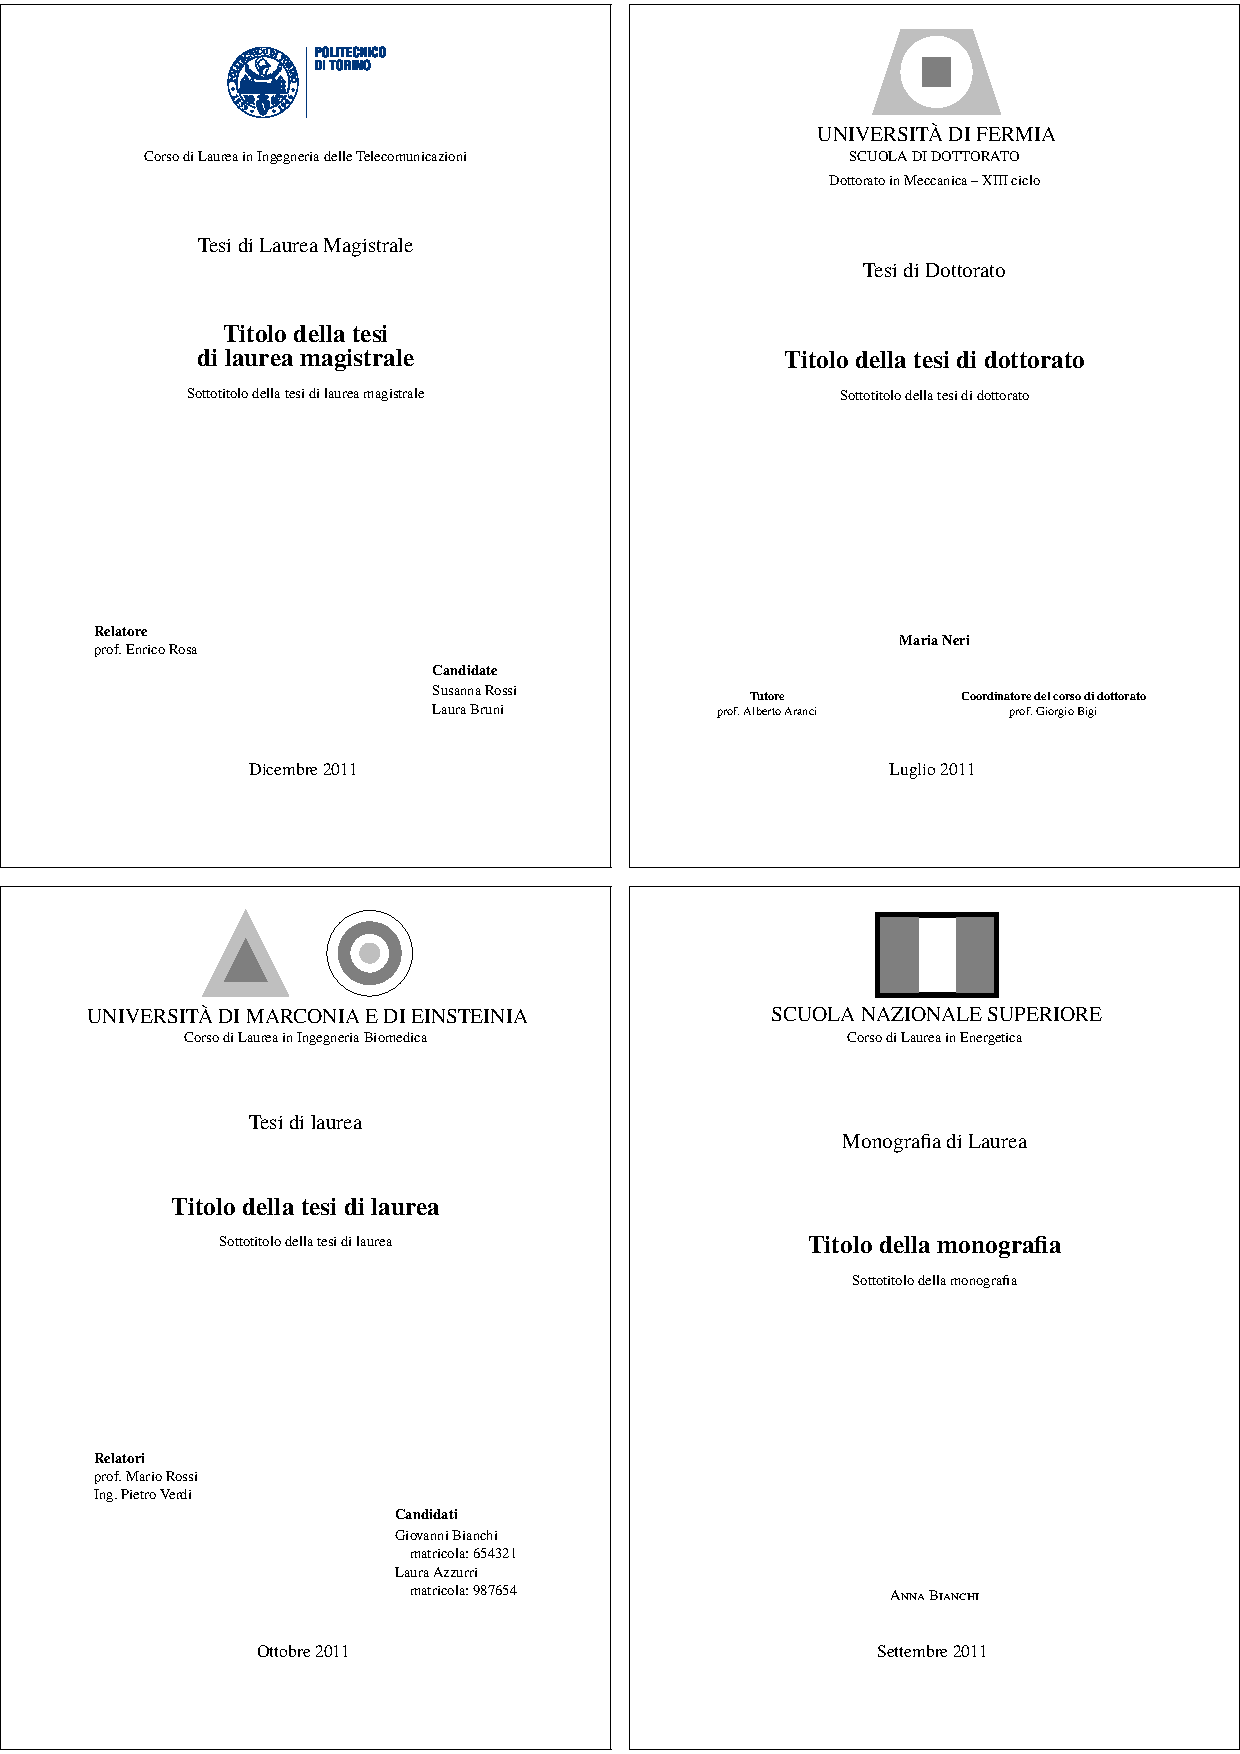
\includegraphics[height=0.875\textheight]{FrontespiziAssemblati1}
\caption[Frontespizi composti con lo stile standard]{Frontespizi composti con lo stile standard. In questo stile mancano i filetti e i loghi delle università possono essere messi in posti diversi della pagina; il nome dell'università può essere presente esplicitamente oppure può essere compreso nel logo.}\label{fig:4frontespizi}
\end{figure}


Nella figura~\ref{fig:altri4frontespizi} sono mostrati invece i quattro frontespizi che si ottengono quando alla classe (o anche al solo modulo \pack{topfront} quando lo si usa con una classe diversa da \class{toptesi}) viene specificata l'opzione \chiave{stile}{classica}. Attenzione: le opzioni \opt{classica}, e quelle che da essa dipendono, come  \opt{oldstyle} e  \opt{autoretitolo}, possono venire specificate al pacchetto senza usare la sintassi \emph{chiave$=$valore} quando questo viene usato con una classe diversa da \class{toptesi}; alcune non hanno molto a che vedere con il frontespizio, sebbene possano venire usate anche all'interno del pacchetto \pack{topfront}. 

In particolare se si volesse comporre il frontespizio con  lo stile \opz{classica} usando la classe \class{book}, ma con il frontespizio composto con \pack{topfront}, basterebbe impostare nel preambolo:
\begin{flushleft}\ttfamily\obeylines
\char92documentclass\oarg{opzioni}\Arg{book}
...
\char92usepackage\Oarg{classica}\Arg{topfront}
...
\char92begin\Arg{document}
\end{flushleft}

Nello stile \chiave{stile}{classica} si nota che il nome dell'ateneo è separato dal resto della pagina da un filetto orizzontale; analogamente l'anno accademico in calce alla pagina è separato da un filetto orizzontale. I candidati sono chiamati ``Laureandi''. Il blocco contenente i nomi dei relatori e correlatori e quello contenente i nomi dei laureandi sono allineati superiormente e non sono sfasati come nello stile standard. La seduta di esame è indicata con la dicitura ``Anno accademico'' in maiuscoletto e l'anno, o l'intervallo di anni è indicato con le cifre arabe minuscole (old style). Con questo stile più classico, il logo o i loghi sono collocati fra i titolo e i blocchi dei relatori e dei laureandi.

Si noti, infine, che in entrambi gli stili esistono esempi con due loghi, per i quali i nomi dei due atenei vanno scritti in forma un poco ellittica, ma piuttosto antiestetica; in generale potrebbero formare una riga così lunga da non entrare nella pagina fisica; più avanti si mostra come comporre i nomi degli atenei in modo che non escano fuori dalla pagina. Si veda  più avanti nel paragrafo~\ref{sec:casi-particolari}.

Lo si potrebbe considerare una ``feature'', una particolarità del pacchetto \TOPtesi.  In realtà non conosco altre classi o moduli di estensione dove sia possibile fare riferimento a diversi loghi e a diversi nomi.

Quello che consiglierei in questi casi sarebbe di aggiungere il nome dell'ateneo al logo, se già non lo contenesse, e lo farei un con un font di contrasto, per esempio con un font senza grazie maiuscolo o maiuscoletto con iniziali maiuscole, magari su due righe collocato sotto il logo vero che non contenga a sua volta già il nome dell'ateneo; come per esempio nel logo modificato mostrato nella figura~\ref{fig:logomodificato}.

\begin{figure}
\centering
\begin{minipage}[t]{30mm}\centering
\includegraphics[width=30mm]{logodue}\\[3pt]
\fontsize{17}{16}\sffamily U\simulatedSC{NIVERSITÀ}\\
\simulatedSC{DI} M\simulatedSC{ARCONIA}
\end{minipage}
\caption{Un logo modificato con l'aggiunta del nome dell'ateneo}\label{fig:logomodificato}
\end{figure}

Fatta questa modifica per tutti i loghi privi del nome dell'università che è necessario usare, si compone il frontespizio con lo stile standard  usando semplicemente un nome vuoto come argomento di \cs{ateneo}. Si veda poco più avanti come usare una pluralità di loghi.


Vale la pena di ricordare che la retrocompatibilità con i comandi \cs{frontespizio} e \cs{frontespizio*} è conservata. 

Perciò merita confrontare le molteplici configurazioni offerte dal modulo \pack{topfront} mediante la tabella comparativa~\ref{tab:modalitaperfrontespizi}.

\begin{table}[!htb]\caption{Varie modalità di composizione del frontespizio}\label{tab:modalitaperfrontespizi}
{\centering
\begin{tabularx}{\textwidth}{*3{>\raggedright X}}\toprule
Comando, ambiente, opzione	& Stile standard	& Stile classica 	\tabularnewline
\midrule
\amb{frontespizio}	& loghi in testa	& loghi in basso	\tabularnewline
\cs{ateneo} vuoto 	& senza nome dell'ateneo	& messaggio d'errore\tabularnewline
\cs{ateneo} non vuoto& Nome dell'ateneo in testa & nome dell'ateneo in testa
\tabularnewline
filetti				& assenti					& presenti			\tabularnewline
\midrule
\amb{frontespizio*}	& loghi in basso			& loghi in basso	\tabularnewline
\cs{ateneo} vuoto	& senza nome dell'ateneo	& messaggio d'errore\tabularnewline
\cs{ateneo} non vuoto& nome dell'ateneo in testa	& nome dell'ateneo in testa	\tabularnewline
filetti				& assenti					& presenti			\tabularnewline
\midrule
\cs{frontespizio}	& come \amb{frontespizio}	&come \amb{frontespizio}
\tabularnewline
\midrule
\cs{frontespizio*}	& come \amb{frontespizio*}	& come \amb{frontespizio*}	\tabularnewline
\midrule
\opz{evenboxes} presente	& relatori e~candidati allineati
					& relatori e~candidati allineati \tabularnewline
\opz{evenboxes} assente	&	relatori e~candidati disallineati
					& relatori e~candidati allineati \tabularnewline 
\bottomrule
\end{tabularx}\par}\vspace{1ex}

\footnotesize
Gli ambienti \amb{ThesisTitlePage} e \amb{FrontespizioTesina} definiti negli altri moduli, si comportano come l'ambiente \amb{frontespizio}; in alcuni di questi moduli l'ambiente accetta anche l'asterisco, con una sintassi particolare, ma con la stessa funzione che svolge nell'ambiente \amb{frontespizio*}.
\end{table}

\goodpagebreak[6]


\begin{figure}[p]\centering

\includegraphics[height=0.875\textheight]{FrontespiziAssemblati2}
\caption[Frontespizi composti con lo stile \texttt{classica}]{Frontespizi composti con lo stile \texttt{classica}. Con questo stile si ha una disposizione diversa delle varie informazioni e i loghi sono sempre posti nella parte inferiore della pagina. Il nome dell'università è sempre presente.}\label{fig:altri4frontespizi}
\end{figure}

\clearpage

\subsection{Comporre il frontespizio della tesi di dottorato della ScuDo}

Con lo stile prodotto dall'opzione \chiave{tipotesi}{scudo} il frontespizio contiene il logo della Scuola (messo a disposizione dei dottorandi dala Segreteria della Scuola; qui viene usata una imitazione per mostrare come appare un logo di forma simile nell'intestazione della dissertazione) e appare come nella figura~\ref{fig:frontescudo} nella pagina~\pageref{fig:frontescudo}. Questo frontespizio è quello prodotto compilando con \LuaLaTeX\ l'esempio costituito dal file \file{toptesi-scudo\discretionary{}{-}{-}example.tex}.

Si noti: il logo della scuola ScuDo contiene il ``marchio'' e il ``logotipo''; il primo è un'immagine; il secondo è la denominazione esatta dell'ente. Pertanto sarebbe assurdo ripetere il nome dell'ente come nome dell'ateneo e nome della struttura nelle solite righe; il modulo \pack{toptesi-scudo.sty} non contiene nemmeno i comandi per impostare questi nomi. Gli altri blocchi di nomi come le loro etichette sono specifici per questo tipo di frontespizio.

Come già detto il retrofrontespizio viene composto con le frasi esposte nella pagina~\pageref{fig:disclaimer}.

\begin{figure}[p]\centering
\frame{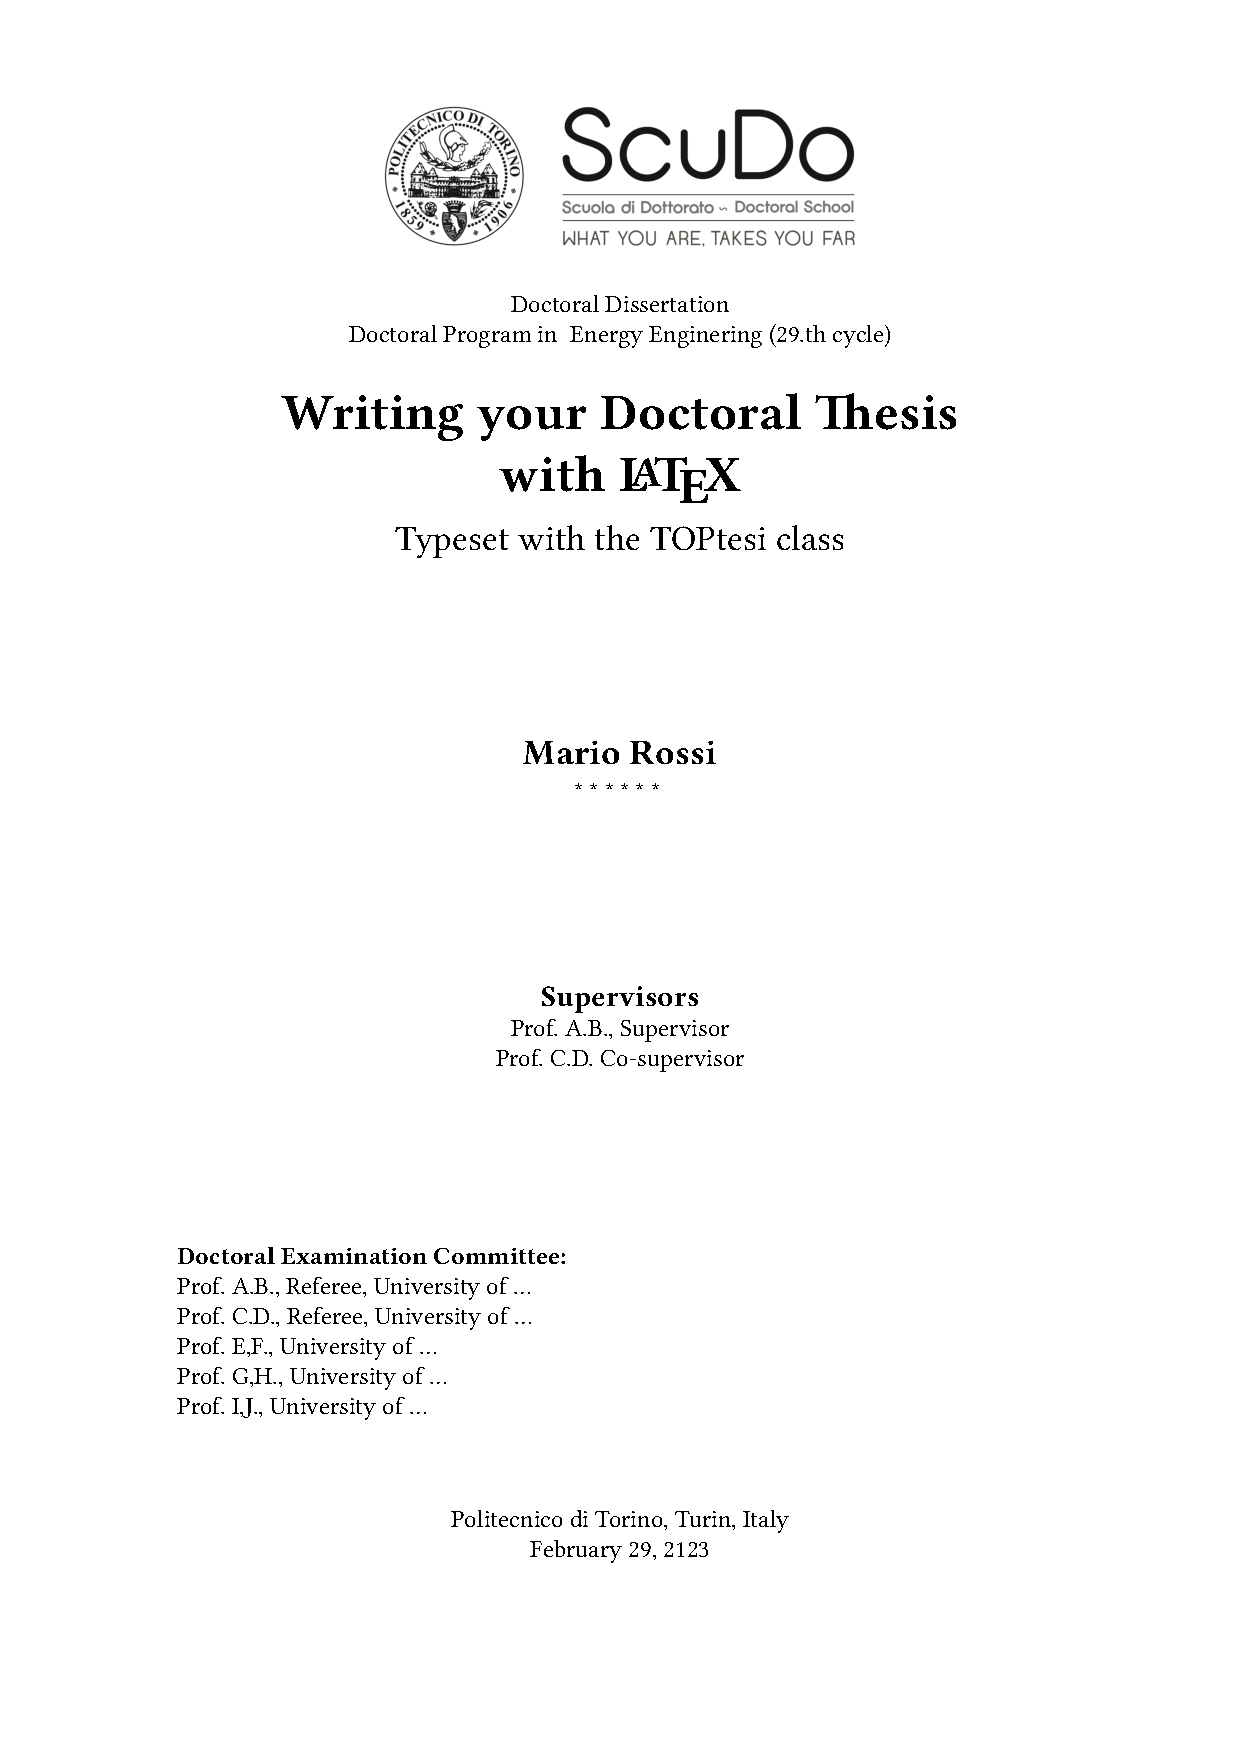
\includegraphics[width=0.9\textwidth]{FrontespizioScudo}}
\caption{Frontespizio della dissertazione della ScuDo}
\label{fig:frontescudo}
\end{figure}

Il codice usato per comporre quel frontespizio è indicato qui di seguito; per i singoli comandi da usare si veda il paragrafo~\ref{sec:scudo}.

\begin{verbatim}
\begin{ThesisTitlePage}
\PhDschoolLogo{Logo-ScuDo}
\ProgramName{Energy Enginering}
\CycleNumber{29.th}
\author{Mario Rossi}
\title{Writing your Doctoral~Thesis\\with \LaTeX}
\subtitle{Typeset with the \TOPtesi class}
\SupervisorNumber{2}
\SupervisorList{%
    Prof.~A.B., Supervisor\\
    Prof.~C.D. Co-supervisor}
\ExaminerList{%
Prof.~A.B., Referee, University of \dots\\
Prof.~C.D., Referee, University of \dots\\
Prof.~E.F., University of \dots\\
Prof.~G.H., University of \dots\\
Prof.~I.J., University of \dots}
\ExaminationDate{February 29, 2123}
\end{ThesisTitlePage}
\end{verbatim}


\subsection{Il frontespizio della tesi triennale}
Per la tesi triennale il frontespizio viene composto specificando alla classe l'opzione \chiave{tipotesi}{triennale} (oppure \chiave{tipotesi}{monografia} -- questa opzione è conservata per retrocompatibilità).

I comandi usabili per impostare le parole fisse e i dati variabili sono sostanzialmente gli stessi indicati per il modulo \pack{topfront}; un cambiamento importante è costituito dal fatto che il titolo della tesi si descrive con lo stesso comando \cs{titolo} usato per le altre tesi, al posto del comando \cs{monografia} (che però è ancora usabile con questo modulo, conservato per retrocompatibilità).

Un altro cambiamento importante è che gli ambienti \amb{frontespizio} e \amb{frontespizio*}, e gli omonimi comandi \cs{frontespizio} e \cs{frontespizio*} non sono più definiti, ma è disponibile solo l'ambiente \amb{ThesisTitlePage} che accetta un asterisco (non delimitato) come primo argomento; la sua sintassi è pertanto la seguente:
\begin{ttsintassi}
\Bambiente{ThesisTitlePage}\meta{*}
\meta{comandi per il frontespizio}
\Eambiente{ThesisTitlePage}
\end{ttsintassi}

La funzione dell'asterisco opzionale è la stessa che si aveva con gli ambienti \amb{frontespizio} e \amb{frontespizio*}, solo che in questo caso l'ambiente è unico e l'asterisco non fa parte del nome: infatti nel comando di chiusura non appare più.

I \meta{comandi per il frontespizio} vengono letti dall'ambiente nel file di configurazione, se esiste, e poi dai comandi esplicitamente indicati per inserire, se occorre, delle stringhe fisse, diverse da quelle preimpostate, e i dati specifici della tesi: autore, titolo, sottotitolo, eccetera. 

I comandi come \cs{ateneo}, \cs{struttura} eccetera agiscono come indicato per il modulo \pack{topfront}.

Le opzioni \chiave{stile}{classica} e \opz{evenboxes} conservano le loro funzioni. 

Un esempio di frontespizio per tesi triennale è dato dal frontespizio di questa stessa documentazione, composto con i comandi:
\begin{verbatim}
\begin{ThesisTitlePage}
\GetFileInfo{toptesi.cls}
\logosede{TITlogoCropped}
\NomeElaborato{Manuale d'uso}
\titolo{Il pacchetto \textsf{TOPtesi}}
\TitoloListaCandidati{}
\sottotitolo{Per comporre tesi al Politecnico di Torino\\
e in molte altre università\\[1ex]
Il pacchetto \textsf{TOPtesi} contiene la classe omonima 
e diversi altri file per comporre tesi di diverso tipo\\[1ex]
Questa documentazione fornisce anche le linee guida per comporre 
una tesi rispettando certe regole tipografiche}
\sedutadilaurea{Pacchetto \textsf{toptesi} versione 
\fileversion\ del \filedate}
\retrofrontespizio{Questo testo è libero secondo 
le condizioni stabilite dalla \LaTeX Project Public 
Licence (LPPL) riportata nell'appendice~\ref{ch:LPPL} 
alla pagina~\pageref{ch:LPPL}.
 
\bigskip
 
\noindent Composto con \ifPDFTeX \pdfLaTeX\else 
\ifXeTeX\XeLaTeX\else\ifLuaTeX\LuaLaTeX\else 
un programma sconosciuto\fi\fi\fi\ il \today
\vspace*{5\baselineskip}}
\end{ThesisTitlePage}
\end{verbatim}

Naturalmente in una vera tesi triennale la composizione del frontespizio e dell'eventuale retrofrontespizio è in generale molto più semplice; ma anche nel frontespizio di questo documento sono bastati poco meno di una dozzina di comandi per definire tutto il frontespizio e il retro del frontespizio.
 
\subsection{Il frontespizio della tesi magistrale}
Per la tesi magistrale il frontespizio viene composto specificando alla classe l'opzione \chiave{tipotesi}{magistrale}.

I comandi usabili sono sostanzialmente gli stessi che fornisce il modulo \pack{topfront}, con alcune differenze. Innanzi tutto, e in modo del tutto ovvio, non sono disponibili i comandi di \pack{topfront} che si riferiscono specificatamente agli altri tipi di tesi triennale e dottorale. Poi è disponibile l'ambiente \amb{ThesisTitlePage} con le stesse caratteristiche descritte per l'omonimo ambiente per il modulo relativo alla tesi triennale. Si richiama l'attenzione sull'uso dell'asterisco da usare facoltativamente come primo token dopo l'apertura dell'ambiente.

In realtà per retro compatibilità gli ambienti \amb{frontespizio} con o senza asterisco e i comandi \cs{frontespizio} con o senza asterisco, sarebbero ancora disponibili, ma se ne scoraggia l'uso, raccomandando la preferenza per il nuovo ambiente \amb{ThesisTitlePage}.

Nulla cambia in merito all'opzione  \chiave{stile}{classica} e all'opzione specificata con \opz{evenboxes} e ai diversi aspetti che queste opzioni, unite all'asterisco facoltativo, producono sul frontespizio della tesi magistrale.


\subsection{Il frontespizio della tesi dottorale}
La tesi dottorale di cui si parla in questa sezione non riguarda la tesi della scuola di dottorato del Politecnico di Torino, per la quale esiste l'apposita opzione e l'apposito modulo. Qui si parla di tesi dottorali da comporre secondo regole di altri atenei, se queste sono compatibili con gli stili disponibili in \TOPtesi; qualora non lo fossero, bisogna ricorrere a un frontespizio completamente personalizzato mediante l'opzione \chiave{tipotesi}{custom}.

In ogni caso il modulo per la composizione delle tesi dottorali ``generiche'' si invoca specificando l'opzione \chiave{tipotesi}{dottorale}. Questo modulo non differisce granché dal modulo generico \pack{topfront}, salvo il fatto che manca di tutti i comandi che si riferiscono specificatamente alle tesi triennali e magistrali.

Anche per questo tipo di tesi è disponibile l'ambiente \amb{ThesisTitlePage} per comporre il frontespizio; come negli altri casi accetta un asterisco facoltativo come primo token dopo l'apertura dell'ambiente. A differenza del modulo per le tesi magistrali non conserva gli ambienti \amb{frontespizio} con o senza asterisco e i comandi \cs{frontespizio} con o senza asterisco.

Nuovamente le opzioni \chiave{stile}{classica} e \opz{evenboxes} unite all'asterisco facoltativo dell'ambiente \amb{ThesisTitlePage}, producono gli stessi effetti già descritti per gli altri moduli.

\subsection{Il frontespizio della tesina}
Per la tesina da presentare all'esame di stato per il conseguimento del diploma di maturità il frontespizio  è evidentemente diverso da quello delle tesi universitarie. Un esempio è mostrato nella figura~\ref{fig:frontepizio-tesina}.

\begin{figure}[p]
\fbox{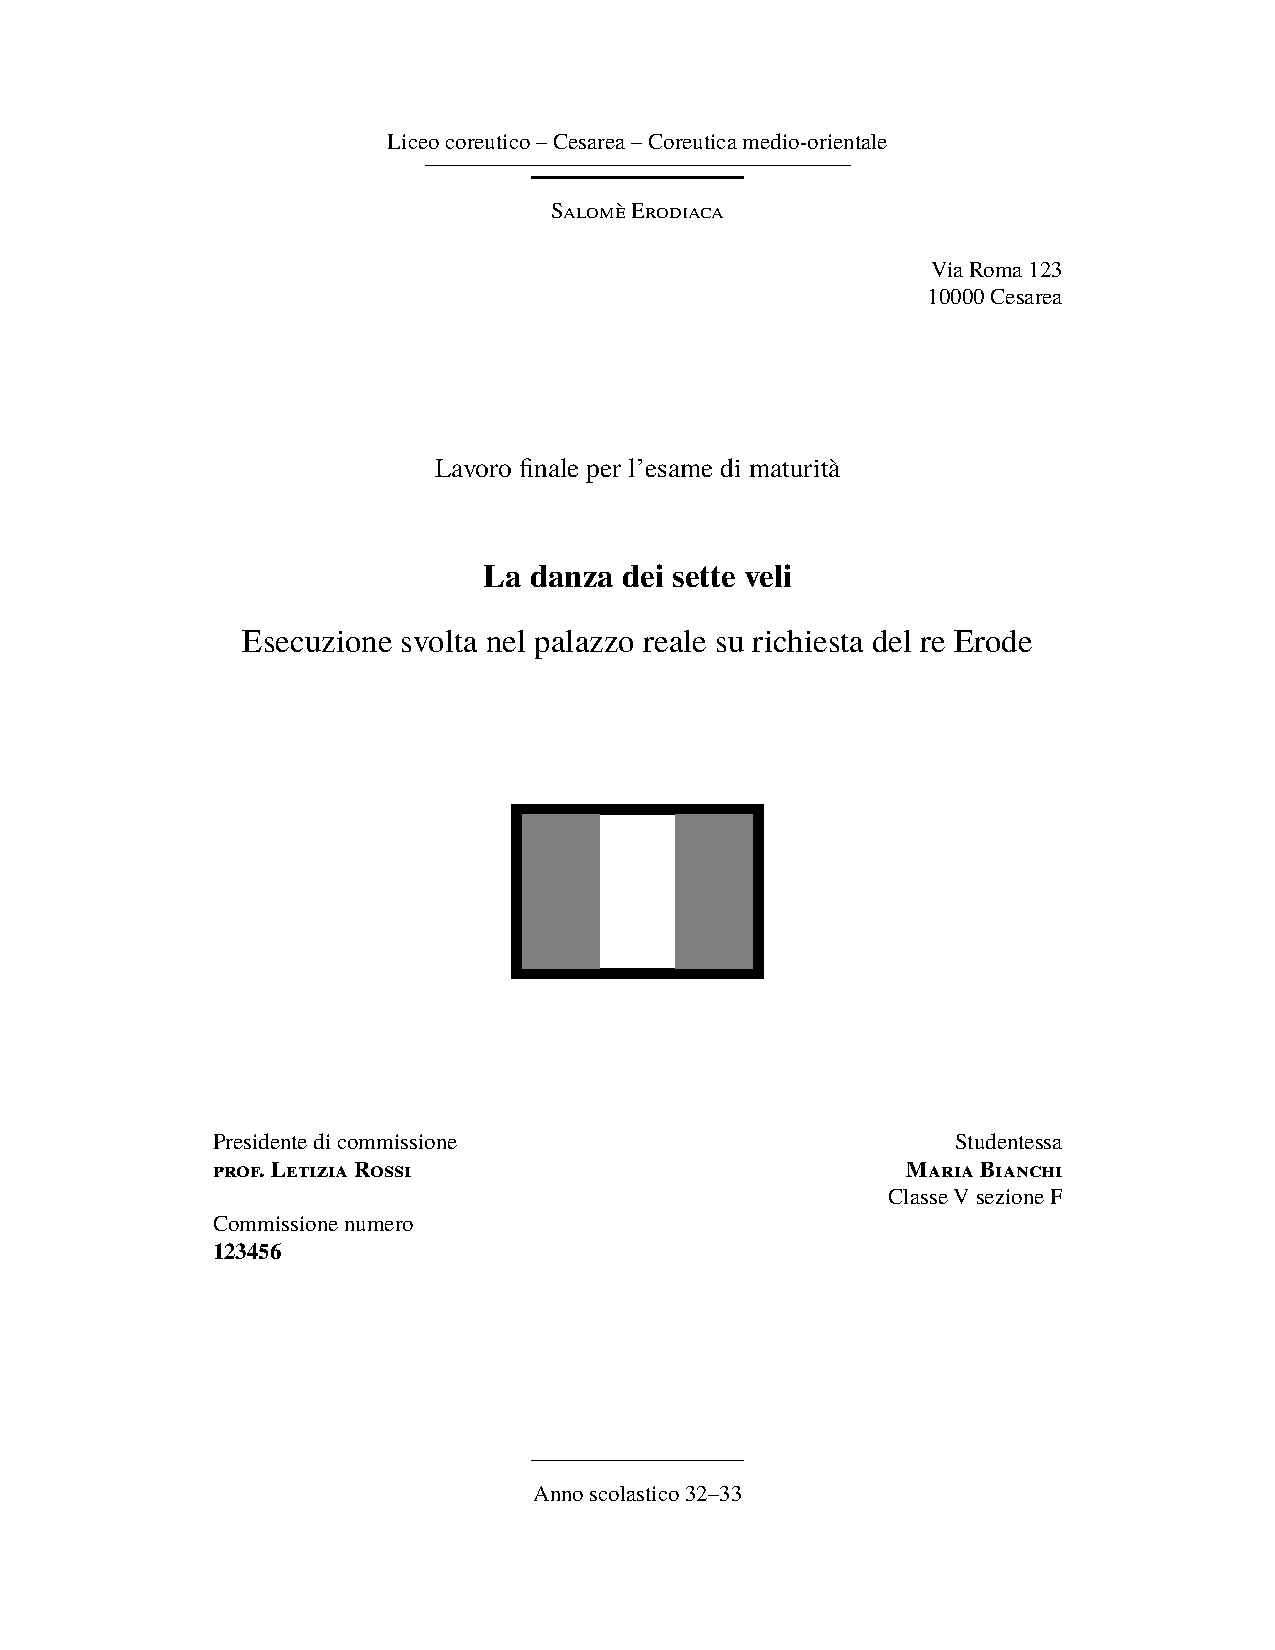
\includegraphics[width=\dimexpr\textwidth-2\fboxrule-2\fboxsep]{Frontespizio-sss}}
\caption{Esempio di frontspizio per una tesina}
\label{fig:frontepizio-tesina}
\end{figure}

Per comporre la tesina bisogna specificare la chiave \chiave{tipotesi}{sss}; questa chiave implica il caricamento di alcuni pacchetti aggiuntivi e la necessità di usare dei comandi specifici per immettere i dati necessari.

Senza specificare altro \TOPtesi usa i font CM-Super; sarebbe meglio richiedere nel preambolo i font Latin Modern mediante il pacchetto \pack{lmodern}; meglio ancora con il pacchetto \pack{cfr-lm} che dispone di molte opzioni e usa meglio le potenzialità dei font Latin Modern. Abituati come sono ad usare i comuni word processor, i maturandi preferiscono usare i font Times; in questo caso raccomanderei di usare i Times extended, mediante il pacchetti \pack{newtxtext} e \pack{newtxmath}, rispettivamente per i font testuali e per quelli matematici; invece, preferendo un font più facilmente leggibile e un pochino più largo, suggerirei i font Palatino extended da richiamare con i pacchetti \pack{newpxtext} e \pack{newpxmath}.

Va notato subito che è possibile inserire il logo della scuola, ma ovviamente bisogna richiederlo alla scuola, la quale potrebbe negarlo; non è cattiveria; semplicemente il logo è un suo simbolo legale e potrebbe venirne fatto un uso improprio; la scuola potrebbe però disporre di un logo secondario per questi scopi. Nella figura~\ref{fig:frontepizio-tesina} è stato usato un disegno di fantasia, solo per mostrare dove verrebbe inserito; se non si inserisce nulla, lo spazio inutilizzato viene automaticamente ridistribuito fra gli altri spazi.

Vediamo subito i pacchetti aggiuntivi che bisogna \emph{evitare di ricaricare}.
\begin{description}[noitemsep]
\def\Item[#1]{\normalfont\item[\pack{#1}]}
\Item[amsmath] e \pack{amsthm} 
   sono caricati indipendentemente dal programma di composizione 
   usato per comporre la tesina; servono per comporre matematica 
   un po' complessa e per definire altri tipi di enunciati da 
   mettere in evidenza; bisogna leggerne la documentazione per 
   usarli in modo appropriato.
\Item[amssymb]
   viene caricato solo se si usa come programma di composizione 
   \pdfLaTeX; serve per avere accesso ad un altro paio di 
   centinaia di simboli matematici adatti a complementare la 
   matematica componibile con il precedente pacchetto \pack{amsmath}.
\Item[unicode-math] 
   viene caricato quando \LuaLaTeX\ o \XeLaTeX\ vengono usati 
   come programmi di composizione. L'utente però deve specificare 
   nel preambolo quale font OpenType matematico vuole usare.
\Item[xparse] e \pack{xspace} e \pack{xcolor} 
   sono funzionali per la classe, ma le loro funzionalità possono 
   essere usate anche dall'utente. Ovviamente è necessario leggere 
   la documentazioni di quei pacchetti per usarli correttamente.
\Item[calc] e \pack{ifthen}
   sono caricati per mettere l'utente nelle condizioni di eseguire
   semplici calcoli aritmetici e/o logici se per caso desidera 
   crearsi delle macro personali. Non è necessario farne uso perché
   da molti anni i programmi di composizione del sistema \TeX 
   sanno fare queste operazioni senza l'uso di pacchetti esterni; 
   tuttavia diversi utenti preferiscono usare questi pacchetti.
\Item[multirow]
   viene caricato a beneficio di coloro che vogliono imitare 
   le tabelle composte con i soliti word processor che sono 
   in grado di comporre celle che si svolgono su più righe; 
   tipograficamente parlando non è una pratica molto rigorosa, 
   ma in rare circostanze poterebbe essere utile.
\Item[booktabs]
   invece serve per comporre tabelle professionali senza filetti 
   verticali e senza  quei filetti orizzontali che vengono 
   solitamente usati dai word processor.
\end{description}
Non si sono caricati pacchetti particolari per la composizione della bibliografia; lo studente ha tre possibilità:
\begin{enumerate}[noitemsep]
\item Compone la bibliografia a mano servendosi dell'ambiente 
   \amb{thebibliography}; non è complicato se la bibliografia 
   è breve; diventa molto complicato con una lunga bibliografia 
   a causa della moltitudine di errori che sfuggono ma, 
   specialmente, per la disuniformità della composizione delle 
   singole voci.
\item Si usa il pacchetto \pack{natbib} e si crea un database 
    bibliografico con il programma \prog{jabref} o con 
    \prog{bibdesk} (quest'ultimo, solo per il Mac, è già 
    installato solo per il fatto di avere installato il sistema 
    \TeX usando Mac\TeX). Predisposto il database bibliografico, 
    si usa l'elaboratore \prog{bibtex} per estrarre e formattare 
    alla \LaTeX gli estremi delle opere da citare, e poi il 
    comando \cs{printbibliography} e i vari tipi di comandi 
    \cs{cite} predisposti da \pack{natbib} permettono sia di 
    comporre la bibliografia nel documento, sia di citare 
    correttamente le opere elencate. Conviene leggere la 
    documentazione relativa ai databse bibliografici dando 
    da terminale il comando \texttt{texdoc bibtex}, in particolare 
    il suo paragrafo~3.
\item Si usa il database bibliografico come nel caso precedente, 
   ma si usa il pacchetto \pack{biblatex} e l'elaboratore di 
   database \prog{biber} per ottenere un risultato impeccabile; 
   la documentazione di \pack{biblatex} va letta con attenzione, 
   perché questo è un pacchetto molto performante e richiede di 
   essere usato con assoluta precisione.
\end{enumerate}

Invece i comandi da usare per comporre il frontespizio sono raccolti nelle tabelle del capitolo~\ref{cap:comandispecifici}.
Qui si ripetono con una descrizione a parole, non nella forma stringata delle tabelle. Si ricorda che, come per gli altri tipi di tesi; si può disporre di un file di configurazione e che i comandi per il frontespizio vanno inseriti all'interno del ambiente \amb{FrontespizioTesina}; questo legge, se c'è, il file di configurazione, poi esamina i comandi che l'utente ha inserito fra lo statement di apertura e quello di chiusura. Se l'utente ha ripetuto qualche comando già presente nel file di configurazione, il comando dell'utente ha la prevalenza.

\begin{description}[noitemsep]
\def\Item[#1]{\normalfont\item[\cs{#1}]}
\Item[SSSlogo]
   Serve per definire il nome, senza estensione, del file che 
   contiene l'immagine del logo della scuola;  se questo comando 
   non viene dato, non viene inserito nulla nel frontespizio. 
   Il file può avere solo certi formati di immagine corrispondenti 
   alle estensioni \file{.pdf}, \file{.eps}, \file{.png}, e 
   \file{.ipg}; i primi due formati possono essere vettoriali 
   e, se lo sono davvero\footnote{Potrebbero contenere al loro 
   interno una matrice di punti colorati, come i formati del 
   secondo tipo, quindi non sarebbero dei veri formati 
   vettoriali.}, sono riproducibili con qualunque fattore di 
   scala; i secondi due formati sono a matrici di punti e la 
   loro resa può essere scadente se la densità di pixel al 
   pollice è inferiore ai 150\unit{pxl/inch}. I primi formati 
   sono certamente preferibili. La sintassi è:
\begin{ttsintassi}
\cs{SSSlogo}\marg{nome del file}
\end{ttsintassi}
%
\Item[NomeTesina] 
   serve per impostare il nome dell'elaborato; la stringa di 
   default è ``Tesina di maturità'', ma l'utente può cambiarla 
   a suo piacimento; potrebbe persino indicare una stringa vuota. 
   La sintassi è:
\begin{sintassi}
\cs{NomeTesina}\marg{nome dell'elaborato}
\end{sintassi}
\Item[NomeCandidato]
   Imposta l'indicazione da scrivere sopra il nome dello studente;
   l'impostazione di default scrive ``Studente'' oppure 
   ``Studentessa'' a seconda che il nome del maturando venga 
   introdotto mediante il comando \cs{studente} o 
   \cs{studentessa}; l'utente che usa questo comando 
   \cs{NomeCandidato} evidentemente vuole cambiare 
   l'indicazione preimpostata, quindi non ha bisogno di 
   scrivere comandi complessi per distinguere il maschile 
   dal femminile; il maturando sa sicuramente di che genere 
   è, quindi mette un nome del genere corrispondente. 
   La sintassi è:
   \begin{sintassi}
   \cs{NomeCandidato}\marg{Etichetta del maturando}
   \end{sintassi}
\Item[IndirizzoMiur] imposta l'indirizzo speciale della scuola
   come risulta al Ministero. Questa indicazione è facoltativa. 
   Se si vuole impostare questo indirizzo, la sintassi è:
 \begin{sintassi}
 \cs{IndirizzoMiur}{Indirizzo speciale del Ministero}
 \end{sintassi}
\Item[OpzioneMiur]
   indicazione facoltativa che specifica la destinazione culturale 
   come risulta al Ministero; se la si vuole indicare, la sintassi è:
   \begin{sintassi}
   \cs{OpzioneMiur}\marg{opzione ministeriale}
   \end{sintassi}
\Item[TipoScuola]
   imposta la denominazione generica della scuola, per esempio 
   ``Liceo Classico'', oppure ``Istituto Tecnico Industriale 
   di Stato'' o quant'altro si riferisca alla scuola specifica 
   del maturando. Nessun valore preimpostato. Lo si imposta 
   con la sintassi:
   \begin{sintassi}
   \cs{TipoScuola}\marg{denominazione generica della scuola}
   \end{sintassi}
\Item[NomeScuola]
   imposta il nome della persona o dell'evento a cui è intitolata 
   la scuola, per esempio ``Vittorio Alfieri'', ``Sandro Pertini'', 
   e simili. Non tutte le scuole sono intitolate a qualcuno o a 
   qualche evento importante; se si vuole impostare questo nome, 
   la sintassi è:
   \begin{sintassi}
   \cs{NomeScuola}\marg{intitolazione}
   \end{sintassi}
\Item[SedeScuola] 
   imposta la sede della scuola; può consistere del solo nome 
   della città dove ha sede la scuola, oppure può essere 
   l'intero indirizzo civico; il comando accetta anche 
   argomenti che contengono segni di ``a~capo'' (\cs{\char92}); 
   la sintassi è:
   \begin{sintassi}
   \cs{SedeScuola}\marg{sede della scuola}
   \end{sintassi}
\Item[AnnoScolastico]
   imposta l'anno scolastico durante il quale viene svolto 
   l'esame di stato; può essere una indicazione abbreviata, 
   del tipo ``33--34'', oppure completa ``2033--2034''. 
   Lo si imposta con la sintassi:
   \begin{sintassi}
   \cs{AnnoScolastico}\marg{anno scolastico}
   \end{sintassi}
\Item[titolo]
   imposta il titolo della tesina. È opportuno mantenere il 
   titolo molto lapidario affinché possibilmente occupi solo 
   una riga, al massimo due righe; nell'indicare dove andare 
   a capo si metta il segno \verb|\\| prima di un articolo, 
   di una preposizione, di un breve avverbio, in modo da non 
   andare a capo dopo simili parole. Se si devono aggiungere 
   dettagli al titolo, lo si faccia usando il successivo 
   comando \cs{sottotitolo}. La sintassi è:
   \begin{sintassi}
   \cs{titolo}\marg{titolo della tesina}
   \end{sintassi}
\Item[sottotitolo]
   imposta facoltativamente il sottotitolo; questo può essere 
   composto anche da più enunciati, come fatto nel frontespizio 
   di questa documentazione. Lo si può impostare con la sintassi:
   \begin{sintassi}
   \cs{sottotitolo}{un sottotitolo di uno o più enunciati}
   \end{sintassi}
   Di nuovo si raccomanda di andare a capo solo prima 
   di articoli, preposizioni, congiunzioni e simili brevi 
   parole usando esplicitamente il comando\verb|\\|.
\Item[studente]
   o \textbf{\cs{studentessa}} imposta il nome e cognome del 
   maturando; si raccomanda di mettere sempre il cognome dopo 
   il nome; la sintassi valida per entrambi i comandi è la 
   seguente:
   \begin{sintassi}
   \cs{studente}\marg{Nome Cognome}\oarg{sigla della classe}
   \end{sintassi}
   La \meta{sigla della classe} è facoltativa; se è costituita
   da una stringa non nulla, questa viene scritta di default 
   sotto il nome del maturando, rientrata e in carattere 
   normale; se si vuole una indicazione diversa, per esempio 
   in linea con il nome del maturando, si deve ridefinire la 
   macro \cs{IDlabel}; questa è predefinita così:\\[1ex]
 \texttt{\string\newcommand*\string\IDlabel[1]\{\string\\%
 \string\quad\{\string\normalfont\string\normalsize\#1\}\char92\textvisiblespace \}}\\[1ex]
   Attenzione: il nome del maturando viene composto in 
   maiuscoletto nero; se il font in uso non ne dispone, esso 
   viene composto in tondo nero. 
   Per la \meta{sigla della classe} 
   si possono usare indicazioni lapidarie come ``{V F}'', o 
   espressioni più dettagliate come, ad esempio, ``{V sezione F}'' o 
   ``{V indirizzo linguistico}''.
\Item[Presidente]
   imposta il nome del presidente della commissione d'esame; 
   va preceduto dal suo appellativo professionale, in genere solo 
   \verb*|prof.\ |; evitare ``prof.ssa'' la cui versione 
   abbreviata in modo burocratico non serve, visto che 
   l'appellativo è seguito dal nome proprio della persona. 
   Ovviamente il nome va sempre prima del cognome. La sintassi è:
   \begin{sintassi}
   \cs{Presidente}\marg{appellativo Nome Cognome}
   \end{sintassi}
   Attenzione: il nome di questa persona, compreso l'appellativo, 
   viene composto in maiuscoletto nero; se il font in uso non ne 
   dispone, esso viene composto in tondo nero; usando il 
   maiuscoletto, l'appellativo va indicato usando solo lettere 
   minuscole.
\Item[NumeroCommissione]
   imposta una informazione non obbligatoria, costituito dal 
   numero identificativo assegnato dal Ministero alla specifica 
   commissione d'esame. Lo si imposta con la sintassi:
   \begin{sintassi}
   \cs{NumeroCommissione}\marg{numero identificativo della 
   \qquad commissione}
   \end{sintassi}
\end{description}

Come esempio di applicazione si veda il file del pacchetto \TOPtesi,  denominato \file{toptesi\discretionary{}{-}{-}example\discretionary{}{-}{-}sss.pdf}.

\subsection{Il frontespizio ``custom''}
Come già spiegato, l'opzione \chiave{tipotesi}{custom} impedisce il caricamento degli altri moduli di \TOPtesi,  ma consente all'utente di caricarsi un suo file personale per la composizione del frontespizio; alternativamente l'utente può crearsi un frontespizio completamente personalizzato usando l'ambiente \amb{titlepage}.

Per seguire questa strada, qui posso dare solo delle indicazioni generiche.
\begin{enumerate}[noitemsep]
\item Aperto l'ambiente \env{titlepage} sarebbe opportuno cambiare localmente la geometria del layout della pagina, specificandolo con
\begin{flushleft}
\cs{thispagestyle}\marg{stile}
\end{flushleft}
dove \meta{stile} è stato precedentemente definito usando il pacchetto \pack{geometry} o altri pacchetti. Sarebbe opportuno ridefinire i due margini interno ed esterno in modo che siano uguali. Qualcuno desidera apportare  un piccolo spostamento verso l'esterno di non più di 5\,mm per compensare la curvatura della prima pagina; questa curvatura dipenderebbe dal modo di confezionare/legare la tesi; di solito  con una  brossura ben eseguita o una legatura a filo, non è necessario apportare questa correzione; con una tesi spillata con punti metallici, probabilmente una piccola correzione non guasterebbe; però questa correzione è concepita per le pagine interne ma, siccome il frontespizio è la prima pagina della tesi, la curvatura della pagina è irrilevante e questo piccolo spostamento è del tutto superfluo.
%
\item Non è necessario che i margini laterali  siano complessivamente equivalenti ai margini del corpo della tesi, ma non guasta se lo sono.
%
\item Per la disposizione verticale del testo, sarebbe preferibile che i margini superiore e inferiore siano otticamente equivalenti; questo dipende dal fatto che il primo elemento in alto sia, per esempio, il nome dell'ateneo scritto con caratteri relativamente alti e neri, oppure sia il logo dell'università, che può essere alto, ma di solito non è tanto largo. Inoltre lo stile della pagina non deve presentare né testatina con il suo spazio di separazione del testo, né piedino, con il suo spazio di separazione dal testo, e non deve contenere il numero della pagina.
%
\item Il laureando deve provvedere autonomamente alle spaziature verticali fra un elemento e l'altro; deve decidere se certe parti siano da comporre in modo centrato, oppure in bandiera col palo a sinistra o a destra, se certe parti debbano essere affiancate e come debbano essere distanziate. 
%
\item Il laureando deve naturalmente scegliere collezione, codifica, famiglia, serie, forma, corpo e scartamento dei font che usa per le varie parti del testo. Una possibile scelta per un font senza grazie da usare per il nome dell'ateneo, potrebbe essere quella di riferirsi alla collezione Iwona, scegliendo la famiglia \Font{Iwona} con codifica \opt{T1} nella serie \texttt{m} con la forma \texttt{n}, nel corpo di \texttt{15}\,pt, e con lo scartamento poco interlineato di soli \texttt{17}\,pt. Dovrebbe quindi chiamare il pacchetto \pack{iwona} nel preambolo e per usare il font dovrebbe usare la serie di comandi
\begin{flushleft}\ttfamily
\cs{fontsize}\Marg{15}\Marg{17}\cs{usefont}\Marg{T1}\Marg{iwona}\Marg{m}\Marg{n} 
\end{flushleft}
quando compone quell'informazione; dovrebbe curare di fare questa operazione dentro un gruppo al fine di mantenere queste impostazioni solo per la scrittura di quella informazione. Sarebbe meglio definirsi un comando personale per evitare di dover ogni volta introdurre quella serie di istruzioni, con il rischio di commettere anche il più piccolo errore di battitura e quindi di generare fastidiosi messaggi d'errore.
\end{enumerate}

Non scendo in ulteriori dettagli; l'utente che volesse comporre un frontespizio molto personalizzato per questa via, deve sapere quello che sta facendo e deve farlo con la dovuta competenza tipografica e del linguaggio \LaTeX. I risultati estetici dipendono fortemente da queste sue capacità.

Un esempio di un frontespizio costruito per questa via è quello  utente creato con la pagina in \opt{landscape}; era destinato ad una tesi veramente originale nel formato ``panoramico'' dovuta al fatto che conteneva molti disegni. Per venire incontro alle queste esigenze è stato scritto questo codice dove i dati sensibili sono sostituiti con nomi di fantasia:\label{proc:titlepage}
\begin{verbatim}
\documentclass [titlepage]{article}
\usepackage[a4paper,left=3cm,bottom=1.5cm,right=3cm,top=1.5cm,%
             landscape]{geometry}
\usepackage{graphicx}
\usepackage[T1]{fontenc}
\usepackage{iwona}
\usepackage[italian]{babel}
\usepackage[utf8]{inputenc}   
\nofiles 

\newcommand {\institutionfont}{\fontsize {22}{30}\scshape}
\newcommand {\divisionfont}{\fontsize {16}{20}\rmfamily}
\newcommand {\pretitlefont}{\fontsize {16}{16}\rmfamily}
\newcommand {\titlefont}{\fontsize {18}{22}\usefont{T1}%
                {iwona}{bx}{n}}
\newcommand {\fixednamesfont}{\fontsize {14}{17}\mdseries}
\newcommand {\namesfont}{\fontsize {15}{18}\bfseries}
\newcommand {\footfont}{\fontsize {15}{18}\rmfamily}

\begin{document}

\begin{titlepage}
%
  \centering
    
    \begin{minipage}[c]{.475\textwidth}\centering
    \includegraphics[width=30mm]{logouno}\\[\baselineskip]
    {\institutionfont UNIVERSITÀ DI PAPEROPOLI\par}
    \end{minipage}
    \hfill
    \begin{minipage}[c]{0.475\textwidth}\centering
    {\divisionfont FACOLTÀ DI PENNUTOLOGIA\\[1ex]
     Corso di~laurea in~ingegneria del~volo~battente\par}
    \end{minipage}\vspace{\stretch{1}}
%    
    {\pretitlefont Tesi di laurea\par}\vspace{\baselineskip}
    {\titlefont STUDIO ANALITICO DELLE PROPRIETÀ DELLE PENNE,
    INCLUSE QUELLE DEGLI UCCELLI ACQUATICI, IN PARTICOLARE QUELLE
    DEI~CIGNI NERI AUSTRALIANI\par}
    \vspace{\stretch{0.7}}
    
    \makebox[\textwidth]{\null\hfill\def\arraystretch{1.5}%
    \begin{minipage}[t]{.375\textwidth}\raggedright  
    \begin{tabular}[t]{@{}l@{}}
    \fixednamesfont Relatore\\
    \namesfont Prof. ing. Mario Rossi\\[1ex]
    \fixednamesfont Correlatore\\
    \namesfont Dott. ing. Giuseppe Scapigliati
    \end{tabular}
    \end{minipage}
    \hfill
    \begin{minipage}[t]{.375\textwidth}\raggedleft
    \begin{tabular}[t]{@{}l@{}}
    \fixednamesfont Candidato\\
    \namesfont Alfredo Bianchi
    \end{tabular}
    \end{minipage}\hfill\null}
%    
    \vspace{\stretch{1}}
%    
    {\footfont Anno accademico 2111--2112\par}
%    
\end{titlepage}
\end{document}
\end{verbatim}

Nel codice precedente appaiono alcuni comandi per i font i cui nomi per le corrispondenti dichiarazioni sono ispirati a quelli contenuti nel pacchetto \pack{frontespizio}, ma i nomi sono irrilevanti, nel senso che qualunque altro nome sarebbe stato altrettanto valido; però è utile che i nomi dei dei comandi relativi ai font siano scelti in modo che ricordino la funzione per la quale sono stati definiti.

La pagina che l'utente ha ottenuto è contenuta nella figura~\ref{fig:frontespizio-landscape}. Per inserirla come frontespizio della tesi egli ha poi usato il pacchetto \pack{pdfpages} che permette di inserire pagine scelte di un file PDF in un documento da comporre con uno qualsiasi dei tre programmi di composizione. Se ne veda la documentazione aprendo un terminale o un prompt dei comandi, scrivendoci dentro \verb|texdoc pdfpages| e poi premendo il tasto \tasto{invio}.

\begin{figure}[t]\frame{
\includegraphics[width=\textwidth]{FrontespizioLandscape}}
\caption{Frontespizio con l'orientamento \opt{landscape} ottenuto con l'ambiente \env{titlepage}}\label{fig:frontespizio-landscape}
\end{figure}

Volendo, si potrebbe mettere tutto il codice precedente in un file personale, per esempio \file*{IlMioFrontespizio.tex}, e immetterlo nel corpo della tesi semplicemente usando il comando \cs{input}. Il corpo della tesi risulta alleggerito e la sua gestione e manutenzione ne risulta semplificata.



\subsection{Il frontespizio composto con \texorpdfstring{\pack*}{}{frontespizio}}\label{sec:solofrontespizio}

Potrebbe essere necessario comporre il frontespizio in modo diverso da come viene composto tramite i comandi contenuti nei vari moduli di \TOPtesi. 


Ci sono diversi motivi per i quali un laureando o dottorando vorrebbe comporre un frontespizio diverso da quelli predefiniti dai moduli di  \TOPtesi. 
\begin{enumerate}[noitemsep]
\item Le specifiche per le tesi di una data università sono inconciliabili con quelle impostate da tutti i moduli di \TOPtesi. 
\item Le informazioni da inserire nel frontespizio sono diverse da quelle impostate dai moduli di \TOPtesi. 
\item Il laureando non deve soddisfare a specifiche particolari ma vuole comporre un frontespizio personalizzato a suo piacimento.
\end{enumerate}

A seconda dei motivi per i quali il laureando non vuole o non può usare il layout e la strutturazione del frontespizio predisposto da \TOPtesi,  il laureando deve ricorrere a \chiave{tipotesi}{custom}, di cui si è già parlato, oppure a \chiave{tipotesi}{frontespizio}, la quale provvede a richiamare il pacchetto esterno \pack{frontespizio} rinunciando alle funzionalità di \TOPtesi. 

Questa seconda via può dare risultati buoni, grazie alla possibilità di personalizzazione che offre il pacchetto \pack{frontespizio}. Ma non si può fare sempre tutto; anche questo pacchetto è preimpostato per produrre  il frontespizio  nel formato di carta A4 e con due stili, ``standard'' ed  ``elements'' specifico per l'uso con la classe \class{suftesi}. Più avanti indicherò come produrre frontespizi con altri formati di carta.

Esistono altri pacchetti, oltre a \pack{frontespizio}, per comporre pagine di titoli; ma per le tesi questo pacchetto sembra il più indicato. Definisce comandi per inserire virtualmente qualsiasi informazione necessaria per un frontespizio di tesi di laurea triennale, magistrale o dottorale; per impostazione predefinita tutte le informazioni fisse sono in italiano, ma ciascuna può essere modificata come si vuole in qualsiasi lingua.

Per seguire questa strada bisogna specificare l'opzione \chiave{tipotesi}{frontespizio} alla classe. Questa opzione imposta tutte le variabili booleane necessarie per evitare dimenticanze e possibili errori, impedisce il caricamento di ogni altro modulo relativo  ai vari tipi di tesi, e richiama il pacchetto esterno \pack{frontespizio} di cui è necessario conoscere i dettagli dalla sua documentazione.

Questo pacchetto \pack{frontespizio} produce un file ausiliario \meta{nome del main file della tesi}\file{-frn.tex} per comporre il frontespizio vero e proprio; questo implica che per disporne come frontespizio del documento finito, bisogna comporre anche questo file ausiliario.

Precisamente tutte le informazioni riguardanti il frontespizio devono essere messe dentro un ambiente \amb{frontespizio} collocato dopo l'istruzione \Bambiente{document}. Qui si metteranno i comandi per definire il nome del o dei candidati, il nome del o dei relatori e degli eventuali correlatori, il nome dell'università, il nome del corso di laurea, il nome del tipo di tesi, il titolo e il sottotitolo della tesi, eccetera.

Eseguendo \prog{pdflatex} oppure \prog{xelatex} o \prog{lualatex} viene prodotto il file ausiliario; se la tesi ha il main file che si chiama \texttt{MarioRossiTesiMagistrale.tex}, dopo averlo compilato, nella cartella di lavoro ci sarà anche il file ausiliario \texttt{MarioRossiTesi\discretionary{}{}{}Magistrale-frn.tex}; bisognerà dunque compilare questo file ausiliario, e poi ricompilare il documento che \emph{riscriverà il file ausiliario} con i nuovi eventuali dati modificati, ma intanto ingloberà il file PDF appena prodotto. La sequenza delle compilazioni sarà dunque:
\begin{verbatim}
pdflatex MarioRossiTesiMagistrale
pdflatex MarioRossiTesiMagistrale-frn
pdflatex MarioRossiTesiMagistrale
\end{verbatim}
Queste operazioni generalmente sono semplificate dall'uso di uno shell editor adeguato. Ancor meglio, disponendo di un editor giusto, si può usare il programma Java \prog{arara}, di Paulo Massa Cereda, che provvede da solo ad eseguire tutte le operazioni necessarie; nella documentazione di \pack{arara} (terminale: texdoc arara; \tasto{invio}) c'è scritto come fare; leggere in dettaglio la regola ``frontespizio'' descritta nella pagina~71.

Se il frontespizio deve essere composto con font diversi da quelli di default, con codifiche particolari, con altre impostazioni particolari è meglio che il file ausiliario sia dotato di un preambolo \emph{ad hoc}; quindi il file principale avrà la struttura seguente;
\begin{sintassi}(\fboxsep=3mm)
\cs{documentclass}\oarg{opzioni-classe}\Arg{toptesi}
\texttt{\% Preambolo del main file}
...
\cs{usepackage}\oarg{codifche}\Arg{inputenc}
...
\cs{usepackage}\oarg{opzioni-frontespizio}\Arg{frontespizio}
...
\cs{begin}\Arg{document}
\texttt{\% Per il preambolo del file ausiliario}
\quad\Bambiente{Preambolo*}
\qquad\cs{usepackage}\oarg{opzioni}\marg{pacchetto}
\qquad\cs{newcommand}...
\qquad\cs{renewcommand}...
\qquad...
\qquad\cs{renewcommand}...
\quad\Eambiente{Preambolo*}
\texttt{\% Informazioni per il frontespizio}
\quad\Bambiente{frontespizio}
\qquad\cs{Universita}\marg{nome corto dell'università}
\qquad\cs{Logo}\oarg{altezza-logo}\marg{logo}
\qquad\cs{facolta}\marg{nome della facoltà}
\qquad...
\qquad\cs{NCorrelatore}\marg{singolare}\marg{plurale}
\qquad\cs{Correlatore}\marg{Nome-Cognome di un correlatore}
\quad...
\quad\Eambiente{frontespizio}
\texttt{\% Corpo del main file}
\qquad...
\cs{end}\Arg{document}
\end{sintassi}

Il contenuto dell'ambiente \amb{Preambolo*} può essere molto vario e dipende dal programma usato per la compilazione del frontespizio, da scelte particolari dei font, da comandi da ridefinire, eccetera. La documentazione di \pack{frontespizio} espone diversi esempi che danno un'ottima visione d'insieme per tutte le operazioni che si possono fare e dei risultati che si possono ottenere.

Però, come già detto, questo pacchetto compone di default il frontespizio in una pagina  A4, e in due stili, quello ``standard'' e quello per lo stile ``elements'' della classe \class{suftesi}.

Se si volesse comporre la tesi in formato B5, per esempio, bisogna sfruttare adeguatamente il contenuto dell'ambiente \amb{Preambolo*}.

La procedura da seguire, dunque dovrebbe essere modificata come segue. Assumiamo che non si debbano apportare modifiche al contenuto del frontespizio; in caso contrario bisogna ripetere la procedura dopo ogni modifica del suo contenuto all'interno dell'ambiente \amb{frontespizio}.

\begin{Verbatim}[fontsize=\normalsize]
\documentclass [11pt,b5paper]{book}
% Preambolo del documento
\usepackage[norules,swapnames]{frontespizio}
\usepackage[T1]{fontenc}
\usepackage{iwona}
\usepackage[italian]{babel}             
\usepackage[utf8]{inputenc}   
\nofiles 
\begin{document}
% Per il preambolo del file ausiliario
    \begin{Preambolo*}
        \usepackage[11pt,b5paper,top=25mm, bottom=25mm,
                    left=20mm,right=20mm]{geometry}
    \end{Preambolo*}
    
    \begin{frontespizio}
        \Istituzione{...}
        ...
        \Correlatore{...}
    \end{frontespizio}
\end{document}
\end{Verbatim}

Si noti che nel corpo dell'ambiente \amb{Preambolo*} si può inserire un intero preambolo, non semplicemente la chiamata al pacchetto \pack{geometry} con le sue opzioni; questo ambiente può contenere qualsiasi cosa sia ragionevole in un preambolo; l'importante è che l'opzione relativa al formato della carta sia identica sia fra le opzioni della classe, sia fra quelle di \pack{geometry} nell'ambiente \amb{Preambolo*}.

Compilando questo documento si ottiene un'unica pagina contenente il frontespizio composto, che può poi venire incorporato nella tesi mediante l'uso del pacchetto \pack{pdfpages} che, come si è già detto, consente di inserire pagine scelte di un file PDF dentro un documento da comporre con \prog{pdflatex}. In questo modo la composizione del frontespizio e quello della tesi procedono separatamente e non c'è bisogno, ogni volta che si cambiano i dati per il frontespizio, di eseguire le tre compilazioni.

\subsection{Casi particolari}\label{sec:casi-particolari}
Esistono delle università con nomi lunghissimi, in particolare nomi bilingui o trilingui. Ne cito due, entrambi italiani:
\begin{itemize}[noitemsep]
\item Università della valle d'Aosta -- Universitè de la Vallée d'Aoste
\item Freie Universität Bozen -- Libera Università di Bolzano -- Università Liedia de Bulsan
\end{itemize}
In questi casi se il nome dell'ateneo va in testa al frontespizio in corpo \verb|\Large| o \verb|\LARGE| non solo uscirebbe dalla giustezza della pagina, ma la parte iniziale del nome e quella finale potrebbero finire fuori del foglio. Il pacchetto \pack{topfront} dispone di un meccanismo automatico con il quale riduce in scala il nome dell'ateneo in modo da ridimensionarlo alla giustezza.

Questa operazione funziona automaticamente in modo  decisamente accettabile se il nome dell'ateneo eccede la giustezza di 10 o 15 punti percentuali, ma con nomi così lunghi come quelli elencati sopra, il meccanismo funziona ma il risultato lascia molto a desiderare perché i font con cui è composto il nome dell'ateneo, ridotti di una grossa percentuale, diventano più chiari e inaccettabilmente piccoli per la funzione che il nome dell'ateneo svolge nel frontespizio di una tesi.

In questi casi sarebbe più consono usare una immagine, come quella del logo dell'Università di Bolzano dove, accanto al ``timbro'' dell'università, i tre nomi sono elencati in colonna invece che su un'unica riga. Sono scritti con un carattere piccolo, ma affiancando il ``timbro'' l'insieme è giusto. Ovviamente, usando il logo, non è poi necessario usarlo di nuovo come simbolo dell'ateneo a metà della pagina.

Con i nomi in due sole lingue, come per l'università valdostana, si potrebbe anche pensare ad una soluzione di questo tipo:
\begin{verbatim}
\DeclareRobustCommand{\uniVdA}{\smash{%
   \parbox[b]{\textwidth}{\centering \Large
   \MakeUppercase{Università della Valle d'Aosta}\\
   \MakeUppercase{Université de la Vallée d'Aoste}}}}
\end{verbatim}
e usando il comando \verb|\uniVdA| come argomento per il comando \verb|\ateneo|.
Probabilmente si può usare anche con i nomi in tre lingue, con un corpo leggermente minore, definendo per esempio:
\begin{verbatim}
\DeclareRobustCommand{\uniBZ}{\smash{%
   \parbox[b]{\textwidth}{\centering\large
   \MakeUppercase{Freie Universität Bozen}\\
   \MakeUppercase{Libera Università di Bolzano}\\
   \MakeUppercase{Università Leidia de Bulsan}}}}
\end{verbatim}

Questa soluzione si può usare anche con nomi in una sola lingua ma molto lunghi, per esempio:
\begin{verbatim}
\DeclareRobustCommand{\uniMRE}{\smash{%
   \parbox[b]{\textwidth}{\centering\Large
   \MakeUppercase{Università degli Studi}\\
   \MakeUppercase{di Modena e Reggio Emilia}}}}
   \end{verbatim}

Queste tecniche si possono usare con creatività anche per ottenere effetti diversi; per esempio, se il nome dell'ateneo è poco più lungo della giustezza, si potrebbe pensare di lasciarlo uscire dai margini ma non lo si può scrivere direttamente come argomento del comando \cs{ateneo} perché scatta l'automatismo che lo ridimensiona alla giustezza. Però si può definire un comando, per esempio così:
\begin{verbatim}
\DeclareRobustCommand{\uniModenaReggio}{\smash{%
   \parbox[b]{\textwidth}{\makebox[\textwidth]{\Large
   \MakeUppercase{Università degli Studi di Modena
   e Reggio Emilia}}}}}
\end{verbatim}
usando poi \cs{uniModenaReggio} come argomento del comando \cs{ateneo};
il nome è inserito in  una scatola \LaTeX di larghezza pari alla giustezza, per cui la sua larghezza vera viene mascherata da quella della scatola e il meccanismo di ridimensionamento non entra in funzione.

\section{Il file accessorio \texorpdfstring{\pack*}{}{topcoman}}
L'altro file accessorio  \pack{topcoman} contiene diversi utili comandi, alcuni già incorporati nella definizione della lingua italiana del sistema \TeX (solo se si usa \pack{babel}). Tuttavia se si deve scrivere in una lingua diversa dall'italiano, quei comandi non sono disponibili e qui viene utile disporre di quei comandi in un pacchetto distinto da \pack{babel} e non soggetto a test sulla lingua in uso. Alcuni di questi comandi non sono definiti da \pack{polyglossia} quando si scrive in italiano, e si rendono particolarmente utili quando si compone con \prog{xelatex} o \prog{lualatex}.

Il file contiene anche un comando per stampare in modo verbatim il contenuto di un file esterno, per esempio il listato di un programma; ci sono altri pacchetti \LaTeX che consentono di stampare il listato di un programma in modo anche migliore, per esempio il pacchetto \pack{listings}, ma, visto che può servire per la tesi e, visto che una volta che lo si conosce potrebbe piacere e poi si vorrebbe continuare ad usarlo, è meglio disporne come pacchetto separato. Non sarebbe difficile per esempio stamparsi in pulito il listato del proprio programma contenuto nel file \texttt{myprogram.c}: si scrive semplicemente un file del tipo
\begin{verbatim}
\documentclass{report}
\usepackage{topcoman}
\begin{document}
\pagestyle{plain}
\chapter*{Il programma myprogram.c}
\listing{myprogram.c}
\end{document}
\end{verbatim}
e lo si passa a \prog{pdflatex} per ottenere poi una stampa
ben composta da conservare per documentazione; per evitare che le
righe  fuoriescano dalla larghezza normale del testo, o, peggio
ancora, fuori dalla carta, sarebbe opportuno che le righe del
programma non fossero più lunghe di una ottantina di caratteri 
per la carta A4, proporzionalmente di meno per formati di carta più piccoli.

Più avanti, nella descrizione del codice, si è abbandonata la definizione iniziale di \cs{listing}, ma la si è ridefinita come sostituto per lanciare un comando del pacchetto \pack{fancyvrb}; si è scelto questo piuttosto che \pack{listings} perché lavorando con \LuaLaTeX o \XeLaTeX non ha problemi con i caratteri con codifica  multibyte. \pack{listings}, invece, lavora bene solo con caratteri \sigla{ascii} codificati a 7~bit e ha certe rigidezze con le codifiche a  8~bit; può lavorare con \LuaLaTeX o \XeLaTeX, ma bisogna che il programma da listare contenga solo caratteri \sigla{ascii}.

\begin{otherlanguage}{english}
\section[Doctoral dissertation for the ScuDo school of Politecnico di Torino]{\raggedright Doctoral dissertation for~the~ScuDo school of~Politecnico di~Torino} \label{sec:scudo}

When you specify the \chiave{tipotesi}{scudo} option to the class, some extra files are loaded and the \pack{topfront} module loading is inhibited.

The main module file is \pack{toptesi-scudo.sty}; on turn it loads several other packages.


\subsection{Further packages loaded for typesetting ScuDo theses}
The \chiave{tipotesi}{scudo} option loads some other packages. If it was for me, I would not have loaded three or four of these packages, but this choice was taken from a previous template suggested to the ScuDo Ph.D.\ students; therefore some packages are loaded for backwards compatibility.
\begin{description}[noitemsep]
\def\Item[#1]{\item[\normalfont\pack{#1}]}
%
\Item[amsmath] and \pack{amsthm} are loaded independently from the particular typesetting engine used.
%
\Item[amssymb] is loaded only if \pdfLaTeX is used to typeset the dissertation.
%
\Item[unicode-math] is loaded with option \chiave{math-style}{ISO} only if \LuaLaTeX or \XeLaTeX is used to typeset the dissertation. In this case is up to the user to select a Unicode Math font suitable to match the text fonts specified for the document; see the example file \file{toptesi-scudo-example.tex} to view how to do this choice.
%
\Item[xparse] allows advanced definitions of commands and environments; it is functional for the definitions of some internal bundle macros, but may be used also by the end user, provided s/he reads with great attention its documentation.
%
\Item[lscape] allows to typeset full pages in landscape orientation. It may be useful to insert large tables and/or figures; when typesetting with a LuaTeX engine version lower than 1.0.4, this landscape orientation does not work.
%
\Item[setspace] is used to typeset draft versions of the dissertation,
but it should not be used at all for the final version; if a particular paragraph required some extra spacing, the regular \amb{interlinea} environment of \TOPtesi will do the job. But remember: the paragraph must be really special to require extra leading. In general extra leading is poor typography.
%
\Item[calc] performs some calculations in a supposedly easier form than the native commands available in the original \TeX since its birth, and extended by the \ped{$\varepsilon$}\TeX since 2005 or so.
%
\Item[ifthen] defines a comfortable set of macros to execute conditional statements; since this bundle loads the \pack{etoolbox} package, other more efficient and more robust commands are available.
%
\Item[caption] as described elsewhere in this documentation, when this package is loaded the user becomes responsible of the caption style and the internal definitions of \TOPtesi are not available.
%
\Item[subcaption] defines the \amb{subfigure} and \amb{subtable} environments and their individual subcaptions.
%
\Item[tabularx] defines a tabular environment of specified width; the automatic sizing of the table is performed by means of a special column descriptor \verb|X| (that can be used multiple times in a given table) that behaves as the \verb|p|\marg{width} descriptor, with the difference that the X-column width is computed by the package macros so as to reach the specified table width. The package is used for this module internal structures, but is available also for all users.
%
\Item[booktabs] allows typesetting professional tables with special horizontal rules; we strongly recommend to use the facilities of this package.
%
\Item[multirow] allows to describe table cells that span several rows; in general this practice should be avoided, but many users like it very much. 

The example file \file{toptesi-scudo-example.tex} shows how to avoid the use of this package functionalities, while maintaining full control of  the cell contents positioning.
%
\Item[siunitx] offers special functionalities to handle units of measure and to format numerical fractional values; it also defines some efficient facilities to format numerical table columns so as to align the numerical data on the basis of their decimal separator.
%
\Item[float] allows to define other floating environments in addition to \amb{figure} and \amb{table}. Unfortunately it defines also the \texttt{H} position option that kills the floating property and produces typographic results that are absolutely not acceptable.
%
\Item[imakeidx] allows to generate one or more indices in a synchronous way. This means that the indices are produced with one run of the typesetting program, avoiding any manual intervention.
%
\Item[nomencl] allows to produce nomenclature lists; some of its commands are patched so as to produce a synchronous typesetting of the nomenclature the same way as it is done with indices.
%
\Item[biblatex] is the most recent and powerful package to typeset bibliographies; it is loaded with a specific set of options, in particular the \prog{biber} program is requested to handle bibliography databases; sorting is based on the first author surname, the title and the year; the bibliographic list is numbered and citations are executed by numbering, but the various \pack{natbib} citation facilities are available.
%
\Item[indentfirst] is required only if \pdfLaTeX\ is being used for typesetting in order to indent the first line of the first paragraph of every document section; in this way the dissertation composition is not different when using \pdfLaTeX\ or \LuaLaTeX\ or \XeLaTeX.
%
\end{description}


\subsection{New commands available with the \texorpdfstring{\pack*}{}{toptesi-scudo} module}

Many new commands are defined for creating the title page; they are described in the next section.

Among real new commands it is better to recall that the ISO standards on math typesetting in science and technology require an attentive use of font series and shapes. In particular the upright serifed font (roman style) should be used for mathematical constants, the differential symbol, all the multi-letter function names; single letter functions may be typeset either in roman or in math italics, but it is a personal choice that must be exercised with caution; whatever style is chosen it is necessary to use it in a consistent way. The School suggests to use math italic. Function commands must not be ``invented''; for example, the ISO standard name for the circular tangent is ``tan'' (command \texttt{\string\tan}); sometimes ``tg'', or ``tang'' are encountered in math papers; the phantasy names are wrong and should not be used. Similarly hyperbolic inverse functions do not have predefined commands to mark them in \LaTeX; the official names are ``arsinh'', ``arcosh'', ``artanh''; if you want, you can add to your preamble the following code:
\begin{verbatim}
\DeclareOperatorName{\arsinh}{arsinh}
\DeclareOperatorName{\arcosh}{arcosh}
\DeclareOperatorName{\artanh}{artanh}
\end{verbatim}
were the first argument is the \LaTeX function macro, while the second argument is the actual name that is being typeset with the ``operators'' font (roman).

For what concerns the base of natural logarithms and the imaginary unit, commands \cs{eu} and \cs{gei} are already provided; \cs{iu} is an alias to \cs{gei}; if you do not like ``j'' as the symbol of the imaginary unit (in spite of the fact the ``j'' is generally used in engineering disciplines), you can redefine \cs{iu} the way you like best (possibly avoiding the greek $\iota$ that is not an ISO official symbol). 

For the differential symbol this extension file contains the definition:
\begin{verbatim}
\newcommand{\diff}{\mathop{}\!\mathrm{d}}
\end{verbatim}
that accepts exponents as any regular symbol, but \LaTeX uses it in a particular way: it  spaces it at its left as a regular operator, but it does not space it at its right. It is especially useful to write the integrator in an integral expression, such as
\[
F(p) = \int_{0-}^{+\infty} \eu^{-pt}f(t) \diff t
\]
This spacing does not disturb in differential equations, for example:
\[
a\frac{\diff^2x}{\diff t^2} + b\frac{\diff x}{\diff t} +cx = f(t)
\]

This extension file contains also some patches for composing a nomenclature; the sample file \texttt{toptesi-scudo-example.tex}, part of \TOPtesi,  contains sample definition to establish  shortcuts for nomenclature groups:
\begin{verbatim}
\renewcommand{\nomgroup}[1]{%
\ifstrequal{#1}{A}{\item[\textbf{Roman Symbols}]}{%
\ifstrequal{#1}{G}{\item[\textbf{Greek Symbols}]}{%
\ifstrequal{#1}{Z}{\item[\textbf{Acronyms / Abbreviations}]}{%
\ifstrequal{#1}{R}{\item[\textbf{Superscripts}]}{%
\ifstrequal{#1}{S}{\item[\textbf{Subscripts}]}{%
\ifstrequal{#1}{X}{\item[\textbf{Other Symbols}]}{}}}}}}}
\end{verbatim}
It can be used as a model to define a larger collection of nomenclature groups.

The user may not be interested in the fine points of automatic rendering of the nomenclature list; but its is sufficient to know that to print it out, it is necessary to use a new defined command that extends the original \cs{printnomenclature} one; this new extension is called simply \cs{printnomencl} and accepts an optional argument, as the original command does, but provides the necessary variants to let \pdfLaTeX\ and \XeLaTeX\ exploit the typesetting program functionality \emph{shell escape}, while letting \LuaLaTeX\ exploit its particular Lua interpreter to do the same job. Whatever these tricks, the user finds out that the nomenclature list appears where it should, with just one typesetting run, in the back matter section where the \cs{printnomencl} command was used.

For the ScuDo title page see section~\ref{sec:frontescudo}.

\end{otherlanguage}


\section{Come si comincia}\label{sec:cominciare}
Non dico niente su come si scriva una tesi; so per
esperienza che all'inizio ci si sente sperduti davanti allo
schermo vuoto. 

Ma i laureandi possono scaricare dal  sito
del \GuIT\footnote{Fino a qualche anno fa questo opuscoletto, prodotto da un'apposita commissione di docenti del Politecnico, era scaricabile dal portale della didattica del Politecnico di Torino. Ora un'altra commissione è al lavoro per fornire ai suoi studenti un manuale completamente nuovo che, però, non è ancora disponibile; nel frattempo la versione di Saper comunicare presente nel portale della didattica è ormai diventato obsoleto in alcune sue parti. La versione presente nel sito del \GuIT, invece, continua ad essere aggiornata.} \url{http://www.guitex.org/home/images/doc/} l'opuscoletto 
\emph{Saper Comunicare --- Cenni di scrittura tecnico-scientifica}
dove c'è scritto più o meno tutto quel che bisogna sapere per
impostare e scrivere un rapporto tecnico-scientifico qual è la
tesi, la monografia o la dissertazione.

Qui dirò solo come si comincia a scrivere il file sorgente della tesi. Ci sono essenzialmente due vie, ognuna delle quali offre vantaggi e svantaggi, quindi non si può dire a priori quale via sia quella più indicata.
\begin{enumerate}[noitemsep]
\item {\tolerance=3000 Si compone un unico file come esemplificato con i file \file{toptesi-example.tex}, \file{toptesi-example-xetex.tex} e \texttt{toptesi-example-con-frontespizio\discretionary{}{.}{.}tex}\index{file!toptesi-example-con-frontespiziotex@\texttt{toptesi\discretionary{}{-}{-}example\discretionary{}{-}{-}con\discretionary{}{-}{-}frontespizio\discretionary{}{.}{.}tex}} allegati alla documentazione di \TOPtesi.  Questi file permettono di sperimentare diverse cose semplicemente mettendo o togliendo dei segni di commento all'inizio delle righe del preambolo che contengono alcuni comandi particolari. Essi sono completi di bibliografia e quell'unico file permette di comporre una tesi completa contenente un testo fasullo; ovviamente può essere usato come modello per una tesi vera; basta cambiare il contenuto dei comandi che contengono i nomi dei candidati, dei relatori, del titolo, dell'ateneo, della eventuale facoltà, eccetera. Ovviamente bisogna cambiare anche il contenuto dei capitoli e della bibliografia.\par}

\item {\tolerance=3000 Si spezza il file sorgente in un numero adeguato di file parziali da gestire come specificato qui di seguito e che si ritrova nell'esempio costituito da \texttt{toptesi\discretionary{}{-}{-}scudo\discretionary{}{-}{-}example\discretionary{}{.}{.}tex}; ogni file parziale conterrà solo una parte della tesi, per esempio un solo capitolo; siccome il tutto è gestito dal master file, ciascun file parziale non dovrà più contenere la dichiarazione della classe né il preambolo né le righe \Bambiente{document} e \Eambiente{document}, ma solo il materiale relativo ad uno specifico capitolo cominciando appunto con la riga che ne specifica il titolo: \cs{chapter}\Marg{Il titolo di questo capitolo}.\par}

Il file che contiene il capitolo può venire chiuso con il comando \cs{endinput}, dopo il quale il file può contenere qualunque cosa che non verrà mai letta dal programma di tipocomposizione, ma per il laureando potrebbe essere molto utile per scrivere alcune  annotazioni personali.
\end{enumerate}

Avendo già predisposto una scaletta da seguire per comporre la
tesi e avendo dato un nome a ciascun capitolo (nome un po' più
espressivo di quelli che scriverò io qui a titolo di esempio),
si predispone un master file con un nome ``diverso'' da
\file{tesi.tex}; bisogna sbizzarrire la fantasia, ma che il nome sia
mnemonico e ricordi subito a che cosa ci si riferisce. Questo
master file sarà dunque composto, per esempio, così:
\begin{flushleft}\ttfamily\obeylines
\cs{documentclass}\Oarg[b5paper,corpo=11pt,tipotesi=triennale]\Marg{toptesi}
\quad\cs{includeonly}\Marg{\%
\qquad    preliminari,\%
\qquad    capitolo1,\%
\qquad    capitolo2,\%
\qquad    capitolo3,\%
\qquad    appendici,\%
\qquad    bibliografia\%
\quad }
\Bambiente{document}
\Bambiente{\meta{ambiente per la pagina del titolo}}
\quad \cs{ateneo}\Marg{Università di Bengodi}
\quad \cs{nomeateneo}\Marg{La Saggezza}
\quad \cs{titolo}\Marg{Studi di tricotetratomia applicata}
\quad \cs{sottotitolo}\Marg{Cosa succede quando si spacca un capello in quattro}
\quad \cs{candidata}\Marg{Maria Chiomafolta}
\quad \cs{relatore}\Marg{prof.\ Piero Scapigliati}
\quad \cs{sedutadilaurea}\Marg{Maggio 2345}
\Eambiente{\meta{ambiente per la pagina del titolo}}
\%
\quad \cs{include}\Marg{preliminari}
\quad \cs{include}\Marg{capitolo1}
\quad \cs{include}\Marg{capitolo2}
\quad \cs{include}\Marg{capitolo3}
\quad \cs{appendix}
\cs{backmatter}
\quad \cs{include}\Marg{appendici}
\quad \cs{include}\Marg{bibliografia}
\Eambiente{document}
\end{flushleft}

L'\meta{ambiente per la pagina del titolo} sarà uno dei vari ambienti descritti nei paragrafi precedenti; nell'esempio della laurea triennale riportato sopra, l'ambiente è \amb{ThesisTitlePage}.

È da osservare in particolare che l'aver scritto l'argomento di \cs{includeonly} nel modo esemplificato sopra, cioè con un solo nome di file in ogni riga, permette di inserire dei segni di commento all'inizio di alcune delle righe in modo da eseguire, per esempio, la compilazione selettiva di un solo capitolo conservando tutte le informazioni incrociate relative agli altri capitoli già compilati. Con i PC di oggi la compilazione è rapidissima, quindi lo scopo di risparmiare tempo di compilazione non è il motivo per il quale raccomando di seguire questa procedura; faccio invece notare che tenere separate le varie parti della tesi permette di lavorare con più ordine e di risparmiare non poco tempo per la gestione dei vari file sorgente e per le loro correzioni.

Non sarebbe male nemmeno tenere sgombra la cartella di lavoro, 
cercando di confinare tutto il materiale ausiliario (per esempio 
disegni, fotografie, brani di codice, eccetera) in sottocartelle 
della cartella di lavoro; ma queste raccomandazioni sono quelle 
che valgono per ogni lavoro da eseguire con \LaTeX e che il lettore 
con un minimo di esperienza sa già come gestire. All'occorrenza 
vale la pena di ripassare l'argomento nella guida \emph{L'Arte 
di scrivere con LaTeX} da scaricare dalla sezione Documentazione 
del sito \url{http://www.guitex.org}.

Il file \texttt{preliminari.tex} conterrà presumibilmente il sommario, molto facoltativamente i ringraziamenti\footnote{I ringraziamenti in una tesi non sono quasi mai necessari; lo sono quando bisogna ringraziare una istituzione o una o più persone \emph{esterne} alla propria università che hanno messo a disposizione le loro strutture o le loro competenze per lo svolgimento della tesi. Non si ringraziano genitori, fidanzati/e, amici, e tutti i parenti di ogni grado, il quali saranno più che contenti di sapervi laureati, piuttosto che vedere il loro nome scritto sulla tesi\dots\ Inoltre rappresenta un atto di piaggeria ringraziare il o i propri relatori; essi hanno svolto un loro compito istituzionale, non vi hanno fatto un piacere. Naturalmente questo non vieta che la consuetudine del lavoro assieme non abbia dato origine a sentimenti di reciproca stima e anche di amicizia, ma questa è un'altra faccenda.} e gli indici.

Il file \texttt{capitolo1.tex} conterrà l'introduzione e in pratica esporrà lo stato dell'arte oltre allo scopo del lavoro e ai risultati che si vorrebbero ottenere.

I file \texttt{capitolo2.tex}, \texttt{capitolo3.tex}, eccetera, conterranno la descrizione del lavoro svolto e l'analisi critica dei risultati via via ottenuti; l'ultimo file prima delle appendici conterrà i commenti finali, quali ad esempio un sunto dei risultati raggiunti, una breve esposizione degli ulteriori sviluppi, possibili approfondimenti, eccetera.

Nelle varie appendici verranno raccolte le misure eseguite, gli sviluppi matematici, i listati dei programmi, le note critiche, le lunghe citazioni e tutte le altre cose che rovinerebbero la fluidità del testo, se fossero inserite direttamente nel corpo della tesi.

La bibliografia conclude la tesi. A seconda del campo disciplinare in cui si svolge la tesi può essere importante scegliere un metodo di citazione piuttosto di un altro; la collezione di pacchetti del sistema \TeX vi consente un'ampia scelta di personalizzazioni per gli stili di composizione e di citazione. Da alcuni anni, poi, è disponibile il pacchetto di estensione \pack{biblatex} che consente una gestione diretta della bibliografia mediante comandi \LaTeX; in ogni caso per queste personalizzazioni è necessario creare un database bibliografico (con estensione \file{.bib}) in un formato particolare, e poi è necessario elaborare questo database mediante il programma \prog{bibtex} o il programma \prog{biber} (predefinito con \pack{biblatex} dal 2012), sempre facente parte della distribuzione del sistema \TeX. I risultati che si possono ottenere sono estremamente professionali.


\subsection{La scelta della codifica per il file sorgente}\label{sec:codifica}

Si noti che per comporre i file del corpo della tesi si possono usare direttamente le lettere accentate della tastiera italiana o quelle che si possono ottenere con combinazioni di tasti sia sotto Windows sia sotto Linux o Mac~OS~X; per default \textsf{TOPtesi} non specifica nessuna particolare codifica per l'input; ma perché il programma di tipocomposizione elabori correttamente i file sorgente, o si usa \prog{xelatex}  o \prog{lualatex} ricordando di salvare i file con la codifica UTF-8\footnote{Ci si ricordi che UTF-8\index{UTF-8} è il nome della codifica, mentre \opz{utf8} è la sua sigla da usare come opzione per il pacchetto \pack{inputenc}; in linguaggio corrente anche \opz{utf8} viene chiamata codifica, ma non è esattamente corretto.}, oppure non si specifica nessuna particolare codifica ma si usano solo i caratteri ASCII a 7~bit; oppure ancora si usano i caratteri nazionali direttamente da tastiera ma si specifica la codifica che l'editor ha impiegato per salvare nei file i codici dei caratteri non ASCII, per esempio le lettere accentate; a meno che non usiate \prog{xelatex} o \prog{lualatex}, vi suggerisco di specificare esplicitamente la codifica mediante il comando
\begin{verbatim}
\usepackage[utf8]{inputenc}
\end{verbatim}
che va bene sia per le macchine Windows, sia per quelle basate su UNIX.

Gli editor \TeXShop, \TeXworks, TeXstudio, Texmaker, e qualcun altro, consentono di usare la codifica \opt{utf8} che permette di inserire qualunque segno fra le decine o centinaia di migliaia che la codifica UNICODE consente -- se si usa \prog{xelatex} o \prog{lualatex} questa codifica è necessaria ma non bisogna esplicitarla nel file sorgente. Il problema, in effetti, non è la codifica, ma è la tastiera. Con sistemi operativi diversi si sono sviluppati programmi di vario genere per scrivere in alfabeti diversi da quello latino esteso, qual è quello invocato tra gli altri con l'opzione \opt{utf8}. Ma se dovete scrivere la vostra tesi con brani in greco o in russo o in arabo o in lingue con segni sillabici o ideogrammi, questo problema si presenterebbe qualunque sia l'editor e il programma di composizione che usate, ed è un problema che dovete risolvere da soli.

Bisogna notare che in italiano vanno accentate anche le lettere maiuscole; siccome la tastiera italiana non le prevede, consiglio di inserire nel preambolo la definizione del comando \cs{E} per scrivere `È'. Credo che questa sia la maiuscola accentata più frequente in italiano e le altre non capitano mai all'inizio di un periodo; possono capitare nei titoli e allora bisogna arrangiarsi con codici numerici o con tabelle di caratteri o con le macro di basso livello del linguaggio \LaTeX. Il comando:
\begin{verbatim}
\usepackage{xspace} 
\newcommand*\E{\`E\xspace}
\end{verbatim}
inserisce direttamente una È all'inizio di un periodo e inserisce direttamente lo spazio successivo, per cui, senza inserire esplicitamente nessun comando di spaziatura dopo il comando \cs{E}, si può scrivere semplicemente:
\begin{verbatim}
\E conveniente rilevare che\dots
\end{verbatim}
per ottenere:
\begin{quote}
\`E\ conveniente rilevare che\dots
\end{quote}
L'uso del pacchetto \pack{xspace} fa sì che esso, tramite il comando \cs{xspace}, inserisca uno spazio, a meno che il comando \cs{E} non sia seguito da qualunque cosa che non sia uno spazio, per esempio un segno di interpunzione, o una tilde di legatura; anche il comando esplicito di spazio \verb*|\ | impedisce l'inserimento di un ulteriore spazio da parte di \cs{xspace}.

Se l'editor consente di selezionare le maiuscole accentate da una tabella oppure consente di usare combinazioni di tasti per inserire direttamente le maiuscole accentate nel file sorgente, se ne faccia uso, perché la lettura del file sorgente ne guadagna moltissimo.

Se si vuole o si deve usare \prog{pdflatex}, si deve caricare nel 
preambolo tutto quello che è necessario per gestire quelle lingue scritte con alfabeti diversi, ma mi si chieda come si fa, perché so dirlo solo per il greco. Per questa lingua, se si usa l'ortografia monotonica, basta inserire l'opzione della lingua \opt{greek} fra le opzioni \emph{della classe}; se si usa l'ortografia politonica\footnote{Il greco moderno può essere politonico o monotonico; quello antico è sempre e solo politonico; però le regole di sillabazione sono diverse; con \pack{polyglossia} non ci sono problemi; con \pack{babel} a tutt'oggi (ottobre 2017) esiste l'attributo \opt{ancient} per selezionare la sillabazione antica oltre alla grafia politonica, ma non è ancora possibile disporre effettivamente della sillabazione antica completa.}, allora si deve richiedere per \pack{babel} lo specifico attributo seguendo questo procedimento (per \pack{polyglossia} si veda più avanti):
\begin{verbatim}
\documentclass[...,greek.ancient,...]{toptesi}
...
\begin{document}
...
\end{document}
\end{verbatim}
oppure
\begin{verbatim}
\documentclass[...,greek,...]{toptesi}
...
\languageattribute{greek}{ancient}
\begin{document}
...
\end{document}
\end{verbatim}
Al posto di \opt{ancient} si può specificare \opt{polutoniko}; \opt{polutoniko} si riferisce al greco moderno scritto con tutta la varietà di accenti e diviso in sillabe con i criteri adatti alla lingua moderna; \opt{ancient} si riferisce al greco classico, che oltre ad usare la solita varietà di accenti, usa altre regole per la sillabazione di questa varietà di lingua.

Per una tesi che tratti il greco antico in forma filologica, consiglio l'uso del pacchetto \pack{teubner}; visto che l'ho scritto io, un po' di réclame non guasta~\dots\ Bisogna però leggerne la documentazione con attenzione. In particolare conviene ricordare che \pack{teubner} non viene caricato se non è stato precedentemente specificata la lingua greca fra le opzioni, ma poi provvede da solo ad impostare l'attributo \opt{ancient} e tutte le altre caratteristiche necessarie per comporre in greco con il \emph{mark-up} filologico. A tutt'oggi (2017) il pacchetto \pack{teubner} non è stato adeguatamente controllato sotto \XeLaTeX\ e \LuaLaTeX. Probabilmente non è completamente compatibile, ma non sono ancora in grado di dire niente né in positivo né in negativo.

%%% MODIFICARE LA FRASE PRECEDENTE QUANDO TEUBNER SARÀ A POSTO!!!!

Immagino che per usare le lingue che si scrivono in cirillico, basti specificare  l'opzione della lingua, come si fa per il greco. Per alcune altre lingue bisogna invece caricare l'apposito pacchetto, il quale provvede a tutte le impostazioni necessarie; in questi casi bisogna leggere con attenzione la documentazione di quel pacchetto.

Suggerisco di riferirsi al documento \emph{L'Arte di scrivere in diverse lingue con (Xe)LaTeX}, liberamente scaricabile dalla sezione Documentazione del sito \url{www.guitex.org}. Questa guida tratta molti argomenti utili per comporre in lingue straniere comprese alcune di quelle che si scrivono con insiemi di caratteri diversi da quelli latini; descrive anche molte caratteristiche delle tradizioni tipografiche in uso in nazioni diverse dall'Italia oltre, ovviamente, la descrizione delle tradizioni italiane.

Ma, tornando alla codifica UTF-8, il problema non è tanto l'editor che consenta o non consenta di usare quella codifica; quasi tutti i sistemi operativi consentono di installare diversi driver per la tastiera del PC, cosicché con un semplice click del mouse si può passare da un alfabeto all'altro; il problema sono i tasti della tastiera sulla cui faccia è riportato il segno che si ottiene premendo quel tasto quando è attivo il driver corrispondente a quella specifica tastiera. Non è ovviamente possibile cambiare il disegno che appare sui tasti semplicemente cliccando per cambiare driver; forse lo si può fare con le tastiere virtuali dei PC \emph{touch screen}, ma con i PC normali questo non è possibile. Ecco quindi che la difficoltà di scrivere con un alfabeto diverso richiede una memoria ferrea per ricordare a quale segno dell'altro alfabeto corrisponda il tasto della nostra tastiera. 

Per il greco moderno e classico, se si usano con \prog{pdflatex} i font di default con la codifica LGR (Local GReek) (che vengono installati praticamente con ogni installazione  del sistema \TeX aggiornata e, soprattutto, completa) le corrispondenze con la tastiera latina sono studiate in modo da semplificare molto questo processo di ``memorizzazione''. Tuttavia ad una persona abituata a leggere il greco scritto (giustamente) in greco, vederlo scritto con caratteri latini fa un certo effetto; la documentazione di \textsf{babel} e quella di \textsf{teubner} ricordano questa corrispondenza fra i tasti latini e i segni greci (lettere, accenti, spiriti, segni speciali, eccetera). La corrispondenza fra greco e latino è abbastanza semplice perché il greco ha 24 maiuscole e 25 minuscole, mentre il latino ne ha 26 di ciascun tipo. Non so che cosa succeda in generale con il cirillico che ha un alfabeto composto di più di 30 segni, per cui la corrispondenza diretta con l'alfabeto latino è impossibile; so che una delle traslitterazioni latine del cirillico permette di scrivere in russo giocando con combinazioni di lettere che vengono trasformate in legature e quindi nei segni cirillici che non corrispondono direttamente a quelli latini.

Con le macchine Mac il sistema operativo Mac OS X mette a disposizione una specie di tastiera virtuale sui tasti della quale si può cliccare con il mouse; si possono installare diverse tastiere che possono venire alternate con un semplice click sulla icona disegnata nella barra superiore; per cui scrivere in greco politonico o in russo o in ebraico, o in\dots, non è un problema. Temo che lo sia con altre macchine e altri sistemi operativi.

Sembra che sulle macchine Linux l'editor \prog{Vim} e, su tutte le macchine, l'editor \prog{emacs} prevedano delle combinazioni di tasti che consentono di scrivere direttamente in greco sullo schermo, nella finestra del file \texttt{.tex}. Ho letto qualcosa in merito, ma non sono in grado di confermare per esperienza diretta.

\goodpagebreak

\subsection{La scelta della codifica per il file di uscita}

Quando si usa \prog{pdflatex}, solo per scrivere in inglese non è necessario specificare nessuna codifica per i font da usare per comporre la tesi; questo è parzialmente vero in quanto l'inglese, fra le lingue più comuni nel mondo occidentale, è l'unica che non fa uso di accenti o altri segni diacritici. Perciò la codifica di default \opt{OT1} per i font di uscita adatti per scrivere in inglese va benissimo e non è necessario specificare nulla. Ma attenzione: come ho già detto, se si deve inserire anche una sola parola diversa dall'inglese e che contenga un accento, o se si deve scrivere in ``middle English'', che usava gli accenti, questa vecchia codifica non va assolutamente bene per produrre file PDF/A compatibili. Quindi anche per l'inglese sarebbe opportuno usare una codifica più avanzata.

Inoltre con la codifica \opt{OT1} la presenza di macro per gli accenti impedisce la divisione in sillabe o ne riduce molto l'efficacia; per l'italiano il problema è relativamente modesto perché normalmente gli accenti compaiono solo sull'ultima vocale delle parole \emph{tronche}. Quindi con questa codifica la parola \emph{qualità} viene divisa in ``qua-lità'' invece che in ``qua-li-tà''. Invece in francese una parola come \emph{électricité} non viene divisa per niente a causa dell'accento sulla prima vocale.

Allora per tutte le lingue diverse dall'inglese, ma anche per l'inglese, è quanto mai opportuno specificare per i font di uscita la codifica \opt{T1}. C'è però un problemino, facilmente risolubile, ma bisogna pensarci: fino ad oggi (2017) i font di default usati da \pdfLaTeX\ sono i font della collezione Computer Modern con codifica \opt{OT1}; e ogni installazione del sistema \TeX li può usare sia nella versione ``bitmapped'' sia in quella PostScript Type~1. Quest'ultimo formato dei font dovrebbe essere quello da usare sempre con  qualunque font per il formato PDF del file di uscita, perché questo formato è portabile da una macchina all'altra, indipendentemente dal sistema operativo usato. Se poi il file deve essere archiviato, esso deve essere in formato PDF, quindi, di fatto non ci sono scelte.

I file della collezione Computer Modern con codifica \opt{T1}, conosciuti anche come font EC, sono invece distribuiti solo nella forma bitmapped, la quale, oltre ad essere vietata nei file PDF archiviabili, si legge molto male sullo schermo, se il programma di visualizzazione non è molto ben adattato ai font bitmapped. Esiste la collezione di font  \Font{CM-Super} per ovviare a questo inconveniente (questa collezione è installata di default in ogni installazione completa del sistema \TeX), ma l'uso di questi font implica un aumento non trascurabile delle dimensioni del file di uscita. Per aggirare questi inconvenienti è meglio usare i font della collezione Latin Modern, per cui nel preambolo del file da gestire con \prog{pdflatex} si specificherà:
\begin{verbatim}
\documentclass[...]{toptesi}
...
\usepackage[T1]{fontenc}
\usepackage{lmodern}% per usare la collezione Latin Modern
...
\begin{document}
...
\end{document}
\end{verbatim}

Se invece il file viene gestito con \prog{xelatex} o \prog{lualatex}, oltre alla codifica \opt{utf8} di default (\emph{che non va esplicitata}), basta richiedere l'uso del pacchetto \pack{fontspec} senza ulteriori opzioni e viene automaticamente caricata ed usata la collezione dei font Latin Modern nella loro versione OpenType; a questo provvede direttamente la classe \class{toptesi}.  Usando \prog{xelatex} o \prog{lualatex}, la selezione dei font sia testuali sia per la matematica può essere eseguita nel preambolo senza bisogno di ricaricare il pacchetto \pack{fontenc}. Volendo, invece di usare i font Latin Modern, si possono impostare facilmente altre famiglie di font con comodi comandi che fanno riferimento ai font OpenType installati sulla propria macchina.

Naturalmente per gli utenti esperti di \LaTeX ci sono anche altri pacchetti usabili per impiegare altri font diversi da quelli della collezione Latin Modern, che comunque, secondo me, sono i migliori per la loro completezza; inoltre, grazie al diverso disegno dei corpi minori, la lettura dei pedici e degli apici ne risulta agevolata.

Qui, per la composizione della tesi con \prog{pdflatex} segnalo solo la collezione dei font Times eXtended, richiamabili con i pacchetti \pack{newtxtext} e \pack{newtxmath}, e la collezione dei font Palatino eXtended, richiamabili con i pacchetti \pack{newpxtext} e \pack{newpxmath}. I Times sono font più stretti di quelli della collezione Latin Modern e sono forse indicati per rendere più compatta una tesi un po' voluminosa. I Palatino sono un po' più larghi dei font della collezione Latin Modern e talvolta allungano la tesi di qualche pagina. I nuovi pacchetti \pack{newtx...} e \pack{newpx...}  sono configurabili con diverse opzioni; li consiglio a coloro che vogliono usare i font Times o Palatino, ma se devo dare un consiglio assoluto, direi che sia sempre preferibile usare i font Latin Modern dalle prestazioni migliori grazie ai corpi ottici; volendo si può usare il pacchetto \pack{cfr-lm} che consente di personalizzare fortemente le proprietà dei font Latin Modern da usare, per esempio permettendo l'uso delle cifre minuscole \ifPDFTeX\oldstylenums{1234567890}\else {\addfontfeature{Numbers=OldStyle}{1234567890}}\fi\ nel testo, e le cifre maiuscole 1234567890 nella composizione della matematica.

Tanto per confronto, questo testo di documentazione su \textsf{TOPtesi}, quando è composto con il motore di composizione \prog{lualatex}, usa i font OpenType TeX Gyre Termes con codifica UNICODE presenti nella distribuzione del sistema \TeX; come si vede la divisione delle parole in fin di riga  non presenta inconvenienti particolari; forse con un testo di altro genere, con composizione in colonne strette o all'interno di tabelle, si potrebbe verificare la presenza di righe molto lasche, dove è stato allargato troppo lo spazio interparola. Per questa eventualità di ottenere righe lasche, quando si usa il programma di composizione \prog{pdflatex}, si consiglia sempre di usare la codifica \opt{T1}; non si sa mai, ma certamente con questa codifica si hanno meno inconvenienti e le lettere accentate sono disegnate meglio. Se inoltre si usano i programmi \prog{pdflatex} o \prog{lualatex}, è conveniente invocare anche il pacchetto di estensione \pack{microtype} che consente di comporre ancora meglio le righe del testo; invece con \prog{xelatex} le funzionalità di questo pacchetto sono solo parzialmente usabili; comunque si può usare \pack{microtype} anche compilando con \prog{xelatex} sebbene i miglioramenti siano meno ``vistosi\footnote{``Vistosi'' è fra virgolette, perché il compito di \pack{microtype} è quello di \emph{non far vedere} i piccolissimi difetti che si hanno quando non lo si usa; troppe righe con cesura alla fine, ruscelletti bianche che serpeggiano fra le righe; spazi interparola disomogenei e altri simili difettucci. voglio segnalare che con i normali word processor la divisione in sillabe in fin di riga è consentita, ma di solito non viene attivata dall'utente; inoltre anche impostando questa funzionalità, lavorando in italiano l'apostrofo impedisce la sillabazione, quindi in certe circostanze gli spazi interparola diventano immensi. Ecco perché con i word processor il risultato della composizione non è di qualità tipografica.}'' che con \prog{pdflatex} o \prog{lualatex}.\enlargethispage{\baselineskip}


\section{Come stampare la tesi}

  \TOPtesi ridefinisce il layout della pagina seguendo questi criteri, concordati con la segreteria del Politecnico di Torino; in realtà queste sono le preferenze di quella segreteria, ma se si legge con attenzione si vede che compaiono diverse volte parole come ``ameno'', ``non meno di'' e simili. Esse rappresentano dei limiti entro cui restare e se si rispettano questi limiti qualunque layout di pagina sarebbe accettabile; il requisito più importante è dato da questa frase: “Lo specchio di stampa deve avere le dimensioni di almeno 150\unit{mm} per 210\unit{mm} e deve contenere almeno 43 righe di testo. Il margine interno non deve essere inferiore a 25\unit{mm}.” 
  
In un foglio A4, di 210\unit{mm} per 297\unit{mm} quello spazio lascia complessivamente 60\unit{mm} per i margini laterali e 87\unit{mm} per quelli verticali. Siccome i margini interno ed esterno vengono fissati da TOPtesi, è opportuno che anche i margini superiore e inferiore siano uguali; siccome il numero di pagina nel piedino non ha alcun impatto visivo, mentre le testatine, al contrario, sono visivamente importanti; i valori numerici dei due margini vengono posti a valori diversi, proprio per tenere conto che le “almeno 43 righe” occupino la posizione visivamente corretta nonostante i margini verticali siano, in definitiva, numericamente un po' diversi.

Quelle erano le prescrizioni della segreteria del Politecnico; e continuano ad essere valide, specialmente in vista dell'archiviazione elettronica che viene fatte per tutte le tesi. In altri Atenei vengono accettati anche altri formati, specialmente il formato B5 in molte facoltà umanistiche. TOPtesi, pertanto accetta anche altre opzioni di formato di carta e provvede alle giuste impostazioni anche per quel che riguarda questo tipo di informazioni all'interno del file PDF di uscita; questo in vista della stampa, ma più ancora per le lettura a video. Ovviamente con i formati di carta più piccoli le dimensioni sono ridotte proporzionalmente, tranne lo scartamento delle righe di testo che viene mantenuto uguale a quello che si sarebbe usato con la carta~A4.

Per questi motivi TOPtesi, qualunque sia il formato della carta, divide lo spazio complessivo in parti uguali fra i margini laterali quando si desidera produrre una versione del file PDF da leggere a video. Invece divide lo spazio complessivo in parti diverse se il file PDF deve essere stampato; in particolare la proporzioni fra il margine interno e quello esterno sono uguali a quelle fa la giustezza e la larghezza della carta e questa stessa proporzione viene usata fra il margine superiore e quello inferiore; ne consegue che, se non si usano caratteri troppo grandi, una delle diagonali dello specchio di stampa coincide con la corrispondente diagonale della pagina. Questa disposizione coincide con uno dei disegni classici del layout di pagina.

Ora si tenga presente che per la leggibilità confortevole del testo sarebbe opportuno che in ogni riga fossero presenti tanti caratteri, spazi e segni di interpunzione compresi, in numero compreso nella fascia di $66\pm6$. Ovviamente a pari giustezza del testo il numero di caratteri varia a seconda del loro corpo e del loro disegno; una buona indicazione approssimata della “larghezza” di un font è dato dalla lunghezza della stringa che contiene l'alfabeto minuscolo. Secondo Bringhurst (vedi la guida tematica \url{http://guitex.org/home/images/doc/GuideGuIT/IntroPageDesign.pdf} nella pagina~6) la lunghezza ottima di una riga di stampa (la giustezza) dovrebbe essere pari a due volte e mezza la lunghezza dell'alfabeto; si vede anche nella figure~1.1 di quella guida, che i font di default di TOPtesi, i Latin Modern, sono lunghi 128\unit{pt} pari a 45\unit{mm}; quindi la giustezza ottimale dovrebbe essere di 113\unit{mm} invece dei 150\unit{mm} prescritti dalla segreteria\footnote{Questi conti e quelli immediatamente successivi sono arrotondati al millimetro; non è importantissimo fare i conti precisissimi, visto che la regola di Bringhurst concede circa il 10\% di tolleranza.}. Con i Times che hanno una larghezza dell'alfabeto di 119\unit{pt} pari a 42\unit{mm} la giustezza ottimale dovrebbe essere di 105\unit{mm}; con i Palatino l'alfabeto è lungo 133\unit{pt} pari a 47\unit{mm} e la giustezza ottimale sarebbe di 118\unit{mm}. Aumentando il corpo a 12\unit{pt} le tre giustezze ottimali appena determinate diventano rispettivamente di 136\unit{mm}, 126\unit{mm} e 142\unit{mm}. come si vede solo componendo in corpo 12\unit{pt} con i font Palatino si resterebbe dentro i margini indicati (verso il limite superiore) dalla regola di Bringhurst; con i Times usati in questo testo e la giustezza di 150\unit{mm} si arriva ad una numero medio di caratteri per ogni riga di circa 79 caratteri, fuori del margine superiore indicato dalla regola di Bringhurst. Non è un eccesso terribile, ed è sopportabile; ma le esigenze di archiviazione dell'Ateneo richiedono di non sprecare spazio nelle pagine senza però sacrificare il contenuto.

Con il formato B5 i problemi di leggibilità indicati sopra non esistono; meno che mai con il formato A5; tuttavia i formati più piccoli a pari contenuto richiedono più pagine, quindi i problemi di archiviazione “cartacea” si ripresentano. Inoltre i formati più piccoli richiedono una paziente messa a punto delle singole pagine, perché in una tesi con molta matematica ed altri oggetti “ingombranti” potrebbero esserci molte pagine mal composte; suggerirei di non scendere mai sotto il formato~B5.

Insomma TOPtesi sacrifica un poco la leggibilità, ma viene incontro ad altre esigenze. Altre classi possono avere layout più consone alle regole di Bringhurst, ma anche in formato A4 consumano più pagine.

Alla luce di quanto sopra descritto TOPtesi non solo usa uno scartamento leggermente minore di quello ritenuto ottimale per i font in uso, ma richiede che l'utente non metta mano ad allontanare le righe; per lo stesso motivo TOPtesi invita gli utenti a servirsi della stampa fronte/retro. 

Il pacchetto \textsf{TOPtesi} accetta anche l'opzione di composizione in \emph{bianca e volta}, ma di default compone su una facciata sola della pagina (impostazione di default della sottostante classe \class{report} come anche  il formato della carta, di default \texttt{letter}); resta responsabilità dell'utente quella di specificare l'opzione \opz{twoside} al fine di non sprecare inutilmente lo spazio disponibile stampando su entrambe le facciate di ogni pagina, e una delle opzioni \opz{a4paper} (default) o \opz{b5paper}, o qualsiasi altra opzione di formato di carta accettata dalla classe \class{report} per confezionare lo specchio di stampa in modo più consono al formato della carta; in realtà \TOPtesi provvede a realizzare uno specchio di stampa che si adatta particolarmente bene ai formati ISO, mentre non rispetta i formati americani, anche se gli specchi di stampa tutto sommato vanno bene anche per questii formati.

Inoltre qual è la differenza fra la stampa in bianca e quella in bianca e volta? È quella che si osserva nei libri composti meglio: cioè, nelle testatine delle pagine stampate solo in bianca compare sempre e solo il titolo del capitolo corrente, mentre stampando in bianca e volta nelle testatine delle pagine \emph{pari} compare il titolo del capitolo, mentre  nelle pagine \emph{dispari} compare il titolo del paragrafo con cui comincia quella pagina.

I libri stampati meglio hanno i margini laterali diversi, con quello interno più piccolo di quello esterno; questo si ottiene facilmente impostando \opz{libro} fra le opzioni per la classe; l'utente che volesse conservarsi la tesi in forma cartacea, può comporre la versione d'archivio in forma elettronica con i margini uguali e poi ricomporre la versione a stampa con i margini diversi grazie all'opzione indicata; ricompilando il documento, si ottengono tutti gli elementi per i riferimenti incrociati perfettamente coerenti con la nuova impaginazione; si tratta di un'operazione che dura complessivamente poche decine di secondi.

\goodpagebreak[5]

\section{Comporre la tesi in diverse lingue}\label{sec:lingue}
Il pacchetto \textsf{TOPtesi} usa di default il pacchetto \pack{babel} o il pacchetto \pack{polyglossia}  per gestire la composizione in diverse lingue.
Tuttavia la composizione in lingue diverse dall'inglese (che è la
lingua di default per una installazione ``vergine'' del sistema
\TeX) richiede che il sistema sia configurato per gestire diverse
lingue; perciò le operazioni da fare sono essenzialmente due.
\begin{enumerate}[noitemsep]
\item Bisogna configurare il sistema \TeX per gestire diverse lingue.
\item Bisogna specificare nel preambolo del master file di quali altre
lingue ci si vuole servire \textcolor{red}{oltre all'italiano e all'inglese che sono già automaticamente invocati da \textsf{TOPtesi}}. Si ricorda che non si può più invocare nel preambolo il pacchetto \textsf{babel} una seconda volta, quando esso è già stato invocato una prima volta nel corpo della classe. Si veda nel seguito come bisogna specificare le ulteriori lingue oltre all'italiano e all'inglese.
\end{enumerate}


\subsection{Configurazione iniziale}

Per la prima parte, cioè  per configurare il sistema \TeX per
gestire diverse lingue, subito dopo l'installazione si lanci
\LaTeX su un file di prova qualunque, per esempio
\file{sample.tex} (facente parte della distribuzione del sistema \TeX), poi se ne apra il file \texttt{.log},
nell'esempio: \texttt{sample.log}; nelle prime righe di questo file
si trovano le lingue per le quali il  sistema \TeX è già
configurato.

Componendo con \prog{pdflatex} questo file di documentazione, il file
\texttt{toptesi\discretionary{}{-}{-}it.log} nel 2012 conteneva nelle prime righe quanto segue:
\begin{Verbatim}[fontsize=\small]
This is pdfTeX, Version 3.1415926-2.4-0.9998 (TeX Live 2012)
    (format=xelatex 2012.7.10)  9 SEP 2012 16:04
entering extended mode
 \write18 enabled.
 file:line:error style messages enabled.
 %&-line parsing enabled.
**toptesi-it-xetex.tex
(./toptesi-it-xetex.tex
LaTeX2e <2011/06/27>
Babel <v3.8m> and hyphenation patterns for english, dumylang, 
nohyphenation, german-x-2012-05-30, ngerman-x-2012-05-30, afrikaans, 
ancientgreek, ibycus, arabic, armenian, basque, bulgarian, catalan, 
pinyin, coptic, croatian, czech, danish, dutch, ukenglish, 
usenglishmax, esperanto, estonian, ethiopic, farsi, finnish, french, 
friulan, galician, german, ngerman, swissgerman, monogreek, greek, 
hungarian, icelandic, assamese, bengali, gujarati, hindi, kannada, 
malayalam, marathi, oriya, panjabi, tamil, telugu, indonesian, 
interlingua, irish, italian, kurmanji, latin, latvian, lithuanian, 
mongolian, mongolianlmc, bokmal, nynorsk, polish, portuguese, 
romanian, romansh, russian, sanskrit, serbian, serbianc, slovak, 
slovenian, spanish, swedish, turkish, turkmen, ukrainian, 
uppersorbian, welsh, loaded.
\end{Verbatim}

Dal 2014, purtroppo l'elenco delle lingue è sostituito dalla seguente laconica frase:
\begin{verbatim}
Babel <3.9k> and hyphenation patterns for 81 languages loaded.
\end{verbatim}
Non c'è bisogno di preoccuparsi; nella mia macchina sono installate alcune lingue in più rispetto a quelle di default, ma se il numero è così alto, vuol dire che sono installate tutte le lingue che i programmi di composizione del sistema \TeX sono capaci di gestire; fra queste c'è l'italiano, tre versioni di greco, tre versioni di latino, eccetera. L'elenco completo può venire letto nei file \file{pdflatex.log}, \file{xelatex.log} che si trovano in uno degli alberi del sistema \TeX. La lettura è un po' criptica, anche perché il file è piuttosto lungo, ma basta cercare la stringa \texttt{l@english}, e di lì in avanti è registrato tutto quello che serve conoscere per l'elenco delle lingue installate. \LuaLaTeX, diversamente da \pdfLaTeX\ e da \XeLaTeX, carica le impostazioni, sillabazione compresa, per le lingue del documento solo al momento di compilare quel dato documento; per questo compilatore solo l'inglese è precaricato, ma al momento opportuno esso si carica tutto ciò che è necessario per comporre in ciascuna dell'ottantina di lingue che riesce a gestire, o meglio in ciascuna delle lingue specificate per la composizione di ogni particolare documento, massimo un'ottantina (dovrebbero essere sufficienti\dots).

Quel listato o quella riga è quanto appare sempre quando si usa la distribuzione \TeXLive completa o quando si usa la distribuzione \MiKTeX~2.9 (o successiva) completa; serve per dare un'idea di quello che contengono le prime righe del file in questione. Se, come è possibile, dopo la prima installazione il vostro primo file \texttt{.log} non contiene fra le lingue elencate anche l'italiano (oppure sono elencate solo una mezza dozzina di lingue, oppure si dice che le lingue installate sono in un numero molto inferiore a 80), allora questa è la cosa più urgente da fare; non vorrete mica che la vostra tesi, scritta in italiano, abbia le parole divise in sillabe in fin di riga con le regole angloamericane? Se poi siete su un programma di doppia laurea e dovete scrivere parte della tesi nella lingua dell'università straniera di cui prendete l'altro titolo, allora è necessario avere disponibile almeno anche quella lingua. Questo inconveniente si manifesta quando si installa una versione ridotta delle distribuzioni del sistema \TeX, oppure quando si usa la distribuzione \TeXLive/Debian (sempre sconsigliabile per vari motivi, non escluso il fatto che l'installazione di default di solito prevede solo la sillabazione per l'inglese).

Le regole per inizializzare le lingue gestibili differiscono da distribuzione a distribuzione del sistema \TeX. Bisogna quindi leggere la documentazione che accompagna la distribuzione che si sta usando; qui darò alcuni cenni relativi alle distribuzioni che io conosco.

\subsubsection{\MiKTeX}
Questa distribuzione è forse quella che più sovente viene installata nella forma ``basic'' (errore! mai installare la versione di base, perché è tutt'altro che completa) e perciò è fra quelle che hanno bisogno di essere gestite. Si apre il wizard da \texttt{Avvio\discretionary{}{|}{|}Programmi\discretionary{}{|}{|}MiKTeX\discretionary{}{|}{|}MiKTeX\textvisiblespace Settings}. Esso apre una finestra di dialogo con diverse linguette; si clicca sulla linguetta \textsf{Languages} e viene aperta un'altra finestra con l'elenco di tutte le lingue gestibili, alcune già con il segno di spunta alla loro sinistra nell'apposito quadratino, altre senza il segno di spunta. Potete cliccare per togliere il segno di spunta sulle lingue già spuntate ma che non userete mai, ma ve lo sconsiglio, e potete aggiungere il segno di spunta cliccando nel quadratino corrispondente alle lingue desiderate, ma vi consiglio di spuntarle tutte.

Poi, usciti dal dialogo per la scelta delle lingue, si  clicca \texttt{OK} e si torna  sulla linguetta \textsf{General}; qui si trovano due bottoni il primo dei quali serve per aggiornare il database dei nomi dei file, mentre il secondo serve per re-inizializzare i file di formato, cioè  quei file che contengono già la traduzione in linguaggio macchina di tutte le operazioni che la distribuzione del sistema \TeX è capace di compiere con i suoi vari applicativi. La divisione in sillabe è una di quelle operazioni che deve essere inizializzata, perché richiede strutture dati particolari che sarebbe troppo lungo generare di volta in volta (\LuaLaTeX, però ci riesce). Si clicchi sul bottone per re-inizializzare i file di formato; alla fine di questa operazione si può chiudere il wizard e controllare, dopo aver ricomposto, per esempio, \file{sample.tex} che le prime righe del file \texttt{.log} contengano tutte le lingue che volete usare.


\subsubsection{\TeXLive}
La distribuzione \TeXLive completa distribuita sul circuito \acro{ctan} nasce già configurata per tutte le lingue che \LaTeX è capace di gestire, quindi anche l'italiano; bisogna ricorrere ai suoi comandi di configurazione solo se si vuole aggiungere una lingua la cui sillabazione non sia distribuita insieme a \TeX Live. Questo evento è talmente raro che non vale la pena di insistervi sopra. Tuttavia un laureando che svolga la sua tesi sull'ostrogoto altomedievale e disponesse solo della sillabazione per l'ostrogoto classico e per l'ostrogoto contemporaneo, si troverebbe in difficoltà; infatti, prima  ancora di inserire le regole per l'ostrogoto altomedievale, dovrebbe scriversi le regole di sillabazione e codificarle nel linguaggio specifico richiesto dal sistema \TeX; questo è tutt'altro che facile ed è riservato a specialisti molto avanzati.


\subsubsection{Mac\TeX}
Dal 2007 la distribuzione di \prog{Mac\TeX} sostanzialmente coincide con \TeX-live, salvo che contiene anche programmi accessori specifici per le macchine Macintosh;  è pre"configurato per gestire tutte le lingue di cui il sistema è capace, compreso l'italiano. Ma per l'ostrogoto altomedievale\dots

\subsection{Le lingue della tesi}
\subsubsection{Comporre in italiano}
Di default \textsf{TOPtesi} compone la tesi in italiano e per scrivere la tesi in italiano non occorre altro. La lingua inglese è già predisposta, ma va attivata; vedi poco più avanti.

Se si devono inserire nella tesi brani di testo in lingua straniera, ma lasciando la struttura della tesi in italiano, se si usa \prog{pdflatex} basta elencare fra le altre opzioni nel comando \cs{documentclass} del master file i nomi (inglesi) delle lingue da usare; per esempio, per inserire brani in francese si scriverà:
\begin{verbatim}
\documentclass[corpo=12pt,twoside,french]{toptesi}
\end{verbatim}
Poi nel corpo della tesi includerà i brani in francese dentro l'ambiente \amb{otherlanguage*} in questo modo:
\begin{verbatim}
I primi versi della marsigliese sono i seguenti: 
«\begin{otherlanguage*}{french}
Allons enfants de la Patrie / Les jour de la gloire 
sont arrivés.
\end{otherlanguage*}»
\end{verbatim}
L'ambiente \amb{otherlanguage*}\marg{lingua} è definito sia da \pack{babel} sia da ]pack{polyglossia}; la versione asteriscata attiva la sillabazione e altre peculiarità della lingua francese, ma non cambia  le impostazioni generali valido per l'intero documento.

\subsubsection{Comporre in inglese}
Se invece si vuole scrivere la tesi in inglese, lingua già inserita di default in \textsf{TOPtesi}, ma non attivata, bisogna dare l'indicazione esplicita dopo l'inizio del documento mediante il comando \cs{english}; così:
\begin{verbatim}
\documentclass[corpo=11pt,cucitura]{toptesi}
...
\begin{document}
\english
...
\end{verbatim}

\subsubsection{Comporre in italiano e in inglese}
\begin{sloppypar}
Per commutare dall'italiano all'inglese e viceversa basta alternare le dichiarazioni \cs{italiano} e \cs{english}. Attenzione: queste dichiarazioni alterano anche le parole come Chapter o Capitolo, Table o Tabella, quindi per inserire brani nella lingua secondaria è  opportuno  servirsi dei comandi di \pack{babel} o di \pack{polyglossia}, in particolare l'ambiente \amb{otherlanguage*}, per esempio:
\begin{Verbatim}[fontsize=\fontsize{11.5}{13.8}\selectfont]
... disse:
``\begin{otherlanguage*}{english}
    Mr Livingstone, I suppose\dots
\end{otherlanguage*}''
e si strinsero la mano.
\end{Verbatim}
\end{sloppypar}

L'ambiente \amb{otherlanguage*} è  adatto per citazioni relativamente lunghe; per citazioni brevi, come quella dell'esempio, sarebbe meglio usare  \cs{foreignlanguage} in questo modo:
\begin{Verbatim}[fontsize=\fontsize{11.5}{13.8}\selectfont]
disse: 
``\foreignlanguage{english}{Mr Livingstone, I suppose\dots}'' 
e si strinsero la mano.
\end{Verbatim}

\subsubsection{Impostare le lingue con \texorpdfstring{\prog*}{}{lualatex} o \texorpdfstring{\prog*}{}{xelatex}}
Con i programmi \prog{xelatex} e \prog{lualatex} le lingue ausiliarie, oltre l'italiano e l'inglese già preinstallate in \pack{toptesi}, basta specificare nel preambolo, per esempio:
\begin{verbatim}
\setotherlanguages{french,spanish}
\end{verbatim}
Oppure, se la lingua richiede un alfabeto speciale, se ne può specificare il font specifico e prescrivere, per esempio:
\begin{verbatim}
\setotherlanguage[variant=ancient]{greek}
\newfontfamily{\greekfont}{GFS Bodoni}
\end{verbatim}
Ciò fatto si dispone per ogni lingua, tranne quella principale, di un ambiente col nome uguale alla lingua, che all'occorrenza seleziona anche il font specifico, la cui famiglia abbia un nome che comincia con lo stesso nome della lingua. Per esempio:
\begin{verbatim}
\begin{greek}
Οἰόνται τινές, βασιλεῦ Γέλων, τοῦ ψάμμον τὸν ἀριθμὸν ἄπειρον 
εἶμεν τῷ πλήθει· λέγω δὲ οὐ μόνον τοῦ περὶ Συρακούσας τε καὶ 
τὰν ἄλλαν Σικελίαν ὑπάρχοντος, ἀλλὰ καὶ τοῦ κατὰ πᾶσαν 
χώραν τάν τε οἰκημέναν καὶ τὰν ἀοὶκητον.
\end{greek}
\end{verbatim}
permette di comporre la citazione:
\begin{quote}
\begin{greek}
Οἰόνται τινές, βασιλεῦ Γέλων, τοῦ ψάμμον τὸν ἀριθμὸν ἄπειρον 
εἶμεν τῷ πλήθει· λέγω δὲ οὐ μόνον τοῦ περὶ Συρακούσας τε καὶ 
τὰν ἄλλαν Σικελίαν ὑπάρχοντος, ἀλλὰ καὶ τοῦ κατὰ πᾶσαν 
χώραν τάν τε οἰκημέναν καὶ τὰν ἀοὶκητον.
\end{greek}
\end{quote}
con il font associato alla lingua greca: \Font{GFS Bodoni}.

Anche usando \prog{xelatex} e \prog{lualatex} bisogna definire  \cs{sommario} e \cs{ringraziamenti} nella stessa maniera illustrata qui di seguito per comporre con il programma \prog{pdflatex}.

\subsubsection {Comporre in lingue diverse dall'italiano e dall'inglese}

Invece per comporre la tesi in una lingua diversa dall'italiano e dall'inglese con \prog{pdflatex} bisogna lavorare un pochino di più perché  bisogna ridefinire alcune cose; per esempio, per scrivere la tesi in spagnolo bisogna agire così:
\begin{Verbatim}[fontsize=\fontsize{10.5}{13.2}\selectfont]
\documentclass[corpo=12pt,spanish]{toptesi}% <-- la lingua come opzione
                                           %      della classe!
\ExtendCaptions{spanish}{Resumen}{Agradecimientos}
\newcommand*{\spagnolo}{\selectlanguage{spanish}}%
...
\begin{document}
\spagnolo
...
\end{document}
\end{Verbatim}

Ovviamente le parole ``Resumen'' (Sommario) e ``Agradecimientos'' (Ringraziamenti) andranno scelte accuratamente; io ho indicato solo ciò che ho trovato sul vocabolario.

Se si usa \prog{xelatex} o \prog{lualatex} ci si ricordi che il pacchetto \pack{polyglossia} è già caricato dalla classe \class{toptesi}, che provvede già a dichiarare l'italiano come lingua principale e l'inglese come lingua accessoria; si possono nominare nel preambolo della tesi diverse altre lingue accessorie, per esempio:
\begin{verbatim}
\setotherlanguages{french, spanish}
\end{verbatim}
e per le lingue che richiedono un trattamento particolare si usa un comando simile (al singolare), per esempio:
\begin{verbatim}
\setotherlanguage[variant=ancient]{greek}
\end{verbatim}

Per scrivere in lingue che implicano alfabeti diversi da quello latino, ovviamente, bisogna aver curato di disporre di una configurazione del sistema \TeX completa anche dei font che servono. Non dovrebbero esserci problemi con il cirillico e con il greco; per altri alfabeti e per le lingue che si scrivono da destra a sinistra bisogna ovviamente disporre dei pacchetti necessari. Si tenga presente che le versioni moderne del sistema \TeX \emph{non} usano come interprete il programma originario di Knuth ma, invece di usare \prog{tex}, usano come interpreti \prog{pdftex}, \prog{luatex} o \prog{xetex}.  L'estensione  di \prog{tex}, già un avanzamento rispetto al programma di Knuth, in origine si chiamava $\epsilon$-\TeX; la variante moderna, che produce il file del documento composto in formato \texttt{.pdf}, si chiama \prog{pdftex} e comprende tutte le estensioni di $\epsilon$-\TeX. Ciò premesso, queste versioni moderne servono anche per gestire  le lingue con scrittura retrograda pur di disporre dei pacchetti relativi a queste lingue.

I programmi \prog{xelatex} e \prog{lualatex} sono in grado di gestire le lingue retrograde ma sono anche capaci, con modesti adattamenti di alcuni comandi, di comporre in verticale (cinese, giapponese,\dots).

\subsubsection{Comporre la tesi di dottorato secondo il modello della Scuola di Dottorato del Politecnico di Torino}

La Scuola di Dottorato (ScuDo) del Politecnico di Torino richiede un ulteriore impostazione, che riguarda specialmente il frontespizio e il retrofrontespizio. Tuttavia in questi paragrafi che riguardano le lingue si precisa subito che in quella Scuola la tesi deve essere composta in inglese e solo in inglese. Per la classe \TOPtesi non ci sono problemi nel comporre in inglese, ma le altre particolari specifiche richiedono ulteriori pacchetti di estensione; nel crearli si è già impostata la lingua inglese per il corpo del documento. Tutto ciò è automatico quando si specifichi alla classe l'opzione \chiave{tipotesi}{scudo}.

Più avanti si daranno indicazioni sull'uso di questi ulteriori pacchetti e saranno scritte in inglese a beneficio anche dei numerosi dottorandi stranieri che frequentano quella Scuola. 

\section{Il formato PDF archiviabile}\label{sec:PDFA}

Il Politecnico di Torino, come anche molte università italiane e straniere, intende  ``smaterializzare'' le copie di archivio delle tesi di laurea. Questo intendimento è cominciato nel 2008; sono al corrente che l'apposito gruppo di lavoro sta studiando come richiedere le tesi da archiviare in modo che siano accessibili anche a chi è affetto da disabilità; è un ottimo progetto, ma non esistono ancora (2017) norme ISO che specifichino come debbano essere composti tali documenti.

Il problema dell'archiviazione elettronica è che il materiale archiviato deve essere reperibile, leggibile e stampabile per un tempo indefinito, anche secoli! Per questo è necessario che esso sia archiviato in un formato standard e che nel futuro continuino ad esistere i programmi per la visualizzazione e la stampa di questo formato, non necessariamente quelli che esistono oggi.

L'International Standards Organization (ISO) ha pubblicato nel 2005 uno standard per l'archiviazione dei file con la norma ISO 19005-1:2005 (nel 2011 e poi ancora nel 2012 sono stati approvati due aggiornamenti dello standard, ma per quello che interessa qui non è necessario vederne le modifiche in dettaglio). Secondo questa norma i file archiviabili devono avere il formato PDF del livello 1.4 e devono soddisfare ad altri requisiti, oltre a contenere un certo numero di \emph{metadati} specificati dalla norma stessa. 

Esistono due sotto"formati: il PDF/A-1a e il PDF/A-1b. Il formato PDF/A-1a deve rispondere ai requisiti del formato PDF/A-1b oltre ad altri requisiti specifici, in particolare che i font siano tutti inclusi nel file ed abbiano codifica UNICODE, che il file debba mantenere le informazioni relative alla sua struttura logica, e che queste possano essere esaminate con i motori di ricerca. Viceversa il formato PDF/A-1b, con meno pretese, richiede che i font siano tutti inclusi nel file, anche se non rispettano la codifica UNICODE, e che il file sia riproducibile a schermo e sia stampabile esattamente nello stesso modo di quando il file è stato archiviato. 

Per il Politecnico, per ora, sarebbe sufficiente il sotto"formato PDF/A-1b. Come ho già detto, mi risulta che sia allo studio da parte del Politecnico la possibilità di richiedere il rispetto di una norma molto più restrittiva, che garantisca l'accessibilità e la fruibilità dei documenti archiviati anche a coloro che hanno alcune forme di disabilità; tuttavia a tutt'oggi (2017) l'ISO non ha ancora messo a punto tale norma, quindi l'apposita commissione del Politecnico sta giustamente precorrendo i tempi perché l'Ateneo sia pronto ad attuare la futura norma. Nel frattempo l'apposito gruppo di lavoro del TUG sta cercando di estendere i suoi pacchetti per l'archiviabilità anche per la norma PDF/A-1a, che richiede di disporre di file PDF classificati come \emph{taggged PDF}.

Le istruzioni che seguono per la produzione di un file conforme alla normativa PDF/A sono applicabili se si compone la tesi sia con il programma \prog{pdflatex} sia con \prog{xelatex} sia con \prog{lualatex}. In particolare, per sfruttare al meglio le possibilità offerte da \prog{xelatex} e \prog{lualatex} è necessario usare il pacchetto \pack{fontspec} che, senza ulteriori opzioni o specificazioni, usa di default i font Latin Modern nella versione OpenType; volendo si possono usare i comandi specifici disponibili con quel pacchetto per caricare font diversi. Notare che se si è predisposto il preambolo del file sorgente per la tesi in modo da poterlo compilare con \prog{pdflatex}, si può ugualmente compilare il  documento anche con \prog{xelatex} o \prog{lualatex}, perché \TOPtesi è perfettamente conscio del motore di composizione che si sta usando e sa che il file sorgente parte dal presupposto che si volevano creare gli hyperlink. In altre parole, non c'è bisogno di modificare sostanzialmente il file sorgente per passare da \prog{pdflatex} a \prog{xelatex} o \prog{lualatex}, se non eventualmente usando solo il ramo \emph{vero} oppure \emph{falso} del test indicato qui sotto. Però il file prodotto con \prog{xelatex} necessita di ulteriore elaborazione (\emph{postprocessing}) per soddisfare le specifiche richieste dalla norma ISO relativa al formato archiviabile; con \prog{pdflatex} e \prog{lualatex} non è necessaria nessuna operazione di post"processing; è per questo che qui si è aggiunto un test per evitare di caricare il pacchetto \pack{pdfx} quando si compila con \prog{xelatex}; ma si veda più avanti.

Si può comunque fare riferimento alla parte iniziale del preambolo del file usato per comporre questa stessa documentazione, che si riporta a partire dalla pagina~\pageref{pag:preambolo-pdfa}.
\label{pag:preambolo-pdfa}
\begin{Verbatim}[fontsize=\small,numbers=left,numbersep=3pt]
% !TEX encoding = UTF-8 Unicode
% !TEX TS-program = luaLaTeX
\begin{filecontents*}{\jobname.xmpdata}
\Title{La classe TOPtesi}
\Author{Claudio Beccari}
\Publisher{Claudio Beccari}
\Keywords{Monografia di laurea\sep 
Tesi di laurea\sep 
Tesi di dottorato\sep 
classe LaTeX\sep 
pdfLaTeX\sep 
XeLaTeX\sep 
LuaLaTeX}
\end{filecontents*}
%
\documentclass[corpo=12pt,twoside,tipotesi=monografia]{toptesi}
\ProvidesFile{toptesi-it.tex}[2017/10/08 v.0.9.24]
\usepackage{imakeidx}
\indexsetup{headers={\indexname}{\indexname}}

\unless\ifXeTeX
  \usepackage[a-1b]{pdfx}
\fi
%
\ifPDFTeX
    \usepackage[utf8]{inputenc}
    \usepackage[T1]{fontenc}
    \usepackage{newtxtext,newtxmath,textcomp,textalpha}
    \usepackage{amsmath,amssymb}
    \usepackage{mflogo}
    \usepackage{guit}
    \setactivedoublequote
\else
    \usepackage{fontspec}
    \usepackage{xcolor}
    \setmainfont[Ligatures=TeX]{TeX Gyre Termes}
    \setsansfont[Ligatures=TeX, Scale=MatchLowercase]{TeX Gyre Heros}
    \setmonofont{UM Typewriter}
    \setmainlanguage[babelshorthands]{italian}
    \usepackage{amsmath}
    \usepackage{unicode-math}
    \setmathfont{XITS Math}
    \setotherlanguage[variant=ancient]{greek}
    \newfontfamily{\greekfont}{GFS Didot}
\fi
\usepackage{metalogo,longtable,booktabs,array,
tabularx,enumitem,ragged2e,siunitx,curve2e,microtype}
%
\unless\ifcsname ver@hyperref.sty\endcsname\usepackage{hyperref}\fi
\hypersetup{%
    pdfpagemode={UseOutlines},
    bookmarksopen,
    pdfstartview={FitH},
    colorlinks,
    linkcolor={blue},
    citecolor={blue},
    urlcolor={blue}
}
\newcommand*\MP{{\setbox0\hbox{M}\relax
\includegraphics[height=\ht0]{MPlogo}}}
\newcommand*\GuIT{{\setbox0\hbox{Hg}\relax
\raisebox{-\dp0}{%
   \includegraphics[height=\dimexpr\ht0+\dp0]{GuITlogo}}}}
\end{Verbatim}

Un commento va fatto subito: il lettore non si spaventi di una prima parte di preambolo così complessa, e non ha nessun bisogno di copiarla integralmente. Per questo documento ho predisposto un test per verificare con quale programma di composizione compilo il documento e, come si vede, imposto i font e le lingue come specificato sopra, ma nel ramo \emph{falso} (cioè non si sta compilando con \prog{pdflatex} ma con \prog{lualatex} oppure \prog{xelatex}); tuttavia se il programma con cui si compila è \prog{xelatex}, si evita di caricare il pacchetto speciale \pack{pdfx}, necessario per produrre file PDF/A compatibili. 

Il lettore sa perfettamente con quale programma vuole compilare la sua tesi e può tranquillamente mettere nel suo preambolo solo il ramo \emph{vero} del test se compila con \prog{pdflatex} o solo il ramo \emph{falso} se compila con \prog{lualatex} o con \prog{xelatex}. Se vuol produrre un file PDF/A compatibile con \prog{xelatex} ha due vie:
\begin{itemize}[noitemsep]
\item lascia perdere \prog{xelatex} e compila con \prog{lualatex}; il frutto della compilazione è persino migliore, visto che \prog{lualatex} usa le funzionalità del pacchetto \pack{microtype} in modo più avanzato rispetto a \prog{xelatex};
%
\item ma se proprio non può fare a meno di usare \prog{xelatex},  toglie il test \verb|\ifXeTeX|, conservando solo \cs{usepackage}\Marg{pdfx}  e usa solo il ramo \emph{falso} del test \verb|\ifPDFTeX|; tuttavia ciò non basta perché deve poi procedere ad un certo postprocessing come specificato nel paragrafo~\ref{sec:XePDFA}.
\end{itemize}

Nel codice precedente le prime due righe sono commenti per il programma di compilazione, ma per il programma di editing sono comandi di autoconfigurazione; essi dicono al programma di editing di salvare il documento dopo la prima creazione e dopo ogni modifica con la codifica \opz{utf8}; la seconda riga dice che quando si clicca il bottone per la compilazione l'editor deve inviare al sistema operativo il comando di lanciare il programma \prog{lualatex}. Ricordo che questo tipo di commenti di autoconfigurazione sono decifrati correttamente dagli editor \TeXShop, \TeXworks e TeXstudio (forse anche da altri editor, ma questi tre sono quelli che io consiglieri per ogni utente).

Le righe dalla 3 alla 14 contengono l'ambiente \amb{filecontents*} che provvede a generare la lista dei metadati che ho usato per questo documento.

La riga 16 contiene la dichiarazione della classe; come si vede, specifico solo il corpo normale dei font al valore di 12\,pt, e seleziono la composizione in bianca e volta, successivamente non specifico nessuna correzione per la legatura; specifico solo che il tipo di documento è quello che corrisponde alla \chiave{tipotesi}{monografia}, dove ho preferito usare il nome \texttt{monografia} piuttosto che il nome \texttt{triennale}, visto che questo documento non è una tesi.

Importante per questo documento è la riga 17, dove specifico il nome del file, ma ne specifico anche la data e la versione; così sono sempre sicuro di sapere quale versione sto componendo e i lettori, che trovano questo file fra la documentazione di \class{toptesi}, sanno subito se si tratta di documentazione aggiornata o se non sia il caso di aggiornare la propria installazione.

Con le righe 18 e 19 carico il pacchetto \pack{imakeidx} e lo configuro. Questo pacchetto va  caricato prima di \pack{pdfx}, perché questo ridefinisce alcuni comandi sui quali \pack{imakeidx} non può più intervenire.

Con le righe 21--23 eseguo il test per sapere se sto componendo con \prog{xelatex} (il cui interprete si chiama \prog{xetex}) così da \emph{non} caricare il pacchetto \pack{pdfx}. 

Poi dalla riga 25 comincia il test importante per configurare il preambolo correttamente secondo le necessità di compilazione; dalla riga 26 alla riga 32 si ha il ramo \emph{vero} da usarsi quando si compila con \prog{pdflatex}; invece dalla riga 34 alla riga 44 si ha il ramo \emph{falso} da usarsi quando si compila con \prog{lualatex}; per compilare con \prog{xelatex} ho già detto che, oltre a togliere le righe 21 e 23 (ma non la riga 22), bisogna poi procedere  come specificato nel paragrafo~\ref{sec:XePDFA}.

Le righe successive dalla 43 alla 64 servono per mostrare non solo i pacchetti che ho caricato, ma anche come ho configurato le opzioni per \pack{hyperref}: un test serve per verificare (tramite l'esistenza della macro il cui nome contiene una stringa col nome completo del pacchetto adeguatamente prefissato con \texttt{ver@}) se \pack{hyperef} è già stato caricato; se non lo è, lo si carica e poi si impostano le opzioni. Infine si impostano i comandi \cs{MP} e \cs{GuIT} per importare due piccoli file che contengono il logo di \MP\ e quello del \GuIT. Questo artificio è stato usato per evitare di usare certi font che potrebbero dare luogo a problemi per l'archiviabilità

Per la compilazione del documento in modo che sia conforme con lo standard PDF/A vorrei sottolineare l'opportunità di specificare i metadati richiesti come indicato nel codice precedente. Non è obbligatorio, ma in questo modo si è sicuri che il file dei metadati abbia l'estensione giusta e il nome assolutamente coincidente con il nome del main file del documento, cioè della tesi.

L'altro punto importante è non solo caricare il pacchetto \pack{pdfx}, ma è necessario caricarlo nell'ordine indicato, cioè, se lo si usa, subito dopo il pacchetto \pack{imakeidx}.

Ho collaudato questo preambolo compilando sia  con \prog{pdflatex} sia con \prog{lualatex}. Volendo, avrei potuto seguire le raccomandazioni che scrivo nel paragrafo~\ref{sec:XePDFA} ma non l'ho fatto e, visto che ottengo lo stesso risultato, anzi un risultato migliore, con \prog{lualatex}, mi è parso un collaudo superfluo. Con questo non voglio dire che \prog{xelatex} sia diventato inutile; esso come \prog{pdflatex} ha un file di formato che contiene tutte le impostazioni per tutte le lingue che il sistema \TeX può gestire, mentre \prog{lualatex} in questo momento (2017) di ogni lingua può gestire una sola impostazione; per esempio il greco ha tre varianti e il file di formato di \prog{xelatex} le potrebbe gestire tutte e tre come ci riesce \prog{pdflatex}; lo stesso vale per il latino e per diverse altre lingue; \prog{lualatex} al momento può gestire una sola variante di ogni lingua. Perciò in questo momento \prog{xelatex} potrebbe essere preferibile a \prog{lualatex} per le tesi di carattere linguistico, filologico, umanistico in generale.

Personalmente (dal 2016) dispongo di impostazioni mie personali per gestire le tre varianti del greco e le diverse varianti del latino, ma esse non sono ancora state approvate dal gruppo di lavoro \textsf{tex-hyphen} del \TeX Users Group (TUG) e non le posso distribuire senza la loro approvazione; se e quando saranno approvate, saranno direttamente disponibili con gli aggiornamenti di \TeXLive.



\goodpagebreak


\subsection{\texorpdfstring{\prog*}{}{pdflatex} e il formato PDF/A}

Usando \prog{pdflatex} è necessario usare il pacchetto specifico \pack{pdfx}  richiamandolo  con l'opzione giusta; precisamente il preambolo deve contenere la richiesta:
\begin{verbatim}
\usepackage[a-1b]{pdfx}
\end{verbatim}
come è stato mostrato precedentemente nella pagina~\pageref{pag:preambolo-pdfa}; quando si usa \prog{pdflatex} non è molto importante l'ordine con cui si caricano i vari pacchetti, ma la documentazione di \pack{pdfx} raccomanda di caricarlo il più presto possibile; tuttavia, poiché sarebbe meglio caricarlo dopo aver specificato tutti i pacchetti aggiuntivi che potrebbero influire sui collegamenti ipertestuali, cioè i pacchetti che modificano i comandi di sezionamento, la composizione delle didascalie e simili, \pack{pdfx} carica già \pack{hyperref} per configurarne i collegamenti ipertestuali in modo conforme alle specifiche della norma PDF/A. 

Questo implica, però, che il pacchetto \pack{pdfx} venga caricato prima che nel preambolo venga caricato \pack{hyperref}; anzi, avendo caricato \pack{pdfx} non è necessario caricare \pack{hyperref}, ma basta configurarlo con \cs{hypersetup} per le esigenze specifiche del documento. Non è vietato caricarlo di nuovo, purché nel preambolo, dopo aver caricato \pack{pdfx}, \pack{hyperref} sia caricato senza opzioni proprio per evitare l'errore ``option clash''. Questa possibilità di tenere separato il caricamento di \pack{hyperref} dalla sua configurazione mediante \cs{hypersetup}, è comoda perché consente di aggiungere la chiamata di \pack{pdfx} in un secondo tempo, quando si vuole aggiungere la compatibilità con le norme PDF/A. Ma in questo documento si è preferito eseguire direttamente il test per sapere se il pacchetto sia o non sia stato precedentemente caricato, così da non correre nessun rischio di ``option clash''.

Il pacchetto \pack{pdfx} è già presente con ogni installazione completa e aggiornata del sistema \TeX; se si disponesse di una installazione di base o, comunque, parziale e il pacchetto non fosse già installato, bisogna provvedere con i metodi specifici di ciascuna installazione. Si consiglia la lettura della documentazione di \pack{pdfx}, perché consente una certa dose di personalizzazione.

Il pacchetto \pack{pdfx} con l'opzione \opz{a-1b} provvede a quasi tutto il necessario, per esempio, a definire un profilo di colore, ma non provvede ai metadati specifici di ogni particolare documento, che invece descrivo qui di seguito.

I {metadati} di carattere generale sono inseriti nel file di uscita dall'azione diretta del file \file{pdfx.sty}; ma per i {metadati} specifici del documento che si sta componendo è necessario  predisporre nella cartella dove risiede il file principale della tesi (quello sul quale opera il programma di composizione) un file contenente questi {metadati}. Il metodo migliore per farlo è mostrato nel codice della pagina~\pageref{pag:preambolo-pdfa}: si tratta di inserire i metadati all'interno dell'ambiente \amb{filecontents*} prima ancora della dichiarazione della classe; questo ambiente \LaTeX è l'unica struttura del linguaggio di mark-up che può essere inserita prima di \cs{documentclass}.

Ci si ricordi solo che il pacchetto \pack{toptesi} controlla solo se si sta usando \prog{pdflatex} e assume che, se non si sta componendo con \prog{pdflatex}, allora si sta usando \prog{xelatex} oppure \prog{lualatex}. In particolare si ottiene un errore se si compila con \prog{latex} (il programma ancora esistente ma che io considero obsoleto) con il quale si produce un file in formato DVI, ormai quasi estinto. Si noti che, in effetti, sebbene il comando \prog{latex} esista ancora, il motore di composizione di \prog{latex} e di \prog{pdflatex} è lo stesso, ma ne differiscono le impostazioni; il test \cs{ifPDFTeX} che usa \TOPtesi per conoscere se si sta usando \prog{pdftex} per produrre un file in formato PDF piuttosto che in formato DVI, non è detto che riesca a distinguere questi due casi. Non ho mai verificato, perché usando un Mac, il mio formato di default è sempre PDF; per ottenere il formato DVI devo dare comandi specifici mediante il terminale, cosa che evidentemente non faccio mai perché, oltretutto, non dispongo di un visualizzatore per il formato DVI (sono capace di aggirare questi ostacoli grazie al Mac stesso, ma non lo faccio mai perché il formato DVI non è conforme a quanto solitamente scrivo).

Nei rarissimi casi in cui esistono validi motivi per non usare \prog{pdflatex}, allora bisogna usare il semplice \prog{latex}, e poi convertire il file DVI ottenuto in un file PDF; per la conversione in file PDF/A, bisogna poi procedere come indicato sotto nel paragrafo~\ref{sec:XePDFA}. 

È meglio evitare di usare quei pacchetti che richiedono  comandi PostScript, come per esempio \pack{PSTricks} o \pack{XYpic}, ma è preferibile usare i pacchetti di grafica, come \pack{pgf} con il suo modulo \pack{tikz}, che consentono di fare quasi tutto quello che si può fare con gli altri pacchetti che richiedono il linguaggio PostScript. All'occorrenza, però, esistono pacchetti da usare con \prog{pdflatex} che permettono (almeno) di usare il potentissimo PSTricks anche con \prog{pdflatex}; questi pacchetti, lavorando in background senza che l'utente debba metterci mano, estraggono il codice di PSTricks dal file sorgente, lo salvano in un nuovo file \file{.tex} di servizio che compilano con \prog{latex} e ne trasformano il file di uscita in formato PDF per poi importarlo già scontornato nel file che interessa all'utente. Se fra una compilazione e l'altra non sono state eseguite modifiche al codice PSTricks, questa operazione in background viene tranquillamente saltata, quindi non si nota nemmeno nessun rallentamento nell'elaborazione del documento. Vale comunque il consiglio di non usare questi moduli che richiedono l'uso del linguaggio PostScript, perché i moduli che lavorano direttamente con il linguaggio PDF lavorano altrettanto bene nella stragrande maggioranza dei casi. 


Bisogna ricordare che produrre un file PDF/A non è semplice, ma se si usa \prog{pdflatex} con i font di default con codifica \opz{T1}, se si incorporano solo figure PNG (senza trasparenze) e JPEG con profilo di colore RGB (red, green, blue), se ogni file PDF da incorporare contiene al suo interno anche i font che eventualmente sono necessari per comporre il suo testo, se sono presenti tutti i metadati necessari, non si dovrebbero incontrare problemi di certificazione della conformità PDF/A del file della tesi. 

Più avanti c'è un paragrafo dedicato al caso che un file così prodotto non risulti conforme alla norma PDF/A.

\subsection{\texorpdfstring{\prog*}{}{lualatex} e il formato PDF/A}
A partire dalla distribuzione \TeXLive del 2017, anche il programma \prog{lualatex} può produrre direttamente file PDF/A conformi.

Con \prog{lualatex} è importante specificare il preambolo come mostrato nella pagina\pageref{pag:preambolo-pdfa} sia per quel che riguarda i metadati sia per quel che riguarda la posizione della chiamata del pacchetto \pack{pdfx}. 

Il programma \prog{lualatex} è meno elastico rispetto al programma \prog{pdflatex} per quel che riguarda la posizione della chiamata del pacchetto \pack{pdfx} che deve essere assolutamente il primo dopo \cs{documentclass} o il secondo se si carica \pack{imakeidx}.

Per il resto valgono le stesse indicazioni scritte per l'uso del programma \prog{pdflatex}. Sottolineo ancora che il file sorgente della tesi deve essere assolutamente salvato con la codifica \opz{utf8} e che i metadati devono essere scritti e salvati nel loro file \file{.xmpdata} con la stessa codifica.

Se i metadati devono essere usati da programmi di biblioteconomia per la ricerca dei contenuti, delle parole chiave, e simili, suggerirei di scrivere i metadati in inglese sia perché probabilmente la ricerca delle informazioni biblioteconomiche risulta facilitata anche all'estero, in quanto si evitano i caratteri accentati; consiglio l'inglese almeno in tutti i campi in cui l'italiano non è essenziale,  come lo è invece nel titolo (se è in italiano) e nei nomi propri italiani.

Come si legge nella parte di preambolo che appare nella pagina~\pageref{pag:preambolo-pdfa}, questo stesso file è stato composto con \prog{lualatex} e la verifica della conformità ha dato esito positivo.

\subsection{\texorpdfstring{\prog*}{}{xelatex} e il formato PDF/A}\label{sec:XePDFA}

Con \prog{xelatex} le cose sono un po' più complesse che con \prog{lualatex}, ed è per questo motivo che consiglio di usare direttamente \prog{lualatex}.

Il motivo è dovuto al fatto che \prog{xelatex} non produce direttamente la sua uscita nel formato PDF, ma in un formato DVI esteso che viene trasformato in PDF dal programma \prog{xdvipdfmx}, che di per sé non sa nulla a proposito del fatto che il file da trasformare contenga o non contenga dei metadati.

Per questo motivo si deve compilare ``a mano'', dando il comando di compilazione dal terminale nel modo seguente:
\begin{flushleft}\ttfamily
xelatex -shell-escape -output-driver="xdvipdfmx -z 0" \meta{filename}
\end{flushleft}
Come si vede \prog{xelatex} deve lavorare con l'opzione \opz{-shell-escape} che consente di lanciare un programma esterno; in questo caso l'uscita di \prog{xelatex} viene inviata al driver di uscita \prog{xdvipdfmx} (e fin qui non ci sono sorprese rispetto a quello che \prog{xelatex} fa di solito), ma la differenza consiste nell'opzione passata a \prog{xdvipdfmx}: \opz{-z 0}. Questa opzione dice al programma di non comprimere il suo file di uscita; questo fatto produce due effetti: quello buono è che non comprime i metadati; quello ``cattivo'' è che il file di uscita è enormemente più grande, anche 10 volte più grande rispetto a quando fosse compresso.

Per il resto, avendo predisposto il main file della tesi come se si dovesse lavorare con \prog{lualatex} e avendo osservato le stesse cautele per i font, i colori, eccetera, il file ottenuto, nonostante le sue dimensioni, può venire sottoposto a verifica attraverso il modulo Preflight di Adobe Acrobat Pro, come bisogna fare anche quando il file PDF fosse ottenuto con \prog{pdflatex} o \prog{lualatex}; ma il buono, questa volta, è che, se il file ottenuto passa la verifica di conformità, Adobe Acrobat è anche in grado di comprimere il file, lasciando inalterati (non compressi) i metadati.

Vista questa trafila di post"processing, si capisce anche perché sconsiglio di comporre la tesi con \prog{xelatex} ma consiglio di usare direttamente \prog{lualatex}.

\subsection[Uso di pdfpages o ghostscript]{Uso di \texorpdfstring{\pack*}{}{pdfpages} o di \texorpdfstring{\prog*}{}{ghostscript}}

Esistono altri metodi per ottenere la produzione di file conformi alla norma PDF/A. Uno è quello che consiste nel produrre un secondo file importando le pagine del primo mediante il pacchetto \pack{pdfpages}; un altro è quello di ottenere la trasformazione mediante il programma \prog{ghostscript}. Nel seguito si illustrerà il primo metodo; anche se nel seguito continuerò ad esemplificare parlando della tesi, ritengo che questi due metodi siano più utili per i lettori proprio allo scopo di controllare singoli file esterni da importare nella tesi.

Infatti è meglio creare un piccolo file presumibilmente PDF/A compatibile e verificarne la compatibilità: se è compatibile, non ci sono problemi ad importarlo nella tesi; se è incompatibile prima si esaminano le cause dell'incompatibilità, poi lo si può correggere per renderlo compatibile, oppure si possono prendere decisioni valide su casa farne per importarlo nella tesi.

Dopo aver ottenuto un file PDF della tesi, se ci si ritrova con un file che non è ancora conforme allo standard PDF/A, si può provvedere con altri programmi. Qui indicherò un metodo che può avere vantaggi o svantaggi; nessuno è perfetto, ma funziona. Accennerò appena ad un altro metodo solo per segnalare che il primo non è l'unico; tuttavia ho usato questo secondo metodo per anni prima di ``scoprire'' come fare con il primo (l'uovo di Colombo), ma siccome il secondo è decisamente più complesso, ritengo che il primo sia da preferire.

\subsubsection{Conformità con TOPtesi}
I file di esempio che fan parte del bundle di \TOPtesi sono tutti conformi allo standard ISO per l'archiviabilità, qualunque sia il programma con cui sono stati composti.

Come è stato già osservato, anche con \XeLaTeX sarebbe possibile ottenere file archiviabili, ma la laboriosità e delicatezza del postprocessing, inclusa la disponibilità del programma commerciale Adobe Acrobat Pro~XI, o posteriore, rende sconsigliabile l'uso di \XeLaTeX\ per comporre qualunque tesi da archiviare.

\subsubsection{Conformity with \TOPtesi and option \texorpdfstring{\chiave{tipotesi}}{}{scudo}}
The example file \file{toptesi-scudo-example.tex} included in this \TOPtesi bundle shows exactly how to produce an ISO PDF/A-1b conforming  output PDF file.

Of course the procedure is correct, but the difficulty to produce a PDF/A conforming output depends on the correctness of metadata, on the correct color profile, on the used fonts, on the quality and contents of the imported figures. The rules to follow are described both in the previous sections in Italian, and in the documentation in English of the the \TOPtesi bundle: \file{toptesi.pdf}.

\subsubsection{Uso di \texorpdfstring{\pack*}{}{pdfpages}}

Il metodo, con il quale ho avuto risultati positivi, ricorre al pacchetto \pack{pdfpages}, ma ha il difetto di perdere gli eventuali collegamenti ipertestuali interni. Considero questo un male minore e un piccolo prezzo da pagare per disporre di un metodo che riesce quasi sempre a produrre un file PDF/A compatibile, quando si parte da un file PDF ottenuto com mezzi diversi dall'uso del sistema \TeX e che non risulta compatibile.

Supponiamo quindi di disporre di un file PDF composto secondo le raccomandazioni indicate nei paragrafi precedenti. Tanto per mettere i puntini sulle `i', il lettore attento ha notato che per i loghi \GuIT\ e \MP\ ho creato le definizioni per produrre questi loghi importando e scalando due file PDF opportunamente scontornati e appositamente predisposti (con \prog{pdflatex}), conformi alla norma PDF/A. Li ho creati con i loghi molto grandi, ma pur sempre vettoriali, in modo che possano venire ingranditi o rimpiccioliti a piacere. Le due macro \cs{GuIT} e \cs{MP}, infatti, scalano quelle due immagini PDF in modo che siano grandi come il testo circostante e abbiano la linea di base esattamente allineata con quella del testo. In quanto file PDF/A, essi contengono tutte le informazioni che devono contenere, metadati e font esattamente come la norma richiede; presi a sé, essi passano le verifiche eseguite con Adobe Acrobat Pro~XI. 

{\tolerance=3000 Si prepara ora un altro semplicissimo file che viene chiamato, per esempio, \file{toptesi-it\discretionary{}{}{-}pages.tex} con il seguente contenuto:
\begin{verbatim}
% !TEX encoding = UTF-8 Unicode
% !TEX TS-program = pdflatex
\documentclass[a4paper]{report}
\usepackage{pdfpages}
\usepackage[a-1b]{pdfx}
\nofiles
\begin{document}\pagestyle{empty}
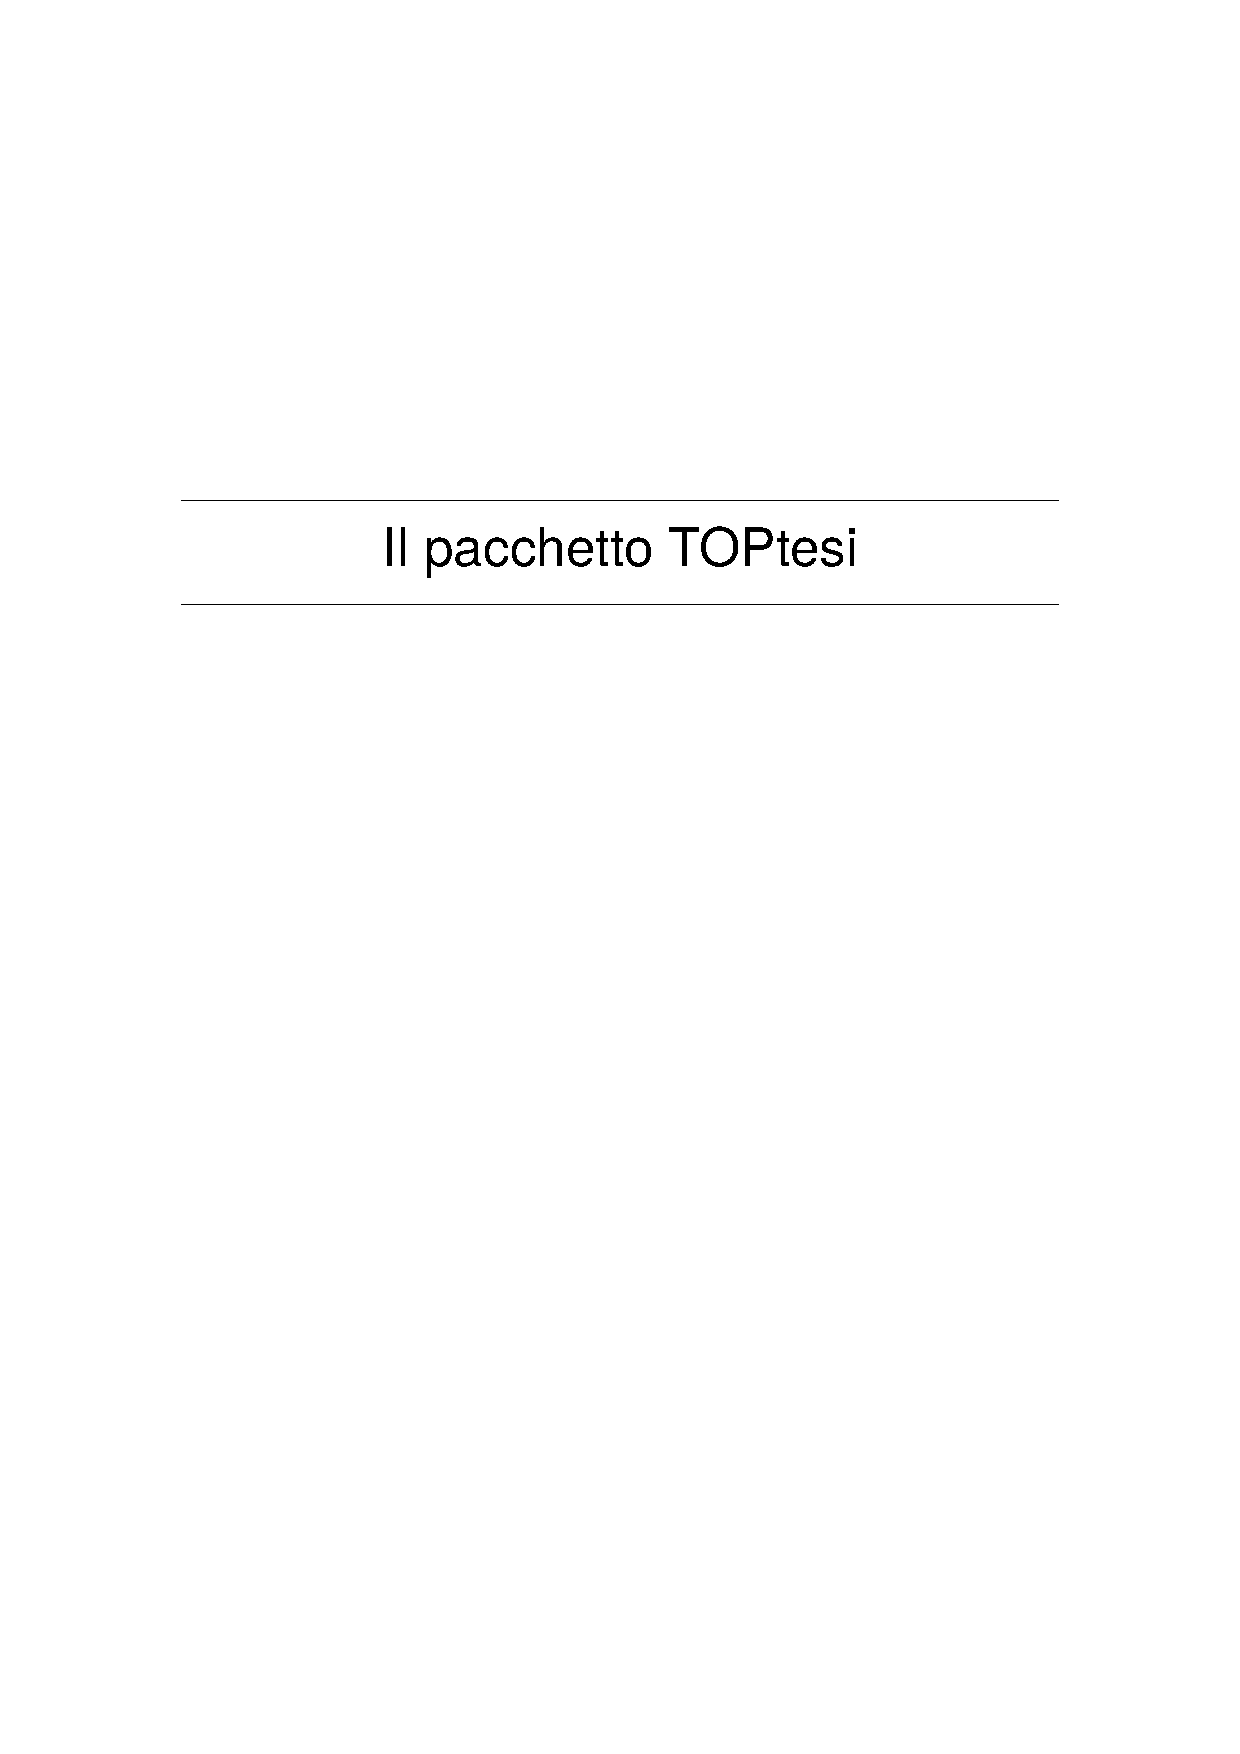
\includepdf[pages=-]{toptesi-it.pdf}
\end{document}
\end{verbatim}
e lo si affianca con il corrispondente file \file{toptesi-it-pages.xmpdata} il cui contenuto è identico al file \file{toptesi-it.xmpdata} che si sarebbe preparato per comporre l'analogo file se lo si fosse potuto comporre con \prog{pdflatex}.\par}

Il piccolo file precedente è in grado di produrre un file PDF/A perché il suo preambolo è correttamente predisposto per questo scopo; carica il pacchetto \pack{pdfpages} che serve per importare tutte le pagine (o una loro selezione) di un file PDF comunque composto, dentro il file che si ottiene elaborandolo con \textcolor{red}{\prog{pdflatex}}. Se il file \file{toptesi-it.pdf} non contiene file importati con caratteristiche incompatibili, il file PDF ottenuto risulta conforme alla norma PDF/A, ma se il file di partenza conteneva collegamenti ipertestuali, il file finale ottenuto ne è privo.

Ho usato come esempio il nome di questo stesso file di documentazione; il lettore capisce che si tratta solo di un esempio, perché questo documento si compila perfettamente in formato PDF/A senza ricorrere a questo procedimento. Ma, se per esempio, si fosse composta la tesi con un word processor e la si fosse esportata in formato PDF, questo procedimento potrebbe crearne la versione PDF/A compatibile senza sforzo e con la sola spesa di perdere i collegamenti ipertestuali interni.

Più comodamente il procedimento descritto in questo paragrafo può servire per aggiungere quanto manca, per esempio, ad una figura PDF per verificarne la conformità oppure per scoprirne le cause di non conformità, eventualmente per modificarla in modo che sia compatibile tanto da poterla includere nella tesi vera e propria. 

Per esperienza diretta, come ho già detto, quando devo convertire un file PDF comunque ottenuto io ora preferisco seguire questo procedimento che ricorre al pacchetto \pack{pdfpages} e lo consiglio vivamente rispetto ad altri metodi.

\subsubsection{Uso di \texorpdfstring{\prog*}{}{ghostscript}}

Si potrebbe anche usare \prog{ghostscript} per trasformare un file PDF in un altro conforme alla norma PDF/A. L'operazione non è semplice ed è, secondo me, mal descritta nella documentazione di \prog{ghostscript}. Se ci si sente a proprio agio con il linguaggio PostScript e si padroneggia bene il suddetto programma, si può provare. Tuttavia, pur essendomi servito di questo procedimento per diversi anni prima di poter disporre del metodo descritto nel paragrafo precedente, non lo consiglio e rimando il lettore alla documentazione di \prog{ghostscript}.

\subsubsection[Non usare \texorpdfstring{\pack}{}{pax} e \texorpdfstring{\pack}{}{pdfpages} assieme]{Non usare i due pacchetti \pack{pax} e \pack{pdfpages} assieme allo scopo di conservare i collegamenti ipertestuali}

Il pacchetto \pack{pax} è stato costruito per ridare funzionalità ai collegamenti ipertestuali contenuti in file PDF immessi completamente o in parte dentro altri file PDF. Funziona perfettamente, ma il pacchetto \pack{pdfx} non riesce a gestire le operazioni del pacchetto \pack{pax}, per cui tutte le informazioni relative ai collegamenti vengono ripristinate, ma il file complessivo non rispetta le specifiche della norma PDF/A e gli errori segnalati dalla funzione Preflight di Adobe Acrobat Pro~XI riguardano solo gli hyperlink, quando invece lo stesso file PDF ricomposto solo con l'uso di \pack{pdfx} e \pack{pdfpages} è perfettamente conforme con le norme PDF/A, anche se i suoi link non sono attivi.


\section{Verifica della conformità}

Bisogna innanzi tutto disporre degli strumenti per verificare se un file è conforme alla norma PDF/A. 

In rete ci sono siti dove viene eseguita la verifica della conformità di un file PDF con la norma del sotto"formato PDF/A-1b, ma di solito l'esito della verifica è negativo, per lo meno a me non è mai capitato che un file conforme venisse riconosciuto tale mediante le verifiche in rete.

Per verificare in modo serio la conformità ci sono alcune strade che non si escludono a vicenda.
\begin{enumerate}[noitemsep]
\item Ci si procura la versione  del programma \prog{veraPDF}; questo software nel 2016 era ancora in fase di sviluppo e per questo era considerato sperimentale; ora, 2017, il programma non è più sperimentale ma, senza escludere possibili aggiornamenti, ora è stabile. L'azienda che se ne occupa è sostenuta dalla Unione Europea proprio affinché la versione definitiva sia aperta e libera. Funziona benissimo e i suoi verdetti, secondo l'esperienza già fatta, sono praticamente sempre concordi con quelli del modulo Preflight di Adobe Acrobat Pro~XI. Questo programma è disponibile per le tre piattaforme Windows, Mac, Linux.
%
\item Si cerca in dipartimento una stazione di lavoro dove un computer sia dotato del programma commerciale {Adobe Acrobat Pro XI}; spesso i dipartimenti dispongono di licenze multiple, oppure è possibile che un ricercatore dia una mano lasciando usare un suo calcolatore sul quale è montato il software indicato. Si procede poi come indicato tra poco
%.
\item La Adobe, come molte altre imprese produttrici di software, dispone di un programma \emph{Education} che consente agli studenti e ai docenti di università e scuole secondarie superiori di acquistare i loro software a prezzi molto, molto vantaggiosi. Io come privato cittadino non mi sarei mai comprato l'Adobe Acrobat Pro~XI se non avessi avuto la possibilità di avvantaggiarmi di questa offerta vantaggiosissima ma, come professore, ho potuto farlo senza bisogno di ricorrere a nessuno per procurarmene legalmente una copia.
\end{enumerate}

\subsection{Verifica con veraPDF}
Nell'installare \prog{veraPDF} si sarà avuta attenzione di creare anche un link simbolico verso la componente \prog{verapdf-gui} che è l'applicazione da usare; il link simbolico si troverà in una cartella che sia sul percorso di ricerca dei programmi da eseguire secondo le impostazioni della propria macchina; comunque tutti i sistemi operativi consentono di impostare il percorso di ricerca attraverso i loro propri comandi o attraverso interfacce grafiche.

Fatto questo, si apre un terminale e si dà il comando \texttt{verapdf-gui}; si apre una finestra come quella che appare nella figura~\ref{fig:veraPDFinitial}.

\begin{figure}[!htb]
\begin{SDbox}{figure}[0.35]
\SDimage{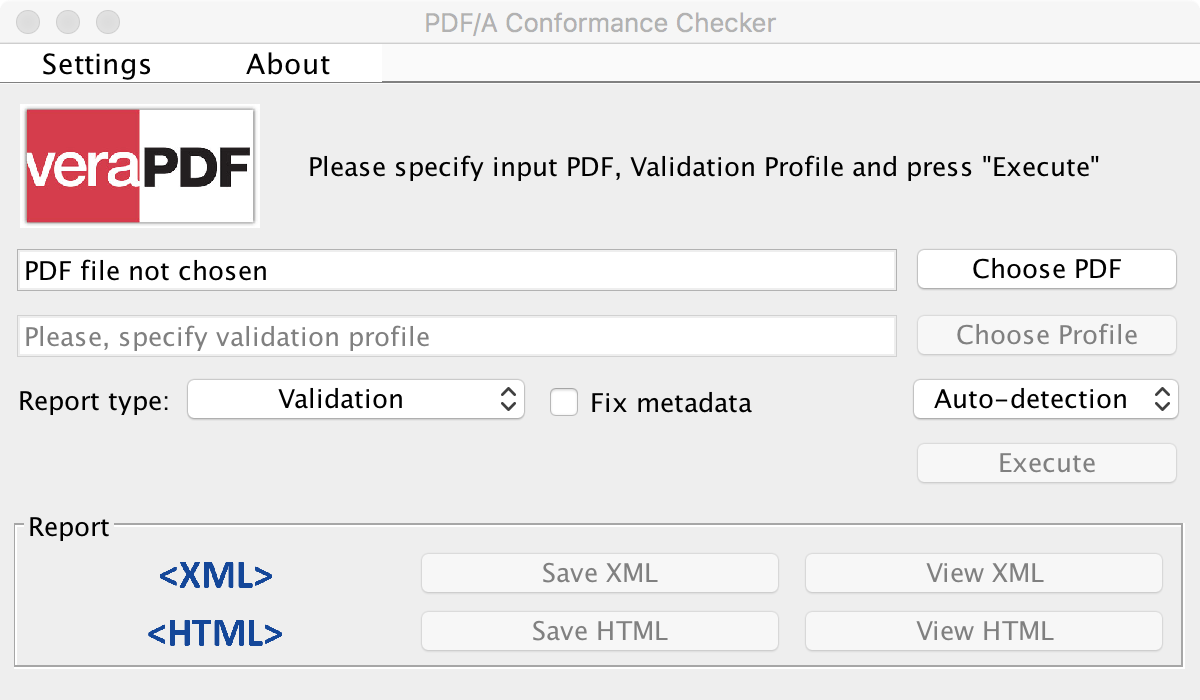
\includegraphics[width=\hsize]{VeraPDFinitial}}
\SDcaption{Finestra iniziale di veraPDF}{fig:veraPDFinitial}
\end{SDbox}
\end{figure}


In questa interfaccia grafica si clicca il bottone \fbox{Choose PDF} e nella finestra che si apre si cerca la cartella che contiene  il file da controllare. Avendolo selezionato  si ``accende'' il tasto \tasto{Execute}, cliccato il quale parte l'azione di verifica, che dura diversi secondi; finita la verifica, a seconda dell'esito, nella riga allo stesso livello del tasto \tasto{Execute} appare una scritta verde che segnala la conformità del file, oppure na scritta rossa che ne segnala la non conformità, come appare nelle due schermate della figura~\ref{fig:veraPDFesito}.

\begin{figure}[!htb]
\centering
$\vcenter{\hsize=0.7\textwidth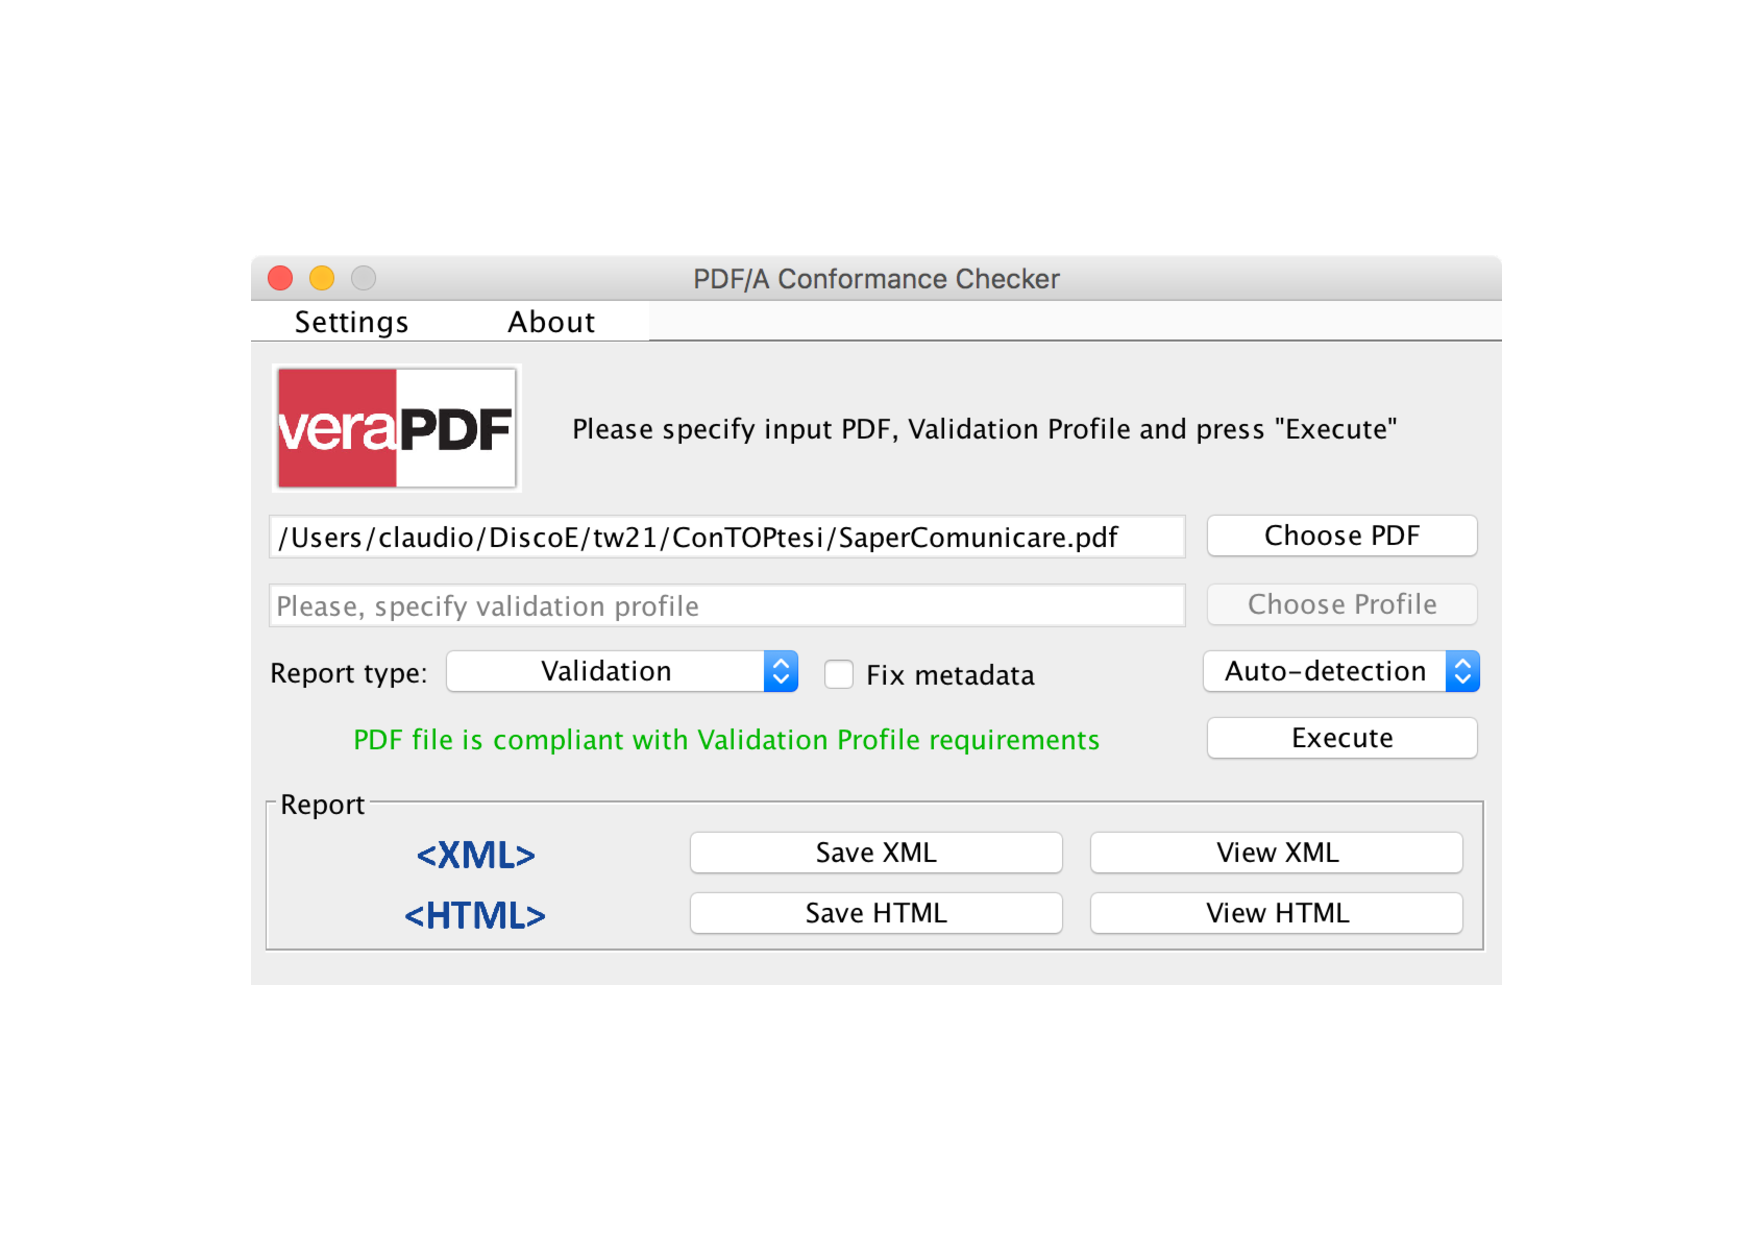
\includegraphics[width=0.7\textwidth]{veraPDFconformance}}$\qquad\setbox0\hbox{\((a)\) esito positivo}\parbox{\wd0}{\box0}
\bigskip

$\vcenter{\hsize=0.7\textwidth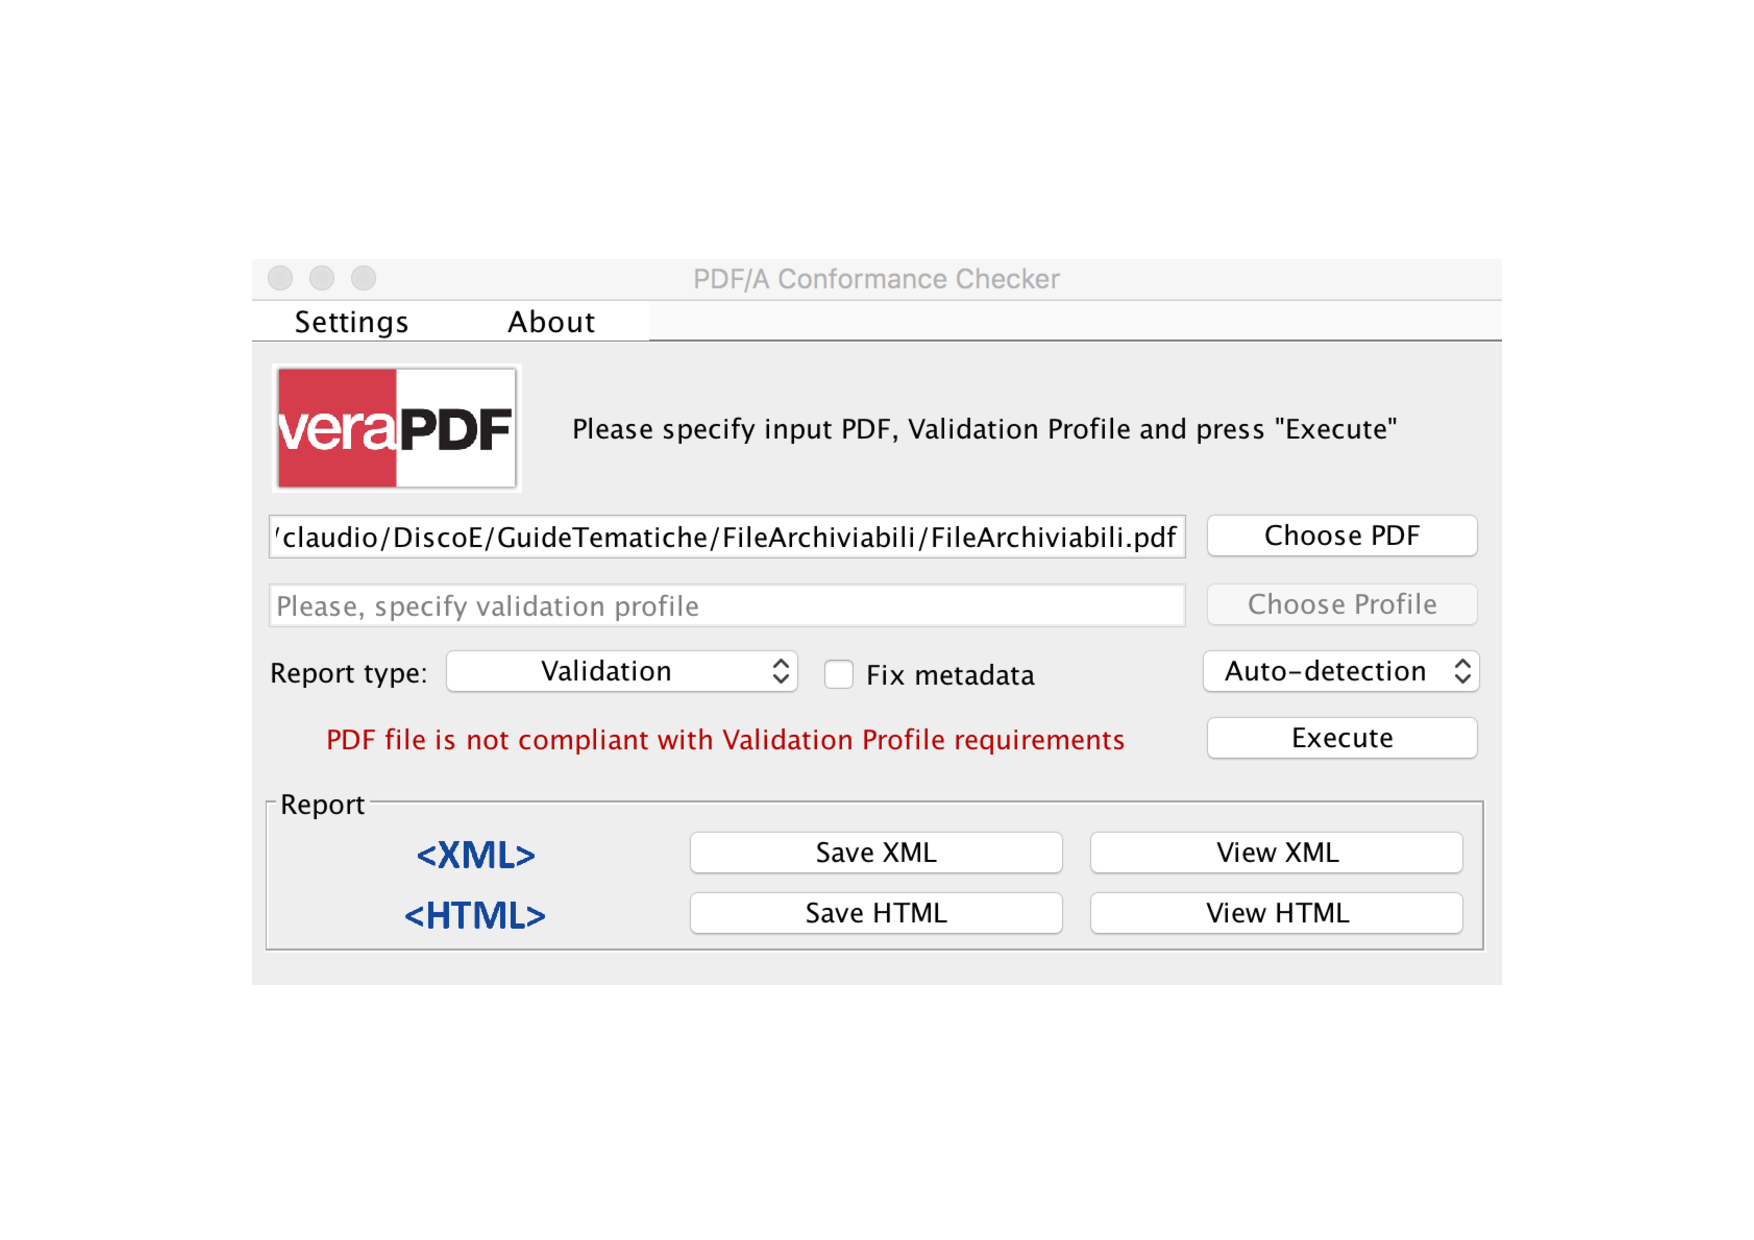
\includegraphics[width=0.7\textwidth]{veraPDFnoconformance}}$\qquad\setbox0\hbox{\((b)\) esito negativo}\parbox{\wd0}{\box0}
\caption[Verdetto dell'analisi di veraPDF su due file]{Verdetto dell'analisi di veraPDF su due file}\label{fig:veraPDFesito}
\end{figure}

{\tolerance=3000
Qualunque sia l'esito conviene visualizzare ed eventualmente salvare il verdetto cliccando sui tasti \fbox{View XML} e/o \fbox{Save XML}, oppure sui corrispondenti tasti~HTML. Se il verdetto è positivo, quanto si stampa può valere come certificazione di conformità; se l'esito è negativo il rapporto contiene una succinta spiegazione dei motivi per i quali il file non è conforme.\par}



\subsection{Verifica con Preflight}

Disponendo di Adobe Acrobat Pro XI, si apre il file PDF, si va nella voce di menù \textsf{Edit} e si sceglie l'opzione \textsf{Preflight}; nella finestrina che si apre si sceglie la voce \textsf{PDF/A compliance} e sotto questa la voce \textsf{Verify compliance with PDF/A-1b}; poi si clicca sul bottone \textsf{Analyse}; dopo pochi secondi si apre una seconda finestrina dove appare il risultato dell'analisi. Se il risultato è positivo il file è definitivamente pronto come conforme alla norma PDF/A-1b. 

Se invece l'analisi indicasse errori, bisogna provvedere a correggerli; è vero che nella stessa finestrina c'è anche il bottone \textsf{Analyse and fix}, ma l'operazione di ``aggiustamento'' di solito riesce a correggere errori molto veniali, quindi con i programmi di composizione del sistema \TeX (col quale non si compiono errori veniali) questo aggiustamento è raro che abbia successo. Ma non bisogna dimenticare che questo genere di piccoli errori spesso si presentano quando si importano file esterni; quindi tanto vale, invece, selezionare nella finestra di dialogo di Preflight la funzione Fixup; che parte e richiede con che nome si vuole salvare il file ``difettoso''; si può tranquillamente specificare di sovrascrivere il file da sistemare; fra le altre operazioni che Fixup può fare c'è anche quella di modificare il profilo di colore dei file che ne hanno uno errato, e questa, fra le altre è una operazione da fare piuttosto spesso quando si importano file esterni. L'ho dovuto fare anche con questo file di documentazione a causa di alcune figure create da me stesso per le quali non avevo controllato che avessero il profilo di colore corretto, cioè~RGB.

\subsection{Correzione degli errori}

Bisogna avere pazienza e cercare di leggere con attenzione i messaggi di diagnostica che \prog{veraPDF} o \textsf{Preflight} producono. Se mancano i metadati e/o il profilo di colore, significa che il file non è stato prodotto con le procedure descritte nei paragrafi precedenti.

Gli errori che restano sono di solito dei tipi seguenti.
\begin{enumerate}[noitemsep]
\item Se è stato specificato un profilo di colore CMYK (celeste, lilla, giallo, nero) si è fatto un errore nello specificare il profilo di colore oppure si è inserita un'immagine a colori che è colorata con lo schema CMYK. Nel primo caso è bene verificare di avere specificato il profilo giusto. Nel secondo caso bisogna convertire il profilo di colore mediante qualsiasi programma di fotoritocco; segnalo il programma aperto e libero GIMP (GNU Image Management Program), disponibile per le tre piattaforme più comuni e i sistemi operativi Mac, Windows e Linux. Esso è in grado di aprire immagini in ``qualsiasi'' formato bitmapped o vettoriale, di elaborarne il file secondo i desideri dell'utente, per poi salvarlo in qualsiasi formato bitmapped, ma non nei formati vettoriali.
%
\item Alcuni font hanno glifi di larghezza nulla, fra questi ci sono almeno due glifi della famiglia matematica \texttt{cmsym}; \pack{toptesi} provvede già da solo a sostituire questi glifi con altri simili o con disegni, in modo da correggere l'errore; tuttavia questi glifi potrebbero essere presenti in alcuni dei file importati.
%
\item Alcune figure sia raster (a cui siano state sovrapposte legende testuali con caratteri vettoriali) sia vettoriali (che contengono legende testuali) possono mancare dell'inclusione dei font; per cui quando queste immagini vengono immesse nel file PDF che si vorrebbe conforme alla norma, questa conformità viene a mancare. Se si sono prodotti personalmente tali file da includere, bisogna avere cura di far sì che tutti i glifi dei font usati nel file da includere siano essi stessi inclusi direttamente; esattamente com ho fatto con i loghi \GuIT\ e \MP\ di cui ho detto prima. Purtroppo questo è un caso molto frequente; quindi capita sovente di dover procedere alla correzione di questo genere di file.

Per le figure con legende testuali, basta convertire l'intera figura nel formato \file{.png} (se contiene disegni al tratto e purché non contenga trasparenze) oppure \file{.jpg} se contiene colori sfumati), e il gioco è fatto. 

Ma se si vuole mantenere la natura vettoriale si potrebbe usare il programma gratuito \prog{Inkscape} che è in grado di aprire file vettoriali (PDF, EPS, PS) e di trasformarli in file con le estensioni vettoriali, avendo trasformato nel contempo i caratteri nelle loro outline, cioè nei disegni dei contorni dei glifi, riempiti dello stesso colore che avevano quei glifi nella figura originale. Spesso questa trasformazione va a buon fine. 

Come esperienza personale ritengo che sia opportuno convertire ogni figura vettoriale con i glifi sostituiti dai loro contorni, solo nel formato EPS, che non gestisce le trasparenze, che sono invece gestite dal formato \file{.pdf}. In questo modo i tre programmi che ci interessano, \prog{pdflatex}, \prog{xelatex} e \prog{lualatex}, sono tutti e tre in grado di ricevere figure in formato \file{.eps}, e di incorporarlo nel file PDF in uscita. In questo modo si è sicuri di poter evitare le trasparenze, che sono vietate con lo standard PDF/A-1b. Alternativamente si riapre il file \file{.eps}  sempre cn \prog{Inkscape} e lo si salva in formato \file{.pdf}; il file \file{.eps} non conteneva trasparenze, quindi nemmeno il nuovo file \file{.pdf} ne contiene.
\end{enumerate}


\subsection{Considerazioni sulla verifica}

Come si vede, dunque, la produzione di un file conforme alla norma PDF/A non è una operazione semplice e senza disporre di Adobe Acrobat Pro XI o  di VeraPDF si consuma molto tempo per ricorrere a postazioni di lavoro esterne, dovendo chiedere favori a laboratori o ad altre persone. Però se si osservano le indicazioni di questo paragrafo, è possibile che il file della tesi sia conforme alla norma fin dal primo momento. Questa stessa guida è stata prodotta con questo tipo di procedimenti; io sono avvantaggiato per la verifica perché dispongo personalmente di entrambi i software descritti nei paragrafi precedenti. Ma, appunto, questo mio privilegio mi ha permesso di sviluppare una certa esperienza e di formulare i consigli che ho indicato nei paragrafi indicati, grazie alle soluzioni che sono riuscito a trovare nei numerosi file che ho prodotto in modo conforme alla norma. Non sono consigli infallibili e completi per risolvere qualunque problema di conformità, tuttavia ne risolvono molti e quasi sempre il procedimento ha successo. 

\chapter{I comandi specifici introdotti da \textsf{TOPtesi}}\label{cap:comandispecifici}

\section{Introduzione}

I comandi specifici introdotti da \textsf{TOPtesi} si aggiungono a
tutti quelli definiti da \LaTeX e dalla sua classe standard
\class{report}; mentre questi sono tutti in inglese o sono
abbreviazioni inglesi, i comandi introdotti da \textsf{TOPtesi} sono
prevalentemente in italiano o sono abbreviazioni italiane.

Questi comandi sono di diverse categorie; alcuni si possono usare solo in modo matematico altri solo in modo testo; alcuni solo nel preambolo, alcuni hanno senso solo durante la composizione del testo; alcuni servono solo per il frontespizio. Essi saranno descritti nei paragrafi seguenti.

\section{Le opzioni}
La classe \class{toptesi} accetta diverse opzioni nel
comando di dichiarazione della classe; negli esempi acclusi al pacchetto ne sono state usate diverse, ma qui forse vale la pena di elencarle tutte, senza ripetere le opzioni già definite per la classe \class{report}.

\begin{description}[noitemsep]\def\Item[#1]{\item[\normalfont\opt{#1}]}
\Item[chapterbib] Si raccomanda all'utente di non farne uso; esiste ancora per compatibilità con il passato. 

Servirebbe per specificare che si desidera la composizione della bibliografia alla fine di ogni capitolo; la bibliografia va composta a mano; se si desidera comporla con \textsc{Bib\TeX} si invochi invece il pacchetto \texttt{chapterbib.sty} con il solito comando \cs{usepackage}. Si abbia cura di leggere attentamente la documentazione di quel pacchetto. Alternativamente si può usare il pacchetto \pack{biblatex} (con la bibliografia da elaborare con il programma esterno \prog{biber}); bisogna specificargli opportune opzioni e si possono comporre direttamente bibliografie distinte per capitoli; si legga con attenzione la documentazione di \pack{biblatex}. Va da sé che l'uso di \pack{biblatex} con la gestione del database mediante \prog{biber} è molto più efficace e professionale della bibliografia gestita con questa opzione. %
\Item[classica] È un valore che può essere specificato alla chiave \chiave{stile} mediante l'opzione \chiave{stile}{classica}; l'alternativa è quella di non specificare niente, perché l'opzione \chiave{stile}{standard} è quella di default. Per compatibilità con il passato esiste ancora l'opzione \chiave{stile}{trieste}, che ricorda i vecchi tempi quando questo stile era stato definito per le tesi umanistiche dell'università di Trieste; se ne scoraggia l'uso. Serve per usare delle denominazioni un po' diverse dei comandi e per dare una forma diversa al loro contenuto; il frontespizio ne viene un poco modificato con un look più adatto alle tesi in discipline classiche. Si veda la tabella~\ref{tab:front5} per i comandi disponibili quando questa opzione è attivata.
%
\Item[cucitura] La chiave \chiave{cucitura} di default imposta lo spostamento della gabbia di stampa verso l'esterno; si possono specificare opzioni da \chiave{cucitura}{5mm} fino ad un massimo  \chiave{cucitura}{10mm}; di default, senza specificare nemmeno la chiave \chiave{cucitura}, lo spostamento della gabbia del testo verso l'esterno della pagina è nullo; se si specifica l'opzione senza un valore, questo viene assunto pari a 7\unit{mm}; si raccomanda di non esagerare e in particolare si raccomanda di non usare questa opzione per impostare un margine interno molto più grande di quello esterno. Serve per spostare il blocco del testo verso l'esterno quando si teme che la piegatura delle pagine verso il centro del fascicolo rilegato possa impedire la lettura agevole delle parole vicino al margine interno. Con legature eseguite bene, questa correzione non è necessaria; si ritiene che possa essere utile solo quando la tesi cartacea viene spillata.
%
\Item[corpo]  La chiave \chiave{corpo} serve per  impostare il corpo normale per il documento; se si non si specifica nulla o si specifica questa chiave senza nessun valore, il corpo normale viene impostato al valore di 10\unit{pt}; altrimenti si può specificare l'opzione da \chiave{corpo}{9.5pt} fino a \chiave{corpo}{14.5pt}. Internamente qualunque valore intero o fratto, sempre accompagnato dall'unità di misura, imposta il corpo normale secondo le stesse progressioni usate dalle impostazioni di ogni classe standard; ma per i corpi maggiori di 10\unit{pt} viene usata una progressione geometrica di ragione $1.2$, mentre per i corpi inferiori viene scelta una progressione aritmetica proporzionale a quella delle classi standard. Per tesi normali il corpo  di 9.5\unit{pt} rappresenta il minimo assoluto per non rendere troppo faticosa la lettura continua del testo; per i corpi maggiori, 12.5\unit{pt} è il massimo ragionevole per la lettura da parte di adulti senza problemi di vista; corpi fino a 14.5\unit{pt} sono utili per testi che contengano molti segni di mark-up filologico che aumentano abbastanza l'altezza e la profondità delle righe che contengano questo genere di marcature. L'esperienza ha indicato il valore di 14\unit{pt} come adatto alla composizione di simili testi con marcatura filologica. Va da sé che usando corpi così grandi la giustificazione del testo e la composizione dei titoli può diventare problematica.
%
\Item[autoretitolo] {\leavevmode\tolerance=9999 
Questa opzione funziona solo se viene
specificata anche l'opzione \chiave{stile}{classica}; se la si inserisce senza specificare questa opzione, non succede nulla di male, semplicemente la classe informa di aver trovato delle opzioni che né lei né altri pacchetti hanno usato. Serve per comporre la
testatina di sinistra sulle pagine pari con l'indicazione del
candidato e del titolo della tesi. È ovvio che il titolo della
tesi con questa opzione deve essere molto breve, ed è per questo
che è  stato messo a disposizione dello studente l'argomento
facoltativo del comando \cs{titolo} che consente di specificare
un titolo di tre o quattro parole (brevi) ma di senso compiuto,
che possa sostituire il titolo normale, specialmente se questo è
un po' lungo.\par}
%
\Item[oldstyle]  Anche questa opzione è adatta a funzionare con  \chiave{stile}{classica}; serve per scrivere i numeri 
delle pagine con le cifre minuscole o all'antica, cioè  con segni 
di altezze e profondità diverse; si confrontino le cifre minuscole \oldstylenums{123456\discretionary{}{}{}7890}  con quelle maiuscole  1234567890.
%
\Item[numerazioneromana] Questa opzione è inserita più per retrocompattibilità che per altro. Nelle versioni precedenti di \TOPtesi la parte iniziale aveva le pagine numerate con numeri romani; col primo capitolo automaticamente cominciava la ``main matter'', il corpo principale della tesi, e la numerazione ricominciava da~1 con cifre arabe. Questo modo di procedere era giustificato quando la tipografia si serviva di caratteri metallici, con i quali prima si componevano le pagine del corpo principale e solo quando queste erano state completate con la loro numerazione in cifre arabe a partire da~1, allora si potevano comporre gli indici, le introduzioni, le presentazioni e quant'altro andasse composto nella parte iniziale, con numerazione romana per non dover cambiare la numerazione della parte principale. Con la tipografia elettronica questo artifizio non ha più motivo di essere ancora usato. Tuttavia graze a questa opzione si può ripristinare il comportamento delle versioni precedenti; oppure si può usare questa opzione per dare un tocco di ``antichità'' alla tesi.
%
\Item[libro] Questa opzione permette di comporre la tesi con i margini esterno e interno diversi, precisamente nel rapporto $3:2$ con il margine esterno più largo di quello interno, conformemente alla tradizione tipografica. Lo specchio di stampa resta invariato rispetto a quando i margini sono uguali; questo cambiamento dei margini consente il funzionamento della variazione della correzione di legatura prodotto dal valore assegnato alla chiave \chiave{cucitura}. Tuttavia se l'utente vuole stamparsi la tesi con i margini diversi secondo la tradizione, vuol dire che ci tiene a che il “libro” della tesi sia confezionato bene; quindi se lo legherà o se lo farà rilegare con le segnature cucite e con una copertura rigida, lasciando perdere la confezione più economica col dorso incollato.
%
\Item[pdfa] Prima della distribuzione di \TeXLive 2016 il pacchetto \pack{pdfx} doveva essere caricato dalla classe, non nel preambolo del documento come si può fare ora con la distribuzione aggiornata di \TeXLive. Per compatibilità con il passato, l'opzione esiste ancora, ma produce solo un avviso e non carica \pack{pdfx}.
%
\Item[tipotesi] La chiave \chiave{tipotesi} serve per esprimere delle opzioni che riguardano il tipo della tesi, almeno il modo di comporre il suo frontespizio; essa accetta diversi valori; se non si specifica l'opzione o non si specifica nessun valore, per il frontespizio viene usato il modulo \pack{topfront}. I valori che si possono specificare sono indicati nella tabella~\ref{tab:tipotesi}
\end{description}

\afterpage{%
\begin{table}[p]\centering
\caption[Valori particolari per la chiave \texttt{tipotesi}]{Valori particolari per la chiave \chiave{tipotesi}}\label{tab:tipotesi}
{\small
\begin{tabularx}{\linewidth}{llX}
\toprule
Opzione & Modulo caricato & Scopo \\
\midrule
nessuna & \pack{topfront} & {Serve per comporre la tesi usando il modulo di default, che essendo di tipo generale, può risultare difficile da usare\par} \\
\chiave{tipotesi} & \pack{topfront} &{Come nel caso precedente\par}\\
\chiave{tipotesi}{triennale}& \pack{toptesi-triennale} & {Serve per comporre il frontespizio del lavoro finale del primo ciclo triennale universitario\par}\\
\chiave{tipotesi}{monografia}& \pack{toptesi-triennale} & {Come nel caso precedente \par}\\
\chiave{tipotesi}{magistrale}& \pack{toptesi-magistrale} & {Serve per comporre il frontespizio della tesi del secondo ciclo biennale universitario che porta al diploma di laurea magistrale; vale anche per i corsi di studio a ciclo unico \par}\\
\chiave{tipotesi}{dottorale}& \pack{toptesi-dottorale} & {Serve per comporre il frontespizio di una dissertazione dottorale generica, e diversa da quella dalla Scuola di Dottorato del Politecnico di Torino \par}\\
\chiave{tipotesi}{scudo}& \pack{toptesi-scudo} & {Serve per comporre il frontespizio delle tesi dottorali presso la Scuola di Dottorato del Politecnico di Torino \par}\\
\chiave{tipotesi}{frontespizio}& \pack{frontespizio} & {Usa un pacchetto esterno e i suoi specifici comandi per comporre il frontespizio \par}\\
\chiave{tipotesi}{secondaria}& \pack{toptesi-sss} & {Serve per comporre il frontespizio per la tesina dell'esame di maturità \par}\\
\chiave{tipotesi}{custom}& nessuno & {Richiede l'intervento attivo dell'utente. \par}\\
\bottomrule
\end{tabularx}}
\end{table}}


\section{Comandi di tipo generale}
I comandi di tipo generale si possono usare in ogni contesto, in
particolare alcuni sono fatti per essere usati sia in modo testo 
sia in modo matematico. Essi sono raccolti nella 
tabella~\ref{tab:generale}.

\goodpagebreak[6]

\afterpage{%
\begin{table}[p]%\def\V{\rule{0pt}{2.5ex}}
\caption{Comandi di tipo generale}\label{tab:generale}
\centering \cambiacorpo{9.5}%
\begin{tabular}{llp{.26\textwidth}p{.30\textwidth}}
 \toprule
 Comando  & Default   & Scopo     & Esempio d'uso  \\[.5ex]
 \midrule
 \cs{interlinea}\Arg{...} &
                    1.0    & Modifica l'argomento di
                             \cs{linespread}\newline \textcolor{red}%
                             {NON usare se non
                              costretti con la forza!}\newline Modo 
                              testo  
                                 &\raggedright
                                  \cs{interlinea}\Marg{1.05} \newline
                                   oppure \newline
                                   \Bambiente{interlinea}% 
                                   \Marg{1.05}\newline
                                   \dots\newline
                                   \Eambiente{interlinea}\newline
                                  Vedi annotazioni 
                                  sull'interlinea nel testo\cr
\cs{ohm}         &         & Omega ``diritto''\newline
                             Modi testo e matematico    &  
                             \texttt{45\string\ohm}\\ 
\cs{ped}\Arg{...}& nessuno & Pedice in tondo\newline
                             Modi testo e matematico   
                             & \texttt{\string$V\relax
                             \string\ped\{eff\}\string$} \\
\cs{ap}\Arg{...}& nessuno & Apice in tondo\newline
                             Modi testo e matematico   
                             & \texttt{\string$M\relax
                             \string\ap\{T\}\string$} \\
\cs{unit}\Marg{...}&nessuno & Unità di misura in
                             tondo unite al numero\newline
                             Modi testo e matematico    
                             & \texttt{15\string 
                             \unit\Arg{k\string\ohm}}  \\
\cs{gei}       &           & Unità immaginaria in
                             tondo \newline
                             Solo modo matematico       
                             & \texttt{\string$
                             \string\eu\string^\string{\string\gei
                             \string\omega\ t\string}\string$} \\
\cs{eu}        &           & Numero ``e'' in tondo\newline 
                             Solo modo matematico  
                           & \texttt{\string$
                           \string\eu\string^\Arg{\string\gei
                           \string\omega\ t}\string$} \\
\cs{gradi}     &           & circoletto alzato\newline  Modo testo e
                             matematico  & \texttt{27\string\unit
                             \Arg{\string\gradi\ C}} \\
\cs{listing}\Arg{...}&
                 nessuno    & Listato di un programma in caratteri 
                             typewriter   & \texttt{\string\listing
                             \string{toptesi.tex\string}}\\
\cs{blankpagestyle}\Arg{...}&plain	&\raggedright Impostazione dello stile della 
                             pagina eventualmente emessa da 
                             \cs{cleardoublepage} quando deve 
                             passare ad una pagina dispari in 
                             composizione fronte retro
                                                     	& \cs{blankpagestyle}\Arg{empty}\\
\cs{goodpagebreak}\Oarg{...}
               & 4          & Inserisce un fine pagina condizionale;
                              l'argomento facoltativo serve per 
                              specificare il numero di righe 
                              necessarie prima del fine pagina 
                              condizionale 
                            &\cs{goodpagebreak}\Oarg{5}\\
\amb{SDbox}\Marg{...}& \Marg{} & Figura con didascalia accanto
                            & Vedi nella pagina~\pageref{pag:SD}\\
\cs{captionof} & nessuno    & Permette di assegnare una didascalia
                              ad oggetti non inseriti dentro un 
                              ambiente mobile
                            & \cs{captionof}\Marg{figure}%
                              \discretionary{\%}{}{}%
                              \Marg{Didascalia}\\[.5ex]
\bottomrule
\end{tabular}
\end{table}}

\subsubsection{Il comando \texorpdfstring{\cs}{}{interlinea} e l'ambiente corrispondente}
{\tolerance=6000 Vale la pena di commentare sull'uso dell'ambiente \amb{interlinea} e del comando \cs{interlinea}.
Il primo confina il suo effetto all'interno dell'ambiente da lui
stesso formato; il secondo agisce come una dichiarazione che resta
in vigore finché  una dichiarazione contraria non ne modifichi il
valore.
\textcolor{red}{Tuttavia sia l'ambiente sia il comando non dovrebbero essere mai usati!}\par}

La composizione tipografica non ha nulla a che vedere con la composizione  dattilografica. Quest'ultima si faceva con mezzi avanzati per l'epoca, ma oggi quei mezzi sono del tutto obsoleti; le poche macchine da scrivere meccaniche o elettromeccaniche che esistono ancora fuori da qualche museo, vengono usate per riempire formulari o compilare le  informazioni sui documenti cartacei che sopravvivono alla invasione delle carte plastificate; ma tolti gli usi burocratici non mi viene in mente nessun altro uso degno di nota.

La composizione tipografica esige un perfetto equilibrio fra il corpo del font usato e la distanza fra le righe su cui sono appoggiati i caratteri di due righe di testo consecutive; questa distanza prende il nome tecnico di \emph{scartamento} o \emph{avanzamento di riga}, ma spesso viene chiamato impropriamente \emph{interlinea}; questo scartamento a seconda del font in uso può essere dal 10\% al 20\% maggiore del corpo del font usato.

Questa documentazione è scritta in corpo 12\,pt e lo scartamento è di 14,5\,pt; si dice che questo testo è composto in corpo 12/14,5.

\begin{interlinea}{1.05}
L'interlinea, come suggerisce il nome, era originariamente lo spazio aggiuntivo da inserire fra una linea e l'altra; quando la composizione tipografica era eseguita con font metallici, l'interlinea era la striscia di metallo che veniva interposta fra una riga di caratteri e la successiva. Il comando \cs{interlinea} e l'ambiente corrispondente hanno pertanto dei nomi che si rifanno alla tipografia tradizionale, ma vengono usati come in dattilografia. In effetti l'argomento del comando e dell'ambiente serve solo come fattore moltiplicativo dello \emph{scartamento}; porre questo fattore al valore \texttt{1.05} vuol dire moltiplicare lo scartamento per 1,05 portandolo quindi dal valore di 14.5\,pt al valore di 15,5225\,pt. Questo capoverso è  composto con questo fattore impostato con l'ambiente \amb{interlinea} e, nonostante si tratti solo di un aumento del 5\% dello scartamento, l'occhio lo percepisce in modo più grande di quanto non faccia pensare il suo piccolo valore.
\end{interlinea}

L'avanzamento di default scelto per i caratteri in uso è
l'avanzamento otticamente ottimale; se si desidera usare un font
diverso da quello di default, si potrebbe, per esempio, invocare il
pacchetto \Font{newpxtext} per usare il Palatino esteso come font
di testo. Siccome questo font a pari corpo ha le minuscole
più grandi di quelle dei font di default, potrebbe
essere una idea sensata quella di sperimentare con diversi valori
del fattore di \amb{interlinea}, ma poi si scoprirebbe che
questo fattore differirebbe di pochi centesimi dall'unità e quindi
ci sarebbe da domandarsi se ne valga la pena.

Se proprio si vogliono stampare su carta delle bozze scritte  abbastanza larghe per potervi inserire le correzioni e le annotazioni 
a mano, allora si imposti il fattore di \amb{interlinea} al massimo a
\texttt{1.5}, ma quando si stampa la bella copia, la versione finale,
ci si ricordi di re-impostare per \amb{interlinea} il valore unitario
di default.

Tra l'altro non si vuole mica usare l'espediente di un grande fattore
di interlinea solo per rimpolpare una tesi dal volume modesto? Esso
sarebbe un espediente talmente puerile che sarebbe scoperto al primo
sguardo. Ricordate che alcune tesi svolte al Politecnico di Torino all'inizio degli anni 20  del XX secolo non superavano le 30~pagine dattiloscritte o scritte a mano (!), ma ricevettero la dignità di stampa\footnote{Una era del candidato Carlo Alberto Castigliano e vi veniva enunciato il teorema di Castigliano; un'altra era di Placido Cicala e vi si svolgeva la teoria delle volte sottili, teoria che gli strutturisti considerano assolutamente fondamentale ancora oggi.}; le si sta studiando ancora oggi dopo quasi un secolo!

\subsubsection{La misteriosa pagina bianca}
Vale la pena di commentare il misterioso comando \cs{blankpagestyle}. Quando si compone fronte e retro senza usare l'opzione di classe \opt{openright}, i capitoli vengono sempre aperti nelle pagine di destra, cioè nelle pagine dispari. Per fare questo il comando \cs{chapter} agisce eseguendo subito il comando \cs{cleardoublepage} che, fra le altre cose, controlla se la nuova pagina su cui scrivere il titolo del capitolo sia dispari. Se non lo fosse provocherebbe la stampa di una pagina ``bianca''; bianca nel senso che non contiene testo ma contiene la testatina e il piedino.

Fino alla versione 0.62 di \TOPtesi,  questa eventuale pagina bianca prima dell'apertura di un nuovo capitolo conteneva la testatina e il piedino; d'accordo nel piedino c'è solo il numero della pagina, e ci può stare, ma nella testatina rimaneva il titolo del capitolo precedente: tipograficamente molto antiestetico ed errato. Da molti annni questa pagina bianca viene composta di default solo con il piedino che, ricordiamo, contiene solo il numero della pagina. Alcuni preferiscono che questa pagina bianca sia davvero vuota e non contenga nemmeno il piedino; ecco, in questo caso basta specificare:
\begin{flushleft}\ttfamily
\cs{blankpagestyle}\{empty\}
\end{flushleft}
e il problema è risolto. Volendo si potrebbe specificare il nome di qualunque altro stile di pagina già definito ma, ad essere franchi, non vedo alternative fra i due stili \texttt{plain} e \texttt{empty} rispetto agli altri stili che contengono sempre le testatine, eventualmente ridotte al solo loro filetto. 

Se lo si vuole usare, consiglio di farlo subito dopo \Bambiente{document}.

Se invece si desidera lasciare il valore di default a \texttt{plain} e usare saltuariamente un altro stile, si usi esplicitamente il comando \cs{cleradoublepage} specificando lo stile desiderato come argomento facoltativo, per esempio:
\begin{verbatim}
\cleardoublepage[empty]
\end{verbatim}

Riassumendo: per una pagina veramente vuota sempre e in ogni caso; si specifichi
\begin{verbatim}
\blankpagestayle{empty}
\end{verbatim}
subito dopo \Bambiente{document}. 

Se si desidera una pagina vuota saltuariamente si espliciti \cs{cleardoublepage} con l'argomento facoltativo \texttt{empty}. Se si desidera modificare lo stile della pagina bianca quando il comando \cs{cleardoublepage} è emesso da uno specifico comando \cs{part} o uno specifico comando \cs{chapter} si usi \cs{cleardoublepage}\texttt{[empty]} \emph{subito prima} di quel comando di sezionamento. 

\subsubsection{L'ambiente \texorpdfstring{\amb*}{}{SDbox}}
Un nuovo ambente \amb{SDbox}\label{pag:SD} è disponibile per comporre una figura o una tabella o qualunque altro contenuto, con una didascalia accanto invece che sotto come avviene con gli ambienti normali. Richiede un primo argomento costituito dal nome del tipo di oggetto da gestire; vedi sotto.

Si tratta di un ambiente non flottante, per cui può apparire in mezzo al testo o anche insieme ad un altro oggetto in un ambiente flottante qualsiasi; capita, per esempio, di dover comporre una tabella di dati che si vogliono rappresentare anche con un grafico; è comodo che tabella e figura siano associati dentro lo stesso ambiente flottante in modo che rimangano sempre assieme. Il diagramma potrebbe essere dotato di una didascalia numerata con le sue spiegazioni; e qui l'ambiente \amb{SDbox} torna comodo. 

Per usare questo ambiente bisogna seguire una sintassi particolare che richiede argomenti non delimitati o delimitati in modo particolare, per cui è opportuno specificare la sintassi in modo dettagliato.
\begin{flushleft}\obeylines
\Bambiente{\meta{foat}}
\qquad\Bambiente{SDbox}\marg{tipo}\meta{asterisco facoltativo}%
      \oarg{frazione}
\qquad\qquad\cs{SDimage}\meta{comandi per l'immagine}
\qquad\qquad\cs{SDcaption}\oarg{didascalia breve}\marg{didascalia}%
     \marg{etichetta}
\qquad \Eambiente{SDfigure}
\Eambiente{\meta{float}}
\end{flushleft}
dove i vari argomenti hanno il seguente significato.
\begin{enumerate}[noitemsep]
\item
    Il \meta{tipo} indica il tipo di oggetto da presentare con la 
    didascalia accanto; deve coincidere con uno dei nomi nome degli 
    ambienti che fanno flottare gli oggetti; quindi normalmente 
    \meta{tipo} può valere ``figure'', oppure ``table'' e, se 
    sono stati definiti altri ambienti flottanti con le 
    funzionalità del pacchetto \pack{float}, i nomi di questi 
    altri ambienti. Nel seguito ci si riferirà ad ogni tale
    oggetto con la parola ``immagine'', sia essa davvero una 
    figura, o una tabella, o un algoritmo, o qualunque altro 
    \meta{tipo} che si possa etichettare con una didascalia.
\item
   L'\meta{asterisco facoltativo} va inserito dopo il \meta{tipo}. 
   Senza usare l'asterisco l'oggetto formato complessivamente
   dall'immagine e dalla sua didascalia viene composto dentro 
   una scatola larga quanto la giustezza ordinaria del testo 
   circostante; se invece si usa l'asterisco la scatola che 
   contiene l'oggetto è più larga e protrude nel margine esterno 
   occupando quasi tutto lo spazio che sarebbe destinato alle 
   note marginali; si vedano le figure~\ref{fig:logo} 
   e~\ref{fig:logo-largo}, la prima composta senza asterisco 
   e la seconda con l'asterisco. Nel seguito 
   chiameremo \emph{scatola SD} questa scatola che contiene 
   oggetto e didascalia.\footnote{Nella figura~\ref{fig:logo-largo} 
   lo spazio tra l'immagine e la didascalia è maggiore 
   di quello della figura~\ref{fig:logo}; non dipende dal fatto 
   che la scatola SD sia più larga, ma dal fatto che la didascalia 
   composta con le funzionalità di \TOPtesi si ridimensiona 
   automaticamente per non lasciare l'ultimo righino troppo corto.}
   
   \begin{figure}
      \begin{SDbox}{figure}
         \SDimage{\centering
\includegraphics[width=\hsize]{TITlogoCropped}}
         \SDcaption[Il logo di PoliTO (1)]{Il Logo del Politecnico di 
         Torino inserito con una didascalia a fianco}{fig:logo}
      \end{SDbox}\\[\bigskipamount]
      \begin{SDbox}{figure}*
         \SDimage{\centering
\includegraphics[width=\hsize]{TITlogoCropped}}
         \SDcaption[Il logo di PoliTO (2)]{Il Logo del Politecnico di 
         Torino inserito con una didascalia a fianco che fuoriesce 
         nel margine}{fig:logo-largo}
      \end{SDbox}
   \end{figure}
%
\item 
   L'argomento \meta{frazione} serve per definire mediante 
   un numero decimale compreso fra 0.3 e 0.7\footnote{Usare il punto, 
   non la virgola, per questi dati da dare in pasto a \LaTeX.} 
   la frazione della larghezza della scatola SD  da dedicare 
   alla didascalia; la parte restante della 
   larghezza di tale scatola viene dedicata all'immagine; in realtà 
   entrambe verranno diminuite dello spazio intercolonna per 
   lasciare una netta distinzione fra la didascalia e l'immagine. 
   Se per sbaglio venisse indicata una \meta{frazione} esterna 
   all'intervallo indicato, essa verrebbe riportata all'estremo 
   più vicino dell'intervallo. Ovviamente né la didascalia né 
   l'immagine debbono avere uno spazio orizzontale troppo piccolo
   e questo è il motivo per il quale si sono definiti dei limiti 
   all'intervallo dentro il quale deve cadere il valore di questa 
   \meta{frazione}.
\item
   I \meta{comandi per l'immagine} sono quei comandi che servono
    per generare o per importare un'immagine; possono essere 
    formati da una serie di comandi di disegno programmato (con 
    l'ambiente \amb{picture} o con gli ambienti disponibili 
    con i pacchetti \pack{tikz} o \pack{pgfplots}; possono essere
    tabelle costruite con gli ambienti \amb{tabular},
    \amb{tabular*}, \amb{tabularx}, \amb{widetable} e simili, 
    ma bisogna curare che agli ambienti di larghezza prefissata sia 
    specificata una larghezza che on ecceda la larghezza della 
    scatola; a questa ci si riferisce con il nome \cs{SDfigurewidth} 
    o con la macro del nucleo di \LaTeX \cs{hsize}; possono essere 
    formati da comandi di centratura nello spazio della 
    frazione destinata all'immagine; possono essere costituti 
    dal comando \cs{includegraphics} con le sue molteplici 
    opzioni. A questo proposito vale la pena di ribadire che lo 
    scalamento dell'immagine grafica va fatto con riferimento 
    alla larghezza destinata all'immagine; larghezza che 
    \emph{non è indicata} da \cs{linewidth} o da simili comandi 
    che si riferiscono solo al testo circostante, ma ai parametri 
    interni alla scatola destinata all'immagine, cioè la lunghezza 
    indicata con \cs{SDfigurewidth} oppure con \cs{hsize}.
\item
   La \emph{didascalia breve} è l'indicazione facoltativa da 
   usare anche con  \cs{caption} per inviare alla 
   ``lista delle figure'' un titolo sufficientemente breve, 
   e non l'intera didascalia, che spesso impegnerebbe più 
   righe; in quell'elenco bisognerebbe usare una riga sola, 
   massimo due, ma il valore `due' costituisce già una eccezione 
   alla regola.
\item
   Non occorre specificare nulla in merito alla \meta{didascalia}. 
   Si ricorda soltanto che la didascalia è fatta di tre parti; 
   il prefisso con il nome e il numero seguito da qualche 
   segno di separazione, talvolta formato solo da spazio non 
   scritto; il titolo che è generalmente una frase senza verbo 
   e che se non è seguita da altro non termina col punto finale; 
   questo invece è presente se c'è la terza parte: la descrizione 
   (facoltativa), che contiene dettagli ulteriori relativi 
   all'immagine e termina con il punto finale. Nessun comando 
   che io conosca, anche definito in altre classi o in altri 
   pacchetti distingue con argomenti diversi queste tre parti; 
   sarebbe utile ma non ne ho creato una definizione in \TOPtesi.
   
\afterpage{%
\begin{table}[!htb]
\caption[Possibilità d'uso di \cs{SDbox}]{Combinazioni possibili con le situazioni facoltative dell'uso di \cs{SDbox}}
\label{tab:SDcombinazioni}

\centering
\begin{tabularx}{\textwidth}%
							{m{0.2\textwidth} c *2{>{\centering}X}}
\toprule
\multicolumn4c{Prefisso del numero della didascalia nella scatola SD libera}   \\[0.5ex]
&&\multicolumn2c{\meta{tipo}\ap{*}} \\
\cmidrule{3-4}
        	&			& Sì										& No								\cr
\midrule
					& Sì	& uguale a \meta{tipo} o errore\ap{*}	& non numerata				\cr
 \raisebox{0.5\baselineskip}[0pt][0pt]{\meta{etichetta}}
          & No	& non numerata								& non numerata		\tabularnewline\\[0.5ex]
\midrule
\multicolumn4c{\parbox{0.95\textwidth}{\centering Prefisso del numero della didascalia nella scatola SD  dentro un ambiente \meta{float}}}   \\[0.5ex]
&&\multicolumn2c{\meta{tipo}\ap{*}} \\
\cmidrule{3-4}
       &	& \meta{tipo}${}={}$\meta{float}& \meta{tipo}${}\ne{}$\meta{float}\cr
\midrule
        	& Sì  & uguale a \meta{float} 	&  uguale a \meta{tipo} o errore\ap{*} 	\cr	
\raisebox{0.5\baselineskip}[0pt][0pt]{\meta{etichetta}}
				& No	& non numerata								& non numerata						\tabularnewline[2ex]
\multicolumn4{p{0.95\textwidth}}{\footnotesize\ap{*} Si manifesta un errore se \meta{tipo} è diverso dal nome di qualsiasi ambiente flottante definito.}\\
\bottomrule
\end{tabularx}
\end{table}}
%
\item
   Il terzo argomento del comando \cs{SDcaption} termina con 
   l'\meta{etichetta} da assegnare alla figura; questa etichetta 
   è quella che solitamente costituisce l'argomento del comando 
   \cs{label} qui non lo si usa direttamente perché ci pensa 
   \cs{SDcaption} a usare \cs{label} al momento opportuno  e a 
   conservare l'etichetta in un dato registro perché i 
   comandi di chiusura dell'ambiente possano gestire correttamente 
   la scatola della didascalia e quella dell'immagine in modo 
   che la didascalia sia sempre verso il lato esterno della pagina; 
   questa quindi verrà composta a destra nelle pagine di destra e 
   a sinistra nelle pagine di sinistra. Componendo solo in bianca, 
   la didascalia cade sempre a destra.
\item
   Il \meta{float} (se viene usato), il \meta{tipo} e l'\meta{etichetta}
   giuocano ruoli fra loro subalterni 
   a quelli descritti sopra. Bisogna ricordare che la scatola SD 
   può contenere una didascalia numerata col suo prefisso, oppure una 
   didascalia non numerata e priva di prefisso. Se 
   l'\meta{etichetta} (facoltativa) non viene specificata la 
   didascalia non viene numerata se il \meta{tipo} non è noto; 
   se il \meta{tipo} (opzionale) viene specificato, può essere 
   anche diverso da quello dell'ambiente flottante circostante, 
   altrimenti viene assunto uguale a quello dell'ambiente 
   circostante; ancora la scatola SD non deve necessariamente 
   essere dentro un ambiente flottante. Dunque le possibilità di 
   numerare o non numerare la didascalia e con un prefisso 
   specifico sono molteplici; si veda la 
   tabella~\ref{tab:SDcombinazioni}.
\end{enumerate}

Questa lunga descrizione si è resa necessaria per consentire al lettore di usare correttamente questo ambiente; esso è molto utile quando si devono inserire delle piccole figure che altrimenti lascerebbero troppo spazio ai loro fianchi; vale anche con figure che hanno un prevalente sviluppo verticale. Non è il caso di usarlo sempre, ma solo quando il contenuto lo richiede. Vale anche, come si è già detto quando una figura con didascalia va inserita assieme ad una tabella dentro l'ambiente \amb{table}, o viceversa.

Preciso che se viene caricato il pacchetto \pack{caption}, la definizione di questo ambiente non è più disponibile perché essa fa riferimento a come è stato ridefinito il comando \cs{caption} di questa classe. Se si volessero usare ugualmente alcune figure con la didascalia a lato, si può usare il pacchetto \pack{sidecap} che ha prestazioni simili, ma con meno funzionalità rispetto a quelle qui descritte, in quanto produce solo figure (e tabelle) flottanti.

\subsubsection{Il comando \texorpdfstring{\cs*}{}{goodpagebreak}}
Qualche annotazione va fatta per il comando \cs{goodpagebreak}. Il nucleo di \LaTeX contiene il comando \cs{goodbreak} che dovrebbe impostare un consenso di eseguire un fine pagina impostando una penalità molto piccola negativa, più o meno simile a quello che fa il comando \cs{pagebreak}\Oarg{1}. In realtà questo comando nativo di Plain \TeX, conservato in \LaTeX, di fatto non funziona come ci si aspetterebbe. Il comando di questa classe, \cs{goodpagebreak} procede in un altro modo, anche perché si comporta in modo diverso se viene specificato in modo verticale o in modo orizzontale. 

Infatti in modo orizzontale inserisce d'ufficio un comando \cs{vadjust} il cui argomento vale esattamente \cs{newpage} che agisce in modo incondizionato quando la \emph{riga} che lo contiene viene scritta nel file di uscita; si dovrà porre un minimo di attenzione a fare sì che lo spazio alla fine della macro non elimini spazi interparola, né introduca spazi spuri; quando lo si usa, quindi, sarà opportuno lasciare uno spazio prima e dopo la macro, per esempio 
\begin{flushleft}\verb*|...prima \goodpagebreak di...|\end{flushleft}

Vale la pena di usare questo comando in certi casi in cui la bozza (non interlineata) mostra un salto pagina prima dell'ultima riga di un capoverso, cioè quando viene prodotta una riga vedova; quando si corregge la bozza si cerca il testo della riga prima di quella vedova e si inserisce la macro fra due parole qualsiasi di quel testo. È evidente che se si modifica il capoverso e non c'è più bisogno del salto pagina incondizionato, bisogna cancellare la macro da quella posizione.

In modo verticale, invece, viene calcolata la differenza fra le lunghezze \cs{pagegoal} e \cs{pagetotal}; la prima corrisponde più o meno a \cs{textheight} diminuita dello spazio riservato alle note in calce e del loro spazio di separazione dal testo; è insomma l'obbiettivo per raggiungere la giusta altezza del testo; la seconda lunghezza è la lunghezza netta del testo raggiunta fino a quel momento; se questa differenza è \emph{non maggiore} (che per la sintassi nativa di \TeX vuol dire \emph{minore o uguale}) al numero di righe specificate di default (4 righe), o specificate mediante l'argomento facoltativo, allora viene inserito un salto pagina incondizionato. Vale la pena servirsi di questo comando in modo verticale quando un oggetto relativamente grande e indivisibile viene rinviato alla pagina successiva, così che obbligherebbe \LaTeX a stiracchiare lo spazio elastico verticale al fine di giustificare la pagina che precede il salto pagina. 

Questa spiegazione contorta descrive una situazione piuttosto frequente che si manifesta prima dei titoli di sezioni, sottosezioni, e simili. Infatti ogni titolo è separato da un certo spazio dal testo che inizia la sezione e siccome le righe orfane sono tipograficamente molto sgradevoli (meno delle righe vedove, ma comunque sgradevoli), il titolo della sezione deve essere seguito da almeno due righe di testo. Quindi il titolo della sezione, lo spazio verticale di separazione e le due righe di testo formano un blocco di almeno 4~righe; se non ci stanno in fondo alla pagina, \LaTeX manda tutto questo blocco alla pagina successiva, stiracchiando gli spazi verticali della pagina corrente. Mettendo la macro \cs{goodpagebreak} prima del titolo di quella sezione che viene rinviata alla pagina successiva, si produce una pagina mozza, ma non troppo, e senza spazi stiracchiati, seguita da una pagina che inizia con il titolo della nuova sezione; ecco come fare.
\begin{verbatim}
... fine dell'ultimo capoverso.

\goodpagebreak

\section{...}
\end{verbatim}

L'algoritmo non è infallibile, ma funziona come previsto se il comando, come esemplificato sopra, viene inserito in modo verticale prima della nuova sezione. Al massimo, a secondo del titolo della nuova sezione potrebbe essere necessario specificare un numero di righe superiore a~4, magari~5 o~6, senza eccedere; ma quasi sempre il valore~4 è sufficiente. In alcuni rari casi potrebbe essere necessario spostare \cs{goodpagebreak} fra le parole della terzultima riga del capoverso precedente. 

\begin{wrapfigure}[10]{o}[0.6\marginparwidth]{40mm}
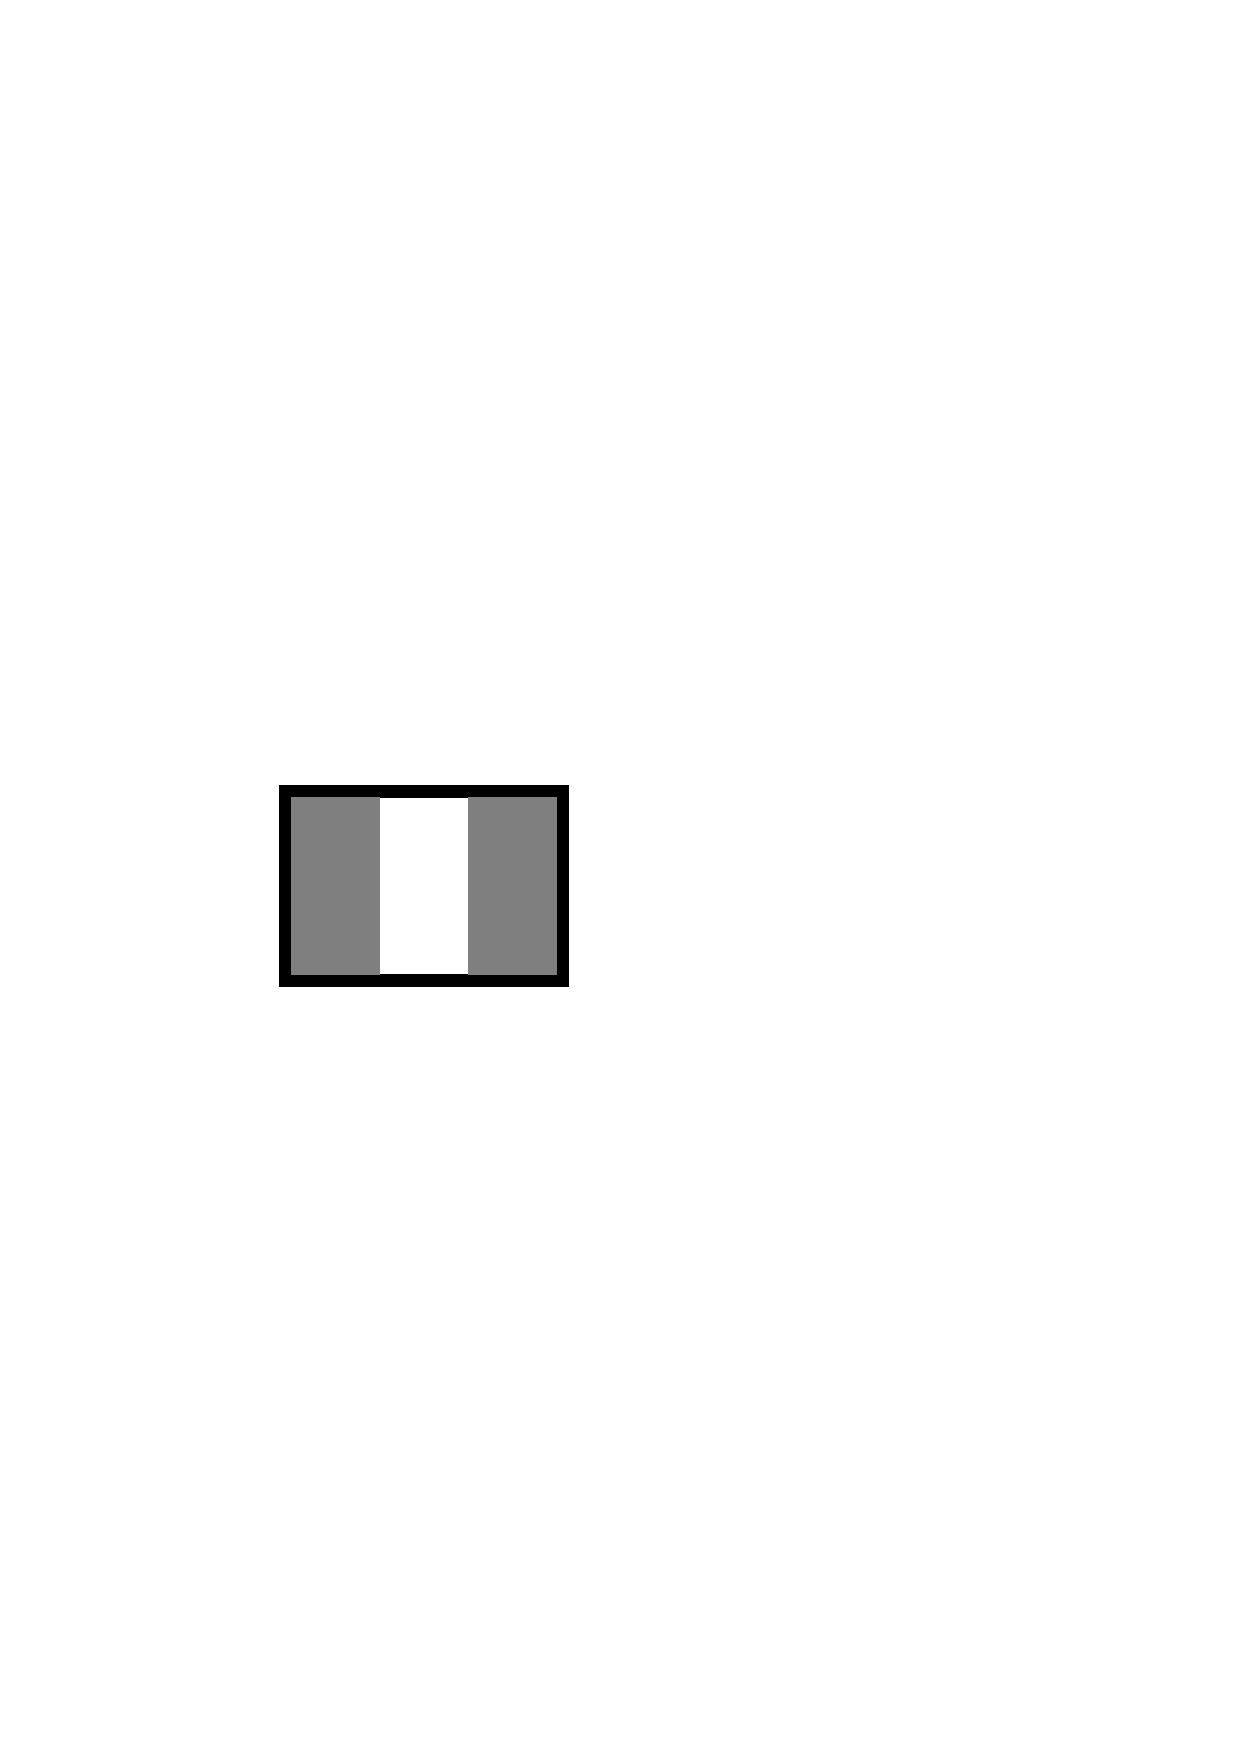
\includegraphics[height=30mm, width=40mm,keepaspectratio]{Logotre}
\caption[Logo di fantasia]{\raggedright Logo di fantasia}
\end{wrapfigure}
Il lettore non si scoraggi: questi sono ritocchi destinati a rifinire la tesi quando la si è sostanzialmente completata. Non ho mai usato \cs{goodpagebreak} in modo orizzontale in questa documentazione; l'ho usato in modo verticale solo due o tre volte.

Infine il comando \cs{captionof} serve per assegnare una didascalia ad un oggetto che avrebbe potuto, ma che non è stato composto all'interno di un ambiente mobile come \amb{figure} o \amb{table}.
Il pacchetto \pack{caption} lo definisce, ma se l'utente di \TOPtesi non lo ha caricato, questo comando non sarebbe disponibile. Invece \TOPtesi lo definisce nel caso che, appunto, non sia disponibile. La sua sintassi è semplice: \cs{captionof}\marg{nome di float}\marg{didascalia}. Tuttavia l'abitudine di inserire dei (piccoli) oggetti con didascalia in ambienti fissi in display all'interno del testo, deriva dal desiderio di imitare il comportamento dei word processor. Io ritengo che non sia una buona pratica, ma forse è solo una questione di gusti personali; esistono altri modi per inserire (piccoli) oggetti più o meno flottanti e dotati della loro didascalia ricorrendo a pacchetti esterni come \pack{wrapfig} che permette di inserire un oggettino flottante con tanto di didascalia sia nel margine, sia nel testo, ma con il testo che lo avvolge; oppure usando il pacchetto \pack{sidecap} e i suoi ambienti (vedi documentazione), che permette di comporre la didascalia a fianco invece che sotto o sopra l'oggetto; il fatto di avere disponibile il lato della figura ed eventualmente il margine della pagina per disporvi la didascalia permette di risparmiare un poco di spazio verticale o di sfruttare meglio lo spazio a fianco di una figura  relativamente stretta.

\section{Comandi per il frontespizio}
\textcolor{red}{Questo paragrafo descrive i comandi per comporre il frontespizio con i moduli di \TOPtesi (vedi la tabella~\ref{tab:tipotesi}). Se si vuole comporre il frontespizio con un altro pacchetto, non si usino questi comandi ma quelli descritti nella documentazione del pacchetto alternativo. Naturalmente si sarà specificata l'opzione  giusta, o \chiave{tipotesi}{custom} o \chiave{tipotesi}{frontespizio}, fra le opzioni della classe.}

{\tolerance=3000\textcolor{red}{I comandi per la composizione del frontespizio \emph{non possono} essere inseriti nel preambolo, cioè  prima di \Bambiente{document}, qualunque sia il programma di compilazione usato, perché nessuno di quei comandi è definito prima che il modulo scelto sia stato eventualmente caricato, il che avviene solo al momento di eseguire il comando \Bambiente{document}.}\par}

È per questo che si consiglia di usare facoltativamente il file di configurazione e/o di inserire  i comandi necessari per il frontespizio, non presenti nel file di configurazione, all'interno degli ambienti destinati alla composizione dei vari frontespizi. In questo modo non si corre il rischio di inserirli nel preambolo. Se poi si usa un pacchetto esterno per comporre il frontespizio, a maggior ragione bisogna specificare i comandi necessari come specificato nella documentazione di quel pacchetto esterno.

I comandi di questa sezione possono essere introdotti in un ordine qualunque, ma è  più chiaro se sono introdotti nell'ordine in cui sono elencati nelle tabelle~\ref{tab:front1}-\ref{tab:front4} riportate dalla pagina~\pageref{tab:front1} alla pagina~\pageref{tab:front4}.

Alcuni comandi sono generali; altri si riferiscono specificatamente alla monografia di laurea, o alla tesi laurea, o alla dissertazione dottorato. In una colonna di queste tabelle vi è indicato la sigla del modulo per il quale quel comando  è valido; se manca questa sigla, il comando vale per tutti i moduli. Le sigle sono `t' per la triennale, `m' per la magistrale, `d' per la dottorale, `S' per la tesi dottorale della ScuDo, `n' per usare il modulo di default, e `s' per la tesina della scuola secondaria.

Per le tesi dottorali della ScuDo si veda più avanti il paragrafo~\ref{sec:frontescudo}.

La differenza è che generalmente la tesi di laurea triennale non ha un relatore; se nella vostra facoltà anche la monografia di laurea ha un relatore comportatevi come per la tesi di laurea cambiandone il nome mediante il comando \cs{NomeElaborato} e cambiando il nome del corso di studi con \cs{NomeCorsoDiStudi}. 

Similmente si cambino le stringhe inserite dai vari comandi facendo ampio uso di quelli esposti nelle tabelle~\ref{tab:front1}--\ref{tab:front4}; in particolare consiglierei di inserirli nel file di configurazione, specialmente se devono rappresentare delle modifiche ``permanenti''. \textcolor{red}{Sono da usare anche per predisporre quelle stringhe in una lingua diversa dall'italiano}.

Per comporre questo testo si è usata la classe \class{toptesi},
e si è supposto di scrivere una monografia; tuttavia alcune
delle stringhe di default non sono adeguate a questo uso, quindi il
preambolo di questo documento contiene le seguenti specificazioni
che illustrano l'impiego di diversi fra i comandi descritti nelle
tabelle citate:
\begin{Verbatim}[fontsize=\footnotesize]
\begin{ThesisTitlePage}
\GetFileInfo{toptesi.cls}% per recuperare versione e data della classe
\let\classvers\fileversion \let\classdate\filedate
\logosede{TITlogoCropped}
\NomeElaborato{Manuale d'uso}
\titolo{Il pacchetto \TOPtesi\\
\textnormal{\normalsize Versione\ \classvers\ del \classdate}}
\TitoloListaCandidati{}
\sottotitolo{Per comporre tesi al Politecnico di Torino
   \\e in molte altre università\\[1ex]
...}
\GetFileInfo{toptesi-it.tex}% per recuperare versione e data di questa
%                             documentazione
\sedutadilaurea{Documentazione: versione \fileversion\ del \filedate}
\retrofrontespizio{Questo testo è libero secondo le condizioni 
...}.
 
\bigskip
 
\noindent Composto con \ifPDFTeX \pdfLaTeX
\else \ifXeTeX\XeLaTeX
\else\ifLuaTeX\LuaLaTeX
\else un programma diverso\fi\fi\fi\ 
il \today \vspace*{5\baselineskip}}
\end{ThesisTitlePage}
\end{Verbatim}

Naturalmente per usare l'ambiente \amb{ThesisTitlePage} ho usato il modulo per le tesi triennali/monografie specificando anche \chiave{tipotesi}{monografia} fra le opzioni della classe. Inoltre ho usato il comando \cs{titolo} che, lo si ricorda, per le monografie non è disponibile con il pacchetto di default \pack{topfront}.

\begin{figure}[p]\centering
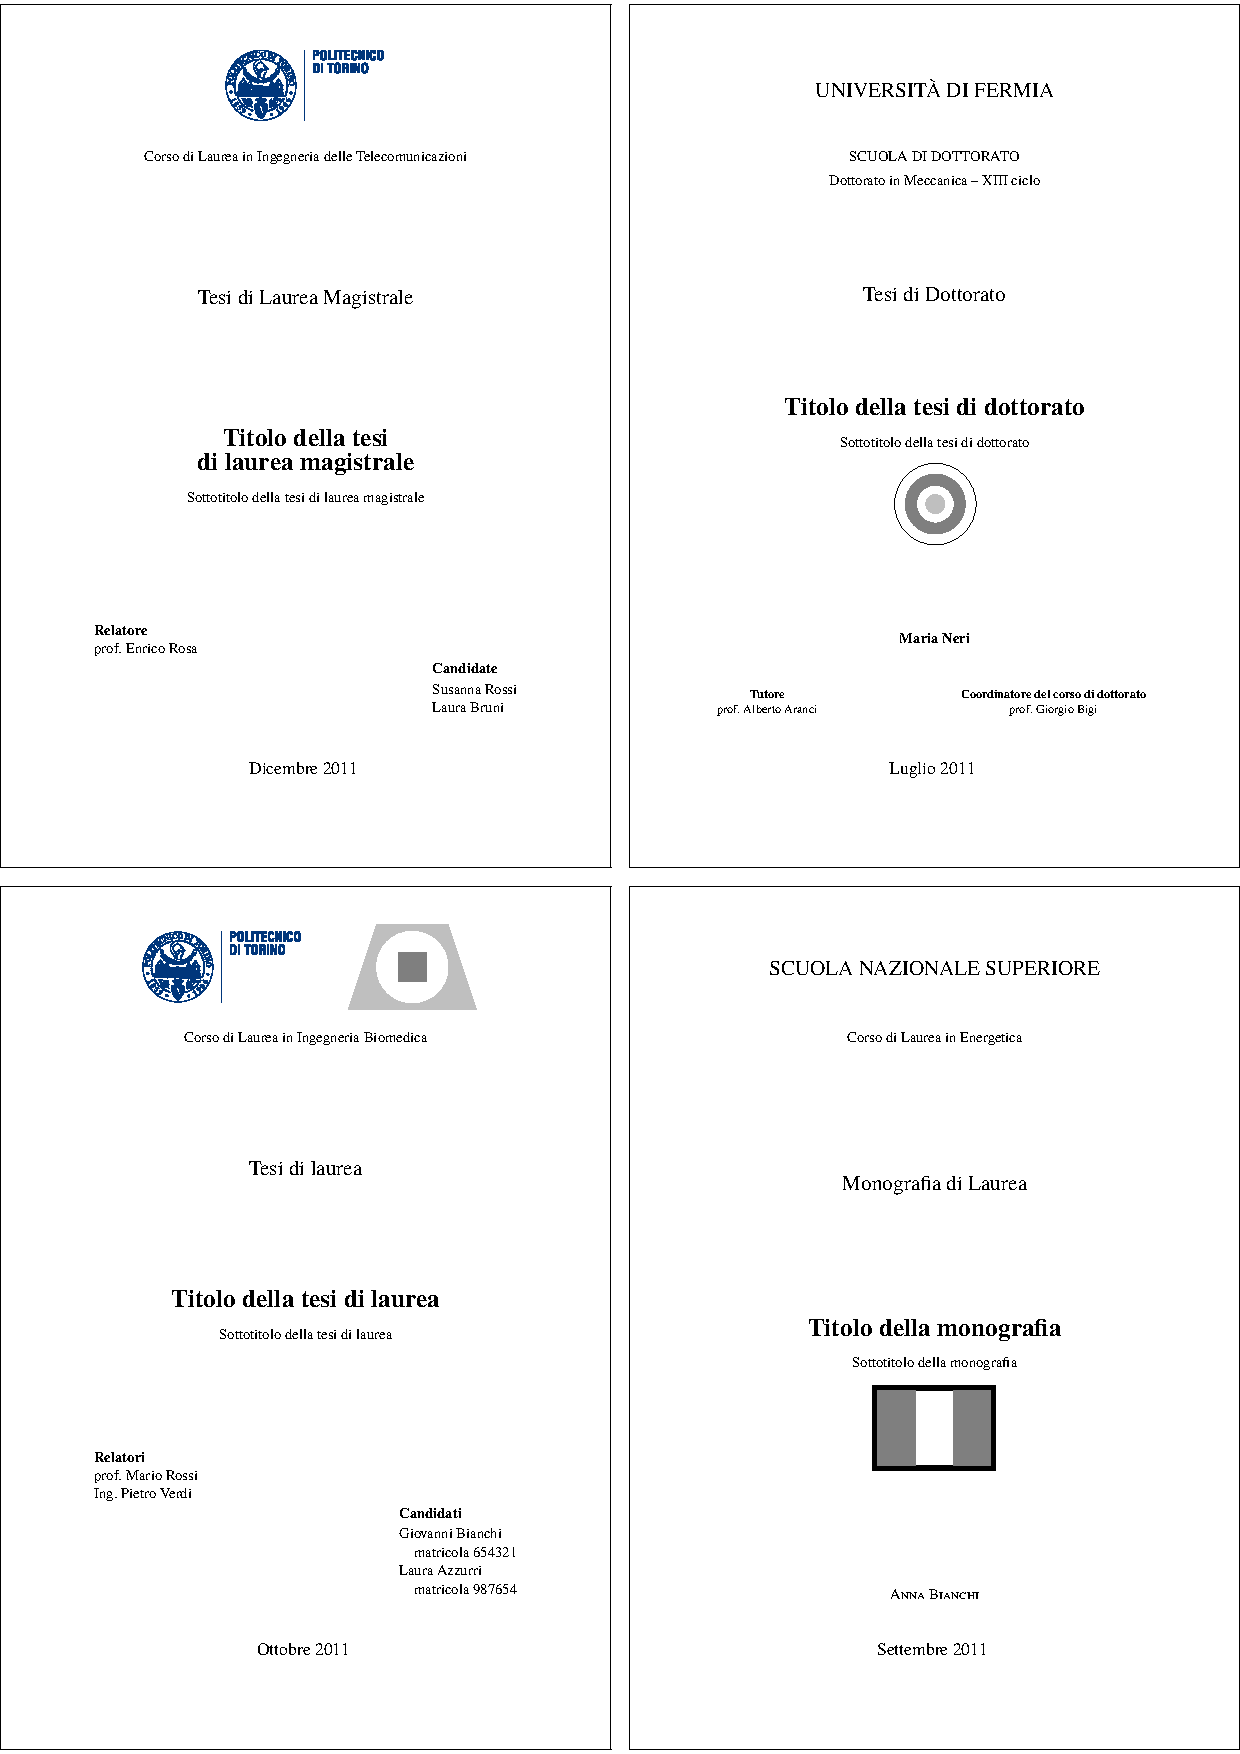
\includegraphics[height=.9\textheight]{FrontespiziAssemblati}
\caption{I quattro frontespizi fondamentali}\label{fig:frontespizi}
\end{figure}

Vale la pena di fare le seguenti osservazioni.
\begin {enumerate}[noitemsep]
\item Il comando \cs{NomeElaborato} può servire per diversi scopi. In questo particolare documento che non è una tesi di laurea triennale, lo si è usato per qualificare il contenuto il nome ``Manuale d'uso''. In altre circostanze può servire per impostare il nome del documento in una lingua straniera; oppure per una laurea triennale che richieda l'indicazione anche di uno o più relatori, è possibile usare il modulo per la laurea magistrale, cambiando il nome dell'elaborato in ``Tesi di laurea triennale'' e cambiando il nome del corso degli studi con \cs{NomeCorsoDiStudi} in ``Corso di laurea triennale''.
%
\item Se per comporre la pagina del titolo si usa un ambiente senza asterisco, il logo viene messo in testa; se si usa la forma asteriscata il logo viene messo nella metà inferiore della pagina del titolo. Se il logo dell'ateneo contiene per disteso il logotipo, cioè il nome per disteso, allora l'uso del comando \cs{ateneo} contenente il nome generico dell'ateneo implica una ridondanza di informazioni che potrebbe anche essere antiestetica; quindi se si usa il comando \cs{ateneo} sarebbe meglio usare un ambiente asteriscato, e viceversa. Ma questa possibilità di scelta per la posizione del logo e la presenza del nome dell'ateneo consente di rispettare le diverse specifiche indicate dalle segreterie didattiche degli atenei; si veda la tabella riassuntiva~\ref{tab:modalitaperfrontespizi} nella pagina~\pageref{tab:modalitaperfrontespizi}.
%
\item Il comando \cs{titolo} non è disponibile per la monografia nel modulo di default \pack{topfront}, mentre negli altri moduli  esso è definito e si può usare tranquillamente anche per la monografia.
%
\item Il comando \cs{titolo} accetta un argomento facoltativo, la versione breve del titolo del frontespizio; serve con  \chiave{stile}{classica} e l'opzione \opt{autoretitolo}, perché  il titolo  breve va  nella testatina delle pagine; se il titolo del frontespizio fosse troppo lungo la testatina verrebbe molto, molto male!
%
\item Se non si danno i comandi \cs{relatore}, \cs{secondorelatore}
e \cs{terzorelatore} non viene scritto nulla nel frontespizio che riguardi questi ruoli; di solito né per la dissertazione di dottorato né per la monografia si hanno le figure dei relatori, ma ``di solito'' non vuol dire né ``sempre'' né ``mai''.
%
\item Si nota l'uso del comando \cs{TitoloListaCandidati} con un argomento vuoto. Questo comando serve per impostare il titolo sopra la lista dei nomi degli autori della tesi; esso accetta come argomento una lista di nomi (da zero a quattro) separati da virgole che rappresentano nell'ordine i nomi maschile singolare, maschile plurale, femminile singolare, femminile plurale, da usare come intestazione della lista degli autori. L'argomento nullo implica l'assenza di ogni titolo e, come in questo documento, esso viene usato con un solo nome da comporre centrato, invece che un una ``scatola'' accostata a destra. Gli argomenti non nulli possono venire usati in vari modi; per una data tesi un solo nome potrebbe essere sufficiente; per una impostazione da usare per diverse tesi si elencano solo il singolare e il plurale in quelle lingue in cui non c'è differenza fra maschile e femminile, come l'inglese, lo spagnolo, ed altre; si usano i quattro nomi per le lingue dove singolare e plurale e maschile e femminile sono distinti, come per l'italiano, il tedesco ed altre. Come si vede, quindi, questo comando è utile non solo in questo particolare documento, ma anche quando si vogliono impostare le parole fisse per tesi da comporre in lingue diverse dall'italiano.
%
\item Solo con l'opzione \chiave{stile}{classica} si può ottenere la separazione fra l'intestazione e il nome del relatore, da una parte, e l'intestazione e i nomi dei correlatori. Se i correlatori, che vanno introdotti come se fossero il secondo e il terzo relatore, fossero più di due, allora si sfrutti il trucco seguente (come già, detto valido solo per l'opzione \chiave{stile}{classica}):
\begin{verbatim}
% Solo con  "stile=classica" e solo per laurea magistrale
\relatore{prof.~Giovanni Bianchi}
\secondorelatore{ing.~Lucio Verdi}
\terzorelatore{\tabular[t]{@{}l}
dott.~Mario Rossi\\[0.5ex]
dott.~Piero Neri
\endtabular}
\end{verbatim}

Apparirà l'indicazione Correlatori prima del nome di Verdi seguita dai nomi dei tre correlatori: Verdi, Rossi e Neri.

D'aḹtra parte si può anche usare, adattandolo alle proprie esigenze, il metodo indicato nella pagina~\pageref{proc:titlepage}, dove la tabella dei relatori e correlatori è composta ``a mano''; per esempio, se si volesse indicare una lista di correlatori senza l'opzione \chiave{stile}{classica}, oppure se si volesse aumentare il numero dei relatori oltre il tre, basta inserire la tabella al posto dell'argomento del secondo o del terzo componente della lista, in questo modo (senza l'opzione \chiave{stile}{classica}):
\begin{verbatim}
\AdvisorName{Relatore}
\relatore{prof.~Giovanni Bianchi}
\secondorelatore{\tabular{@{}l}%
\bfseries Correlatori:\\[0.5ex]
ing.~Lucio Verdi\\[0.5ex]
dott.~Mario Rossi\\[0.5ex]
dott.~Piero Neri
\endtabular}
\end{verbatim}
oppure con quattro relatori (sempre senza l'opzione \chiave{stile}{classica}):
\begin{verbatim}
\relatore{prof.~Giovanni Bianchi}
\secondorelatore{ing.~Lucio Verdi}
\terzorelatore{\tabular{@{}l}
dott.~Mario Rossi\\
dott.~Piero Neri
\endtabular}
\end{verbatim}
Il file d'esempio \file{toptesi-example.tex}, da compilare sia con, sia senza l'opzione \chiave{stile}{classica}, contiene diversi modi di usare queste impostazioni.
%
\item L'indicazione della materia su cui si svolge la tesi di laurea o di dottorato non viene normalmente indicata se non, talvolta, nelle facoltà umanistiche.
%
\item I secondi e terzi candidati non hanno senso né per le tesi di dottorato né per le monografie. Per tutti i candidati il comando per inserirne il nominativo accetta due forme:
\begin{flushleft}\obeylines
\cs{candidato}\marg{Nome Cognome}
oppure
\cs{candidato}\marg{Nome Cognome}\oarg{numero di matricola}
\end{flushleft}
Il \meta{numero di matricola} non è quasi mai necessario, quindi l'argomento facoltativo viene usato solo se si vuole indicare anche il numero di matricola perché richiesto dalle prescrizioni dell'ateneo. Se presente, il \meta{numero di matricola} viene composto preceduto da una etichetta ``matricola'' generata dal comando interno \cs{IDlabel} che è predefinito nel modo seguente:
\begin{verbatim*}
\newcommand*\IDlabel{\\\quad matricola\ }}
\end{verbatim*}
e questa definizione corrisponde a scrivere l'etichetta e il numero  con un rientro nella riga sottostante a quella del nome del candidato. Il comando può venire ridefinito dall'utente nel modo che crede più opportuno sia per scrivere l'informazione sulla stessa riga, sia per sostituire la parola ``matricola'' con un'altra, eventualmente in un'altra lingua. Avere il nome del candidato separato dal suo numero di matricola, permette di gestire quest'ultimo separatamente dal primo, in modo che, per esempio, il numero appaia nell frontespizio, ma non appaia nella testatina di sinistra quando è in vigore l'opzione \opz{autoretitolo} nello \chiave{stile}{classica}.
%
\item Per la triennale/monografia l'informazione della data può essere omessa se non c'è una data per la presentazione.
%
\item \TOPtesi inizialmente veniva distribuito con un certo numero di loghi di università italiane e straniere. La politica di \TeXLive è quella di distribuire solo materiale con licenza libera e incondizionata; i loghi delle varie università certamente non lo sono, quindi i loghi non vengono più distribuiti con \class{toptesi}. Ogni laureando è quindi tenuto a chiedere il logo alla sua università accettandone tutte le limitazioni d'uso che l'università potrebbe imporgli.
\end{enumerate}

Per quanto riguarda i loghi, essi implicano l'uso del pacchetto \pack{graphicx}, che perciò \class{toptesi} già carica di default; specificare nuovamente quel pacchetto non produce nessun danno, perché \LaTeX controlla da solo se lo deve caricare o non lo deve ricaricare. Però, evidentemente, lo si è già detto all'inizio, non è bene caricare una seconda volta i pacchetti che sono già stati caricati

\textcolor{red}{Per i formati dei file grafici da includere, le versioni recenti  di \pdfLaTeX, di \XeLaTeX e di \LuaLaTeX accettano i formati PDF, PNG, JPG, MPS, EPS.  La cosa è  scritta a chiare lettere nella guida \file{grfguide.pdf} (già presente nella propria installazione del sistema \TeX aggiornata e completa), ma è  un fatto che viene dimenticato troppo spesso e che obbliga a cercare aiuto da chi ne sa di più, compagni o professori, ma che anche loro talvolta dimenticano.}

\textcolor{red}{Esistono programmi per passare da un formato all'altro, ma anche disponendo di quei programmi e conoscendo i vantaggi e gli svantaggi di un formato rispetto ad un altro, questa operazione viene dimenticata troppo spesso, perché  troppo spesso ci si dimentica di queste limitazioni sui formati.}

Per questo io preferisco usare sempre e solamente i compilatori
\pdfLaTeX,  \XeLaTeX\ o \LuaLaTeX. L'unico inconveniente è che non posso usare direttamente il pacchetto \pack{PSTricks}; ma finora me la sono cavata molto bene anche senza fruire delle prestazioni di questo bellissimo pacchetto. D'altra parte esistono pacchetti che consentono di usare \pack{PSTricks} anche con \pdfLaTeX e gli altri programmi; l'operazione diventa un po' più complicata ma se ne occupa direttamente il programma di tipocomposizione usato; l'utente deve solo caricare uno di quei pacchetti e seguirne le indicazioni specificate nella documentazione (vedi per esempio il pacchetto \pack{pdftricks} già presente in ogni installazione aggiornata e completa di \TeXLive; documentazione: \texttt{texdoc pdftricks}).

\goodpagebreak

\section{Altri comandi}
La classe \class{toptesi} richiede l'uso di altri comandi; con i suoi moduli specializzati compone i frontespizi con ambienti adatti allo scopo; con il suo modulo di default \pack{topfront} ci sono diversi ambienti e programmi per comporre i vari frontespizi dei diversi tipi di tesi. Diciamo che questo modulo di default andrebbe usato il meno possibile perché è conservato per retrocompatibilità e come fallback quando non si usano correttamente le opzioni relative alla chiave \chiave{tipotesi}

Tuttavia se si è costretti ad usare quei comandi o quegli ambienti, si usi solo l'ambiente \amb{frontespizio} con o senza asterisco integrato nel nome, inserendo i dati relativi al frontespizio all'interno dell'ambiente.
 
Merita sottolineare che il formato richiesto dal Politecnico di Torino va bene nel senso che il logo di quell'ateneo contiene già il suo logotipo\footnote{Il logo del Politecnico di Torino è formato da due parti accostate con un piccolo spazio; nella parte di sinistra compare il marchio dell'ateneo, il solito simbolo tondo, mentre la parte di destra contiene il logotipo, cioè il nome \textsf{POLITECNICO DI TORINO} su due righe scritto con certi font e con un colore particolare; font e colore non possono venire modificati, pena la violazione d'uso del logo.}. Sarebbe quanto mai inestetico se in testa al frontespizio comparisse due volte il nome del Politecnico; quindi non è strano che l'intestazione della tesi contenga formalmente solo il logo. Lo stesso potrebbe essere fatto, per esempio, con i loghi di diverse università, per esempio quello dell'Università di Torino, di Ca' Foscari a Venezia, di Bologna, dell'Università Cattolica, di Padova, oltre al logo del Politecnico di Milano, giusto per citarne alcuni, perché già contengono sia il marchio sia il logotipo. Per alcune università, come quella di Urbino, sono disponibili sia il logo col solo marchio, sia il logo completo di logotipo. Nonostante questo alcune facoltà"/scuole"/dipartimenti richiedono l'uso del logo completo in testa alla pagina e la ripetizione del nome dell'ateneo subito sotto. È un vero peccato che quell'ateneo non abbia concordato un tipo standard di frontespizio a cui tutte le facoltà dovrebbero adeguarsi.

Per le università che hanno un nome proprio, come per esempio \emph{Tor Vergata} per la seconda università di Roma ma, che io sappia, non hanno il logotipo nel loro logo, sarebbe quanto mai inestetico usare il logo sopra, in testa, poi il nome proprio, poi tutto il resto; io non consiglierei mai di usare l'ambiente normale in questi casi, ma userei solo quello asteriscato.

Nella figura~\ref{fig:frontespizi} nella pagina~\pageref{fig:frontespizi} sono riportati quattro esempi di frontespizi relativi ai tipi di tesi seguenti:
\begin{itemize}[noitemsep]
\item tesi di laurea  magistrale (o specialistica, secondo una vecchia terminologia),
\item dissertazione di dottorato
\item tesi di laurea del vecchio ordinamento,
\item monografia di laurea,
\end{itemize}
Con questi modelli lo studente che compila la sua tesi usando \textsf{TOPtesi} può scegliere la versione che fa al caso suo e sa anche che cosa deve configurare per eseguire alcuni cambiamenti.


\clearpage

{\rule{1em}{0pt}}{}}\let\t\ttfamily
\makebox[\textwidth]{\footnotesize%
\begin {tabularx}{\linewidth}{p{.25\textwidth}@{\tabcolsep 5pt}cp{.25\textwidth}X}
\hline
Comando o ambiente\V       & sigla  & Default       &  Scopo              \\[.5ex]
\hline
\cs{figurespagetrue}&&\cs{figurespagefalse}&\V Fa o non fa stampare l'indice delle
									 figure\\
\cs{tablespagetrue}&&\cs{tablespagefalse}&Fa o non fa stampare l'indice delle tabelle\\
\amb{frontespizio}  &n&              & Contiene i dati per il 
                                     frontespizio e l'eventuale
																		 retrofrontespizio e lo compone 
																		 con i loghi nella testatina\\
\amb{frontespizio*} &n&              & Contiene i dati per il
                                     frontespizio e l'eventuale
																		 retrofrontespizio e lo compone
																		 con il loghi nella parte bassa 
																		 della pagina\\
\cs{frontespizio}  &n& nessuno       & Fa stampare il frontespizio ed 
                                     eventualmente il
																		 retrofrontespizio; il logo 
																		 dell'ateneo appare in
																		 testa alla pagina \\
\cs{frontespizio*}&n& nessuno	   &	 Fa stampare il frontespizio ed 
                                     eventualmente il
																		 retrofrontespizio; il logo 
																		 dell'ateneo appare in
																		 basso nella pagina; vedi la 
																		 tabella riassuntiva  
																		 \ref{tab:modalitaperfrontespizi}\\
\amb{ThesisTitlePage}&tmdS&& Compone il frontespizio nei vari modi
                             diversi che si applicano ai diversi tipi
                             di tesi; loghi in testa\\
\amb{ThesisTitlePage}*&tmdS&&Compone il frontespizio nei vari modi 
                             diversi che si applicano ai diversi tipi
                             di tesi; loghi in basso\\
\amb{FrontespizioTesina}&s& &Compone il frontespizio per le scuole
                             secondarie\\
\cs{sommario}      &&nessuno        & Inizia un capitolo non numerato 
                                      che ha per
                                      intestazione la parola SOMMARIO 
                                      (anche in lingua)\\
\cs{ringraziamenti}&&nessuno        & Inizia un capitolo non numerato
                                     che ha per intestazione la 
                                     parola
                                     RINGRAZIAMENTI (anche in lingua)
                                     \\
\cs{indici}        &&nessuno        & Fa stampare l'indice generale, 
                                     e, se sono stati dati i comandi
                                 \texttt{\char92figures\-page\-true}
                               e/o \texttt{\char92tables\-page\-true},
                                    anche gli indici delle figure e/o 
                                    delle tabelle.\\
\cs{paginavuota}  &&nessuno       & Emette nel file di uscita una 
																		pagina totalmente bianca, senza 
																		nemmeno il numero della pagina.\\
\cs{NoteWhiteLine}&&nessuno       & Anche questo comando, richiestomi 
																		a gran voce, serve per mettere 
																		in nota una riga bianca.\\[.5ex]
\hline
\end{tabularx}}
\end{table}}

\clearpage

{\rule{1em}{0pt}}{}}\let\t\ttfamily\let\s\string
\caption[Comandi ulteriori con lo stile classico]{Comandi ulteriori per il frontespizio e per il corpo
della tesi definiti con l'opzione \chiave{stile}{classica}. La sigla `c' indica che il comando è specifico dello stile classico.}\label{tab:front5}
\makebox[\textwidth]{%
\begin {tabularx}{\linewidth}{p{.22\textwidth}cX}
\toprule
Comando\V      & sigla &  Scopo              \\[.5ex]
\midrule
\cs{candidato}\V   && Si usa come di solito ma con l'opzione 
											\texttt{classica} produce la scrittura 
					 					``Laureando'' invece che ``Candidato''.\\
\cs{candidata}    & & Come sopra al femminile. Sia questo comando, 
					 						sia il precedente accettano che l'argomento sia 
					 						scritto nella forma 
					 						\marg{Nome Cognome}\oarg{matricola} in alternativa
					 						a \marg{Nome Cognome}.\\
\cs{tomo}        &c & Esegue i frontespizi successivi di una tesi 
					 						divisa in tomi scrivendovi Tomo primo, Tomo 
					 						secondo, eccetera, a seconda del numero 
					 						progressivo dei volumi in cui è suddivisa la 
                      tesi (massimo quattro). Questo comando viene 
                      usato \emph{al posto} di \cs{frontespizio}\\
\cs{annoaccademico}&c& Il suo argomento può essere un anno solare o
                     due anni separati da una lineetta. Viene scritto 
                     nel frontespizio della tesi o del singolo tomo
                     con la specificazione che si tratta dell'anno 
                     accademico e non della data della presentazione 
                     della tesi.\\
\cs{EnDash}        &c& Produce una lineetta lunga come --, ma 
					 						ribassata in modo che stia bene fra numeri di 
					 						stile antico.\\
\cs{nota}\t\d[...] &c& Serve per comporre una nota senza ricorrere al 
					 						contatore numerico di default. Il simbolo con 
					 						cui viene richiamata di default è l'asterisco, 
					 						ma si può mettere qualunque segno matematico 
					 						senza esplicitare i segni di dollaro, per 
					 						esempio si può scrivere
                     {\cs{nota}\t[\s\dagger]\{Questa nota ...\}}\\
\amb{dedica}	  && È un ambiente con cui si può stampare sul recto 
                    di una pagina una dedica; generalmente questa 
                    pagina viene dopo il frontespizio e l'eventuale 
                    retrofrontespizio.\\
\amb{citazioni}  &&  È un ambiente che consente di scrivere una pagina 
				 						con frasi argute. L'arguzia dipende dall'autore; 
										spesso nei libri, raramente nelle tesi, l'autore 
										cita frasi celebri o che in qualche modo hanno 
										a che fare con il contenuto del testo.\\
\bottomrule
\end{tabularx}}
\end{table}}

\clearpage

{\rule{1em}{0pt}}{}}
\caption{Comandi per il frontespizio delle tesi e della dissertazione di dottorato}\label{tab:front1}
\makebox[\textwidth]{\tolerance=9999\finalhyphendemerits=0\footnotesize
\begin {tabularx}{\linewidth}{Xcp{.13\textwidth}>{\raggedright}p{.18\textwidth}p{.25\textwidth}}
\toprule
Comando        & sigla & Default  &  Scopo               &   Esempio d'uso   \\
\midrule
\cs{ateneo}\Marg{...}&ntmd&stringa vuota
                     		& Definisce il nome generico dell'Ateneo 
												& \cs{ateneo}\Arg{II Università di Roma}\\
\cs{nomeateneo}\Marg{...}&ntmd& nessuno
												& Definisce il nome proprio dell'Ateneo 
												& \cs{nomeateneo}\Arg{Tor Vergata}\\
\cs{facolta}\d\Oarg{...}\Marg{...}&ntmd& nessuno 
							& Definisce il nome della Facoltà 
							opzionalmente con l'indicazione 
							dell'ordinale
								& \cs{facolta}\Oarg{III}\d%
								  \Arg{Scienze}\\
\cs{struttura}\d\Oarg{...}\Marg{...}&ntmd&nessuno& sinonimo del
								 comando \cs{facolta}&\\
\cs{corsodilaurea}\d\Marg{...}&ntm& nessuno
							& Definisce il nome del corso di laurea 
								& \cs{corsodilaurea}\d\Arg{Fisica}\\
\cs{corsodidottorato}\d\Marg{...}&nd& nessuno
							&Definisce il nome del corso di dottorato
								&\cs{corsodidottorato}\d\Arg{Fisica}\\
\cs{monografia}\Marg{...}&n&nessuno
							& Definisce il titolo della monografia e 
							  imposta lo stile del frontespizio
								& \cs{monografia}\d\Arg{Il~teorema di 
								Eulero}\\
\cs{titolo}\Oarg{...}\Marg{...}&tmd&nessuno
							& Definisce il titolo  della tesi o della 
							  dissertazione
								& \cs{titolo}\t\d[La~pressione]%
								  \d\Arg{La~pressione di Giove}\\
\cs{sottotitolo}\Marg{...}&ntmd&nessuno
                            & Definisce il sottotitolo della tesi o 
                              della dissertazione
                            & \cs{sottotitolo}\Arg{Metodo Barometrico} \\
\cs{Materia}\Marg{...}&nmd&nessuno
							& Definisce la materia su cui verte 
							  la tesi 
								& \cs{Materia}\Arg{Remote Sensing}\\
\cs{materia}\Marg{...}&nmd&nessuno
							& Sinonimo del comando \cs{Materia} 
								& \cs{materia}\d\Arg{Letteratura 
								  ostrogota}  \\
\midrule
\cambiacorpo{9}
\cs{retrofrontespizio}\d\Marg{...}
				&tmd& nessuno	& \multicolumn2{p{.5\textwidth}}{Se 
								  specificato, serve solitamente per 
								  scrivere nel verso della pagina del 
								  titolo alcune dichiarazioni 
								  di carattere legale; accetta un 
								  argomento composto anche da diversi 
								  capoversi}\\
\bottomrule
\end{tabularx}}
\end{table}

\clearpage

\begin{table}[p]
\def\V{\rule{0pt}{2.5ex}}
\let\s\string \let\t\ttfamily
\def\d{\discretionary{\%}{\rule{1em}{0pt}}{}}
\caption[Comandi per i frontespizi delle tesi universitarie]{Comandi per i frontespizi delle tesi universitarie. L'indicazione della sigla indica che il comando, oltre che certamente presente anche nei moduli specializzati nei diversi tipi di tesi, sono tutti definiti anche nel modulo generico \file{topfront}.}\label{tab:front2}
\makebox[\textwidth]{\small
\begin {tabularx}{\linewidth}{p{.3\textwidth}c>{\raggedright}p{0.1\textwidth}>{\raggedright}Xp{.25\textwidth}}
\toprule
Comando         &sigla& Default  &  Scopo               &   Esempio d'uso   \\
\midrule
\cs{relatore}\Marg{...}\V
				&tmd& nessuno	& Definisce il nome del relatore
								& \cs{relatore}\d
								  \Arg{prof.\s~Albert Einstein} \\
\cs{secondorelatore}\Marg{...}
				&tmd& nessuno	& Se c'è, definisce il nome del 
								secondo relatore
								& \cs{secondorelatore}\d\Arg{dott. %
								  \s~Grazia Deledda}\\
\cs{terzorelatore}\Marg{...}
				&tmd& nessuno	& Se c' è, definisce il nome del
								terzo relatore
								& \cs{terzorelatore}\d
								  \Arg{ing.\s~Thomas A.\s~Edison}\\
\cs{direttore}\Marg{...}
				&d& nessuno	& Definisce il nome del direttore del 
							  ciclo di dottorato
								& \cs{direttore}\d
								  \Arg{prof.\s~Albert Enstein}\\
\cs{coordinatore}\Marg{...}
				&d& nessuno	& Definisce il nome del coordinatore del 
							  ciclo di dottorato
								& \cs{coordinatore}\d
								  \Arg{prof.\s~Albert Einstein}\\
\footnotesize\cs{QualificaDirettore}\Marg{...}
				&d& Direttore o Coordinatore
							& Definisce il titolo da inserire prima 
							  del nome del direttore della scuola di 
							  dottorato
							& \cs{QualificaDirettore}
							  \Arg{PhD~Director}\\
\cs{tutore}\Marg{...}
				&d& nessuno	& Definisce il nome del tutore
								& \cs{tutore}\d
								  \Arg{prof.\s~Karl Von Braun}     \\
\cs{tutoreaziendale}\Marg{...} 
				&tmd& nessuno	& Definisce la qualifica del tutore 
							  aziendale 
								& \cs{tutoreaziendale}\d
								  \Arg{Supervisore}\\
\bottomrule
\end{tabularx}%
}
\end{table}

\clearpage

%\addtocounter{table}{-1}
\begin{table}[p]
\def\V{\rule{0pt}{2.5ex}}
\def\d{\discretionary{\%}{\rule{1em}{0pt}}{}}\let\t\ttfamily
\caption[Comandi per i frontespizi delle tesi universitarie]{Comandi per i frontespizi delle tesi universitarie. L'indicazione della sigla indica che il comando, oltre che  certamente presente anche nei moduli specializzati nei diversi tipi di tesi, sono tutti definiti anche  nel modulo generico \file{topfront}.}\label{tab:front3}
\makebox[\textwidth]{\tabcolsep=3pt\small%
\begin {tabular}{p{.3\textwidth}c>{\raggedright}p{.175\textwidth}p{.26\textwidth}p{.275\textwidth}@{}}
\toprule
Comando        &sigla& Default  &  Scopo               &   Esempio d'uso   \\
\midrule
\cs{candidato}\Marg{...}
				&tmd& nessuno	& Definisce il nome del candidato
								& \cs{candidato}\Arg{Galileo 
                                 Galilei}\\
\cs{candidata}\Marg{...}
				&tmd& nessuno	& Definisce il nome della candidata
								& \cs{candidata}\Arg{Maria Curie}\\
\cs{secondocandidato}\Marg{...}
				&tmd& nessuno	& Se c'è, definisce il nome 
							  del secondo candidato
								& \cs{secondocandidato}\d 
								  \Arg{Evangelista Torricelli}\\
\cs{secondacandidata}\Marg{...}
				&tmd& nessuno	& Se c'è, definisce il nome
							  della seconda candidata
								& \cs{secondacandidata}\d
								  \Arg{Rita Levi Montalcini}\\
\cs{terzocandidato}\Marg{...}
				&tmd& nessuno	& Se c'è, definisce il nome del terzo
								  candidato
									& \cs{terzocandidato}\t\d 
									\Arg{Alessandro~Volta}\\
\cs{terzacandidata}\Marg{...}
				&tmd& nessuno	& Se c'è, definisce il nome della 
								  terza candidata
									& \cs{terzacandidata}\t\d 
									  \Arg{Eleonora~Duse}\\\cs{sedutadilaurea}\Marg{...}
				&tm& data corrente 
								& Definisce il mese e l'anno (volendo
								  il giorno) della seduta di laurea
								& \cs{sedutadilaurea}\t\d 
								  \Arg{Dicembre~2025}\\
\cs{esamedidottorato}\Marg{...}
				&d& data corrente
								& Definisce il mese e l'anno (volendo 
								  il giorno) della seduta di 
								  discussione
									& \cs{esamedidottorato}\t\d 
									  \Arg{Febbraio~2013}\\
\small\cs{scuoladidottorato}\d\Marg{...}
				&d& SCUOLA DI DOTTORATO
								& Definisce il nome ufficiale della 
								  scuola di dottorato
									& \cs{scuoladidottorato}\t\d 
									  \Arg{ScuDo}\\
\cs{ciclodidottorato}\Marg{...}
				&d& nessuno	& Definisce il numero ordinale del 
								  ciclo di dottorato
									& \cs{ciclodidottorato}\t\d 
									  \Arg{XV~ciclo}      \\
\cs{logosede}\Oarg{...}\Marg{...}
				&tmd& nessuno	& \raggedright Inserisce nel 
								  frontespizio il logo dell'ateneo, 
								  specificandone opzionalmente 
								  l'altezza (default: 3\,cm)
									& \cs{logosede}\t\d[2cm]%
									\Arg{logouno,\d logodue}\\
\cs{setlogodistance}\d\Marg{...}
				&tmd& 3\,em		& Imposta la distanza fra i loghi
									& \cs{setlogodistance}\t\d 
									  \Arg{25mm}\\
\bottomrule
\end{tabular}}
\end{table}}

\clearpage

{\rule{1em}{0pt}}{}}
\def\serve{definisce una stringa equivalente a }
 \caption[Comandi per modificare le parole fisse]{Comandi per modificare le parole scritte o per cambiare le parole italiane di default con altre parole diverse o in un'altra lingua}\label{tab:front4}
\makebox[\textwidth]{\cambiacorpo{10}%
\begin{tabular}{@{}p{.35\textwidth}p{.63\textwidth}@{}}
\toprule
\cs{FacoltaDi}\t\{...\}	& definisce una stringa con il nome generico 
						  della struttura didattica, per esempio 
						  ``Scuola di~'', prima del nome della 
						  struttura; di default è impostata una 
						  stringa nulla, cosicché non viene scritto 
						  nulla nel frontespizio in merito alla 
						  struttura didattica competente\\
\cs{StrutturaDidattica}\t\{...\}	 
						& sinonimo del comando  \cs{FacoltaDi}\\
\cs{DottoratoIn}\t\{...\}        
						& \serve ``Dottorato in'' prima del nome 
						  del dottorato\\
\cs{CorsoDiLaureaIn}\t\{...\}    
						& \serve ``Corso di Laurea in'' prima del 
						nome del corso di laurea\\
\cs{TesiDiLaurea}\t\{...\}       
						& \serve ``Tesi di Laurea''\\
\cs{NomeMonografia}\t\{...\}     
						& \serve ``Monografia di Laurea''\\
\cs{NomeDissertazione}\t\{...\}  
						& \footnotesize\serve ``Dissertazione di 
						  Dottorato''\\
\cs{NomeElaborato}\t\{...\}
						& Imposta il nome dell'elaborato valido anche per 
						il modulo per le tesi triennali\\
\cs{InName}\t\{...\}             
						& \serve ``in''; in tedesco potrebbe essere 
						``auf'', in francese ``en'', ecc.\\
\cs{CandidateName}\t\{...\}      
						& \serve ``Candidato''; per questo e i due 
						comandi successivi il programma riesce a 
						scegliere la stringa giusta adattata in 
						numero genere; nel cambiare queste stringhe 
						il compositore ha una sola possibilità e deve 
						scegliere direttamente il genere e il numero.
						\\
\cs{TitoloListaCandidati}\t\{...\}
						& \serve per definire una lista di nomi separati 
						da virgole per impostare le parole equivalenti a 
						``Candidato'' nel genere e numero specifico; da 
						usare sia per impostare una lista vuota, sia per 
						impostare la lista in lingue diverse dall'italiano\\
\cs{AdvisorName}\t\{...\}        
						& \serve ``Relatore''\\
\cs{CoAdvisorName}\t\{...\}      
						& \serve ``Correlatore''; questo comando si 
						può usare sempre, ma il suo contenuto viene 
						effettivamente usato  solo se si specifica 
						l'opzione \texttt{classica}; se in italiano 
						non piace ``Correlatore'' ma si preferisce 
						``Corelatore'' o ``Co-relatore'', sempre con 
						l'opzione \texttt{classica}, si può 
						correggere la versione di default.\\
\cs{TutorName}\t\{...\} & \serve ``Tutore''\\
\cs{NomeTutoreAziendale}\t\{...\}
						& \serve ``Supervisore aziendale''; usando un 
						argomento che contenga anche indicazioni di 
						``a capo'', nella seconda riga si può 
						scrivere il nome dell'azienda.\\
\cs{CycleName}\t\{...\} & \serve ``ciclo''; serve essenzialmente 
						per indicare il ciclo di dottorato\\
\cs{NomePrimoTomo}\t\{...\}      
						& \serve ``Tomo primo''\\
\cs{NomeSecondoTomo}\t\{...\}    
						& \serve ``Tomo secondo''\\
\cs{NomeTerzoTomo}\t\{...\}      
						& \serve ``Tomo terzo''\\
\cs{NomeQuartoTomo}\t\{...\}     
						& \serve ``Tomo quarto''; tutte e quattro 
						queste stringhe dipendono dalla lingua 
						usata e dall'ordine che si vuole o si deve 
						dare alle due parole.\\
\bottomrule
\end{tabular}}
\end{table}
}


%>!
\clearpage

\begin{otherlanguage}{english}

\section{ ScuDo title page commands}\label{sec:frontescudo}

The \file{toptesi-scudo.sty} module contains all the definitions necessary to typeset the thesis title page. Some of the commands just set the ``fixed'' parts of the title page; other are used to enter the variable parts, that is pieces of information such as the thesis author, title, defence date, and the like. All parts, fixed or variable have specific default values. Here we describe just the user commands divided in two sets, the most important and compulsory variant data, and the customisation of ``fixed'' data.

\subsection{Variant data}
All commands to insert variant data accept one mandatory argument.
\begin{description}[noitemsep]
\def\Item[#1]{\item[\normalfont\cs{#1}]}
%
\Item[Cyclenumber] Defines a string that represents the ordinal number of the cycle program. This ordinal may be written in a variety of ways, from ``29\ap{th}'', to ``29.th''; from ``Twenty\-ninth'', to ``XXIX''. If the ordinal number string is not specified, its label ``cycle'' is omitted.
%
\Item[ProgramName] The argument is the name of the discipline the thesis is about, it may be composed with several words. Default empty.
%
\Item[author] The argument is the thesis author's name(s) and surname(s) without any separator except the necessary inter word spaces. Default empty.
%
\Item[title] The argument is the thesis title; keep it short. Default empty.
%
\Item[subtitle] The subtitle is a second string that describes and complements the thesis title in order to maintain short the thesis title. Default empty.
%
\Item[SupervisorList] Defines a list of supervisors and co-supervisors with their roles; the names are separated with a 
\verb|\\| command; an example would be:
\begin{verbatim}
    \SupervisorList{%
        prof. John Smith, Supervisor\\
        prof. Jack Brown, Co-supervisor
    }
\end{verbatim}
Default empty.
%
\Item[ExaminerList] By default the defined string is empty. When the title page is being printed, if this list is still empty, no examiner list is printed and, of course, also its label is omitted. Otherwise the list is printed together with its label. Example:
\begin{verbatim}
    \ExaminerList{%
        prof. John Smith, Referee, University of Berlin\\
        prof. Jack Brown, Referee, University of Vienna\\
        prof. Jane White, University of Eton\\
        prof. Jay  Black, University of Washington\\
        ...
    }
\end{verbatim}
%
\Item[ExaminationDate] Defines the full date of the examination: ``location, day of month year'' in European style; ``location, month, day year'' in USA style . Default empty. Example in European style:
\begin{verbatim}
\ExaminationDate{Turin, 29 of February 2345}
\end{verbatim}
%
\end{description}


\subsection{Fixed data}

All the fixed data have a default value consisting in a character-string.
\begin{description}[noitemsep]
\def\Item[#1]{\item[\normalfont\cs{#1}]}
%
\Item[PhDschoolLogo] Specifies the name of the file that contains the School Logo. Default none; the file extension may be omitted, but the real extension should be one of \file{.pdf}, \file{.eps}, \file{.png}, \file{.jpg}. Actually this command accepts a list of comma separated names of Doctoral School logos, even if they are under control of the ScuDo school. We refer to the partnerships that ScuDo has with Università di Torino and with Istituto Nazionale di Ricerca Metrologica (INRiM). When a doctoral thesis is supported by INRiM or is a joint Doctoral Thesis with the University of Turin, their logos are supposed to be set in the title page; such logos, as well as the ScuDo one are available form the Students Office or downloaded from a specific restricted Web site.

Please, take notice that ScuDo has available four different logos (to be asked for at the Student Office); the four variants of the school logo are: $(a)$ \texttt{Logo-ScuDo.pdf} (a black and white logo without any decoration at its sides; may be it is an old school logo); $(b)$  \texttt{Logo-ScuDo-RGB.pdf} (an inverted color logo with decoration at its right, with white and yellow inscriptions over a blue background); $(c)$ \texttt{Logo-ScuDo-BN-RGB\discretionary{}{.}{.}pdf} (a black and white logo with decorations at its right; a new logo, the one you probably should use); $(d)$ \texttt{Logo-ScuDo-blu-RGB\discretionary{}{.}{.}pdf} (a blue on white logo with decorations at its right; the blue tint is the official blue required by most internal documents of Politecnico di Torino).  This bundle does not contain any official logo, because these trademarked images are property of the respective entities, and cannot be freely distributed under the permissive LPPL licence common to most \TeX system software.

%\iffalse
%  See figure~\ref{fig:scudologos}.
%  
%  \begin{figure}[!htb]\centering
%  
%  \makebox[0pt][l]{\raisebox{14mm}[0pt][0pt]{$(a)$}}%
%  \makebox[\textwidth]{\includegraphics[height=30mm]{Logo-ScuDo.pdf}}
%  
%  \bigskip
%  
%  
%  \makebox[0pt][l]{\raisebox{14mm}[0pt][0pt]{$(b)$}}%
%  \makebox[\textwidth]{\includegraphics[height=30mm]{Logo-ScuDo-RGB.pdf}}
%  
%  \bigskip
%  
%  \makebox[0pt][l]{\raisebox{14mm}[0pt][0pt]{$(c)$}}%
%  \makebox[\textwidth]{\includegraphics[height=30mm]%
%          {Logo-ScuDo-BN-RGB.pdf}}\bigskip
%  
%  \makebox[0pt][l]{\raisebox{14mm}[0pt][0pt]{$(d)$}}%
%  \makebox[\textwidth]{\includegraphics[height=30mm]%
%          {Logo-ScuDo-blu-RGB.pdf}}
%  
%  \bigskip
%  
%  \caption{The four logos available for the ScuDo doctoral school}
%  \label{fig:scudologos}
%  \end{figure}
%\fi

The last three logos were provided by the specific office of Politecnico di Torino in EPS format and CMYK color profile; very large files due to the verbosity of the PostScript commands and to the fact that such files contained  both the EPS code and the compressed bitmapped image. By using the \prog{Inkscape} program as described in the English documentation \file{toptesi.pdf}, these PDF/A incompatible images were converted to pure EPS code and RGB profile; they were further processed to transform them in PDF/A compliant format. Hopefully these transformations should be much handier than the original images. In any case, remember that these four logos are not part of this bundle, but you have to ask the school Student Office in order to receive the logo file directly o the authorisation to download it from a restricted Web site.
%
\Item[Ndissertation] Specifies the name of the dissertation. Default ``Doctoral Disseration''.
%
\Item[Ndoctoralprogram] Specifies the name of the doctoral program. Default ``Doctoral program in\cs{xspace}'' where the \cs{xspace} macro inserts a smart space if it is needed.
%
\Item[Nsupervisor] Specifies through two separate arguments the singular and the plural name to label the supervisor list. Default ``Supervisor'' and ``Supervisors''.
%
\Item[SupervisorNumber] Specifies the number of supervisors. Default ``0'' (zero); actually by specifying an empty argument, is the same as specifying ``0''; with this number set to zero or to empty, no label is set above the list of supervisors; the real turning point is the specification ``1'' when the singular label is used; any other value greater then ``1'',  is treated as ``many'' and implies the plural label.
%
\Item[Nexaminationcommittee] Specifies the label to print above the list of examiners. Default ``Doctoral Examination Committee''.
%
\Item[Nlocation] Specifies the full official name of the institution where the doctoral examination is held. Default ``Politecnico di Torino''. This suffices for the ScuDo dissertation, but for other doctoral schools it might be necessary to specify also  the city, the province"/state and sometimes the nation.
%
\Item[Property] Specifies the claim for the intellectual property of the Ph.D.\ dissertation contents. Default ``This thesis is licensed under a Creative Commons License, Attribution - Noncommercial- NoDerivative Works - 4.0 International: see \begin{center}\url{www.creativecommons.org}.\end{center}
The text may be reproduced for non-commercial purposes, provided that credit is given to the original author.''
%
\Item[Disclaimer] Specifies the text of the disclaimer statement. Default ``\cs{noindent} I hereby declare that the contents and organisation of this dissertation constitute my own original work and does not compromise in any way the rights of third parties, including those relating to the security of personal data.''
%
\Item[Signature] Specifies the signature field with a dotted line to hand-sign the statement, the signer's name, the place of signature and the signature date. The signer's name defaults to the author's name, and the date defaults to the examination date. This latter default perhaps should be modified. In any case the command definition provides a default layout as such:
\begin{verbatim}
\begin{flushright}
\parbox{0.5\textwidth}{%
\centering
\dotfill\\
\@author\\
Turin, \@examinationdate
}%
\end{flushright}
\end{verbatim}
An actual user might redefine the \cs{Signature} macro so as to provide anther layout, for example:
\begin{flushleft}\obeylines
\cs{renewcommand}\Marg{\char92Signature}\Marg{\%
\quad\Bambiente{flushright}
\qquad\cs{parbox}\Marg{0.5\cs{textwidth}}\Marg{\%
\qquad\quad\cs{dotfill}\string\\
\qquad\quad\meta{name surname}\string\\
\qquad\quad\meta{city}, \meta{date}}
\quad\Eambiente{flushright}
}
\end{flushleft}
%
\end{description}

\subsection{The title page}
Most if not all fixed data commands may be written down once and for all in the configuration file \file{.cfg}.

Variant data, probably, find their best place within the title page environment. In any case such environment is the first one that produces text in the output file. It has the following structure.
\begin{flushleft}\obeylines
\Bambiente{\normalfont\amb{ThesisTitlePage}}
\quad\meta{fixed data}
\quad\meta{variant data}
\Eambiente{\normalfont\amb{ThesisTitlePage}}
\end{flushleft}

An example title page is shown in figure~\ref{fig:frontescudo} on page~\pageref{fig:frontescudo}.

\end{otherlanguage}

\backmatter

\chapter*{Conclusioni}
\addcontentsline{toc}{chapter}{Conclusioni}

Il pacchetto \textsf{TOPtesi} fa quasi tutto quello che è necessario per comporre uno qualunque di quegli scritti che vengono chiamati \emph{monografia di laurea}, \emph{elaborato finale di laurea},  \emph{tesi di laurea}, \emph{tesi di laurea triennale}, \emph{tesi di laurea specialistica}, \emph{tesi di laurea magistrale}, \emph{dissertazione di dottorato} (con l'aggiunta anche della \emph{tesina} per l'esame di stato delle scuole secondarie superiori).

Non fa tutto, ci mancherebbe altro, visto che nessuno è in
grado di prevedere tutte le necessità altrui.

Da un lato alcuni utenti devono adattarsi a quello che è disponibile, magari dandosi da fare per creare qualche cosa di nuovo e utile per se stessi e forse anche per gli altri. Qualcun altro deve sapersi immedesimare nelle necessità altrui e magari deve darsi da fare per creare qualcosa di nuovo e utile agli altri e forse anche a se stesso.

Il modo di localizzare le stringhe fisse dovrebbe risultare semplificato rispetto alle versioni fino alla 5.x.xx di \TOPtesi, grazie ai moduli separati per i vari tipi di tesi; ogni frontespizio richiede un numero ristretto di stringhe fisse rispetto al caso generale; quindi il lavoro di localizzazione riguarda, a seconda delle tesi, fino a una dozzina di casi. 

\textcolor{red}{%
\english For the ScuDo doctoral school some packages are preloaded in addition to those already loaded by the \TOPtesi bundle. The title page for this doctoral school is obtained with its own commands and environment. The appearance of this title page was shown in figure~\ref{fig:frontescudo} on page~\pageref{fig:frontescudo}, and the general instructions for this title page are given in section~\ref{sec:frontescudo}. Doctoral students benefit from examining the source file \file{toptesi-scudo-example.tex} (already part of this bundle) where many details are added for using this particular variant.}

Il pacchetto \textsf{TOPtesi} carica di default sia \texttt{babel} o \texttt{polyglossia} sia \texttt{graphicx}; certo potrebbe caricare di default anche \texttt{amsmath} e i suoi compagni, ma non tutti hanno bisogno di scrivere e comporre matematica avanzata e se non vengono usati essi comportano uno risparmio di memoria e un sia pur piccolo miglioramento nell'esecuzione. Ritengo quindi che sia meglio che ognuno si carichi i pacchetti che intende davvero usare.

\goodpagebreak

Consiglierei l'uso  di \XeLaTeX solo per quelle tesi, specialmente di carattere umanistico, che hanno bisogno di maneggiare agevolmente font di diversi tipi per scrivere con alfabeti o sillabari o sistemi di ideogrammi per i quali \pdfLaTeX\ è, sì, attrezzato, ma rende molto più faticosa l'intera operazione. 

Più interessante è il programma di composizione \LuaLaTeX, che incorpora una buona parte del linguaggio di scripting Lua; questo a sua volta permette di compiere diverse azioni esternamente al programma di tipocomposizione (mi risulta che sia usato per impostazione predefinita per comporre la musica gregoriana con il pacchetto \pack{GregorioTeX}); in certi casi esso si può considerare una estensione molto utile del programma \pdfLaTeX. Benché questo programma possa usare la microtipografia come \pdfLaTeX\ e i font OpenType come \XeLaTeX, vale la pena di usarlo al posto di quest'ultimo, se non altro perché ne è un superset che riesce a fare altre cose oltre quelle che \XeLaTeX\ è in grado di fare; in particolare può produrre file archiviabili secondo le norme ISO senza bisogno di nessun tipo di post"processing.

So per certo che le tesi di filologia classica possono essere composte molto bene con \pdfLaTeX\ e \textsf{TOPtesi}; se bisogna usare una buona dose di lingua greca classica  è conveniente caricare il pacchetto \pack{teubner}\footnote{A tutt'oggi (\the\year) il pacchetto \pack{teubner} funziona correttamente solo con \pdfLaTeX.}; gli intenditori sanno perfettamente che i font greci della casa editrice Teubner di Lipsia sono fra i più gradevoli che esistano; il pacchetto \texttt{teubner} fa uso di un'ottima imitazione di quei font e mette a disposizione una miriade di comandi per comporre quei segni ``strani'' che i filologi usano per scrivere le loro opere.

Per le edizioni critiche esistono i pacchetti \texttt{eledmac} e \pack{reledmac}; io non li ho mai usati, ma sembra che siano di grande aiuto per gli umanisti.

Per gli scienziati e i tecnologi esistono troppi pacchetti specializzati e sarebbe impossibile, e forse inutile, elencarli tutti o anche elencare solo i più importanti.

Non resta che augurare:
\begin {center}\cambiacorpo{16}\bfseries
Buona composizione con \pdfLaTeX\ o \LuaLaTeX\ o~\XeLaTeX!
\end{center}

\begin{center}
\color{red}\cambiacorpo{16}\bfseries
Happy \TeX{ing} with \pdfLaTeX, or \LuaLaTeX, or~\XeLaTeX!
\end{center}

\english
\appendix
\chapter{The \LaTeX\ Project Public License}\label{ch:LPPL}
\begin{otherlanguage}{english}
%=-=-=-=-=-=-=-=-=-=-=-=-=-=-=-=-
\begin{quote}
LPPL Version 1.3,  2003-12-01

Copyright 1999 2002-03 \LaTeX3 Project

    Everyone is allowed to distribute verbatim copies of this
    license document, but modification of it is not allowed.
\end{quote}

\section{Preamble}
%========

The \LaTeX\ Project Public License (LPPL) is the primary license under
which the the \LaTeX\ kernel and the base \LaTeX\ packages are
distributed.

You may use this license for any work of which you hold the copyright
and which you wish to distribute.  This license may be particularly
suitable if your work is \TeX-related (such as a \LaTeX\ package), but
you may use it with small modifications even if your work is unrelated
to \TeX.

The section `Whether and How to Distribute Works under This License',
below, gives instructions, examples, and recommendations for authors
who are considering distributing their works under this license.

This license gives conditions under which a work may be distributed
and modified, as well as conditions under which modified versions of
that work may be distributed.

We, the \LaTeX3 Project, believe that the conditions below give you the
freedom to make and distribute modified versions of your work that
conform with whatever technical specifications you wish while
maintaining the availability, integrity, and reliability of that work.
If you do not see how to achieve your goal while meeting these
conditions, then read the document `cfgguide.tex' and `modguide.tex' in
the base \LaTeX\ distribution for suggestions.


\section{Definitions}
%===========

In this license document the following terms are used:
\begin {description}\def\Item[#1]{\item[\textit{#1}]}
\Item[Work]
    Any work being distributed under this License.

\Item[Derived Work]
    Any work that under any applicable law is derived from the Work.

\Item[Modification]
    Any procedure that produces a Derived Work under any applicable
    law -- for example, the production of a file containing an
    original file associated with the Work or a significant portion of
    such a file, either verbatim or with modifications and/or
    translated into another language.

\Item[Modify]
    To apply any procedure that produces a Derived Work under any
    applicable law.

\Item[Distribution]
    Making copies of the Work available from one person to another, in
    whole or in part.  Distribution includes (but is not limited to)
    making any electronic components of the Work accessible by
    file transfer protocols such as FTP or HTTP or by shared file
    systems such as Sun's Network File System (NFS).

\Item[Compiled Work]
    A version of the Work that has been processed into a form where it
    is directly usable on a computer system.  This processing may
    include using installation facilities provided by the Work,
    transformations of the Work, copying of components of the Work, or
    other activities.  Note that modification of any installation
    facilities provided by the Work constitutes modification of the Work.

\Item[Current Maintainer]
    A person or persons nominated as such within the Work.  If there is
    no such explicit nomination then it is the `Copyright Holder' under
    any applicable law.

\Item[Base Interpreter]
    A program or process that is normally needed for running or
    interpreting a part or the whole of the Work.
    A Base Interpreter may depend on external components but these
    are not considered part of the Base Interpreter provided that each
    external component clearly identifies itself whenever it is used
    interactively.  Unless explicitly specified when applying the
    license to the Work, the only applicable Base Interpreter is a
    ``\LaTeX-Format''.
\end{description}


\section{Conditions on Distribution and Modification}
%===========================================
\begin {enumerate}
\item  Activities other than distribution and/or modification of the
Work are not covered by this license; they are outside its scope.  In
particular, the act of running the Work is not restricted and no
requirements are made concerning any offers of support for the Work.

\item   You may distribute a complete, unmodified copy of the Work as you
received it.  Distribution of only part of the Work is considered
modification of the Work, and no right to distribute such a Derived
Work may be assumed under the terms of this clause.

\item   You may distribute a Compiled Work that has been generated from a
complete, unmodified copy of the Work as distributed under Clause 2
above, as long as that Compiled Work is distributed in such a way that
the recipients may install the Compiled Work on their system exactly as
it would have been installed if they generated a Compiled Work directly
from the Work.

\item   If you are the Current Maintainer of the Work, you may, without
restriction, modify the Work, thus creating a Derived Work.  You may
also distribute the Derived Work without restriction, including
Compiled Works generated from the Derived Work.  Derived Works
distributed in this manner by the Current Maintainer are considered to
be updated versions of the Work.

\item  If you are not the Current Maintainer of the Work, you may modify
your copy of the Work, thus creating a Derived Work based on the Work,
and compile this Derived Work, thus creating a Compiled Work based on
the Derived Work.

\item  If you are not the Current Maintainer of the Work, you may
distribute a Derived Work provided the following conditions are met for
every component of the Work unless that component clearly states in the
copyright notice that it is exempt from that condition.  Only the
Current Maintainer is allowed to add such statements of exemption to a
component of the Work.
\begin {enumerate}
  \item If a component of this Derived Work can be a direct replacement
     for a component of the Work when that component is used with the
     Base Interpreter, then, wherever this component of the Work
     identifies itself to the user when used interactively with that
     Base Interpreter, the replacement component of this Derived Work
     clearly and unambiguously identifies itself as a modified version
     of this component to the user when used interactively with that
     Base Interpreter.

  \item Every component of the Derived Work contains prominent notices
     detailing the nature of the changes to that component, or a
     prominent reference to another file that is distributed as part
     of the Derived Work and that contains a complete and accurate log
     of the changes.

  \item No information in the Derived Work implies that any persons,
     including (but not limited to) the authors of the original version
     of the Work, provide any support, including (but not limited to)
     the reporting and handling of errors, to recipients of the
     Derived Work unless those persons have stated explicitly that
     they do provide such support for the Derived Work.

  \item You distribute at least one of the following with the Derived Work:
        \begin {enumerate}
       \item  A complete, unmodified copy of the Work;
          if your distribution of a modified component is made by
          offering access to copy the modified component from a
          designated place, then offering equivalent access to copy
          the Work from the same or some similar place meets this
          condition, even though third parties are not compelled to
          copy the Work along with the modified component;

       \item Information that is sufficient to obtain a complete, unmodified
          copy of the Work.
        \end{enumerate}
\end{enumerate}
\item   If you are not the Current Maintainer of the Work, you may
distribute a Compiled Work generated from a Derived Work, as long as
the Derived Work is distributed to all recipients of the Compiled Work,
and as long as the conditions of Clause 6, above, are met with regard
to the Derived Work.

\item   The conditions above are not intended to prohibit, and hence do
not apply to, the modification, by any method, of any component so that
it becomes identical to an  updated version of that component of the
Work as it is distributed by the Current Maintainer under Clause 4,
above.

\item   Distribution of the Work or any Derived Work in an alternative
format, where the Work or that Derived Work (in whole or in part) is
then produced by applying some process to that format, does not relax
or nullify any sections of this license as they pertain to the results
of applying that process.

\item  \begin {enumerate}\item  A Derived Work may be distributed under a different license
       provided that license itself honors the conditions listed in
       Clause 6 above, in regard to the Work, though it does not have
       to honor the rest of the conditions in this license.

    \item  If a Derived Work is distributed under this license, that
       Derived Work must provide sufficient documentation as part of
       itself to allow each recipient of that Derived Work to honor the
       restrictions in Clause 6 above, concerning changes from the Work.
\end{enumerate}
\item This license places no restrictions on works that are unrelated to
the Work, nor does this license place any restrictions on aggregating
such works with the Work by any means.

\item   Nothing in this license is intended to, or may be used to, prevent
complete compliance by all parties with all applicable laws.
\end{enumerate}

\section{No Warranty}
%===========

There is no warranty for the Work.  Except when otherwise stated in
writing, the Copyright Holder provides the Work `as is', without
warranty of any kind, either expressed or implied, including, but not
limited to, the implied warranties of merchantability and fitness for
a particular purpose.  The entire risk as to the quality and performance
of the Work is with you.  Should the Work prove defective, you
assume the cost of all necessary servicing, repair, or correction.

In no event unless agreed to in writing will the Copyright Holder, or
any author named in the components of the Work, or any other party who
may distribute and/or modify the Work as permitted above, be liable to
you for damages, including any general, special, incidental or
consequential damages arising out of any use of the Work or out of
inability to use the Work (including, but not limited to, loss of
data, data being rendered inaccurate, or losses sustained by anyone as
a result of any failure of the Work to operate with any other
programs), even if the Copyright Holder or said author or said other
party has been advised of the possibility of such damages.


\section{Maintenance Of the Work}
%=======================

The Work has the status `author-maintained' if the Copyright Holder
explicitly and prominently states near the primary copyright notice in
the Work that the Work can only be maintained by the Copyright Holder
or simply that is `author-maintained'.

The Work has the status `maintained' if there is a Current Maintainer
who has indicated in the Work that they are willing to receive error
reports for the Work (for example, by supplying a valid e-mail
address). It is not required for the Current Maintainer to acknowledge
or act upon these error reports.

The Work changes from status `maintained' to `unmaintained' if there
is no Current Maintainer, or the person stated to be Current
Maintainer of the work cannot be reached through the indicated means
of communication for a period of six months, and there are no other
significant signs of active maintenance.

You can become the Current Maintainer of the Work by agreement with
any existing Current Maintainer to take over this role.

If the Work is unmaintained, you can become the Current Maintainer of
the Work through the following steps:
\begin{enumerate}
 \item  Make a reasonable attempt to trace the Current Maintainer (and
     the Copyright Holder, if the two differ) through the means of
     an Internet or similar search.

 \item  If this search is successful, then enquire whether the Work
     is still maintained.
    \begin {enumerate}
  \item If it is being maintained, then ask the Current Maintainer
     to update their communication data within one month.

  \item  If the search is unsuccessful or no action to resume active
     maintenance is taken by the Current Maintainer, then announce
     within the pertinent community your intention to take over
     maintenance.  (If the Work is a \LaTeX\ work, this could be
     done, for example, by posting to comp.text.tex.)
    \end{enumerate}
\item \begin{enumerate}\item If the Current Maintainer is reachable and agrees to pass
     maintenance of the Work to you, then this takes effect
     immediately upon announcement.

    \item If the Current Maintainer is not reachable and the Copyright
     Holder agrees that maintenance of the Work be passed to you,
     then this takes effect immediately upon announcement.
    \end{enumerate}
 \item  If you make an `intention announcement' as described in 2b. above
     and after three months your intention is challenged neither by
     the Current Maintainer nor by the Copyright Holder nor by other
     people, then you may arrange for the Work to be changed so as
     to name you as the (new) Current Maintainer.

 \item  If the previously unreachable Current Maintainer becomes
     reachable once more within three months of a change completed
     under the terms of 3b) or 4), then that Current Maintainer must
     become or remain the Current Maintainer upon request provided
     they then update their communication data within one month.
\end{enumerate}
A change in the Current Maintainer does not, of itself, alter the fact
that the Work is distributed under the LPPL license.

If you become the Current Maintainer of the Work, you should
immediately provide, within the Work, a prominent and unambiguous
statement of your status as Current Maintainer.  You should also
announce your new status to the same pertinent community as
in 2b) above.


\section{Whether and How to Distribute Works under This License}
%======================================================

This section contains important instructions, examples, and
recommendations for authors who are considering distributing their
works under this license.  These authors are addressed as \emph{you} in
this section.

\subsection{Choosing This License or Another License}
%----------------------------------------

If for any part of your work you want or need to use *distribution*
conditions that differ significantly from those in this license, then
do not refer to this license anywhere in your work but, instead,
distribute your work under a different license.  You may use the text
of this license as a model for your own license, but your license
should not refer to the LPPL or otherwise give the impression that
your work is distributed under the LPPL.

The document `modguide.tex' in the base \LaTeX\ distribution explains
the motivation behind the conditions of this license.  It explains, for
example, why distributing \LaTeX\ under the GNU General Public License
(GPL) was considered inappropriate.  Even if your work is unrelated to
\LaTeX, the discussion in `modguide.tex' may still be relevant, and
authors intending to distribute their works under any license are
encouraged to read it.

\subsection{A Recommendation on Modification Without Distribution}
%-----------------------------------------------------

It is wise never to modify a component of the Work, even for your own
personal use, without also meeting the above conditions for
distributing the modified component.  While you might intend that such
modifications will never be distributed, often this will happen by
accident -- you may forget that you have modified that component; or
it may not occur to you when allowing others to access the modified
version that you are thus distributing it and violating the conditions
of this license in ways that could have legal implications and, worse,
cause problems for the community.  It is therefore usually in your
best interest to keep your copy of the Work identical with the public
one.  Many works provide ways to control the behavior of that work
without altering any of its licensed components.

\subsection{How to Use This License}
%-----------------------

To use this license, place in each of the components of your work both
an explicit copyright notice including your name and the year the work
was authored and/or last substantially modified.  Include also a
statement that the distribution and/or modification of that
component is constrained by the conditions in this license.

Here is an example of such a notice and statement:
\begin{verbatim}
  %% pig.dtx
  %% Copyright 2003 M. Y. Name
  %
  % This work may be distributed and/or modified under the
  % conditions of the LaTeX Project Public License, either
  % version 1.3 of this license or (at your option) any later
  % version. The latest version of this license is in
  %   http://www.latex-project.org/lppl.txt
  % and version 1.3 or later is part of all distributions
  % of LaTeX version 2003/12/01 or later.
  %
  % This work has the LPPL maintenance status "maintained".
  %
  % This Current Maintainer of this work is M. Y. Name.
  %
  % This work consists of the files pig.dtx and pig.ins
  % and the derived file pig.sty.
\end{verbatim}

Given such a notice and statement in a file, the conditions given in
this license document would apply, with the `Work' referring to the
three files `pig.dtx', `pig.ins', and `pig.sty' (the last being
generated from `pig.dtx' using `pig.ins'), the `Base Interpreter'
referring to any ``\LaTeX-Format'', and both `Copyright Holder' and
`Current Maintainer' referring to the person `M. Y. Name'.

To prevent the Maintenance section of LPPL from allowing someone else
to become the Current Maintainer without your agreement, you could
change ``maintained'' above into "author-maintained".


\subsection{Important Recommendations}
%-------------------------

 Defining What Constitutes the Work

   The LPPL requires that distributions of the Work contain all the
   files of the Work.  It is therefore important that you provide a
   way for the licensee to determine which files constitute the Work.
   This could, for example, be achieved by explicitly listing all the
   files of the Work near the copyright notice of each file or by
   using a line such as:
\begin{verbatim}
    % This work consists of all files listed in manifest.txt.
\end{verbatim}
%
   in that place.  In the absence of an unequivocal list it might be
   impossible for the licensee to determine what is considered by you
   to comprise the Work and, in such a case, the licensee would be
   entitled to make reasonable conjectures as to which files comprise
   the Work.

\end{otherlanguage}


\italiano
\printindex

 \end{document}


